\documentclass[10pt,twocolumntoc]{cekarticle}
\usepackage{amsmath}
\usepackage{amssymb}
\usepackage{amscd}
\usepackage{array}
\usepackage{color}

\latexhtml{
%begin{latexonly}
  \usepackage[american]{varioref}
%end{latexonly}
}{
  \newcommand{\vref}[1]{\ref{#1}}
}

\graphicspath{{./logos/}{../tex/logos/}{../project/tex/logos/}{../../project/tex/logos/}{../../../project/tex/logos/}{../../../../project/tex/logos/}}

\makeatletter
\renewcommand{\paragraph}{\@startsection%
  {paragraph}{4}{0pt}{-1.25ex \@plus 1ex \@minus -.2ex}%
  {0.5ex}{\slshape\normalsize\sffamily}}
\makeatother

% Aliases for bibliography entries, to compensate for some issues.

\defcitealias{bipm:1998}{BIPM, 1998}
\defcitealias{bipm:2000}{BIPM, 2000}

\definecolor{BrickRed}{cmyk}{0,0.89,0.94,0.28}

% Miscellaneous macros.

\newcommand{\D}{\displaystyle}
\newcommand{\tm}{\textsuperscript{\tiny{\texttrademark}}}

\newcommand{\quantity}[1]{\emph{#1}}
\newcommand{\unit}[1]{\texttt{#1}}

\newcommand{\changed}[1]{\textcolor{BrickRed}{#1}}
\newenvironment{blockChanged}{\color{BrickRed}}{\color{black}}

\newcommand{\sbmlrule}[1]{\setcounter{enumi}{#1} \addtocounter{enumi}{-1}}

\newenvironment{rulesection}{\begin{center} \large}{\normalsize \end{center}}

% macros for SBO
\newcommand{\sboref}{\emph{placeholder: reference to sbo}\xspace}
\newcommand{\sboproduct}{\emph{SBO:0000011} product\xspace}
\newcommand{\sboreactant}{\emph{SBO:0000010} reactant\xspace}
\newcommand{\sbomodifier}{\emph{SBO:0000019} modifier\xspace}
\newcommand{\sboparameter}{\emph{SBO:0000002} (quantitative parameter)\xspace}
\newcommand{\sborule}{\emph{placeholder: sbo rule term}\xspace}
\newcommand{\sboconstraint}{\emph{placeholder: sbo constraint term}\xspace}
\newcommand{\sbokineticlaw}{\emph{SBO:0000001} (rate law)\xspace}
\newcommand{\sboinitialassignment}{\emph{placeholder: sbo initial assignment term}\xspace}
\newcommand{\sbomodellingframework}{\emph{SBO:0000004} modelling framework\xspace}

% SBML Levels and versions.

\newcommand{\onetwo}{SBML Level~1 Version~2\xspace}
\newcommand{\twoone}{SBML Level~2 Version~1\xspace}
\newcommand{\twotwo}{SBML Level~2 Version~2\xspace}

\begin{document}

%=============================================================================
% Title page
%=============================================================================

\title{Systems Biology Markup Language (SBML) Level 2:\\
  Structures and Facilities for Model Definitions}

\author{\setlength{\tabcolsep}{25pt}\begin{tabular}{@{\hspace{30pt}}cc@{}}
    Andrew Finney		& Michael Hucka\\[2pt]
    \texttt{afinney@sbml.org}	& \texttt{mhucka@sbml.org}\\
    Physiomics PLC		& Biological Network Modeling Center\\
    Magdalen Centre		& Beckman Institute, Mail Code 139-74\\
    Oxford Science Park		& California Institute of Technology\\
    Oxford, OX4 4GA, UK		& Pasadena, CA 91125, USA\\
  \end{tabular}\\
  \\
  \textit{and the rest of the SBML Team,}\\\textit{with significant contributions from}\\[8pt]
  Nicolas Le Nov\`{e}re\\[2pt]
  \texttt{lenov@ebi.ac.uk}\\
  European Bioinformatics Institute\\
  Wellcome Trust Genome Campus, Hinxton\\
  Cambridge, CB10 1SD, UK}

\date{SBML Level 2, Version 2, Revision 1\\[5pt]
 \fbox{Draft for Public Review}\\[6pt]
  CVS $ $Date$ $\\
  CVS $ $Revision$ $}

\maketitle


\begin{center}
Updates to this SBML language specification may appear over time.\\
The latest revision of the SBML Level 2 Version 2 specification is available at\\
\url{http://sbml.org/specifications/sbml-level-2/version-2/}\\[10pt]

This revision of the SBML Level 2 Version 2 specification is available at\\
\url{http://sbml.org/specifications/sbml-level-2/version-2/revision-1/}\\[10pt]

The list of errata for all revisions of the SBML Level 2 Version 2 specification is available at\\
\url{http://sbml.org/specifications/sbml-level-2/version-2/errata/}\\[10pt]

The XML Schema for SBML Level 2 Version 2 is available at\\
\url{http://sbml.org/xml-schemas/}\\[10pt]
\end{center}

\vfill

\ifx\pdfoutput\undefined%
  \centerline{\includegraphics[width=2.5in]{sbml-logo}}%
\else
  \centerline{\includegraphics[width=2.5in]{sbml-logo.jpg}}%
\fi

\clearpage

% In the future I'll create a separate tex style just for the specs.
% This is a temporary hack

\begin{small}
  \setlength{\baselineskip}{9pt}%
  \addtolength{\parskip}{-1.35 ex}%
  \tableofcontents%
\end{small}

\clearpage

\color{black}

%=============================================================================
\section{Introduction}
\label{sec:introduction}
%=============================================================================

We present the \textbf{S}ystems \textbf{B}iology \textbf{M}arkup
\textbf{L}anguage (SBML) Level~2, a model representation formalism for
systems biology.  SBML is oriented towards describing systems of
biochemical reactions of the sort common in research on a number of topics,
including cell signaling pathways, metabolic pathways, biochemical
reactions, gene regulation, and many others.  SBML is defined in a neutral
fashion with respect to programming languages and software encoding;
however, it is primarily oriented towards allowing models to be encoded
using XML, the eXtensible Markup Language~\citep{bosak:1999,bray:2000}.
This document contains many examples of SBML models written in XML, as well
as an XML Schema~\citep{biron:2000,fallside:2000,thompson:2000} that
defines SBML Level~2 Version~2.  A downloadable copy of the XML Schema and other
related documents and software are also available from the SBML project web
site, \url{http://sbml.org/}.

\begin{blockChanged}
The SBML project is not an attempt to define a universal language for
representing quantitative models; the rapidly evolving views of biological
function, coupled with the vigorous rates at which new computational
techniques and individual tools are being developed today, are incompatible
with a one-size-fits-all idea of a universal language. A more realistic
alternative is to acknowledge the diversity of approaches and methods being
explored by different software tool developers, and seek a common
intermediate format---a \emph{lingua franca}---enabling communication of
the most essential aspects of the models.
\end{blockChanged}


\begin{blockChanged}
%-----------------------------------------------------------------------------
\subsection{Developments, Discussions, and Notifications of Updates}
%-----------------------------------------------------------------------------

% [MH 2006-03-06] This should still be changed to mention sbml-standard or
% whatever we use in the end, if we can decide in time for this spec.

SBML has been, and continues to be,
developed in collaboration with an international community of
researchers and software developers.  As in many
projects, the primary mode of interaction between members is electronic
mail, with discussions taking place on the mailing list
\texttt{sbml-discuss@caltech.edu}.  The mailing list archives and a Web
browser-based interface to the list are available at
\url{http://sbml.org/forums/}.  It is \emph{vitally important that all users of
SBML stay informed about developments and revisions} by monitoring the mailing list or
periodically visiting the SBML project web site, \url{http://sbml.org/}.

In Section~\ref{sec:acknowledgements}, we attempt to acknowledge as many
contributors to SBML's development as we can, but as SBML evolves, it
becomes increasingly difficult to detail the individual contributions on a
project that has truly become an international community effort.
\end{blockChanged}


%-----------------------------------------------------------------------------
\subsection{\changed{SBML Levels, Versions, and Revisions}}
%-----------------------------------------------------------------------------

\changed{Major releases of SBML are termed \emph{levels} and represent
substantial changes to the composition and structure of the
language.  The release of SBML defined in this document, SBML Level~2,
represents an incremental evolution of the language resulting from the
practical experiences of many users and developers working with SBML Level~1
since its introduction in the year 2001~\citep{hucka:2001,hucka:2003}.}
All of the structures of Level~1 can be mapped in a straightforward fashion
to Level~2.  In addition, a subset of the structures in Level~2 can
be mapped to Level~1.  However, the levels remain distinct; a valid SBML
Level~1 document is not a valid SBML Level~2 document, and likewise, a
valid SBML Level~2 document is not a valid SBML Level~1 document.

\begin{blockChanged}
Minor releases of SBML are termed \emph{versions} and constitute
changes within an SBML Level to correct, adjust and refine language features.
The present document defines SBML Level~2 Version~2.
Appendix~\ref{apdx:level1-level2} lists the differences between SBML Level~2 Version~2
and Level~1 Version~2.  Differences in the specifications
of Version~1 and Version~2 of SBML Level~2 are highlighted in
red in the body of this specification and are also listed in
Appendix~\ref{apdx:version1-version2}.

Language specification documents inevitably require minor editorial changes
as its communities of users discover errors and ambiguities.  As a
practical reality, these discoveries occur over time.  In the context of
SBML, such problems are formally announced publicly as \emph{errata} for a
given specification document.  Borrowing concepts and processes
from the World Wide Web consortium~\citep{jacobs:2004}, we define SBML
errata as changes of the following types: (a) formatting changes that
do not result in changes to textual content; (b) corrections that do
not affect conformance of software implementing support for a given
combination of SBML Level and Version; and (c) corrections that \emph{may} affect
such software conformance, but add no new language features. A change that affects
conformance is one that either turns conforming data, processors, or
other conforming software into non-conforming software, or turns
non-conforming software into conforming software, or clears up an
ambiguity or insufficiently documented part of the specification in such a
way that software whose conformance was once unclear now becomes
clearly conforming or non-conforming~\citep{jacobs:2004}.
In short, errata do not change the fundamental semantics or
syntax of SBML, but rather clarify and disambiguate the
specification and correct errors.  (New syntax and semantics are
only introduced in SBML Versions and Levels.)

Errata result in new \emph{Revisions} of the SBML specification. Each
revision is numbered with an integer, with the first revision of the
specification being given the number 1.  Subsequent revisions of an
SBML specification document contain a section listing the accumulated
errata issued since the first revision. A complete list of
the errata for SBML Level~2 Version~2 since the publication of Revision~1 
is made publicly available at
\url{http://sbml.org/specifications/sbml-level-2/version-2/errata}.

%\changed{Any new levels, versions, issues and errata of SBML will
%be announced on the \texttt{sbml-std@sbml.org} mailing list.
%E-mail \texttt{???} to subscribe to this mailing list.  Only
%editors of the specification will post to this list: it is
%intended to be a low volume mailing list. An archive of this list
%is available at: \url{http://sbml.org/forums/}.}

\end{blockChanged}


\begin{blockChanged}
%-----------------------------------------------------------------------------
\subsection{Backwards Compatibility between Level 2 Version 2 and Version 1}
%-----------------------------------------------------------------------------

\twotwo is designed to be maximally backward compatible
with \twoone in the following sense.  An XML document
defining a valid model in \twoone, after changing the XML 
namespace and \attrib{version} attribute values on the \class{sbml} 
container element (see Section~\ref{sec:sbml}, can become a valid
\twotwo document, subject to the following provisions:

\begin{itemize}

\item SBML Level~2 Version~2 is stricter about how the content of 
\class{annotation} elements must be organized.  Previously valid
\twoone documents may need changes to their \class{annotation} elements to
comply with the new specification.  See Section~\ref{sec:annotation-use} for
more details.

\item FIXME-NOT-CHANGED-YET-FIXME SBML Level~2 Version~2 restricts the use of \attrib{offset}
attributes and \texttt{Celsius} within \class{UnitDefinition}
elements.  See section~\ref{sec:unitdefinitions}.

\end{itemize}

\end{blockChanged}


%-----------------------------------------------------------------------------
\subsection{Scope and Limitations}
%-----------------------------------------------------------------------------

SBML Level 2 is meant to \changed{represent biochemical} network models and the
kinds of operations that are possible in existing analysis/simulation
tools.  Future software tools will undoubtedly require further evolution of
SBML, and we expect that higher SBML levels will add structures and
facilities on top of Level~2 after the simulation community has had time to
gain experience with the current language definition.  In
Section~\ref{sec:level-3}, we discuss extensions that will likely be
included in SBML Level~3.

The definition of the model description language presented here does not
specify \emph{how} programs should communicate or read/write SBML.  We
assume that for a simulation program to communicate a model encoded in
SBML, the program will have to translate its internal data structures to
and from SBML, use a suitable transmission medium and protocol, etc., but
these issues are outside of the scope of this document.


%-----------------------------------------------------------------------------
\subsection{Notational Conventions}
%-----------------------------------------------------------------------------
\label{sec:notation}

We define SBML using a graphical notation based upon UML, the
Unified Modeling Language~\citep{eriksson:1998,oestereich:1999}.
This UML-based definition in turn is used to define an XML
Schema~\citep{biron:2000,fallside:2000,thompson:2000} for SBML.
There are three main advantages to using UML as a basis for
defining SBML data structures.  First, compared to using other
notations or a programming language, the UML visual
representations are generally easier to grasp by readers who are
not computer scientists.  Second, the visual notation is
implementation-neutral: the defined structures can be encoded in
any concrete implementation language---not just XML, but C, Java
and other languages as well.  Third, UML is a de facto industry
standard that is documented in many sources.  Readers are
therefore more likely to be familiar with it than other notations.

\begin{blockChanged}
Our notation and our approach for mapping it to XML Schema is
explained in a separate document~\citep{hucka:2000b}. This XML
schema definition in turn defines the encoding of SBML documents
in XML.  Here we briefly summarize some of the main components of
the notations used in describing SBML and their mapping to XML.

\changed{All instances of classes are implemented as XML elements.
Within the definitions of the various object classes introduced in
this document, the following types of expressions are used many
times \changed{to define the fields of a class}.}

\begin{example}
  field1 : float
  field2 : integer[0..*]
  field3 : float \{use = "optional" default = "0.0"\}
  math   : Math \{namespace="http://www.w3.org/1998/Math/MathML"\}
  field4 : (math : Math \{namespace="http://www.w3.org/1998/Math/MathML"\})
\end{example}

The symbols \attrib{field1}, \attrib{field2}, etc., represents
fields in a data structure.  The colon immediately after the name
separates the name of the field from the type of data that it
stores.  \changed{Fields of the simple scalar types:
\class{string}, \class{SId}, \class{float}, \class{integer} as
well as fields containing the values of enumeration types are all
implemented in XML as attributes.  All other fields are
implemented as XML elements contained within the element that
represents an instance of the class. The order of these element
fields \emph{is} significant and must follow the order given in
the corresponding UML diagram. When a sub-class inherits fields
from a base class the base class field elements must occur before
those introduced by the sub-class.  }

More complex specifications use square brackets (\texttt{[]}) just
after a type name.  This is used to indicate that the field
contains a list of elements of the same type.  Specifically, the
notation \texttt{[0..*]} signifies a list containing zero or more
elements; the notation \texttt{[1..*]} signifies a list containing
at least one element; and so on.  The approach used here to
translate from a list form into XML is, first, create a subelement
named \class{listOf}\rule{0.5in}{0.5pt}\class{s}, where the blank
indicates the capitalized name of the field, and then put a
sequences of elements each named after the type of the field as
the content of the \class{listOf}\rule{0.5in}{0.5pt}\class{s}
element.  \class{listOf}\rule{0.5in}{0.5pt}\class{s} elements
representing list of the form \texttt{[0..*]} are optional: a
missing \class{listOf}\rule{0.5in}{0.5pt} element indicates that
the list is empty.  \class{listOf}\rule{0.5in}{0.5pt} elements
should always have content.

Expressions in curly braces (\texttt{\{\}}) shown after an field
type indicate additional constraints placed on the field.  We
express constraints using XML Schema language.  In the examples
above, the text \texttt{\{use="optional" default="0.0"\}}
indicates that the field \attrib{field3} is optional and that it
has a default value of $0.0$. A constraint of the form
\texttt{\{namespace="}\emph{X}\texttt{"\}} indicates that the
field is not in the SBML Level 2 XML namespace but resides in the
given XML namespace \emph{X}.  If a field is in a different
namespace then the type of the field will not be defined by the
SBML UML.  In the examples above, the \texttt{math} field and its
content is defined in the MathML namespace.

A field definition of the form \texttt{X : (A : B)} defines an
element \emph{X} that contains a field \emph{A} with type
\emph{B}.  If \emph{A} is the string \texttt{ANY} then the element
\emph{X} contains an arbitrary sequence of elements.  A field
definition of the form \texttt{X : ( A : B ) \{ C \}} is similar
except that the field \emph{X} and its content is constrained by
constraint \emph{C}. A field definition of the form \texttt{X : (
A : B \{ C \} ) } is similar except that the field \emph{A} and
its content is constrained by constraint \emph{C}.  In the
examples above the field \texttt{field4} is an element which
contains a \texttt{math} field.  The \texttt{math} field is in the
MathML namespace but \texttt{field4} is in the SBML namespace.

\changed{The class definitions are mapped to XML Schema
\class{complexType} elements.  A class inheriting fields from a
base class is constructed in XML Schema using a \class{extension}
element.  The fields that are implemented as XML attributes are
represented in XML Schema as \class{attribute} elements. The
fields that are implemented as XML elements are represented in XML
Schema as \class{element} elements within a \class{sequence}
element.  See Appendix~\ref{apdx:schema} for a mapping of this
specification to XML schema.  Due to the limitations of XML schema
not all of the constraints on SBML documents described in this
document can be expressed in XML schema.
Appendix~\ref{apdx:validation-rules} defines those rules that must
followed by a valid SBML document that cannot be expressed in XML
schema. See~\cite{walmsley:2002} for more information on XML
Schema.}

All data types in SBML follow XML Schema data type definitions and
conventions. The XML Schema type \class{double} is used as the
type of floating point fields of structures in the SBML namespace.
\class{double} is restricted to IEEE double-precision 64-bit
floating point type IEEE 754-1985.  Integer fields in the SBML
namespace are only restricted by sign in some cases. The absolute
size of field integer values is not restricted.  This different
from the values of the content of MathML \class{cn} elements which
do not necessarily conform to any specific floating point or
integer representations designed for CPU implementation. For
example the value of a \class{cn} element may exceed the maximum
value that can be stored in a IEEE 64 bit floating point number
(IEEE 754).

\end{blockChanged}

We follow certain naming and typographical conventions throughout
this document.  Specifically, the names of data structure
attributes or fields begin with a lowercase letter, and the names
of data structures and types begin with an uppercase letter.
Keywords (names of types, XML elements, etc.) are written in a
typewriter-style font; for example, \class{Compartment} is a type
name and \class{compartment} is a field name.  Likewise, literal
XML examples are also written in a typewriter-style font.


%=============================================================================
\section{Overview of SBML}
\label{sec:overview}
%=============================================================================

%    S_1 & \underrightarrow{k_1 [S_1] / ([S_1] + k_2)} & S_2 \\ \\[-5pt]
%    S_2 & \underrightarrow{k_3 [S_2]} & S_3 + S_4


The following is an example of a simple network of
biochemical reactions that can be represented in SBML:
\begin{equation*}
  \begin{array}{@{}ccl@{}}
    S_1 & \overset{\underrightarrow{k_1 [S_1] / ([S_1] + k_2)}}{} & S_2 \\ \\[-5pt]
    S_2 & \overset{\underrightarrow{\rule{0.26in}{0pt}k_3 [S_2]\rule{0.26in}{0pt}}}{} & S_3 + S_4
  \end{array}
\end{equation*}
\changed{In this particular set of chemical equations above, the symbols in
square brackets (e.g., ``$[S_1]$'') represent concentrations of molecular
species, the $k$'s represent constants, and the arrows represent
reactions taking place at rates determined by the formulas above them.
(And while this example uses concentrations, it could equally have used
other measures such as molecular counts.)}
Broken down into its constituents, this model contains a number of
components: reactant species, product species, reactions,
rate laws, and parameters in the rate laws.  To analyze or
simulate this network, additional components must be made
explicit, including compartments for the species, and units on the
various quantities.  The top level of an SBML model definition
simply consists of lists of these components:
\begin{blockChanged}
\vspace*{-2pt}
\begin{center}
  \slshape
  \begin{tabular}{c}
    \begin{minipage}{3in}
      \begin{tabbing}
        xxxx\=xxxx\=xxxx\=xxxx\=\kill
        beginning of model definition\\[-1pt]
        \>list of function definitions (optional)\\[-1pt]
        \>list of unit definitions (optional)\\[-1pt]
        \>list of compartment types (optional)\\[-1pt]
        \>list of compartments (optional)\\[-1pt]
        \>list of species types (optional)\\[-1pt]
        \>list of species (optional)\\[-1pt]
        \>list of parameters (optional)\\[-1pt]
        \>list of initial assignments (optional)\\[-1pt]
        \>list of rules (optional)\\[-1pt]
        \>list of constraints (optional)\\[-1pt]
        \>list of reactions (optional)\\[-1pt]
        \>list of events (optional)\\[-1pt]
        end of model definition
      \end{tabbing}
    \end{minipage}
  \end{tabular}
\end{center}
\end{blockChanged}
The meaning of each component is as follows:

\begin{description}

\item \emph{Function definition}: A named mathematical function that may be used
  throughout the rest of a model.

\item \emph{Unit definition}: A name for a unit used in the expression of
  quantities in a model.

\item \changed{\emph{Compartment Type}: A type of well-stirred
container of finite size for substances.}

\item \emph{Compartment}: \changed{A location where chemical
entities are located.}

\item \changed{ \emph{Species type}: A chemical entity type. Some
  example species types are ions such as $\text{Ca}^{2+}$ and molecules
  such as glucose or ATP.}

\item \emph{Species}: \changed{A pool of chemical entities of the
  same \emph{species type} located in a specific
  \emph{compartment}.}

\item \emph{Parameter}: A quantity with a symbolic name.  SBML Level~2
  provides the ability to define parameters that are global to a model as
  well as parameters that are local to a single reaction.

\item \changed{\emph{Initial Assignment} : A mathematical
expression used to determine the initial conditions of a model.
This type of structure can only be used to define how the value of
a variable can be calculated from other values and variables at
the start of simulated time.}

\item \emph{Rule}: A mathematical expression used in
  combination with the differential equations constructed based on the set
  of reactions in a model.  \changed{It can be used to define how a variable's value
  can be calculated from other variables,
  or used to define the rate of change of a variable.  The set of rules in a model can be
  used with the reaction rate equations to determine the behavior of the
  model with respect to time.  The set of rules constrain the model for the
  entire duration of simulated time.}

\item \changed{\emph{Constraint}: A mathematical expression that
  defines a constraint on the values of model variables at any instant.  The set of
  constraints should not be used determine the behavior of the model with respect to time.}

\item \emph{Reaction}: A statement describing some transformation,
  transport or binding process that can change the amount of one or more
  species.  For example, a reaction may describe how certain entities
  (reactants) are transformed into certain other entities (products).
  Reactions have associated kinetic rate expressions describing how quickly they take
  place.

\item \emph{Event}: A statement describing an instantaneous, discontinuous
  change in a set of variables of any type (species concentration,
  compartment size or parameter value) when a triggering condition is
  satisfied.
\end{description}

\begin{blockChanged}
Table~\ref{tab:sections} provides a summary of the sections in this
document where each of these components is described in more detail.
\end{blockChanged}

\begin{table}[b]
\begin{blockChanged}
  \small
  \centering
  \begin{tabular}{lllc}
    \toprule
    \textbf{Component}	& \textbf{Section}		& \textbf{Starting page}	& \textbf{New?}\\
    \midrule
    Function definition	& \ref{sec:functions}		& \pageref{sec:functions}\\ 
    Unit definition	& \ref{sec:unitdefinitions}	& \pageref{sec:unitdefinitions}\\
    Compartment type	& \ref{sec:compartmentType}	& \pageref{sec:compartmentType}	& Yes\\
    Compartment		& \ref{sec:compartments}	& \pageref{sec:compartments}\\
    Species type	& \ref{sec:speciesType}		& \pageref{sec:speciesType}	& Yes\\
    Species		& \ref{sec:species}		& \pageref{sec:species}\\
    Parameter		& \ref{sec:parameters}		& \pageref{sec:parameters}\\
    Initial assignment	& \ref{sec:initialAssignment}	& \pageref{sec:initialAssignment} & Yes\\
    Rule		& \ref{sec:rules}		& \pageref{sec:rules}\\
    Constraint		& \ref{sec:constraints}		& \pageref{sec:constraints}	& Yes\\
    Reaction		& \ref{sec:reactions}		& \pageref{sec:reactions}\\
    Event		& \ref{sec:events}		& \pageref{sec:events}\\
    \bottomrule
  \end{tabular}
  \caption{A guide to the sections, and their starting page numbers, where
    each major SBML component is described in this specification document.
    The ``New?'' column indicates whether a given component is new as of
    \twotwo.}
  \label{tab:sections}
\end{blockChanged}
\end{table}

A software package can read an SBML model description and translate it
into its own internal format for model analysis.  For example, a package
might provide the ability to simulate the model by constructing
differential equations representing the network and then perform
numerical time integration on the equations to explore the model's dynamic
behavior.

SBML allows models of arbitrary complexity to be represented.  Each type of
component in a model is described using a specific type of data structure
that organizes the relevant information.  The data structures determine how
the resulting model is encoded in XML.

\changed{In the sections that follow, we describe in detail SBML's
various constructs and their uses.  Section~\ref{sec:general}
first introduces a few basic structures which are used throughout
SBML Level~2, then Section~\ref{sec:elements} provides details on
each of the main components of SBML. Section~\ref{sec:xml-rep} provides a
number of complete examples of models encoded in XML.
Section~\ref{sec:discussion} contains a list of
changes that are anticipated for Level~3 and a
discussion of other efforts related to SBML.
Appendix~\ref{apdx:level1-level2} describes the differences
between SBML Level~1 Version~2 and SBML Level~2 Version~1,
Appendix~\ref{apdx:version1-version2} describes the differences
between SBML Level~2 Version~1 and SBML Level~2 Version~2,
Appendix~\ref{apdx:schema} provides
the complete XML Schema for SBML Level~2 Version 2,
Appendix~\ref{apdx:mathml-subset-schema} provides the XML schema
for the subset of MathML used in SBML, and finally,
Appendix~\ref{apdx:validation-rules} lists the validation rules
that are required to determine the correctness of an SBML document
beyond simple XML Schema conformance.}


%=============================================================================
\section{Preliminary Definitions}
\label{sec:general}
%=============================================================================

This section covers certain concepts and constructs that are used
repeatedly in the rest of SBML Level~2.


\subsubsection{The SBML Type Inheritance Hierarchy}
\label{sec:type-inheritance-hierarchy}

The base types in SBML (e.g., \class{integer}, \class{double}, and others)
are taken directly from XML
Schema~\citep{biron:2000,fallside:2000,thompson:2000}.  SBML defines
additional data types and structures beyond this.  The overall SBML
inheritance hierarchy is depicted in Figure~\vref{fig:top-level}.

\begin{figure}[ht]
  \vspace*{4pt}
  \centering
  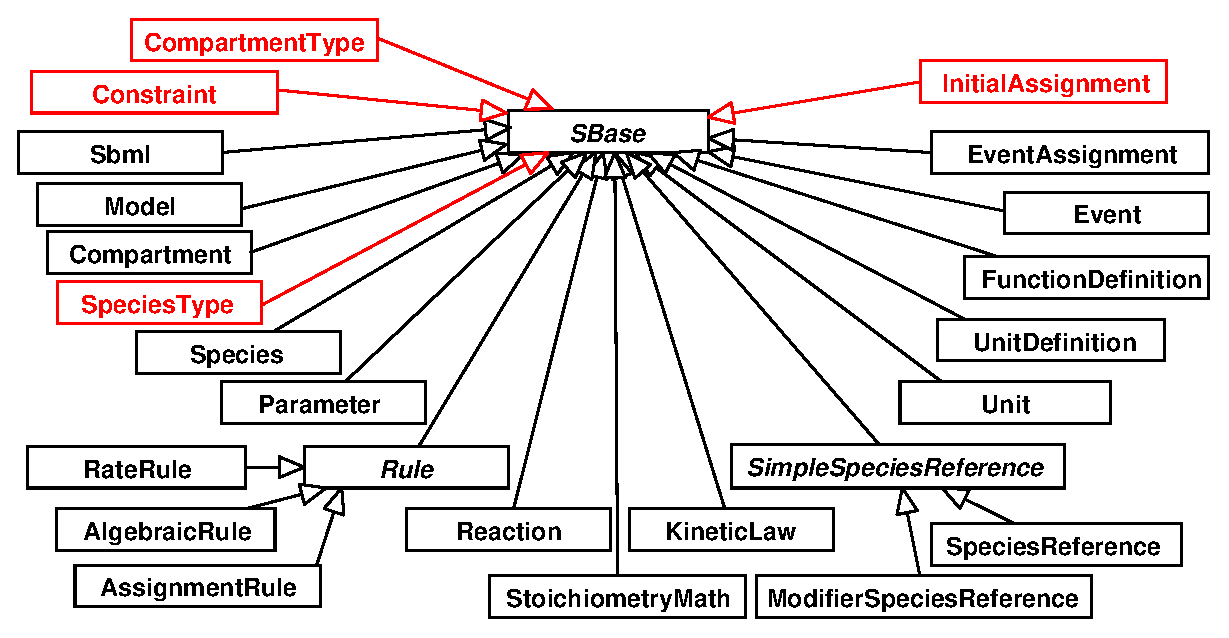
\includegraphics[scale = 0.7]{top-level}
  \caption{A UML diagram of the inheritance hierarchy of major data types
    in SBML.  Open arrows indicate inheritance, pointing from inheritors to
    their parents~\protect\citep{eriksson:1998,oestereich:1999}.  In addition to
    these types, all substructures in SBML (including, for example, all the
    \class{listOf} lists) are also derived from \class{SBase}.  See text
    for details.}
  \label{fig:top-level}
\end{figure}


%-----------------------------------------------------------------------------
\subsection{\changed{Type \class{SBase}}}
\label{sec:sbase}
%-----------------------------------------------------------------------------

Every structure composing an SBML Level~2 model definition has a specific
data type that is derived directly or indirectly from a single abstract
type called \class{SBase}.  This base type is designed to allow a modeler
or a software package to attach arbitrary information to each major
structure or list in an SBML model.  The definition of \class{SBase} is
presented in Figure~\vref{fig:sbase}.

In addition, the \class{listOf}\rule{0.5in}{0.5pt} lists and all
substructures such as \attrib{trigger} on \class{Event}
(Section~\ref{sec:events}) are also derived from \class{SBase}.  (However,
the \attrib{notes} and \attrib{annotation} elements contained inside
\class{SBase} and discussed below are not derived from \class{SBase}.)

\begin{figure}[hbt]
  \vspace*{8pt}
  \centering
  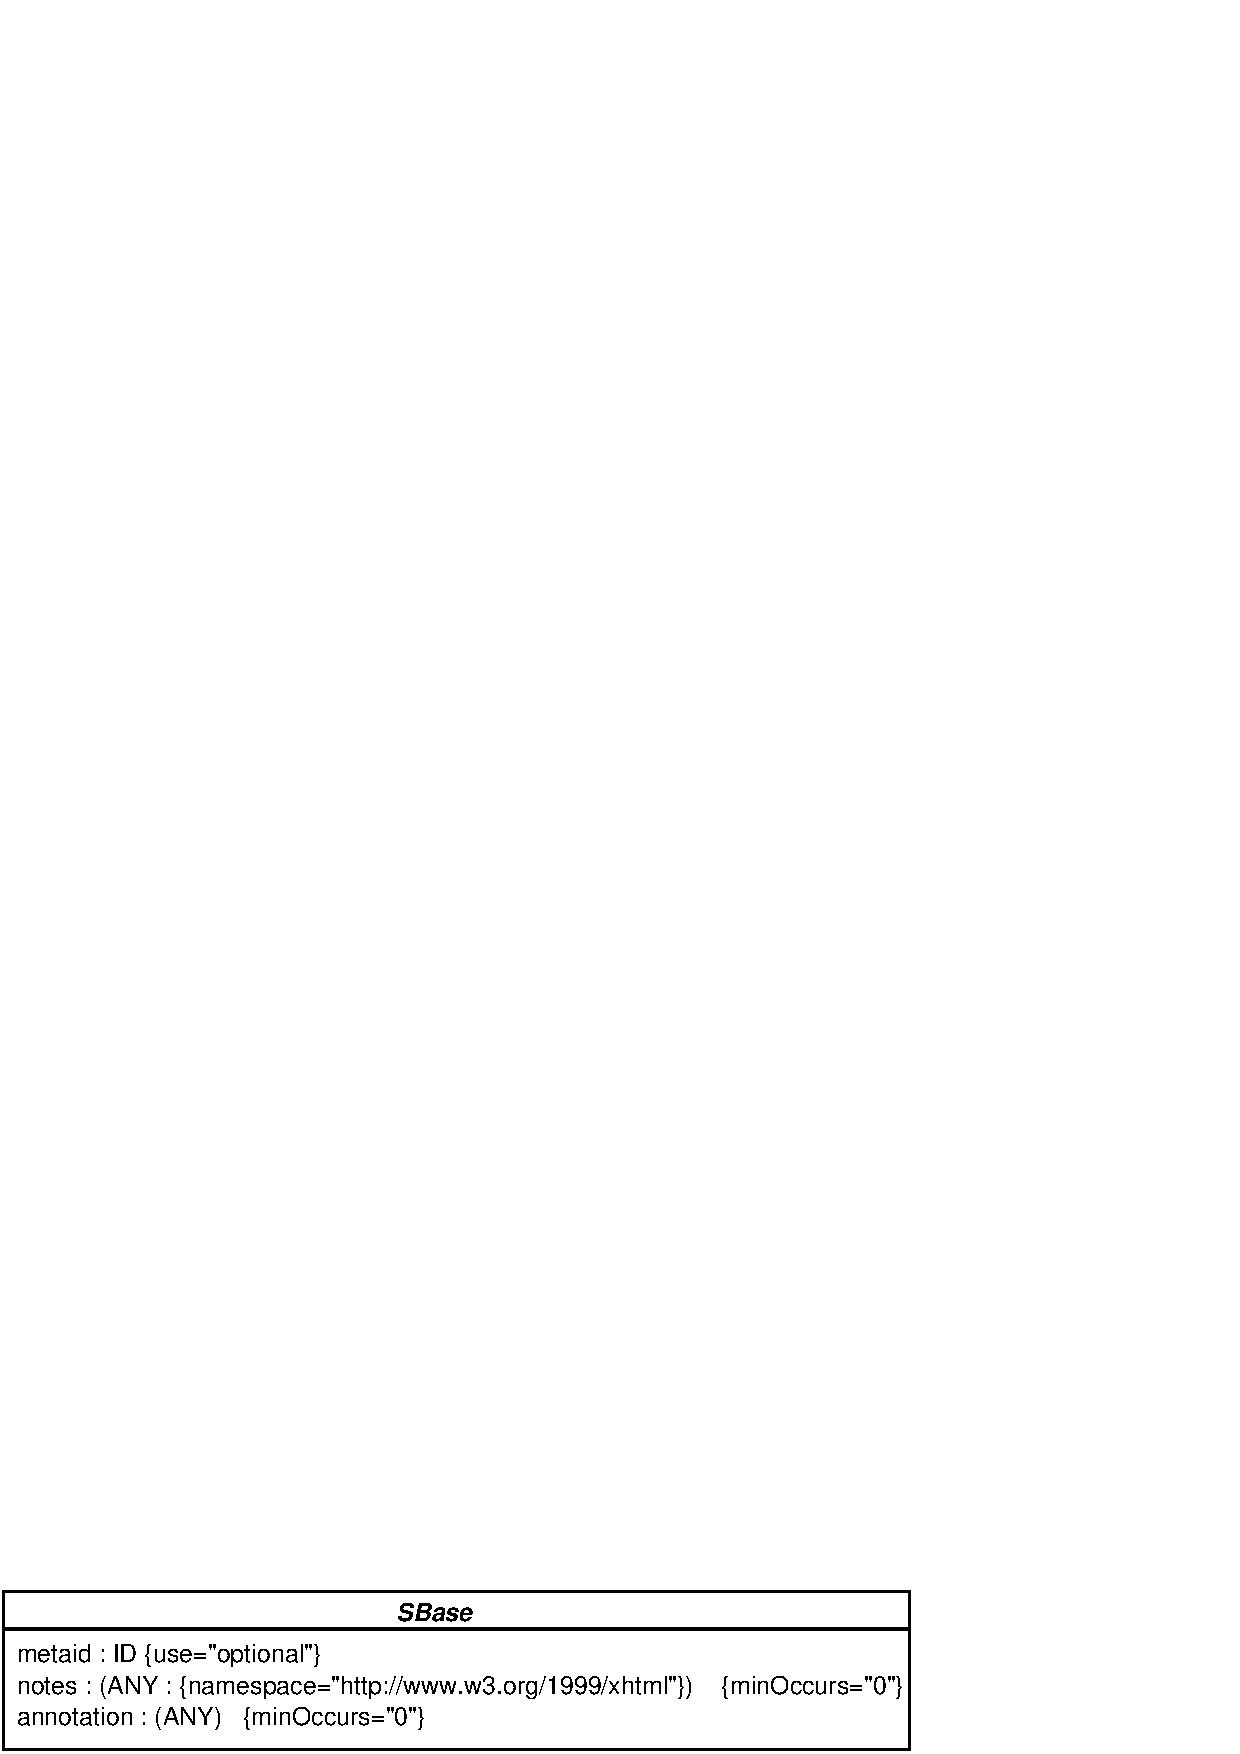
\includegraphics[scale = 0.7]{sbase}
  \caption{The definition of \class{SBase}.  Text enclosed in braces next
    to field types (e.g., \attribtype{\{minOccurs="0"\}}) indicates
    constraints on the possible field values.  We use the XML Schema
    language to express constraints because we are primarily interested in
    the XML encoding of SBML.  The constraint expression
    \attribtype{use="optional"} means that the indicated field is optional
    and may be omitted in a particular instance in a model.  The constraint
    expression \attribtype{minOccurs="0"} likewise means the indicated
    field is optional; this alternate form of expression must be used for
    those fields that are containers (i.e., fields encoded as
    subelements in XML).}
  \label{fig:sbase}
\end{figure}

\class{SBase} contains three fields, all of which are optional:
\attrib{metaid}, \attrib{notes} and \attrib{annotation}. These
fields are discussed separately in the following subsections.

\subsubsection{The \attrib{metaid} Field}

\begin{blockChanged}
The \attrib{metaid} field is present for supporting metadata
annotations using RDF~\cite[Resource Description
Format;][]{lassila:1999}.  It has a data type of XML \class{ID} (the
XML identifier type), which means each \attrib{metaid} value must be
globally unique within an SBML file.  The \attrib{metaid} value serves to
identify the element so that it can be referenced by metadata
placed within \class{annotation} structures (see Section~\ref{sec:annotation-use}).  Such
metadata can use RDF \class{description} elements in
which the RDF \attrib{describes} attributes contain the values of
the \attrib{metaid}'s of objects in the SBML model.
\end{blockChanged}

%The form of the RDF element content in SBML should follow the form
%described in the CellML Metadata
%Specification~\citep{cuellar:2002}.

\subsubsection{The \attrib{notes} Field}

The field \attrib{notes} in \class{SBase} is a container for XHTML content.
It is intended to serve as a place for storing optional information
intended to be seen by humans.  Typically, the \attrib{notes} field will contain
user comments about the structure in which the \attrib{notes} field is enclosed.
Every data object derived directly or
indirectly from type \class{SBase} can have a separate value for
\attrib{notes}, allowing users considerable freedom when adding comments to their
models.  Section~\ref{sec:examples} provides examples of using
\attrib{notes} in different models.


\begin{blockChanged}
\subsubsection{The \attrib{annotation} Field}
\label{sec:annotation-use}

Whereas the \attrib{notes} field described above is a container for content
to be shown directly to humans, the \attrib{annotation} field is a
container for optional software-generated content \emph{not} meant to be
shown to humans.  Every data object derived from \class{SBase} can have its
own value for \attrib{annotation}.  The field's data type is XML type
\class{any}, allowing essentially arbitrary data content.  SBML places only
a few restrictions on the organization of the content; these are intended
help software tools read and write the data as well as help reduce
conflicts between annotations added by different tools.

\paragraph{The Use of XML Namespaces in Annotations}

At the outset, software developers should keep in mind that multiple
software tools may attempt to read and write annotation content.  To reduce
the potential for collisions between annotations written by different
applications, \twotwo stipulates that tools must use XML
namespaces~\citep{bray:1999} to specify the intended vocabulary of every
annotation.  The application's developers must choose a URI
(\emph{Universal Resource Identifier}; \citealt{harold:2001,w3c:2000})
reference that uniquely identifies the vocabulary the application will use,
and a prefix string for the annotations.  Here is an example.  Suppose an
application uses the URI ``\texttt{http://www.mysim.org/ns}'' and the
prefix \texttt{mysim} when writing annotations related to screen layout.
The content of an annotation might look like the following:

\begin{example}
...
<annotation>
    <mysim:nodecolors xmlns:mysim="http://www.mysim.org/ns"
         mysim:bgcolor="green"
         mysim:fgcolor="white"/>
</annotation>
\end{example}

In this particularly simple case, the content consists of a single XML
element (\texttt{nodecolors}) with two attributes (\texttt{bgcolor},
\texttt{fgcolor}), all of which are prefixed by the string \texttt{mysim}.
(Presumably this particular content would have meaning to the hypothetical
application in question.)  The content in this particular example is small,
but it should be clear that it could easily have been an arbitrarily large
amount of data placed inside the \texttt{mysim:nodecolors} element.

The key point of the example above is that application-specific annotation
is entirely contained inside a single \emph{top-level element} within the
SBML \attrib{annotation} container.  \twotwo places the following
restrictions on annotations:

\begin{itemize}

\item Within a given SBML \attrib{annotation} element, there can only be
      one top-level element using a given namespace.

\item No top-level element in an \attrib{annotation} may use an SBML XML
      namespace, either explicitly by referencing an SBML XML namespace URI
      or implicitly by failing to specify any namespace on the annotation.
      (As of \twotwo, the defined SBML namespaces are the following URIs:
      ``\texttt{http://www.sbml.org/sbml/level1}'',
      ``\texttt{http://www.sbml.org/sbml/level2}'', as well as
      ``\texttt{http://www.sbml.org/sbml/level2/version2}''.)

\item The ordering of top-level elements within a given \attrib{annotation}
      element is \emph{not} significant.

\end{itemize}

The use of XML namespaces in this manner is intended to improve the ability
of multiple applications to place annotations on SBML model structures with
reduced risks of interference or name collisions.  Annotations stored by
different simulation packages can therefore coexist in the same model
definition.  The rules governing the content of \class{annotation} elements
are designed to enable applications to easily add, change, and remove their
annotations from SBML elements while simultaneously preserving annotations
inserted by other applications when mapping SBML from input to output.
    
Some more examples hopefully will make this more clear.  The next example
is invalid because it contains a top-level element in the SBML XML
namespace (because no namespace is declared, which means by default it
falls into the SBML namespace):

\begin{example}
<annotation>
    <cytoplasm/>
</annotation>
\end{example}

The following example is invalid because it contains two top-level elements
using the same XML namespace:

\begin{example}
<annotation>
    <mysim:nodecolors xmlns:mysim="http://www.mysim.org/ns"
        mysim:bgcolor="green" 
        mysim:fgcolor="white"/>
    <mysim:textcolors xmlns:mysim="http://www.mysim.org/ns"
        mysim:bgcolor="green" 
        mysim:fgcolor="white"/>
</annotation>
\end{example}

On the other hand, the following example is valid:

\begin{example}
<annotation>
    <mysim:geometry xmlns:mysim="http://www.mysim.org/ns" 
         mysim:bgcolor="green" mysim:fgcolor="white">
        <graph:node xmlns:graph="http://www.graph.org/ns" graph:x="4" graph:y="5" />
    </mysim:geometry>
    <othersim:icon xmlns:othersim="http://www.othersim.com/">
        WS2002
    </othersim:icon>
</annotation>
\end{example}

It is worth keeping in mind that although XML namespace names must be URI
references, an XML namespace name is \emph{not required} to be directly
usable in the sense of identifying an actual, retrieval document or
resource on the Internet~\citep{bray:1999}. The string
``\texttt{http://www.mysim.org/}'' is a namespace name or URI in the
examples above.  The approach is simply intended to enable unique
identification of constructs, and using URIs is a common and simple way of
creating a unique name string.

Finally, note that the namespaces being referred to here are XML namespaces
specifically in the context of the \attrib{annotation} field on
\class{SBase}.  The namespace issue here is unrelated to the namespaces
discussed in Section~\ref{sec:namespaces} in the context of \class{SId} and
symbols in SBML.


\paragraph{Content of Annotations and Implications for Software Tools}

The \attrib{annotation} field in the definition of \class{SBase}
exists in order that software developers may attach optional
application-specific data to the structures in an SBML model. However,
it is important that this facility not be misused.  In particular,
it is \emph{critical} that data essential to a model definition
\changed{or that can be encoded in existing SBML
structures} is \emph{not} stored in \attrib{annotation}. Parameter
values, functional dependencies between model structures, etc.,
should not be recorded as annotations.  It is crucial to keep in
mind the fact that data placed in annotations can be freely ignored by
software applications.  If such data changes the interpretation 
of a model, then software interoperability is greatly impeded.

Here are examples of the kinds of data that may be appropriately
stored in \attrib{annotation}: (a) information about the graphical
layout of model components; (b) application-specific processing
instructions that do not change the essential meaning of a model;
(c) identification information for cross-referencing
components in a model with items in a data resource.

\paragraph{Standardized Format for Certain Classes of Annotations}

For case (c) above (i.e., information for cross-referencing components in a
model to data resources), \twotwo recommends a standard format for use
within an \attrib{annotation} field.  This format should be used in
preference to proprietary syntaxes to maximize the likelihood that multiple
software tools will converge on the same syntax for this kind of
information.  The \twotwo recommended scheme is described in
Section~\ref{sec:finney-novere}.

\end{blockChanged}

%\begin{blockChanged}
%
%\subsubsection{The \attrib{definitionURL} Field}
%
%The field \attrib{definitionURL} in \class{SBase}, when present,
%must contain a Universal Resource Identifier (URI) string.  This URI
%associates the SBML object containing the field value with the
%resource referenced by the URI and indicates that the entity
%represented by the structure has a `is a' relationship with the
%resource.  A typical use of \attrib{definitionURL} is
%to reference an identifier in a controlled vocabulary.
%
%The field is named \attrib{definitionURL}, despite the fact that it would
%be better named ``definitionURI''.  The current name follows the name of
%the same field available on MathML~2.0 objects used in SBML.  Rather than
%introduce a ``definitionURI'' into SBML and thus require users and software
%to handle both names, SBML reluctantly follows the \attrib{definitionURL}
%name to reduce confusion and trivial typographical errors.
%
%Note that a URI is \emph{not} a URL and does not necessarily refer to a
%location on the World Wide Web.  Instead, a URI string is intended to be
%recognized by software applications as being an identifier for a resource
%which, in the simplest case, is purely conceptual.  For example, consider a
%set of software applications that share a common definition of the URI
%``\texttt{http://www.foobar.com/protein}'' as representing the concept of a
%protein.  The following fragment of SBML could indicate to those software
%applications that the species \texttt{MAPK} is a protein:
%
%\begin{example}
%<species id="MAPK" definitionURL="http://www.foobar.com/protein"/>
%\end{example}
%
%The presence of \attrib{definitionURL} on any SBML structure does not
%change the semantics of that structure as described in this document
%irrespective of any value contained in the field.  A parser wishing to
%interpret the mathematical or structural aspects of an SBML document can
%ignore \attrib{definitionURL} field values altogether.  (The use of
%\attrib{definitionURL} fields on MathML elements is covered by
%Section~\ref{sec:csymbol-token}.)
%
%Developers are advised and encouraged to take care when designing
%syntax schemes for URIs to ensure that schemes used by different
%application do not overlap.  One of the best ways of ensuring this is to use
%the Internet domain name of an appropriate organization as the
%base name for URIs.  (For example, this might be ``http://www.foobar.com''.)
%
%\end{blockChanged}



%%-----------------------------------------------------------------------------
%\subsection{Guidelines for the Use of the \attrib{definitionURL} Field in
%  \class{SBase}}
%\label{sec:definitionurl-use}
%%-----------------------------------------------------------------------------
%
%The presence of \attrib{definitionURL} on an SBML object \emph{must not
%  change the fundamental mathematical meaning} of the model.  An SBML model
%must stand on its own.  There are several reasons for this.  First, it
%would be too limiting to require that all software tools be able to load
%and parse the targets of the URIs.  One reason is that it is currently
%impossible to pick a standard format for the contents because there is no
%such agreed-upon standard format; moreover, as is the case in MathML~2.0,
%there will be times when a non-standard format is preferable, such as when
%a model author is exploring new ideas.  Second, allowing the use of
%\attrib{definitionURL} to alter the mathematical meaning of a model would
%reduce interoperability of SBML models.
%
%What \attrib{definitionURL} \emph{can} do is provide information that
%enriches a model in a way that can be used by suitably-designed software
%tools.  To take up the example of reaction rate equations, a
%\attrib{definitionURL} value on an SBML \class{Reaction} object could point
%to a controlled vocabulary term identifying the reaction as being a
%particular one in a conceptual hierarchy of reaction types.  This would be
%in addition to the mathematical formula supplied in the \texttt{kineticLaw}
%component of the reaction object.  Tools that were designed to interpret
%and recognize the controlled vocabulary terms could provide additional
%information to a human user (e.g., that a given reaction is in fact an
%instance of a non-competitive inhibitory reaction), but at the same time,
%tools that could not interpret the additional information would still be
%able to work with the mathematical formula as is the case in SBML today.


%-----------------------------------------------------------------------------
\subsection{The \attrib{id} and \attrib{name} Fields on SBML Components} 
\label{sec:idnameattribs}
%-----------------------------------------------------------------------------

As will become apparent below, most structures in SBML include two common
fields: \attrib{id} and \attrib{name}.  The \attrib{id} field is usually
required for most structures and is used to identify a component within the
model definition.  Other SBML structures can refer to the component using
this identifier.  Section~\ref{sec:id} provides a definition of the data type \class{SId}
used for the \attrib{id} field, and Section~\ref{sec:namespaces} describes
the scoping and namespace rules for these identifiers.  In
Section~\ref{sec:why-not-on-sbase}, we provide an explanation of why these
fields are not defined on \class{SBase}.

%-----------------------------------------------------------------------------
\subsubsection{Type \class{SId}}
\label{sec:id}
%-----------------------------------------------------------------------------

The type \class{SId} is the type of the \attrib{id} field found on the
majority of SBML components.  \class{SId} is a data type derived from the
basic XML type \class{string}, but with restrictions about the types of
characters permitted and the sequence in which they may appear.  Its
definition is shown in Figure~\vref{fig:id}.

\begin{figure}[htb]
  \vspace*{2pt}
  \ttfamily
  \centering
  \color{BrickRed}
  \begin{tabular}{lll}
    letter & ::= & 'a'..'z','A'..'Z'\\
    digit  & ::= & '0'..'9'\\
    idChar & ::= & letter | digit | '\_'\\
    SId    & ::= & ( letter | '\_' ) idChar*\\
  \end{tabular}
  \color{black}
  \caption{The definition of the type \class{SId} expressed in the variant
    of BNF used by the XML 1.0 specification~\protect\citep{bray:2000}.
    The characters \texttt{(} and \texttt{)} are used for grouping, and the
    character \texttt{*} indicates ``zero or more times''.}
  \label{fig:id}
\end{figure}

The equality of \class{SId} values is determined by an exact character sequence
match; i.e., comparisons of these identifiers must be performed in a
case-sensitive manner.  This applies to all uses of \class{SId} including
the identifiers of unit definitions.

The \class{SId} is purposefully not derived from the XML \class{ID} type.
Using XML's \class{ID} would force all SBML identifiers to exist in a
single global namespace, which would affect not only the form of local
parameter definitions but also future extensions for supporting
model/submodel composition.  Further, the use of the \class{ID} type for
SBML identifiers would have limited utility because MathML \class{ci}
elements are not of the type \class{IDREF} (see
Section~\ref{sec:formulas}).  Since the \class{IDREF}-\class{ID} linkage
cannot be exploited in MathML constructs, the utility of the XML \class{ID}
type is greatly reduced.


%-----------------------------------------------------------------------------
\subsubsection{Names}
\label{sec:names}
%-----------------------------------------------------------------------------

In contrast to the \attrib{id} field, the \attrib{name} field is optional
and is not intended to be used for cross-referencing purposes within a
model.  Its purpose instead is to provide a human-readable label for the
component.  The data type of the \attrib{name} field is the type
\class{string} defined in XML Schema~\citep{biron:2000,thompson:2000}.
This type includes all Unicode characters~\citep{unicode:1996} except for
two delimiter characters, 0xFFFE and 0xFFFF~\citep{biron:2000}.  In
addition, the following quoting rules specified by XML for character
data~\citep[][Section~2.4]{bray:2000} must be obeyed:
\begin{itemize}

\item The ampersand (\texttt{\&}) character must be escaped using the
  entity \texttt{\&amp;}.

\item \changed{The apostrophe (\texttt{'}) and  quotation mark
  (\texttt{"}) characters must be
  escaped using the entities \texttt{\&apos;} and \texttt{\&quot;}, respectively, when
  those characters are used to delimit a string attribute value.}

\end{itemize}
Other XML built-in character or entity references, e.g., \texttt{\&lt;} and
\texttt{\&x1A;}, are permitted.  SBML imposes no restrictions as to the
content of \attrib{name} fields beyond those restrictions defined by the
\class{string} type in XML Schema.

The recommended practice for handling \attrib{name} is as follows.  If a
software tool has the capability for displaying the content of
\attrib{name} fields, it should display this content to the user as a
component's label instead of the component's \attrib{id} field.  If the
user interface does not have this capability (e.g., because it cannot
display or use special characters in symbol names), or if the \attrib{name}
field is missing on a given component, then the user interface should
display the value of the \attrib{id} field instead.  (Script language
interpreters are especially likely to display \attrib{id} fields instead of
\attrib{name} fields.)

As a consequence of the above, authors of systems that automatically
generate the values of \attrib{id} fields should be aware some systems may
display the \attrib{id}'s to the user.  Authors therefore may wish to take
some care to have their software create \attrib{id} values that are
reasonably easy for humans to type and read.

\begin{blockChanged}
An additional point worth mentioning is although there are restrictions on
the uniqueness of \attrib{id} values (see Section~\ref{sec:namespaces}
below), there are no restrictions on the uniqueness of \attrib{name} values
in a model.  This allows software packages leeway in assigning
component identifiers.
\end{blockChanged}

%For example, a species in an SBML model must be
%located in a compartment, which means that if the same species appears in
%multiple compartments (e.g., in the context of a transport reaction), they
%must be given different identifiers.  It is currently the case that users
%and software differ sharply in philosophy about how to treat this
%situation: some treat these as different species, and others treat them as
%the same species located in different places.  Those in the latter group
%often want to use the same \attrib{name} but have different \attrib{id}
%values for the differently-localized ``instances'' of the species.  The
%freedom from restrictions on \attrib{name} values enables SBML to
%accommodate both philosophies.

%-----------------------------------------------------------------------------
\subsubsection{Component Identifiers and Namespaces in SBML}
\label{sec:namespaces}
%-----------------------------------------------------------------------------

A biochemical network model can contain a large number of
components representing different parts of a model.  This leads to
a problem in deciding the scope of an identifer: in what contexts
does a given identifier \emph{X} represent the same thing?  The
approaches used in existing simulation packages tend to fall into
two categories which we may call global and local.  The
\emph{global} approach places all identifiers into a single global
namespace, so that an identifier \emph{X} represents the same thing
wherever it appears in a given model definition.  The \emph{local}
approach places symbols in different namespaces depending on the
context, where the context may be, for example, individual reaction rate
expressions.  The latter approach means that a user may use the same
identifer \emph{X} in different rate expressions and have each instance
represent a different quantity.

The fact that different simulation programs may use different
rules for identifier resolution poses a problem for the exchange
of models between simulation tools.  Without careful
consideration, a model written out in SBML format by one program
may be misinterpreted by another program.  SBML Level~2 must
therefore include a specific set of rules for treating identifers
and namespaces.

The namespace rules in SBML Level 2 are relatively straightforward and are
intended to avoid this problem with a minimum of requirements on the
implementation of software tools:
\begin{itemize}

\item \changed{The identifiers (i.e., the values of the field
\attrib{id})
  of functions, compartments, species types, species, reactions,
  simple species references, events and model-level
  parameters reside in the same global namespace.  This means, for example,
  that a reaction and a species definition cannot both have the same
  identifier.}

\item Each reaction definition (see Section~\ref{sec:reactions})
  establishes a private local namespace for local parameter identifiers.
  Within the definition of a given reaction, local parameter identifiers
  introduced in that reaction override (shadow) identical identifers in the
  global namespace.

\item Unit identifiers (the values of the field \attrib{id} in the
  \class{UnitDefinition} structure) exist in a separate global namespace
  distinct from other identifiers.

\end{itemize}

The set of rules above can enable software packages using either local or
global namespaces for parameters to exchange SBML model definitions.  In
particular, software environments using local namespaces for parameters
internally should be able to accept SBML model definitions without needing
to change component identifiers.  Environments using a global namespace for
parameters internally can perform a simple manipulation of the identifiers
of local parameter elements within reaction definitions to avoid name
collisions.  (An example approach for the latter would be the following:
when receiving an SBML-encoded model, prefix each parameter identifier
inside each reaction with a string constructed from the reaction's
identifier; when writing an SBML-encoded model, strip off the prefix.)

The namespace rules described here will hopefully provide a clean
transition path to future levels of SBML, when submodels are introduced
(Section~\ref{sec:level-3}).  Submodels will provide the ability to compose
one model from a collection of other models.  This capability will have to
be built on top of SBML Level~2's namespace organization.  A
straightforward approach to handling namespaces is to make each submodel's
space be private.  The rules governing namespaces within a submodel can
simply be the Level~2 namespace rule described here, with each submodel
having its own (to itself, global) namespace.


%-----------------------------------------------------------------------------
\subsubsection{Identifiers, Names, and \class{SBase}}
\label{sec:why-not-on-sbase}
%-----------------------------------------------------------------------------

% [MH 2006-03-06] Most of the following issues could be addressed
% by having a separate "SBaseWithId" class.  I think only the first
% two reasons couldn't be addressed.  Thus, the original paragraph
% (which only talked about scoping) was almost in some sense the 
% fundamental reason.  I added this other stuff to address some
% questions made in the past, but these other arguments are all
% trumped by saying ``just define an SBaseWithID''.  Therefore, 
% it may be worth thinking about going back to the single reason.

\begin{blockChanged}
Although many SBML components also feature two other fields named
\attrib{id} and \attrib{name}, these fields are purposefully not defined on
\class{SBase}.  There are several reasons for this.

First, the identifier field is optional on some SBML components and
required on others.  Putting \attrib{id} on \class{SBase} would make it
impossible to accommodate both cases---it would force identifiers to be
mandatory on all components.  Second, the \class{SBase} abstract type is
used as the base type for certain structures such as \class{Unit},
\class{AssignmentRule}, \class{AlgebraicRule}, etc., which do not have
identifiers at all because they are subordinate to other structures that
\emph{do} have identifiers.  If instead \class{SBase} had an \attrib{id}
field, all objects of these other types in a model would then need to be
assigned unique identifiers.  This would be a needless burden on software
developers, given that these objects do not need identifiers.  Third, and
more importantly, the presence of an SBML identifier field (\attrib{id})
necessarily requires specifying scoping rules for the corresponding
identifiers.  However, the \class{SBase} abstract type is used as the basis
for defining components whose scoping rules are in some cases different
from each other.  (See Section~\ref{sec:namespaces} for more details).  If
\class{SBase} where to have an \attrib{id} field, then the specification of
\class{SBase} would need a default scoping rule and this would then have to
be overloaded on derived classes that needed different scoping.  This would
make the SBML specification needlessly complex.  Fourth, because
\class{SBase} is the base type of the \class{listOf}\rule{0.5in}{0.5pt}
lists (see Section~\ref{sec:type-inheritance-hierarchy}), putting
\attrib{id} on \class{SBase} would require all of these lists in a model to
be given identifers.  This would again be pointless because these lists are
only syntactic constructs; they cannot carry a value or be referenced by
the rest of an SBML model.  Finally, because the \class{Sbml} top-level
object is derived from \class{SBase}, it too would have to be assigned a
mandatory identifier.  Again, there is no functional reason to have an
identifier on this object (it is outside the model!).  With respect to the
\attrib{name} field, \class{SBase} does not have a \attrib{name} simply
because such a field is paired with an \class{id} field.
\end{blockChanged}



\begin{blockChanged}
%-----------------------------------------------------------------------------
\subsection{The \attrib{sboTerm} Field on SBML Components and the \class{SBOTerm} type}
\label{sec:sboTerm}
%-----------------------------------------------------------------------------

The structures \class{InitialAssignment},
\class{SimpleSpeciesReference}, \class{Parameter},
\class{KineticLaw}, \class{Rule}, \class{Model},
\class{Constraint} and \class{Reaction} all have \attrib{sboTerm}
optional fields of the type \class{SBOTerm}. These fields when
present must contain valid Systems Biology Ontology\sboref
identifiers that refer to actual SBO terms. The \class{SBOTerm}
type restricts the field values to strings of the form
\texttt{sbo:XXXXXXX} where \texttt{X} is a decimal digit. The
containing SBML structure should have an `is a' relationship with
the SBOTerm referenced by the \attrib{sboTerm} field.

SBO is a standard ontology that is not part of the SBML standard.
SBO will change independently of the SBML standard i.e. changes to
SBO will not be synchronized with new SBML levels and versions.
However the SBO development process will follow closely
conventional bioinformatics ontology development so that SBO term
identifiers will never be reassigned to new definitions.

Best practice for SBML generating software is to use the
\class{sboTerm} fields in preference to using application specific
annotation schemes.
\end{blockChanged}


%-----------------------------------------------------------------------------
\subsection{Mathematical Formulas in SBML Level 2}
\label{sec:formulas}
%-----------------------------------------------------------------------------

Mathematical expressions in SBML Level~2 are represented using
MathML~2.0~\citep{w3c:2000b}, the XML standard for describing
mathematics in machine-readable format.  It is used in the
definitions of functions (Section~\ref{sec:functions}), rules
(Section~\ref{sec:rules}), initial assignments
(Section~\ref{sec:initialAssignment}), constraints
(Section~\ref{sec:constraints}), reaction kinetics
(Section~\ref{subsec:kinetic-law}), stoichiometries
(Section~\ref{subsec:speciesreference}) and events
(Section~\ref{sec:events}). The \class{FunctionDefinition}, \class{KineticLaw},
\class{StoichiometryMath}, \class{EventAssignment},
\changed{\class{InitialAssignment}, \class{Constraint}}, and
\class{Rule} structures each have a single MathML \class{math}
subelement.  \changed{The \class{Event} structure has two \class{math} elements, one
inside a subelement named \attrib{trigger} and the other inside
a subelement named \attrib{delay}.  The \class{FunctionDefinition}'s single
\class{math} element is limited to containing only a single MathML
\class{lambda} element.}

The XML namespace URI for all MathML elements is
``\texttt{http://www.w3.org/1998/Math/MathML}''.  [See the W3C document by
\citet{bray:1999} for more information about using XML namespaces.]  The
examples \changed{throughout this specification} illustrate the use of this
namespace and MathML in SBML.

\changed{The semantic interpretation of MathML in the context of
SBML follows the MathML standard.  In particular, the
semantics of MathML functions follow the definitions
laid out by \cite{abramowitz:1997} and \cite{zwillinger:1988}.  
Readers are directed to these sources and the MathML specification
for information about such things as which principle values of the
inverse trigonometric functions to use.}

\subsubsection{Subset of MathML Used in SBML Level 2}
\label{sec:mathmlsubset}

The subset of MathML elements used in SBML Level~2 is similar to that used by
CellML~\changed{\citep{hedley:2001b}} and is itemized below:

\begin{itemize}\setlength{\parskip}{-0.2ex}

\item \emph{token}: \class{cn}, \class{ci}, \class{csymbol}, \class{sep}

\item \emph{basic content}: \class{apply}, \class{piecewise},
\class{piece}, \class{otherwise}

\item \emph{relational operators}:
            \class{eq}, \class{neq}, \class{gt}, \class{lt}, \class{geq}, \class{leq}

\item \emph{arithmetic operators}:
            \class{plus}, \class{minus}, \class{times},
            \class{divide}, \class{power}, \class{root},
            \class{abs}, \class{exp}, \class{ln}, \class{log},
            \class{floor}, \class{ceiling}, \class{factorial}

\item \emph{logical operators}:
            \class{and}, \class{or}, \class{xor}, \class{not}

\item \emph{qualifiers}:
            \class{degree}, \class{bvar}, \class{logbase}

\item \emph{trigonometric operators}:
            \class{sin}, \class{cos}, \class{tan}, \class{sec}, \class{csc}, \class{cot},
            \class{sinh}, \class{cosh}, \class{tanh}, \class{sech}, \class{csch}, \class{coth},
            \class{arcsin}, \class{arccos}, \class{arctan}, \class{arcsec}, \class{arccsc}, \class{arccot},
            \class{arcsinh}, \class{arccosh}, \class{arctanh}, \class{arcsech}, \class{arccsch}, \class{arccoth}

\item \emph{constants}:
            \class{true}, \class{false}, \class{notanumber},
            \class{pi}, \class{infinity}, \class{exponentiale}

\item \emph{annotation}:
            \class{semantics}, \class{annotation},
            \class{annotation-xml}
\end{itemize}

The inclusion of logical operators, relational operators,
\class{piecewise}, \class{piece}, and \class{otherwise} elements
facilitates the encoding of discontinuous expressions.  Elements for
representing partial differential calculus are not included.  We anticipate
that the requirements for partial differential calculus will be addressed
in proposals for SBML Level~3 geometry representations (see
Section~\ref{sec:level-3}).

\changed{Parsers should take particular note of the MathML
semantics of the N-ary operators \class{plus}, \class{times},
\class{and}, \class{or} and \class{xor}, when they are used
with different numbers of arguments.  The MathML
specification~\citep{w3c:2000b} appendix C.2.3 describes the
semantics for these operators with zero, one, and more arguments.}

The following are the only attributes permitted on MathML elements in SBML:

\begin{blockChanged}
\begin{itemize}\setlength{\parskip}{-0.2ex}
\item \attrib{style}, \attrib{class} and \attrib{id} on any
element;

\item \attrib{encoding} on \class{annotation},
\class{annotation-xml}, \class{csymbol} and \class{semantics} elements;

\item \attrib{definitionURL} on \class{annotation},
\class{annotation-xml}, \class{ci}, \class{csymbol} and \class{semantics} elements; and

\item \attrib{type} on \class{cn} elements.
\end{itemize}
\end{blockChanged}

Missing values for these attributes are to be treated in the same way as
defined by MathML.
These restrictions on attributes are designed to confine the MathML elements to their
default semantics and to avoid conflicts in the interpretation of the type of token
elements.

%\label{sec:mathmltokens}

\subsubsection{\changed{Handling of Whitespace}}
\label{sec:whitespace}

\begin{blockChanged}
MathML 2.0 defines ``whitespace'' in the same way as XML does, i.e., the
space character (Unicode hexadecimal code 0020), horizontal tab (code
0009), newline or line feed (code 000A), and carriage return (code 000D).
In MathML, the content of elements such as \class{cn} (described below) can
be surrounded by whitespace characters.  Prior to using the content, this
whitespace is ``trimmed'' from both ends: all whitespace at the beginning
and end of the content is removed~\cite{ausbrooks:2003}.

For example, in a MathML element \texttt{<cn> 42 </cn>}, the amount of
white space on either side of the ``\texttt{42}'' inside the \texttt{<cn>}
\ldots\ \texttt{</cn>} container does not matter.  Prior to interpreting
the content, the whitespace is removed altogether.
\end{blockChanged}


\subsubsection{Use of \class{cn} Elements in MathML Expressions in SBML}
\label{sec:cn-token}

\changed{The content of a \class{cn} element must be a number. The
number can be preceded and succeeded by whitespace.}

The following are the only permissible values for the
\attrib{type} attribute on MathML \class{cn} elements:
``\attribvalue{e-notation}'', ``\attribvalue{real}'',
``\attribvalue{integer}'', and ``\attribvalue{rational}''.  The
value of the \attrib{type} attribute defaults to
``\attribvalue{real}''.

\begin{blockChanged}
The values of the content of \class{cn} elements do not
necessarily conform to any specific floating point or integer
representations designed for CPU implementation. For example the
value of a \class{cn} element may exceed the maximum value that
can be stored in a IEEE 64 bit floating point number (IEEE 754).
This is different from the XML Schema type \class{double} that is
used in the definition floating point fields of structures in the
SBML namespace which \emph{is} restricted to IEEE double-precision
64-bit floating point type IEEE 754-1985.  (Integer fields in the
SBML namespace are only restricted by sign in some cases. The
absolute size of field integer values is not restricted.)

It is worth highlighting the fact that MathML uses a style of
scientific notation that differs from what is defined in XML Schema.
The MathML ``\attribvalue{e-notation}'' requires the mantissa and exponent to
be separated by one \texttt{<sep/>} element.  The mantissa must
be a real number and the exponent part must be a signed
integer.  This leads to expressions such as

\begin{example}
<cn type="e-notation"> 2 <sep/> -5 </cn>
\end{example}

for the number $2 \times 10^{-5}$.  It is especially
important to note that the expression

\begin{example}
<cn type="e-notation"> 2e-5 </cn>
\end{example}

is \emph{not valid} in MathML~2.0.  Elsewhere in SBML, when an
attribute value is declared to have type ``\attribtype{double}'' (a
type taken from XML Schema), the compact notation
``\texttt{2e-5}'' is in fact allowed, but not inside MathML.
This is a regrettable difference between two standards that SBML
replies upon, but it is not feasible to redefine these types
within SBML because the result would be incompatible with parser
libraries written to conform with the MathML and XML Schema
standards.  It is also not possible to use XML Schema to define
a data type for SBML attribute values permitting the use of the
\texttt{<sep/>} notation, because XML attribute values cannot contain
XML elements.
\end{blockChanged}


\subsubsection{Use of \class{ci} Elements in MathML Expressions in SBML}
\label{sec:ci-token}

\changed{The content of a \class{ci} element must be an SBML identifier
that is declared elsewhere in the model.  The identifier can be
preceded and succeeded by whitespace.} The set of possible
identifiers that can appear in a \class{ci} element depends on the
containing structure in which the \class{ci} is used:

\begin{itemize}

\item If a \class{ci} element appears in the body of a function definition
  \changed{(Section~\ref{sec:functions})}, the
  referenced identifier must be either (i) one of the declared arguments to
  that function, or (ii) the identifier of a previously defined function.

\item \changed{In all other situations, the referenced identifier must be the
  identifier of a species, compartment, parameter, function or reaction declared in
  the model.}  The following are the only possible interpretations of using
  such an identifier in SBML:

  \begin{itemize}

  \item \emph{Species identifier}: When a species identifier occurs in a
    \class{ci} element, it represents the quantity (\quantity{amount of substance}
    or \quantity{concentration}) of that species.
    The units associated with a species identifier are
    \emph{the units of the species}, defined in
    Section~\ref{sec:species-units}.

  \item \emph{Compartment identifier}: When a compartment identifier occurs
    in a \class{ci} element, it represents the size of the compartment.
    The units associated with the size of the compartment are those
    given on the \class{Compartment} structure that declares the identifier;
    see Section~\ref{sec:compartment-units}.

  \item \emph{Parameter identifier}: When a parameter identifier occurs in
    a \class{ci} element, it represents the \changed{numerical} value assigned to that
    parameter.  The units associated with the parameter value are the units
    assigned in its instance of a \class{Parameter} structure; see
    Section~\ref{sec:parameter-units}.

  \item \emph{Function identifier}: When a function identifier occurs in a
    \class{ci} element, it represents a call to that function.  Function
    references in MathML occur in the context of using MathML's
    \class{apply} and often involve supplying arguments to the function;
    see Section~\ref{sec:functions}.

  \item \changed{\emph{Reaction identifier}: When a reaction
    identifier occurs in a \class{ci} element, it represents the
    rate of the reaction, which is given by the kinetic law of the
    reaction if present.  The units associated with the reaction
    value are the units assigned to the \class{KineticLaw} structure
    contained within the \class{Reaction} structure; see
    Section~\ref{subsec:kinetic-law}.  (The units of the reaction
    identifier follow the defaults described in
    Section~\ref{subsec:kinetic-law} when the \class{KineticLaw}
    structure is not present.)}

  \end{itemize}

\end{itemize}

\changed{The content of \class{ci} elements outside a
\class{KineticLaw} and \class{FunctionDefinition} structures
always refer to objects declared in the top level global namespace;
i.e., SBML uses ``early binding'' semantics.  The only \class{ci}
elements that can represent parameters listed in a
\class{KineticLaw} structure are those \class{ci} elements
contained in the \class{KineticLaw} structure (see
Section~\ref{subsec:kinetic-law}).}


\subsubsection{Use of \class{csymbol} Elements in MathML Expressions in SBML}
\label{sec:csymbol-token}

SBML Level 2 uses the MathML \class{csymbol} element to denote certain
built-in mathematical entities without introducing reserved names into the
component identifier namespace.  The \attrib{encoding} field of
\class{csymbol} should be set to ``\attribvalue{text}''.  The
\attrib{definitionURL} should be set to one of the following predefined
SBML symbol URIs:
\begin{itemize}

\item \texttt{http://www.sbml.org/sbml/symbols/time}.  This represents the
  current simulation time.  The units of the current time entity are
  determined from the built-in \unit{time} of Table~\vref{tab:builtin}.

\item \texttt{http://www.sbml.org/sbml/symbols/delay}.  This represents a delay
  function.  The delay function has the form $delay(x, d)$, taking two
  \changed{MathML expressions as} arguments.  Its value is the value of argument
  $x$ at $d$ time units before the current time.  \changed{There are no
  restrictions on the form of $x$.} The units of the $d$ parameter
  are determined from the built-in \unit{time}.  \changed{The value of the $d$
  parameter, when evaluated, must be numerical and be greater than or equal to 0.}
  The \texttt{delay} function is useful
  for representing biological processes having a delayed response, but
  where the detail of the processes and delay mechanism is not relevant to
  the operation of a given model.

\end{itemize}

The following examples demonstrate these concepts.  The XML fragment below
encodes the formula $x + t$, where $t$ stands for time.
\begin{example}
<math xmlns="http://www.w3.org/1998/Math/MathML">
    <apply>
        <plus/>
        <ci> x </ci>
        <csymbol encoding="text" definitionURL="http://www.sbml.org/sbml/symbols/time">
            t
        </csymbol>
    </apply>
</math>
\end{example}

\begin{blockChanged}
In the fragment above, the use of the token \texttt{t} is mostly a
convenience for human readers---the string inside the \texttt{csymbol} could
have been almost anything, because it is essentially ignored by MathML
parsers and SBML.  Some MathML and SBML processors will take note of the
token and use it when presenting the mathematical formula to users, but the
token used has no impact on the interpretation of the model and it does not
enter into the SBML component identifier namespace.  In other words, the
content of the \class{csymbol} element is for rendering purposes only and
can be ignored by the parser.
\end{blockChanged}

As a further example, the following XML fragment encodes the equation
$k + delay(x, 0.1)$ or alternatively $k_t + x_{t - 0.1}$:
\begin{example}
<math xmlns="http://www.w3.org/1998/Math/MathML">
    <apply>
        <plus/>
        <ci> k </ci>
        <apply>
            <csymbol encoding="text" definitionURL="http://www.sbml.org/sbml/symbols/delay">
                delay
            </csymbol>
            <ci> x </ci>
            <cn> 0.1 </cn>
        </apply>
    </apply>
</math>
\end{example}

Note that the URI in the value of ``\attrib{definitionURL}'', as all
URIs, are intended to serve as unique identifiers and are not intended to
be dereferenced as Internet addresses.  

\begin{blockChanged}

\subsubsection{Math Expression Types}
\label{sec:mathmltype}

MathML operators in SBML each return results in one of two possible types:
boolean and numeric.  The following guidelines summarize the different
possible cases.

The relational operators (\class{eq}, \class{neq},
\class{gt}, \class{lt}, \class{geq}, \class{leq}), the logical
operators (\class{and}, \class{or}, \class{xor}, \class{not}), and
the boolean constants (\class{false}, \class{true}) always return
boolean values.  

The roots of the expression trees used in the following contexts must also
yield boolean values:

\begin{itemize}\setlength{\parskip}{-0.2ex}

\item the arguments of the MathML logical operators (\class{and},
\class{or}, \class{xor}, \class{not}); 

\item the second argument of a MathML \class{piece} operator;

\item the \attrib{trigger} field of an SBML \class{Event} structure; and

\item the \attrib{math} field of an SBML \class{Constraint} structure.

\end{itemize}

The roots of the expression trees used in the following contexts can
optionally yield boolean values:

\begin{itemize}\setlength{\parskip}{-0.2ex}

\item the arguments to the \class{eq} and \class{neq} operators;

\item the first arguments of MathML \class{piece} and \class{otherwise}
operators; and

\item the top level expression of a function definition.

\end{itemize}

The type of an operator referring to an SBML \class{FunctionDefinition} is
determined by the type of the top-level operator of the MathML expression
in the \attrib{math} field of the function definition.  This type may be
boolean or numeric.

All other operators, values and symbols return numeric results.

The type of expressions should be used consistently.  The set of
expressions that make up the first arguments of the \class{piece}
and \class{otherwise} operators within the same \class{piecewise}
operator should all return values of the same type. The arguments
of the \class{eq} and \class{neq} operators should return the same
type.

\end{blockChanged}

%\subsubsection{N-ary Operators}
%\label{sec:nary-operators}
%
%The use of N-ary operators (\class{add}, \class{times}, \class{and},
%\class{or} and \class{xor}) should follow their definition in the MathML
%specification.  However, the MathML specification does not define the
%semantics of the operators with zero or one operand.  Here we define the
%relevant semantics for SBML.  The general form of the operators is
%
%\begin{center}
%f($x_1$ ... $x_n$) = base\_operand operator $x_1$ operator \ldots\ $x_n$
%\end{center}
%
%where $n$ is any non-negative integer and base\_operand is a
%constant that is associated with the operator.  The base\_operand
%can be considered an additional hidden operand to the operator.
%Table~\ref{tab:baseoperands} gives the base operands for the N-ary
%operators of the MathML subset used in SBML.
%
%\begin{table}[bh]
%  \begin{blockChanged}
%  \small
%  \centering
%  \begin{tabular}{ll}
%    \toprule
%    Operator & Base Operand \\
%    \midrule
%    \class{add} & 0 \\
%    \class{times} & 1 \\
%    \class{and} & true \\
%    \class{or} & false \\
%    \class{xor} & false \\
%    \bottomrule
%  \end{tabular}
%  \vspace*{-0.95ex}
%  \caption{The base operands of the N-ary operators of the MathML subset in
%    SBML.}
%  \label{tab:baseoperands}
%  \end{blockChanged}
%\end{table}
%
%For example
%
%\begin{example}
%<apply>
%    <add/>
%<apply/>
%\end{example}
%
%returns $0 = 0$;
%
%\begin{example}
%<apply>
%    <add/>
%    <cn>7</cn>
%<apply/>
%\end{example}
%
%returns $7 = 0 + 7$; and
%
%\begin{example}
%<apply>
%    <add/>
%    <cn>7<cn/>
%    <cn>13<cn/>
%</apply>
%\end{example}
%
%returns $20 = 0 + 17 + 13$.
%
%Numerical computations involving the N-ary operators can be
%optimized by performing replacements on the operators when certain
%conditions apply.  Specifically, the operator can be replaced by
%the base\_operand if the operator has no operands; or by an
%operand if the operator has only one operand (i.e.,  the operator
%is equivalent to identity).
%\end{blockChanged}

%=============================================================================
\section{SBML Components}
\label{sec:elements}
%=============================================================================

In this section, we define each of the major data structures in SBML. To
provide illustrations of their use, we give partial model definitions in
XML.  Section~\ref{sec:xml-rep} provides many full examples of SBML in XML.

\begin{blockChanged}
In type definitions presented throughout this section section, we follow the UML
convention of hiding the attributes derived from a parent type such as
\class{SBase}. It should be kept in mind that these attributes are always
available.
\end{blockChanged}


%-----------------------------------------------------------------------------
\subsection{The SBML Container}
\label{sec:sbml}
%-----------------------------------------------------------------------------

The outermost portion of an SBML Level~2 model definition consists of a
single \class{Sbml} structure enclosing a single \class{Model} structure
(see next Section).  The definition of \class{Sbml} is shown in
Figure~\ref{fig:sbml}.

\begin{figure}[htb]
  \vspace*{6pt}
  \centering
  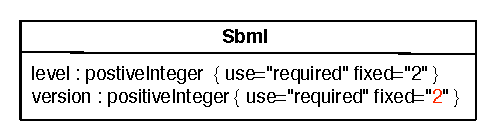
\includegraphics[scale = 0.9]{sbml}
  \caption{The definition of \class{Sbml} for SBML Level~2 \changed{Version~2}.  Following UML notation, additional fields
    that are inherited from a base class, in this case \class{SBase}, are not shown.}
  \label{fig:sbml}
\end{figure}

\changed{The XML namespace URI for SBML Level~2 Version~2 is
``\texttt{http://www.sbml.org/sbml/level2/version2}''}.  All SBML
Level~2 Version~2 elements should be encoded using this URI by
assigning \changed{it} to either the default \changed{XML} namespace or a tag
prefix.  The character encoding for SBML is UTF-8.  SBML documents
should include the \attrib{encoding} attribute with the value
\attribvalue{UTF-8} in the XML prologue.

In the transformation of UML to XML used in this document, the \class{Sbml}
structure is turned into an element named \texttt{sbml}.  The element has
two required attributes: \attrib{level} and \attrib{version}.  \changed{For SBML
Level~2 Version~2, these attributes must be set to ``\texttt{2}'' and
``\texttt{2}'', respectively.}

The following is an abbreviated example of the outermost content of an SBML
model definition in XML:

\begin{blockChanged}
\begin{example}
<?xml version="1.0" encoding="UTF-8"?> 
<sbml xmlns="http://www.sbml.org/sbml/level2/version2" level="2" version="2">
  ...
</sbml>
\end{example}
\end{blockChanged}

\begin{blockChanged}
Readers may wonder why the SBML top-level XML element uses both a namespace
URI identifying the SBML level and version, as well as separate XML
attributes encoding the level and version.  Why is the information
duplicated in this way?  There are several reasons.  First, XML is only one
possible serialization of SBML (albeit an extremely popular one at this
time).  Though most of this document is written with XML in mind, it is the
intention behind the design of SBML that its object structure should be
implementable in other languages and software systems.  For this reason,
the level and version information must be made available as explicit data
fields somewhere in a model.  Second, tools that use generic high-level XML
parsers may not be given access to the value of the \texttt{xmlns}
attribute.  Providing the information via separate attributes is a good
backup measure.  Third, earlier in the history of SBML, it was expected
that only the level needed to be encoded as part of the namespace URI
(e.g., ``\texttt{http://www.sbml.org/sbml/level1}'') because it was hoped
that changes within levels would not require XML Schema changes.  This has
proven to be false, but both versions of SBML Level~1 and the first version
of SBML Level~2 still subscribe to this principle.  This means that for
these variants of SBML, software tools must look for a \attrib{version}
attribute on the top-level element.  For backwards compatibility with
software that expects this, it makes more sense to keep the version and
level attributes.  And finally, XML namespaces have certain rules that
stymie straightforward pattern-matching recognition in such things as XSLT
transformations.  The full details would be beyond the scope of this
section, but the consequences are that it is simpler and more reliable to
match and extract information from attributes than from XML namespaces.
\end{blockChanged}


%One of them is that if an attribute name is not explicitly declared to be
%in a particular XML namespace, then that name is (paradoxically) not in
%\emph{any} XML namespace.  However, when it comes to namespaces in XML, all
%of the following are legal:
%\begin{example}
%<sbml xmlns="http://www.sbml.org/sbml/level2/version2" level="2" version="2">
%<sbml:sbml xmlns:sbml="http://www.sbml.org/sbml/level2/version2" level="2" version="2">
%<foo:sbml xmlns:foo="http://www.sbml.org/sbml/level2/version2" level="2" version="2">
%\end{example}
%XML parsers would return ``\texttt{xmlns}'', ``\texttt{xmlns:sbml}'', and
%``\texttt{xmlns:foo}'', respectively, for the namespace attribute.  The
%consequence is this: a pattern-matching system such as XSLT could match the
%\texttt{level} and \texttt{version} attributes regardless of which of these
%alternatives was presented (because of the paradoxical nature of
%unqualified attributes in namespaces), but properly detecting the namespace
%setting requires more complicated parsing to allow for any variation in
%namespace prefixes.  (After all, there may be other namespace declarations
%on the top-level \texttt{sbml} element, so simply looking for
%\texttt{xmlns} is not enough, nor is it enough to detect the SBML namespace
%URI string, since the string might be present but its use combined with the
%prefix might still be incorrect.) 


%-----------------------------------------------------------------------------
\subsection{Models}
\label{sec:model}
%-----------------------------------------------------------------------------

The \class{Model} structure is the highest-level construct in an SBML data
stream or document.  Its definition is shown in
Figure~\vref{fig:model}.  Only one component of type \class{Model} is
allowed per instance of an SBML document or data stream, although it does
not necessarily need to represent a single biological entity.

\begin{figure}[htb]
  \centering
  
\includegraphics[scale = 0.68]{model}
  \caption{The definition of \class{Model}.  Following UML notation, additional fields
    that are inherited from a base class, in this case \class{SBase}, are not shown.}
  \label{fig:model}
\end{figure}

\changed{\class{Model} serves as a container for
\class{FunctionDefinition}, \class{UnitDefinition},
\class{CompartmentType}, \class{Compartment}, \class{SpeciesType},
\class{Species}, 
\class{Parameter}, \class{InitialAssignment},
\class{Rule}, \class{Constraint}, \class{Reaction} and
\class{Event} components.} All of these components are optional;
that is, the lists in each of the respective fields are permitted
to have zero length. (However, there are dependencies between
components, such that defining some requires defining others.  For
example, as explained in other sections below, defining a species
requires defining a compartment, and defining a reaction requires
defining a species.)

The \class{Model} structure has an optional field, \attrib{id}, used to
give the model an identifier.  The identifier must be a text string
conforming to the syntax permitted by the \class{SId} data type described
in Section~\ref{sec:id}.  \class{Model} also has an optional \attrib{name}
field, of type \class{string}.  The \attrib{name} and \attrib{id} fields
\changed{must} be used as described in Section~\ref{sec:idnameattribs}.

\changed{In the XML encoding of an SBML model, the lists of
compartment types, compartments, species types, species, unit definitions,
parameters, initial assignments, reactions, function definitions, rules and events are
translated into lists of XML elements enclosed within elements of
the form \class{listOf}\rule{0.5in}{0.5pt}\class{s}, where the
blank is replaced by the name of the component type (e.g.,
``\texttt{Reaction}'').} The resulting XML data object has the
form illustrated by the following skeletal model:

\begin{blockChanged}
\begin{example}
<model id="My_Model">
    <listOfFunctionDefinitions>
        ...
    </listOfFunctionDefintions>
    <listOfUnitDefinitions>
        ...
    </listOfUnitDefinitions>
    <listOfCompartmentTypes>
        ...
    </listOfCompartmentTypes>
    <listOfCompartments>
        ...
    </listOfCompartments>
    <listOfSpeciesTypes>
        ...
    </listOfSpeciesTypes>
    <listOfSpecies>
        ...
    </listOfSpecies>
    <listOfParameters>
        ...
    </listOfParameters>
    <listOfInitialAssignments>
        ...
    </listOfInitialAssignments>
    <listOfRules>
        ...
    </listOfRules>
    <listOfConstraints>
        ...
    </listOfConstraints>
    <listOfReactions>
        ...
    </listOfReactions>
    <listOfEvents>
        ...
    </listOfEvents>
</model>
\end{example}
\end{blockChanged}

Readers may wonder about the motivations for the
\class{listOf}\rule{0.5in}{0.5pt}\class{s} notation.  A simpler
approach to creating the lists of components would be to place
them all directly at the top level under \texttt{<model> ...
</model>}.  We chose instead to group them within XML elements
named after \class{listOf}\rule{0.5in}{0.5pt}\class{s}, because we
believe this helps organize the components and makes visual
reading of model definitions easier.  These
\class{listOf}\rule{0.5in}{0.5pt}\class{s} elements are derived
from \class{SBase} which enables each list to contain its own
\attrib{metaid}, \attrib{notes} and \attrib{annotation}
 fields. Further details of how
\class{listOf}\rule{0.5in}{0.5pt}\class{s} elements implement UML
lists is described in Section~\ref{sec:notation}.


\begin{blockChanged}
\subsubsection{The \attrib{sboTerm} Field}

The \class{Model} structure has an optional \class{SBOTerm} field,
\attrib{sboTerm} (see Section~\ref{sec:sboTerm}).  This field when
present must contain an Systems Biology Ontology (SBO)\sboref term
identifier referring to a modeling framework SBO term, that is a
term derived from \sbomodellingframework. The SBO term chosen
should be the most precise (narrow) term that defines the
mathematical framework used in the model.
\end{blockChanged}

%-----------------------------------------------------------------------------
\subsection{Function Definitions}
\label{sec:functions}
%-----------------------------------------------------------------------------

The \class{FunctionDefinition} structure associates an identifier with a
function definition.  This identifier can then be used in any subsequent
MathML \class{apply} elements.  \class{FunctionDefinition} is shown in
Figure~\ref{fig:mathdefinition}.

\begin{figure}[htb]
  \vspace*{8pt}
  \centering
  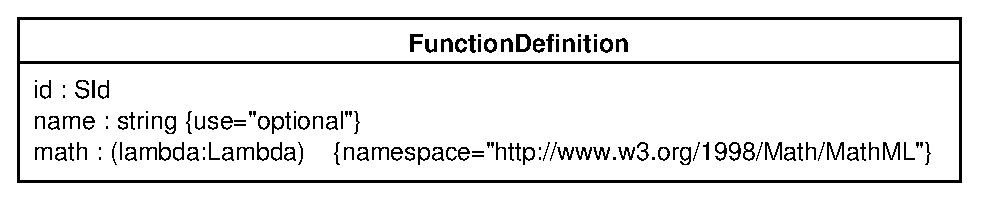
\includegraphics[scale = 0.68]{mathdefinition}
  \caption{The definition of \class{FunctionDefinition}.  Following UML notation,
    additional fields
    that are inherited from a base class, in this case \class{SBase}, are not shown.}
  \label{fig:mathdefinition}
\end{figure}

The \class{FunctionDefinition} structure has three fields: \attrib{id},
\attrib{name} and \attrib{math}.  Their purposes are explained in the
following subsections.

\subsubsection{The \attrib{id} and \attrib{name} Fields}

The \attrib{id} and \attrib{name} fields have types \class{SId}
and \class{string}, respectively, and operate in the manner
described in Section~\ref{sec:idnameattribs}.  \changed{MathML
\texttt{ci} elements in an SBML model can refer to the function defined by a
\class{FunctionDefinition} using the value of its \attrib{id}
field.}

\subsubsection{The \attrib{math} Field}
\label{sec:function-definition-math}

The \attrib{math} field is a container for MathML content that
defines the function.  The content of this field can only be a
MathML \texttt{lambda} element.  This is the only place in SBML
where a \texttt{lambda} element can be used. The function is only
available for use in other MathML elements that follow the
\class{FunctionDefinition} structure in an SBML model.  (These
restrictions prevent recursive and mutually-recursive functions
from being expressed.)  \changed{The \texttt{lambda} element
must begin with zero or more \texttt{bvar} elements, followed
by any other of the elements in the MathML subset listed in
Section~\ref{sec:mathmlsubset} \emph{except} \texttt{lambda}.
(I.e., a \texttt{lambda} element cannot contain another
\texttt{lambda} element.)}

The following abbreviated SBML example shows a \class{FunctionDefinition}
structure defining $pow3(x)$ as representing $x^{3}$:
\begin{example}
<model>
    ...
    <functionDefinition id="pow3">
        <math xmlns="http://www.w3.org/1998/Math/MathML">
            <lambda>
                <bvar><ci> x </ci></bvar>
                <apply>
                    <power/>
                    <ci> x </ci>
                    <cn> 3 </cn>
                </apply>
            </lambda>
        </math>
    </functionDefinition>
    ...
</model>
\end{example}


%-----------------------------------------------------------------------------
\subsection{Unit Definitions}
\label{sec:unitdefinitions}
%-----------------------------------------------------------------------------

Units may be supplied in a number of contexts in an SBML model. The units
of the following mathematical entities can be specified explicitly: constants,
initial conditions, symbols in formulas and the results of formulas.
Rather than having to give a complete unit definition
on every structure, SBML provides a facility
for defining identified units which can be reused throughout a model.
In addition, by default, SBML mathematical entities have units composed from
built-in units in a consistent fashion (see Sections~\ref{sec:built-in-units},
\ref{sec:compartment-units}, \ref{sec:species-units} and~\ref{subsec:kinetic-law}).
By redefining the built-in units it is possible to change the units
used throughout a model in a simple and consistent manner.

The SBML \class{UnitDefinition}  and
\class{Unit} structures enable combinations of units to
be given abbreviated names, and enable built-in units to be redefined.
The definitions of \class{UnitDefinition}  and
\class{Unit} are shown in
Figure~\vref{fig:unitdefinition}.

\begin{figure}[htb]
  \centering
  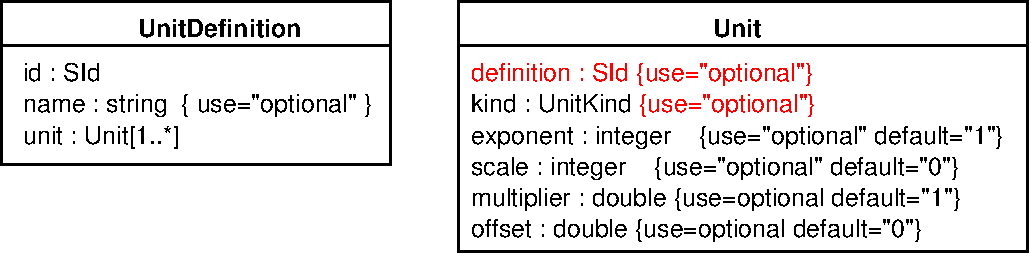
\includegraphics[scale = 0.68]{unitdefinition}
  \caption{The definition of \class{UnitDefinition} and \class{Unit}. Following UML
    notation, additional fields
    that are inherited from a base class, in this case \class{SBase}, are not shown.}
  \label{fig:unitdefinition}
\end{figure}


\subsubsection{The \class{UnitDefinition} Structure}
\label{sec:unitdefinition-structure}

An instance of a \class{UnitDefinition} consists of an \attrib{id}
field of type \class{SId}, an optional string field \attrib{name}
and a list of structures of type \class{Unit}.  As mentioned in
Section~\ref{sec:namespaces}, unit identifiers defined by the
\attrib{id} field are considered to be in a separate global
namespace distinct from the namespace of other identifiers in a
model; thus, unit identifiers cannot collide with the identifiers
of species, compartments, reactions, etc. \changed{The \attrib{id}
field must not contain a value from Table~\ref{tab:unitkind}, the
table of \class{UnitKind} values, ensuring that the units listed
in that table can always be referenced throughout a model.}

The approach to defining units in SBML is compositional; for example,
$meter\ second^{\,-2}$ is constructed by combining, within the same
\class{UnitDefinition} \class{Unit} list, a \class{Unit} structure representing
$meter$ with a \class{Unit} structure representing $second^{\,-2}$.
The \class{Unit} structure is described in the next subsection.


\subsubsection{The \class{Unit} Structure}
\label{sec:unit-structure}

The \class{Unit} data structure has one required field,
\attrib{kind}, whose value must be taken from \class{UnitKind}, an
enumeration of base units.  The possible values of
\class{UnitKind} are given in Table~\vref{tab:unitkind}.

%\changed{A \class{Unit} data structure is a component of a
%\class{UnitDefinition}.  A \class{Unit} structure defines a
%variant of another unit or simply a reference to another unit. The
%other unit must be defined elsewhere either in the enclosing
%\class{Model} with a \class{UnitDefinition} structure or in the
%SBML specification. To define a variant of, or simply reference,
%a unit defined in the SBML specification, the \class{Unit} structure has a
%optional field, \attrib{kind}, whose value must be taken from
%\class{UnitKind}, an enumeration of base units. The possible
%values of \class{UnitKind} are given in Table~\vref{tab:unitkind}.
%To define a variant of, or simply reference, a unit defined with a
%\class{UnitDefinition} structure, \class{Unit} has an optional
%\class{SId} field, \attrib{definition}, which must refer to a
%\class{UnitDefinition} structure.}

\begin{table}[bht]
  \centering
  \ttfamily
  \begin{tabular}{llllll}
    \toprule
    ampere      & farad & joule     & lux       & radian   & volt   \\
    becquerel   & gram  & katal     & metre     & second   & watt\\
    candela     & gray  & kelvin    & mole      & siemens  & weber\\
    Celsius     & henry & kilogram  & newton    & sievert\\
    coulomb     & hertz & litre     & ohm       & steradian\\
    \underline{dimensionless} & \underline{item} & lumen     & pascal    & tesla\\
    \bottomrule
  \end{tabular}
  \caption{The possible values of \attrib{kind} in a \class{UnitKind}
    structure.  All are names of base or derived SI
    units~\protect\citep{bipm:2000}, except for
    ``\texttt{dimensionless}'' and ``\texttt{item}'', which are
    SBML additions important for handling certain common situations.
    ``\texttt{Dimensionless}'' is intended for cases where a quantity does not
    have units, and ``\texttt{item}'' for expressing
    such things as ``N items'' (e.g., ``100 molecules'').
    Also, note that the gram and litre are not
    strictly part of SI; however, they are so
    commonly used in SBML's areas of application that they
    are included as predefined unit names.  (The standard SI unit of
    mass is in fact the kilogram, and volume is
    defined in terms of cubic meters.)}
  \label{tab:unitkind}
\end{table}

%\changed{A \class{Unit} structure must have one and only one
%\attrib{kind} or \attrib{definition} field value.  A \class{Unit}
%structure must not create a \class{UnitDefinition} structure where
%the \class{UnitDefinition} refers to itself directly or
%indirectly. (More specifically, consider the directed graph formed with vertices
%representing \class{UnitDefinition} structures and edges
%representing \attrib{definition} attribute values on \class{Unit}
%structures. The source of each edge is a vertex representing a
%\class{UnitDefintion} structure.  The sink of each edge is the
%vertex representing a \class{UnitDefinition} referenced by a
%\attrib{definition} attribute enclosed by the source
%\class{UnitDefinition} structure. Such directed graphs must be
%acyclic.)}

%\changed{The formula for a single transformation represented by a
%\class{Unit} structure is as follows (where $u$ is the original
%unit and $u_\emph{new}$ is the new unit):
%\begin{equation}
%\label{eq:single-unit-transformation}
%  u_\emph{new} = (\emph{multiplier} \times 10^\emph{scale}
%  \times u)^\emph{exponent} + \emph{offset}
%\end{equation}}
%The optional \attrib{exponent} field on \class{Unit} represents an exponent
%on the unit.  Its default value is ``\attribvalue{1}'' (one).  For the
%example mentioned at the beginning of this section, $second^{\,-2}$ would
%be obtained by using \texttt{kind="second"} and \texttt{exponent="-2"}.  A
%\class{Unit} structure also has an optional \attrib{scale} field; its value
%must be an integer exponent for a power of ten multiplier used to set the
%scale of the unit.  For example, a unit having a \attrib{kind} value of
%``\attribvalue{gram}'' and a \attrib{scale} value of ``\attribvalue{-3}''
%signifies $10^{-3} * gram$, or milligrams.  The default value of
%\texttt{scale} is ``\attribvalue{0}'' (zero), because $10^0 = 1$.
%
%\changed{The optional \attrib{multiplier} field can be used to
%multiply the original unit by a real-numbered factor; this enables
%the definition of units that are not power-of-ten multiples of SI
%units.}  For instance, a \attrib{multiplier} of 0.3048 could be
%used to define ``foot'' as a measure of length in terms of a
%metre.  The \attrib{multiplier} field has a default value of
%``\attribvalue{1}'' (one).  Finally, the \attrib{offset} field is
%used to represent the addition of a constant in the transformation
%of the \attrib{kind} unit.  For example, an \attrib{offset} value
%of ``\attribvalue{32.0}'' would be needed to define Fahrenheit in
%terms of degrees Celsius.  The \attrib{offset} field has a default
%value of ``\attribvalue{0}'' (zero).

Note that the set of acceptable values for the field \attrib{kind}
does not include units defined by \class{UnitDefinition}
structures.  This means that the units definition feature in SBML
is not hierarchial---user-defined units cannot be built on top of
other user-defined units, only on top of base units.  (SBML
differs from CellML in this respect; CellML allows the
construction of hierarchial unit definitions.)

A \class{Unit} structure represents a (possibly transformed)
reference to a base unit chosen from \class{UnitKind}.  The
formula for a single transformation represented by a \class{Unit}
structure is as follows (where $u$ is the original base unit and
$u_\emph{new}$ is the new unit):
\begin{equation*}
  u_\emph{new} = (\emph{multiplier} \times 10^\emph{scale}
  \times u^\emph{exponent}) + \emph{offset}
\end{equation*}
The optional \attrib{exponent} field on \class{Unit} represents an
exponent on the unit.  Its default value is ``\attribvalue{1}''
(one).  For the example mentioned at the beginning of this
section, $second^{\,-2}$ would be obtained by using
\texttt{kind="second"} and \texttt{exponent="-2"}.  A \class{Unit}
structure also has an optional \attrib{scale} field; its value
must be an integer exponent for a power of ten multiplier used to
set the scale of the unit.  For example, a unit having a
\attrib{kind} value of ``\attribvalue{gram}'' and a \attrib{scale}
value of ``\attribvalue{-3}'' signifies $10^{-3} * gram$, or
milligrams.  The default value of \texttt{scale} is
``\attribvalue{0}'' (zero), because $10^0 = 1$.

The optional \attrib{multiplier} field can be used to multiply the
\attrib{kind} unit by a real-numbered factor; this enables the
definition of units that are not power-of-ten multiples of SI
units.  For instance, a \attrib{multiplier} of 0.3048 could be
used to define ``foot'' as a measure of length in terms of a
metre.  The \attrib{multiplier} field has a default value of
``\attribvalue{1}'' (one).  Finally, the \attrib{offset} field is
used to represent the addition of a constant in the transformation
of the \attrib{kind} unit.  For example, an \attrib{offset} value
of ``\attribvalue{32.0}'' would be needed to define Fahrenheit in
terms of degrees Celsius.  The \attrib{offset} field has a default
value of ``\attribvalue{0}'' (zero).

The composition of $n$ \class{Unit} structures within a
\class{UnitDefinition} to create more complex units involves a
linear product according to the following formula:

\begin{blockChanged}
\begin{equation} \label{eq:multiple-unit-transformation}
  u_\emph{new} = m_1 \times \ldots \times m_n
  \times 10^{s_1} \times \ldots \times 10^{s_n}
  \times u^{e_1} \times \ldots \times u^{e_n}
\end{equation}
\end{blockChanged}

%\begin{blockChanged}
%Formula~\ref{eq:single-unit-transformation}, representing
%a \class{Unit} structure, $u$ refers to either a member of the
%\class{UnitKind} enumeration through the \attrib{kind} field or to
%a \class{UnitDefinition} through the \attrib{definition} field.
%In the latter case both
%Formulas~\ref{eq:single-unit-transformation}
%and~\ref{eq:multiple-unit-transformation} are applied recursively
%to each \class{UnitDefinition} until a \class{UnitKind} unit is
%reached.
%\end{blockChanged}

The following example illustrates the definition of an abbreviation named
``\unit{mmls}'' for the units $mmol\ l^{-1}\ s^{-1}$:

\begin{example}
<listOfUnitDefinitions>
    <unitDefinition id="mmls">
        <listOfUnits>
            <unit kind="mole"   scale="-3"/>
            <unit kind="litre"  exponent="-1"/>
            <unit kind="second" exponent="-1"/>
        </listOfUnits>
    </unitDefinition>
</listOfUnitDefinitions>
\end{example}

The following example defines Fahrenheit:

\begin{example}
<unitDefinition id="Fahrenheit">
     <listOfUnits>
         <unit kind="Celsius" multiplier="1.8" offset="32"/>
     </listOfUnits>
</unitDefinition>
\end{example}

%\begin{blockChanged}
%The following example defines minutes in terms of seconds and then
%hours in terms of minutes.
%
%\begin{example}
%<unitDefinition id="Minute">
%     <listOfUnits>
%         <unit kind="second" multiplier="60"/>
%     </listOfUnits>
%</unitDefinition>
%<unitDefinition id="Hour">
%     <listOfUnits>
%         <unit definition="Minute" multiplier="60"/>
%     </listOfUnits>
%</unitDefinition>
%\end{example}
%\end{blockChanged}

\subsubsection{Built-in Units}
\label{sec:built-in-units}

There are five special unit names in SBML, listed in
Table~\vref{tab:builtin}, corresponding to the five types of quantities or
\emph{built-in units} that play roles in biochemical reactions: amount of
substance, volume, area, length and time.
All SBML mathematical entities apart from parameters have default units.
These default units are composed from the set of \emph{built-in units}.
Further SBML defines defaults for the
built-in units, listed in the third column of Table~\ref{tab:builtin}, all with
default \texttt{scale} and \texttt{offset} values of zero and a default
\texttt{multiplier} value of one.

\begin{table}[htb]
  \centering
  \small
  \setlength{\tabcolsep}{4.5pt}
  \begin{tabular}{lll>{\ttfamily}l}
    \toprule
    \textbf{Name} & \textbf{Possible Scalable Units} & \textbf{Default Units}\\
    \midrule
    \unit{substance} & \changed{dimensionless, kilogram}, mole, item & mole\\
    \unit{volume} & \changed{dimensionless}, litre, cubic metre & litre\\
    \unit{area}   & \changed{dimensionless}, square metre & square metre\\
    \unit{length} & \changed{dimensionless}, metre & metre\\
    \unit{time}   & \changed{dimensionless}, second & second\\
    \bottomrule
  \end{tabular}
  \caption{SBML's built-in units.}
  \label{tab:builtin}
\end{table}

A field that defines the units for a mathematical entity (e.g.,
the field \attrib{units} on \class{Parameter}) can refer to a
named unit chosen from among the following:
\begin{itemize}\setlength{\parskip}{-0.2ex}
\item The predefined units from Table~\vref{tab:unitkind},
\item New units defined in unit definitions, and
\item The five predefined units ``\unit{substance}'', ``\unit{volume}'',
``\unit{area}'', ``\unit{length}'', and ``\unit{time}'' from
Table~\ref{tab:builtin}.
\end{itemize}

Within certain limits, a model may change the built-in units by reassigning
the keywords ``\unit{substance}'', ``\unit{length}'', ``\unit{area}'',
``\unit{time}'', and ``\unit{volume}'' in a \class{UnitDefinition}.  The
second column in Table~\ref{tab:builtin} lists the set of units that should be
used in redefining a given built-in unit.

The following example illustrates how to change the built-in units of volume
to be \changed{millilitres}.  If this definition appeared in a model, the units of
volume on all components that did not explicitly specify different units
would be changed to \changed{millilitres}.

\begin{blockChanged}
\begin{example}
<model>
    ...
    <listOfUnitDefinitions>
        <unitDefinition id="volume">
            <listOfUnits>
                <unit kind="litre" scale="-3"/>
            </listOfUnits>
        </unitDefinition>
    </listOfUnitDefinitions>
    ...
</model>
\end{example}
\end{blockChanged}

Software developers are asked to pay special attention to the units used in
an SBML model.  Different users and developers sometimes make different
assumptions about units, and these assumptions may not correspond to what
is defined in SBML.  Sections~\ref{sec:ci-token}, \ref{sec:species-units} and
\ref{subsec:kinetic-law} have particularly important notes about the usage
of units in SBML.

%-----------------------------------------------------------------------------
\begin{blockChanged}
\subsection{CompartmentType}
\label{sec:compartmentType}
%-----------------------------------------------------------------------------

A \emph{compartment type} in SBML is a grouping construct used to establish
a relationship between multiple \emph{compartments}
(Section~\ref{sec:compartments}).  A compartment type is represented by the
\class{CompartmentType} data structure, defined in
Figure~\vref{fig:compartmentType}.

\begin{figure}[htb]
  \begin{blockChanged}
  \centering
  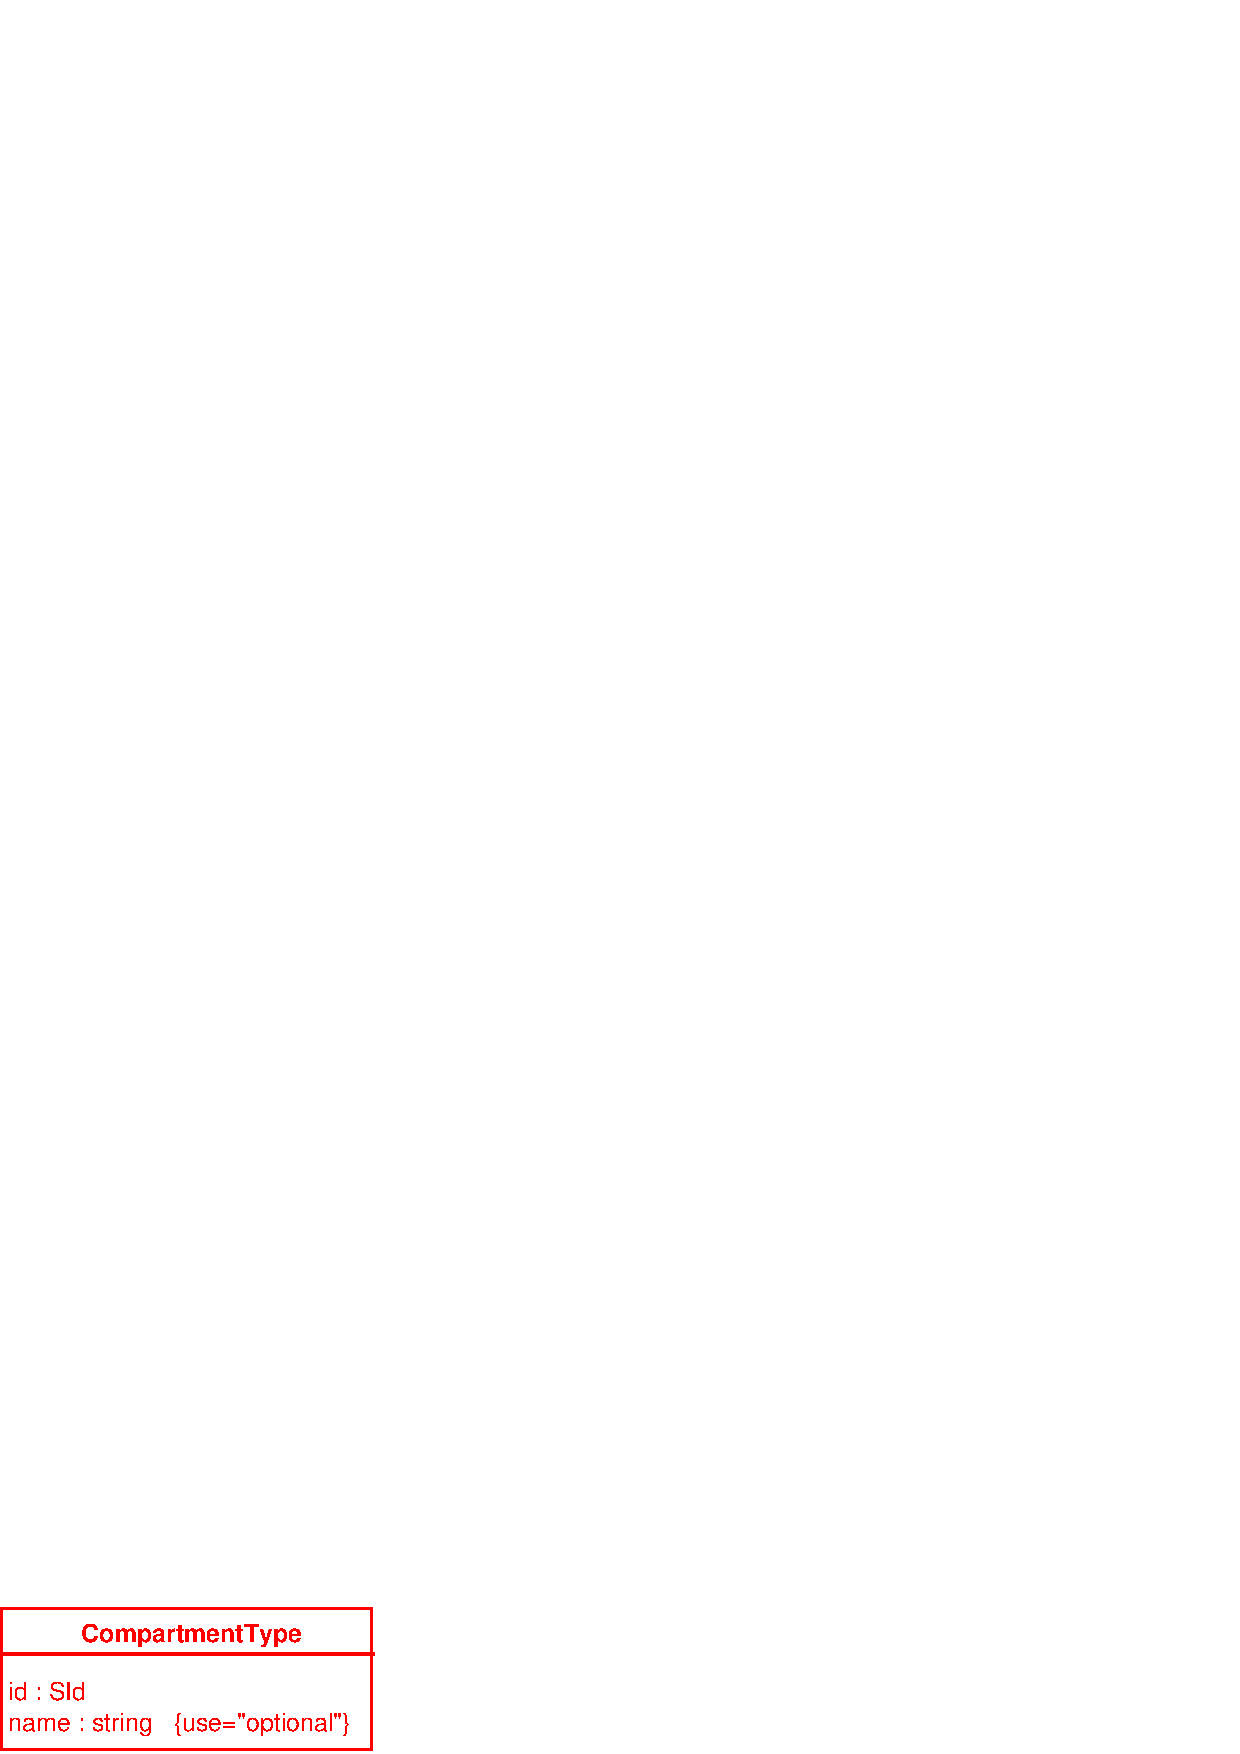
\includegraphics[scale = 0.68]{compartmentType}
  \caption{The definition of \class{CompartmentType}.  Following UML notation,
    additional fields
    that are inherited from a base class, in this case \class{SBase}, are not shown.}
  \label{fig:compartmentType}
  \end{blockChanged}
\end{figure}

In \twotwo, a compartment type only has an identity, and this identity can
only be used to indicate that particular compartments belong to this type.
This may be useful for conveying a modeling intention, such as when a model
contains many identical compartments; without a compartment type construct,
it would be impossible in the language of SBML to indicate that all of the
compartments share an underlying conceptual relationship because each
SBML compartment must be given a unique and separate identity.

Compartment types have no mathematical meaning in SBML---they have no
effect on a model's mathematical interpretation.  Simulators and other
numerical analysis software may ignore \class{CompartmentType} structures
and references to them in a model.

There is no mechanism in SBML for representing hierarchies of
compartment types.  One \class{CompartmentType} structure cannot
be the subtype of another \class{CompartmentType} structure; SBML
provides no means of defining such relationships.


\subsubsection{The \attrib{id} and \attrib{name} Fields}

As with other major structures in SBML, \class{CompartmentType}
has a mandatory field, \attrib{id}, used to give the species type
an identifier. The identifier must be a text string conforming to
the syntax permitted by the \class{SId} data type described in
Section~\ref{sec:id}.  \class{SpeciesType} also has an optional
\attrib{name} field, of type \class{string}.  The \attrib{name}
and \attrib{id} fields \changed{must} be used as described in
Section~\ref{sec:idnameattribs}.


\subsubsection{Examples}

The following partial SBML example illustrates a compartment type used to
relate together many individual compartments in a hypothetical model.

\begin{example}
<model>
    ...
    <listOfCompartmentTypes>
        <compartmentType id="mitochondria"/>
    </listOfCompartmentTypes>
    <listOfCompartments>
        <compartment id="m1" size="0.013" compartmentType="mitochondria" outside="cell"/>
        <compartment id="m2" size="0.013" compartmentType="mitochondria" outside="cell"/>
        <compartment id="m3" size="0.013" compartmentType="mitochondria" outside="cell"/>
        <compartment id="m4" size="0.013" compartmentType="mitochondria" outside="cell"/>
        <compartment id="cell" size="190.0"/>
    </listOfCompartments>
    ...
</model>
\end{example}

\end{blockChanged}


%-----------------------------------------------------------------------------
\subsection{Compartments}
\label{sec:compartments}
%-----------------------------------------------------------------------------
A \emph{compartment} in SBML represents a bounded space in which species
are located.  Compartments do not necessarily have to correspond to actual
structures inside or outside of a cell, although models are often designed
that way.  The definition of \class{Compartment} is shown in
Figure~\vref{fig:compartment}.

\begin{figure}[htb]
  \vspace*{8pt}
  \centering
  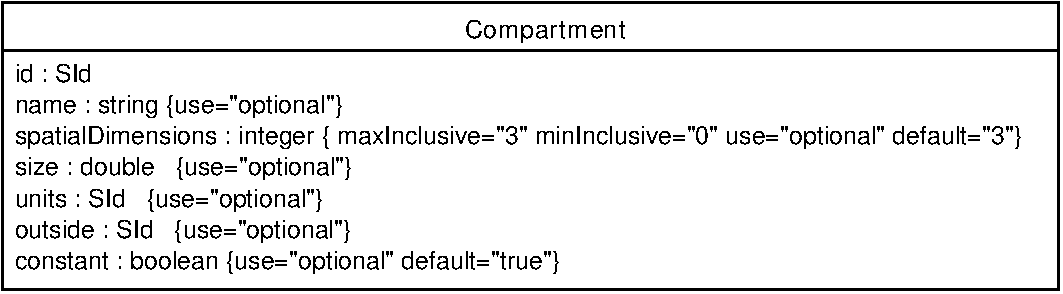
\includegraphics[scale = 0.68]{compartment}
  \caption{The definition of \class{Compartment}.  Following UML notation,
    additional fields
    that are inherited from a base class, in this case \class{SBase}, are not shown.}
  \label{fig:compartment}
\end{figure}

It is worth pointing out that, although compartments are optional in the
overall definition of \class{Model} (see Section~\ref{sec:model}), every
species in an SBML model must be located in a compartment.  This in turn
means that if a model declares any species, the model must also declare at
least one compartment.

\subsubsection{The \attrib{id} and \attrib{name} Fields}

\class{Compartment} has one required field, \attrib{id}, of type
\class{SId}, to give the compartment a unique identifier by which other
parts of an SBML model definition can refer to it.  A compartment can also
have an optional \attrib{name} field of type \class{string}.  Identifiers
and names \changed{must} be used according to the guidelines described in
Section~\ref{sec:idnameattribs}.

\subsubsection{The \attrib{spatialDimensions} Field}

A \class{Compartment} structure has an optional field
\attrib{spatialDimensions}, whose value must be a positive integer
indicating the number of spatial dimensions possessed by the compartment.
The maximum value of \attrib{spatialDimensions} is ``\texttt{3}'', meaning
a three-dimensional structure (a volume).  Other permissible values are
``\texttt{2}'' (for a two-dimensional area), ``\texttt{1}'' (for a
one-dimensional curve), and ``\texttt{0}'' (for a point).  The default value
is ``\texttt{3}''.

\subsubsection{The \attrib{size} Field}
\label{sec:size}

Each compartment has an optional floating-point field named
\attrib{size}, representing the total size of the compartment.  The
\attrib{size} field enables concentrations of species to be calculated in
the absence of geometry information.  Note in particular that in SBML Level~2,
a missing \attrib{size} value does \emph{not} imply that the compartment size is 1.
(This is unlike the definition of compartment \attrib{volume} in SBML
Level~1.)  The \attrib{size} field must not be present if the
\attrib{spatialDimensions} field is has a value of ``\texttt{0}''.
When the \attrib{spatialDimensions} field does not have a value of ``\texttt{0}'',
a missing value for \attrib{size} for a given compartment signifies that the value is
either unknown, \changed{determined by an \class{AssignmentRule} or
  \class{InitialAssignment} structure, not required for analysis,
or is available} from an external data source.

\subsubsection{The \attrib{units} Field}
\label{sec:compartment-units}

The units associated with the compartment's \attrib{size} value
may be explicitly set using the optional field \attrib{units}. The
value chosen for this field must be either one of the base units
from Table~\vref{tab:unitkind}, or the built-in units
``\unit{volume}'', ``\unit{area}'', ``\unit{length}'' or
``\unit{dimensionless}'', or a new unit defined by a unit
definition in the enclosing model.  \changed{The type of units
assigned to the \attrib{units} field must also agree with the
number of spatial dimensions of the compartment; that is, if the chosen
units are not ``\unit{dimensionless}'',  they must be either
units of volume if the value of
\attrib{spatialDimensions} is ``\attribvalue{3}'',
units of area if the value of \attrib{spatialDimensions} is
``\attribvalue{2}'', or units of length
if the value of \attrib{spatialDimensions} is ``\attribvalue{1}''.  If
\attrib{spatialDimensions} is ``\attrib{0}'', the units
associated with the compartment's \attrib{size} can only be
``\unit{dimensionless}''.}

\begin{blockChanged}
The default units depends on the value of the compartment's
\attrib{spatialDimensions} field according to the following rule: for
spatial dimensions of 3, 2, 1 or 0, the compartment has the default units
of \unit{volume}, \unit{area}, \unit{length} and \unit{dimensionless},
respectively.  (See Table~\vref{tab:builtin} and
Table~\vref{tab:unitkind}.)
\end{blockChanged}

The units of the compartment size, as defined by the \attrib{units} field,
are used in the following ways:
\begin{itemize}

\item The value of the \attrib{units} field is used as the units of the \attrib{size}
  field of the
  compartment structure (see Section~\ref{sec:size}).

\item The value of the \attrib{units} field is used as the units of the
  compartment identifier when it appears as a numerical quantity in a mathematical
  formula expressed in MathML (discussed in Section~\ref{sec:ci-token}).

\item The value of the \attrib{units} field is used as the units of the
  \attrib{math} field \changed{provided on
  \class{AssignmentRule} and \class{InitialAssignment} structures
  for setting a compartment's size}
  (see Section~\ref{sec:assignmentrule}).

\item In a \class{RateRule} structure that
  sets the rate of change of the compartment's size
  (Section~\ref{sec:raterule}), the units on the rule's \attrib{math} field are
  those in the compartment's \attrib{units} field divided by the default
  \quantity{time} units.  (In other words, the units for the rate of change
  of compartment size are \quantity{compartment size}/\quantity{time} units.)
\end{itemize}

\subsubsection{The \attrib{constant} Field}
\label{sec:compartment-constant}

A \class{Compartment} also has an optional boolean field called
\attrib{constant} that indicates whether the compartment's size
stays constant or can vary during a simulation.  A value of
``\attribvalue{false}'' indicates the compartment's size can be
determined by rules (see Section~\ref{sec:rules}), and the value
of the \attrib{size} field should be taken as being the initial
size of the compartment.  The default value for the
\attrib{constant} field is ``\attribvalue{true}'' because in the
most common modeling scenarios at the time of this writing,
compartment sizes remain constant. The \attrib{constant} field
must default to or be set to ``\attribvalue{true}'' if the
\attrib{spatialDimensions} field is 0.

\subsubsection{The \attrib{outside} Field}
\label{sec:compartment-outside}

The optional field \attrib{outside} of type \class{SId} can be
used to express containment relationships between compartments. If
present, the value of \attrib{outside} for a given compartment
must be \changed{the \attrib{id} field value of another
compartment which encloses it}, or in other words, the compartment
that is ``outside'' of it. This enables the representation of
simple topological relationships between compartments, for those
simulation systems that can make use of the information (e.g., for
drawing simple diagrams of compartments).

\changed{The directed graph formed by representing
\class{Compartment} structures as vertexes and the \class{outside}
attribute values as edges must be acyclic.  If this condition were not
imposed, a model could contain a \class{Compartment} that
was contained inside itself.}

Although containment relationships are partly taken into account by the
compartmental localization of reactants and products, it is not always
possible to determine purely from the reaction equations whether one
compartment is meant to be located within another.  In the absence of a
value for \attrib{outside}, compartment definitions in SBML Level~2 do not
have any implied spatial relationships between each other.  For many
modeling applications, the transfer of substances described by the
reactions in a model sufficiently express the relationships between the
compartments.  (As discussed in Section~\ref{sec:level-3}, we expect that
SBML Level~3 will introduce the ability to define geometries and spatial
qualities.)

\begin{blockChanged}
\subsubsection{The \attrib{compartmentType} Field}
\label{sec:compartment-compartment-type}

Each compartment in a model may optionally be designated as
belonging to a particular compartment type. The optional field
\attrib{compartmentType} of type \class{SId} is used identify the
compartment type represented by the \class{Compartment} structure.
The field's value must be the identifier of an existing
\class{CompartmentType} structure.  If the
\attrib{compartmentType} field is not present on a particular
compartment definition, a unique virtual compartment type is assumed for
that compartment, and no other compartment can belong to that
compartment type.

The values of \class{compartmentType} attributes on compartments
have no effect on the numerical interpretation of a model.
Simulators and other numerical analysis software may ignore
\class{compartmentType} attributes.

\end{blockChanged}


\subsubsection{Examples}

The following example illustrates two
compartments in an abbreviated SBML example of a model definition:

\begin{example}
<model>
    ...
    <listOfCompartments>
        <compartment id="cytosol" size="2.5"/>
        <compartment id="mitochondria" size="0.3"/>
    </listOfCompartments>
    ...
</model>

\end{example}

The following is an example of using \attrib{outside} to model a cell
membrane.  To express that a compartment named B has a membrane that is
modeled as another compartment M, which in turn is located within another
compartment A, one would write:

\begin{example}
<model>
    ...
    <listOfCompartments>
        <compartment id="A"/>
        <compartment id="M" spatialDimensions="2" outside="A"/>
        <compartment id="B" outside="M"/>
    </listOfCompartments>
    ...
</model>

\end{example}


%-----------------------------------------------------------------------------
\begin{blockChanged}
\subsection{SpeciesType}
\label{sec:speciesType}
%-----------------------------------------------------------------------------

The term \emph{species type} refers to chemical entities
independent of location.  These include simple ions (e.g.,
protons, calcium), simple molecules (e.g., glucose, ATP), large
molecules (e.g., RNA, polysaccharides, and proteins), and others.
The \class{SpeciesType} data structure is intended to represent
these entities.  Its definition is shown in
Figure~\vref{fig:speciesType}.

\begin{figure}[htb]
  \begin{blockChanged}
  \centering
  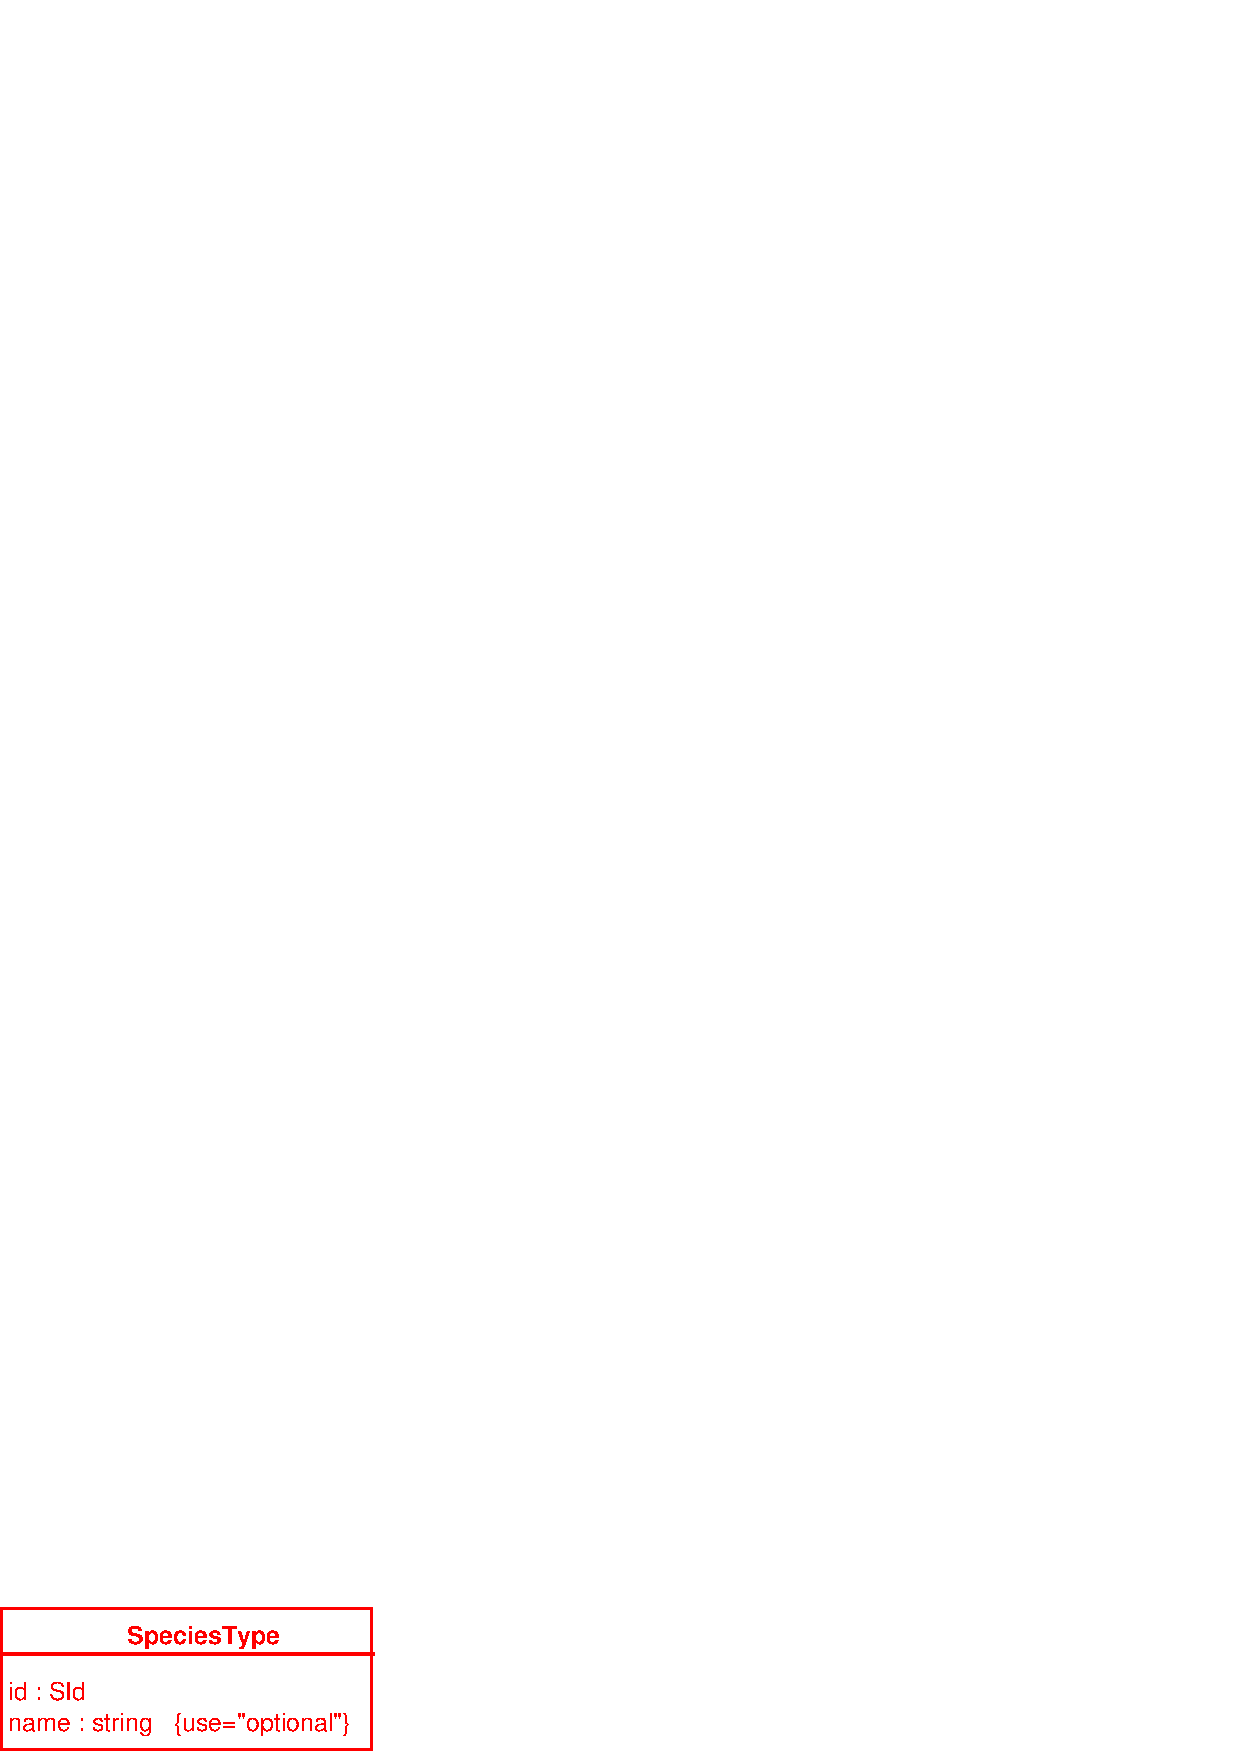
\includegraphics[scale = 0.68]{speciesType}
  \caption{The definition of \class{SpeciesType}.  Following UML notation,
    additional fields
    that are inherited from a base class, in this case \class{SBase}, are not shown.}
  \label{fig:speciesType}
  \end{blockChanged}
\end{figure}

\class{SpeciesType} structures are included in SBML to enable
\class{Species} (Section~\ref{sec:species}) of the same type to
be related together.  It is a conceptual construct; the
existence of \class{SpeciesType} structures in a model has no
effect on the model's numerical interpretation.  Except for the
requirement for uniqueness of species/species type combinations
located in compartments (described in
Section~\ref{sec:species-species-type}), simulators and other
numerical analysis software may ignore \class{SpeciesType}
structures and references to them in a model.

There is no mechanism in SBML for representing hierarchies of
species types.  One \class{SpeciesType} structure cannot be the
subtype of another \class{SpeciesType} structure; SBML provides
no means of defining such relationships.

An example of a model that is encoded using \class{SpeciesType}
structures is shown in Section~\ref{sec:speciesType-eg}.

\subsubsection{The \attrib{id} and \attrib{name} Fields}

As with other major structures in SBML, \class{SpeciesType} has a
mandatory field, \attrib{id}, used to give the species type an
identifier.  The identifier must be a text string conforming to
the syntax permitted by the \class{SId} data type described in
Section~\ref{sec:id}.  \class{SpeciesType} also has an optional
\attrib{name} field, of type \class{string}.  The \attrib{name}
and \attrib{id} fields \changed{must} be used as described in
Section~\ref{sec:idnameattribs}.

\subsubsection{Example}

The following XML fragment is an example of two
\class{SpeciesType} structures embedded in an SBML model.

\begin{example}
<model>
    ...
    <listOfSpeciesTypes>
        <speciesType id="Glucose"/>
        <speciesType id="Glucose_6_P"/>
    </listOfSpeciesTypes>
    ...
</model>
\end{example}

\end{blockChanged}


%-----------------------------------------------------------------------------
\subsection{Species}
\label{sec:species}
%-----------------------------------------------------------------------------

\changed{A \emph{species} refers to a pool of chemical
entities of a specific \emph{species type} that take part in
reactions and are located in a specific \emph{compartment}.
The \class{Species} data
structure is intended to represent these pools.}   Its definition
is shown in Figure~\vref{fig:species}.

\begin{figure}[htb]
  \centering
  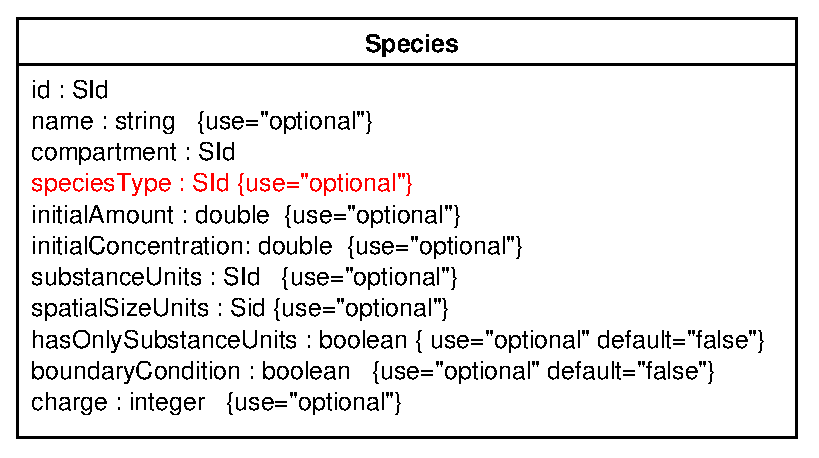
\includegraphics[scale = 0.68]{specie}
  \caption{The definition of \class{Species}.  Following UML notation,
    additional fields
    that are inherited from a base class, in this case \class{SBase}, are not shown.}
  \label{fig:species}
\end{figure}

\begin{blockChanged}
Although the exact definition of \class{Species} given here has
changed from the definition in the specification of SBML Level~2
Version~1 (e.g., through the introduction of species types), the
concept represented by \class{Species} remains the same.
\end{blockChanged}


\subsubsection{The \attrib{id} and \attrib{name} Fields}

As with other major structures in SBML, \class{Species} has a mandatory
field, \attrib{id}, used to give the species an identifier.  The identifier
must be a text string conforming to the syntax permitted by the \class{SId}
data type described in Section~\ref{sec:id}.  \class{Species} also has an
optional \attrib{name} field, of type \class{string}.  The \attrib{name}
and \attrib{id} fields \changed{must} be used as described in
Section~\ref{sec:idnameattribs}.

\subsubsection{The \attrib{compartment} Field}
\label{sec:species-compartment}

The required field \attrib{compartment}, also of type \class{SId},
is used to identify the compartment in which the species is
located.  The field's value must be the identifier of an existing
\class{Compartment} structure.  It is important to note that there
is no default value for the \attrib{compartment} field on
\class{Species}; every species in an SBML model must be assigned a
compartment, and consequently, a model must define at least one
compartment if that model contains any species.

\begin{blockChanged}
\subsubsection{The \attrib{speciesType} Field}
\label{sec:species-species-type}

Each species in a model may optionally be designated as
belonging to a particular species type.
The optional field \attrib{speciesType} of type \class{SId} is used
identify the species type of the chemical entities that make up
the pool represented by the \class{Species} structure. The field's
value must be the identifier of an existing \class{SpeciesType}
structure.  If the \attrib{speciesType} field is not present on
a particular species definition, it means the
pool contains chemical entities of a type unique to that pool;
in effect, a virtual species type is assumed for that species,
and no other species can belong to that species type.

There can be only one species of a given species type in any
given compartment of a model.  More specifically, for all
\class{Species} structures having a
value for the \attrib{speciesType} field, the pair
\begin{center}
(\attrib{speciesType} field value, \attrib{compartment} field value)
\end{center}
must be unique across the set of all \class{Species} structures
in a model.

The value of \class{speciesType} attributes on species have no
effect on the numerical interpretation of a model. Simulators
and other numerical analysis software may ignore
\class{speciesType} attributes.

\end{blockChanged}

\subsubsection{The \attrib{initialAmount} and \attrib{initialConcentration} Fields}
\label{sec:initialAmount}

The optional fields \attrib{initialAmount} and
\attrib{initialConcentration}, both having a data type of
\class{double}, are used to set the initial quantity of the
species in the named compartment.  These fields are mutually
exclusive; i.e., \emph{only one} can have a value on any given
instance of a \class{Species} structure.  \changed{Also,
\attrib{initialConcentration} must not have a value if the
species' compartment has a \attrib{spatialDimensions} value of
``\texttt{0}''}. Missing \attrib{initialAmount} or
\attrib{initialConcentration} values implies that their values are
either unknown, set by an \changed{\class{AssignmentRule} or
  \class{InitialAssignment}} structure, not required for
analysis, or available from an external data source.

The units of the value in the \attrib{initialAmount} field are
set by the \attrib{substanceUnits} field of the species
structure.  \changed{The units of the value in the
\attrib{initialConcentration} field are
\quantity{substance}/\quantity{size} units (i.e.,
\quantity{concentration}).  The units of \quantity{substance}
are those defined in the \attrib{substanceUnits}, and the
\quantity{size} units are those given in the
\attrib{spatialSizeUnits} field as described in the next
subsection.}

\subsubsection{The \attrib{substanceUnits}, \attrib{spatialSizeUnits} and
    \attrib{hasOnlySubstanceUnits} Fields}
\label{sec:species-units}

The units associated with a species' quantity, referred to as the
\emph{units of the species}, are determined via the
optional fields \attrib{substanceUnits}, \attrib{spatialSizeUnits} and
\attrib{hasOnlySubstanceUnits}.

\attrib{hasOnlySubstanceUnits} is a boolean field which defaults
to ``\attribvalue{false}''. The \emph{units of the species} are of
the form \quantity{substance}/\quantity{size} units (i.e.,
\quantity{concentration} units, using a broad definition of
concentration) if the compartment's \attrib{spatialDimensions} is
non-zero and \attrib{hasOnlySubstanceUnits} has the value
``\attribvalue{false}''. The \emph{units of the species} are of
the form \quantity{substance} if \attrib{spatialDimensions} is
zero or \attrib{hasOnlySubstanceUnits} has the value
``\attribvalue{true}''.  \changed{The possible values of
\emph{units of the species} are summarized in
Table~\ref{tab:speciesunits}.}  The units of \quantity{substance}
are those defined in the \attrib{substanceUnits}, and the
\quantity{size} units are those given in the
\attrib{spatialSizeUnits} field.

\begin{table}[ht]
\begin{blockChanged}
  \vspace*{8pt} \centering
  \small
  \begin{tabular}{lll}
    \toprule
    \textbf{value of} &
    \textbf{\emph{units of the species} when} &
    \textbf{\emph{units of the species} when}\\
    \textbf{\attrib{hasOnlySubstanceUnits}}&
    \textbf{Spatial Dimensions is greater than 0} &
    \textbf{Spatial Dimensions is 0}\\
    \midrule
    \texttt{false} (default) & $substance/size$ & $substance$ \\
    \texttt{true} & $substance$ & $substance$ \\
    \bottomrule
  \end{tabular}
  \caption{How to interpret the value the \attrib{hasOnlySubstanceUnits}
  field of the \class{Species} structure.}
  \label{tab:speciesunits}
\end{blockChanged}
\end{table}

For both \attrib{substanceUnits} and \attrib{spatialSizeUnits},
the value chosen must be either a base unit from
Table~\vref{tab:unitkind}, a built-in unit from
Table~\vref{tab:builtin}, or a new unit defined by a unit
definition in the enclosing model. \changed{The chosen units for
\attrib{substanceUnits} must be be \unit{dimensionless},
\unit{kilogram}, \unit{mole}, \unit{item}, or units derived from these}. The
\attrib{substanceUnits} field defaults to the the built-in unit
``\attrib{substance}'' shown in Table~\vref{tab:builtin}.

The type of units assigned to the \attrib{spatialSizeUnits} field
must agree with the number of spatial dimensions of the species'
compartment.   \changed{Specifically, they must be units of volume
or ``\unit{dimensionless}'' if the value of the compartment's
\attrib{spatialDimensions} is ``\attribvalue{3}''; they must be
units of area or ``\unit{dimensionless}'' if the value of
\attrib{spatialDimensions} is ``\attribvalue{2}''; and they must
be units of length or ``\unit{dimensionless}'' if the value of
\attrib{spatialDimensions} is ``\attribvalue{1}''.} The
\attrib{spatialSizeUnits} field must not have a value if
\attrib{spatialDimensions} on the compartment has a value of
``\attribvalue{0}'', or if the species'
\attrib{hasOnlySubstanceUnits} field has a value of
``\attribvalue{true}''. The default value of the
\attrib{spatialSizeUnits} is the value of the \attrib{units} field
of the species' compartment.

\begin{blockChanged}
The \emph{units of the species} are used in the following ways:

\begin{itemize}
\item The
  species identifier has these units when it appears as a numerical quantity
  in a mathematical formula expressed in MathML
  (discussed in Section~\ref{sec:ci-token}).

\item The
   \attrib{math} field of
  \class{AssignmentRule} \changed{and \class{InitialAssignment} structures}
  determining the species' quantity
  (see Section~\ref{sec:assignmentrule}) has these units.

\item In \class{RateRule} structures that
  set the rate of change of the species' quantity
  (Section~\ref{sec:raterule}), the units on the rule's \attrib{math} field are
  the \emph{units of the species} divided by the built-in
  \quantity{time} units.

\end{itemize}
\end{blockChanged}

\subsubsection{The \attrib{constant} and \attrib{boundaryCondition} Fields}
\label{sec:species-constant}

The \class{Species} structure has an optional boolean field named
\attrib{constant} used to indicate whether the concentration of
that species can vary during a simulation.  The default value is
``\attribvalue{false}'', indicating that the species' concentration can be
determined by reactions, rules and initial assignments.

Another optional field defined for \class{Species} is
\attrib{boundaryCondition}.  By default, when a species is a product or
reactant of one or more reactions, its concentration is determined by those
reactions.  In SBML, it is possible to indicate that a given species'
concentration is \emph{not} determined by the set of reactions even when
that species occurs as a product or reactant; i.e., the species is on the
\emph{boundary} of the reaction system but is a component of the rest of
the model.  The boolean field \attrib{boundaryCondition} can be used to
indicate this.  The value of the field defaults to ``\attribvalue{false}'',
indicating the species \emph{is} part of the reaction
system.  Table~\ref{tab:specieattrib} shows how to interpret the combined
values of the \attrib{boundaryCondition} and \attrib{constant} fields.  In
practice, a \attrib{boundaryCondition} value of ``\attribvalue{true}''
means a differential equation derived from the reaction definitions
should not be generated for the species.  The example model in
section~\ref{sec:constantspecieseg} contains all four possible combinations
of the \attrib{boundaryCondition} and \attrib{constant} fields on
\class{species} elements.  Section~\ref{sec:odeeg} contains a translation into
ODEs of a model which uses \attrib{boundaryCondition} and \attrib{constant} fields.

\begin{table}[ht]
  \vspace*{8pt} \centering
  \small
  \begin{tabular}{lllll}
    \toprule
    \textbf{\attrib{constant}} & \textbf{\attrib{boundaryCondition}} &
    \textbf{can have} & \textbf{can be} & \textbf{concentration} \\
    \textbf{value} & \textbf{value} & \textbf{assignment} & \textbf{reactant or} & \textbf{is changed by} \\
    & & \textbf{or rate rule} & \textbf{product}\\
    \midrule
    true & true & no & yes & never changes\\
    false & true & yes & yes & rule \\
    true & false & no & no & never changes \\
    false & false & yes & yes & reactions or rule but not both \\
    \bottomrule
  \end{tabular}
  \caption{How to interpret the values of the \attrib{constant} and
    \attrib{boundaryCondition} fields of the \class{Species} structure.}
  \label{tab:specieattrib}
\end{table}

\subsubsection{The \attrib{charge} Field}
\label{sec:charge}

The optional field \attrib{charge} takes an integer indicating the
charge on the species (in terms of electrons, not the SI unit
coulombs). This may be useful when the species is a charged ion
such as calcium ($\text{Ca}^{2+}$).  \changed{The \attrib{charge}
field is deprecated in SBML Level~2 Version~2: parsers are free to
ignore this field and generators do not need to create this
field.}

\subsubsection{Example}

The following example shows two species definitions within an
abbreviated SBML model definition.  The example shows that species
are listed under the heading \attrib{listOfSpecies} in the model:

\begin{example}
<model>
    ...
    <listOfSpecies>
        <species id="Glucose" compartment="cell" initialConcentration="4"/>
        <species id="Glucose_6_P" compartment="cell" initialConcentration="0.75"/>
    </listOfSpecies>
    ...
</model>
\end{example}


%-----------------------------------------------------------------------------
\subsection{Parameters}
\label{sec:parameters}
%-----------------------------------------------------------------------------

A \class{Parameter} structure is used to declare a variable for use in
mathematical formulas in an SBML model definition.  By default, parameters
have constant value for the duration of a simulation and for this reason
are called ``parameters'' instead of variables in SBML.  The definition of
\class{Parameter} is shown in Figure~\vref{fig:parameter}.

\begin{figure}[htb]
  \vspace*{6pt}
  \centering
  
\includegraphics[scale = 0.68]{parameter}
  \caption{The definition of \class{Parameter}. Following UML notation, additional
    fields
    that are inherited from a base class, in this case \class{SBase}, are not shown.}
  \label{fig:parameter}
\end{figure}

\begin{blockChanged}
Parameters can be defined in two places in SBML: in lists of parameters
defined at the top level in a \class{Model} structure, and within
individual reaction definitions (as described in
Section~\ref{sec:reactions}).  Parameters defined at the top level are
\emph{global} to the whole model; parameters that are defined within a
reaction are local to the particular reaction and (within that reaction)
\emph{override} any global parameters having the same names (See
Section~\ref{sec:namespaces} for further details).
\end{blockChanged}


\subsubsection{The \attrib{id} and \attrib{name} Fields}

\class{Parameter} has one required field, \attrib{id}, of type \class{SId},
to give the parameter a unique identifier by which other parts of an SBML
model definition can refer to it.  A parameter can also have an optional
\attrib{name} field of type \class{string}.  Identifiers and names \changed{must}
be used according to the guidelines described in
Section~\ref{sec:idnameattribs}.

\subsubsection{The \attrib{value} Field}

\changed{The optional field \attrib{value} determines the value
(of type \class{double}) assigned to the identifer.  A missing
\attrib{value} implies that the \attrib{value} is either (a)
unknown; (b) determined by an \class{AssignmentRule} or
\class{InitalAssignment} structure; (c) not required for analysis;
or (d) available from an external data source. If the parameter is
not constant then the \attrib{value} field contains the initial
value.}

\subsubsection{The \attrib{units} Field}
\label{sec:parameter-units}

The units associated with the value of the parameter are specified
by the field \attrib{units}.  \changed{These units are relevant
when the parameter identifier appears in: (a)
\class{AssignmentRule} and \class{InitialAssignment} structures
setting the value of the parameter; and (b) MathML expressions.} A
\class{RateRule} structure that may determine the value of the
parameter has units \quantity{parameter
  units}/\quantity{time}, where \quantity{parameter units} are the units
assigned to the parameter and \quantity{time} is the built-in \unit{time}
units.  The value assigned to the parameter's \attrib{units} field must
be chosen from one of the following possibilities: one of the base unit
names from Table~\vref{tab:unitkind}; one of the built-in unit names
appearing in first column of Table~\vref{tab:builtin}; or the name of a
new unit defined in the list of unit definitions in the enclosing
\class{Model} structure.  There are no constraints on which units can be
chosen from these sets.  There are no default units for parameters.

\subsubsection{The \attrib{constant} Field}

The \class{Parameter} structure has an optional boolean field named
\attrib{constant} which indicates whether the parameter's value can vary
during a simulation.  The field's default value is ``\attribvalue{true}'';
a value of ``\attribvalue{false}'' indicates the parameter's value can
be changed by rules (see Section~\ref{sec:rules}) and the
\attrib{value} is actually intended to be the initial value of the
parameter.

\begin{blockChanged}
Parameters local to a reaction (i.e., those defined within a
\class{Reaction}'s \class{KineticLaw} structure, as described in
Section~\ref{subsec:kinetic-law}) cannot be changed by rules and
therefore are implicitly always constant; thus, parameter
definitions within \class{Reaction} structures should \emph{not}
have their \attrib{constant} field set to ``\attribvalue{false}'';
\end{blockChanged}

\begin{blockChanged}

\subsubsection{The \attrib{sboTerm} Field}

The \class{Parameter} structure has an optional \class{SBOTerm}
field, \attrib{sboTerm} (see Section~\ref{sec:sboTerm}).  This
field when present must contain an Systems Biology Ontology
(SBO)\sboref term identifier referring to a parameter SBO term,
that is a term derived from \sboparameter.  The
\class{SpeciesReference} structure should have a `is a'
relationship with the SBO term. The SBO term chosen should be the
most precise (narrow) term that captures the role of the given
parameter.

\end{blockChanged}

\subsubsection{Example}

The following is an example of parameters defined at the \class{Model} level:

\begin{example}
<model>
    ...
    <listOfParameters>
        <parameter id="tau1" value="2.3" units="second"/>
        <parameter id="Km1" value="10.7" units="\changed{moleperlitre}"/>
    </listOfParameters>
    ...
</model>
\end{example}


\begin{blockChanged}
%-----------------------------------------------------------------------------
\subsection{Initial Assignments}
\label{sec:initialAssignment}
%-----------------------------------------------------------------------------

An \emph{Initial Assignment} enables the calculation of the value
of a constant or the initial value of a variable from the values
of other constants or the initial values of other variables.  An
\class{InitialAssignment} structure consists of two fields,
\attrib{symbol} and \attrib{math}, as shown in
Figure~\vref{fig:initialAssignment}.  The \attrib{symbol} field
has type \class{SId} and contains the value of an
\attrib{id} field defined for a \class{compartment},
\class{species} or \class{parameter} elsewhere in the model. The
\class{InitialAssignment} structure assigns the initial value of
the constant or variable referred to by the \attrib{symbol} field.
The \attrib{math} field contains a MathML expression that is used
to calculate the value of the constant or the initial value of the
variable.

\begin{figure}[htb]
  \begin{blockChanged}
  \centering
  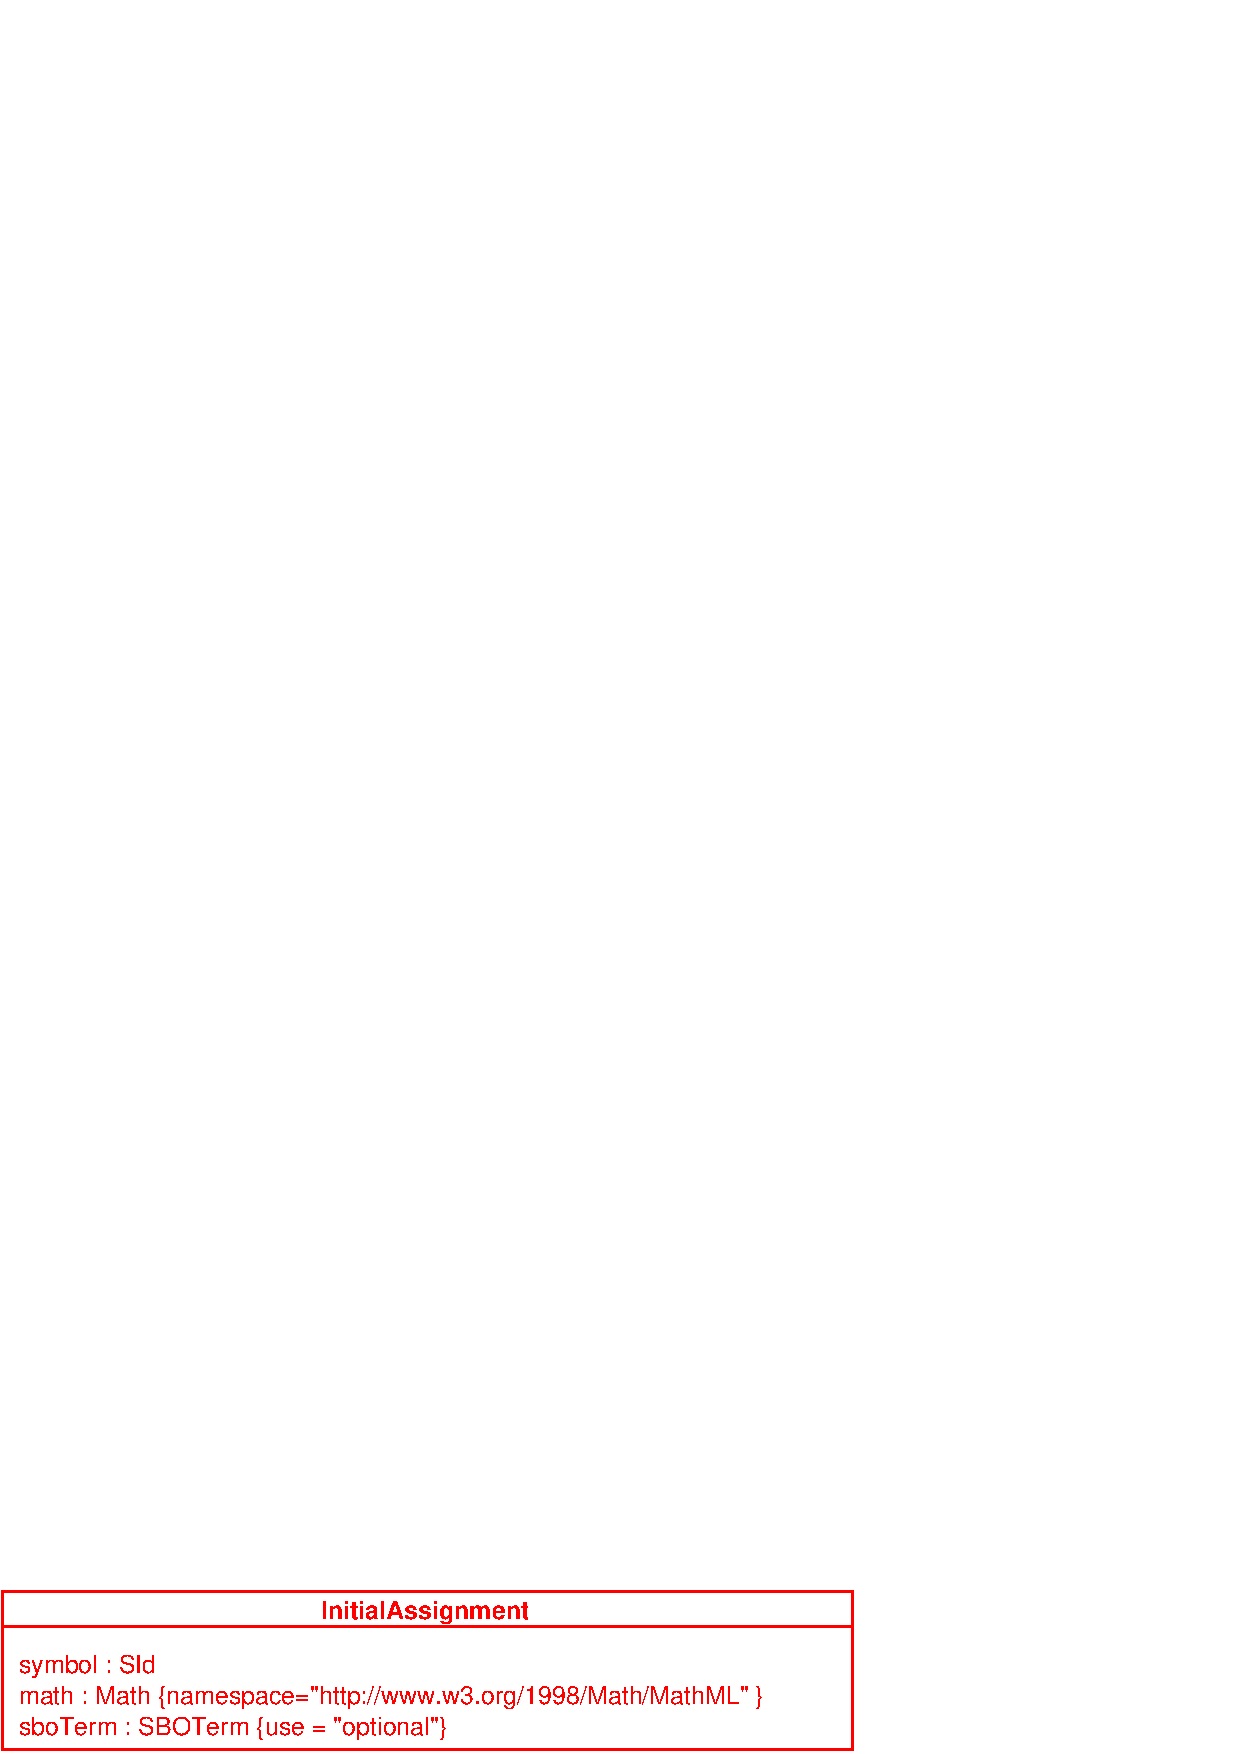
\includegraphics[scale = 0.68]{initialAssignment}
  \caption{The definition of \class{InitialAssignment}.
    Following UML notation fields
    that are inherited from a base class are not shown.}
  \label{fig:initialAssignment}
  \end{blockChanged}
\end{figure}

The value calculated by an \class{InitialAssignment} structure
overrides the value associated with the given symbol by the
structure declaring the symbol.  Parsers must ignore the value
associated with a symbol by the structure declaring the symbol if
an \class{InitialAssignment} structure exists which has a
\attrib{symbol} field value equal to the symbol. This does not
mean that a structure declaring a symbol can be omitted if there
is an \class{InitialAssignment} structure for that symbol. For
example, there must be a \texttt{Parameter} structure for a given
parameter if there is a \class{InitialAssignment} structure for
that parameter. Any pair of \class{AssignmentRule} and a
\class{InitialAssignment} rules cannot have the same
\attrib{variable} attribute value.

Unlike an \class{AssignmentRule} structure, an
\class{InitialAssignment} structure only applies at the start of
simulated time and can set the value of a constant. In all cases,
as would be expected, the units of the formula in the
\attrib{math} field are identical to the units associated with the
identifier given in the \attrib{symbol} field, when that variable
appears in other formulas.

The effects of an \class{InitialAssignment} structure are in
general terms the same, but differ in the precise details
depending on the type of variable being set:

\begin{itemize}

\item \emph{In the case of a species}, an
\class{InitialAssignment} sets the
  referenced species' initial quantity (\quantity{concentration} or
  \quantity{amount of substance})
  to the value determined by the formula
  in \attrib{math}.  (See Section~\ref{sec:species-units} for an
  explanation of how the units of the species' quantity are determined.)

\item \emph{In the case of a compartment}, an
\class{InitialAssignment} sets
  the referenced compartment's initial size to the size determined by the formula
  in \attrib{math}.  The overall units of the formula are the units
  specified for the size of the compartment identified by the value of the
  \class{InitialAssignment}'s \attrib{symbol} field.  (See
  Section~\ref{sec:compartment-units} for an explanation of how the units of the
  compartment's size are determined.)

\item \emph{In the case of a parameter}, an
\class{InitialAssignment} sets the
  referenced parameter's initial value to that determined by the formula in
  \attrib{math}.  The overall units of the formula are the units
  defined for the parameter identified by the value of the
  \class{InitialAssignment}'s \attrib{variable} field.  (See
  Section~\ref{sec:parameter-units} for an explanation of how the units of the
  parameter are determined.)

\end{itemize}

An \class{InitialAssignment} structure for a given identifier
overrides the initial value assigned to that identifier; i.e., the
initial value should be ignored. This does not mean that a
structure declaring an identifier can be omitted if there is an
\class{InitialAssignment} structure for that identifier.  For
example, there must be a \texttt{Parameter} structure for a given
parameter if there is a \class{InitialAssignment} structure for
that parameter.

The ordering of \class{InitialAssignment} structures is not
significant.
The combined set of \class{InitialAssignment},
\class{AssignmentRule} and \class{KineticLaw} structures form a
set of assignment statements that should be considered as a whole.
This set should not contain more than one assignment for the same
symbol: a model should not contain either: (a) two or more
\class{InitialAssignment} structures with the same \attrib{symbol}
field value; and (b) an \class{InitialAssignment} structure with a
\attrib{symbol} field value which is the same as a
\class{AssignmentRule} \attrib{variable} field value. The combined
set of assignment statements should not contain algebraic loops: a
chain of dependency between these statements should terminate.
(More formally, consider the directed graph of assignment statements
where nodes are rules and directed arcs exist for each occurrence
of a symbol in a assignment statement \attrib{math} field.  The
directed arcs in this graph start from the statement assigning the symbol and
end at the statement that contains the symbol in their math
fields. Such a graph must be acyclic.) Examples of valid and
invalid set of assignment statements are given in
Section~\ref{sec:ruleconstraints}.

\subsubsection{The \attrib{sboTerm} Field}

The \class{InitialAssignment} structure has an optional
\class{SBOTerm} field, \attrib{sboTerm} (see
Section~\ref{sec:sboTerm}).  This field when present must contain
an Systems Biology Ontology (SBO)\sboref term identifier.  The
\class{InitialAssignment} structure should have a `is a'
relationship with the SBO term. The SBO term chosen should be the
most precise (narrow) term that matches the form of the
\class{InitialAssignment}.

\subsubsection{Example}

The following example shows how the species $x$ can assigned the
initial value $2y$:

\begin{example}
<model>
    <listOfSpecies>
        <species id="x" initialConcentration="5"/>
    </listOfSpecies>
    ...
    <listOfInitialAssignments>
        <initialAssignment symbol="x">
            <math xmlns="http://www.w3.org/1998/Math/MathML">
                <apply>
                    <times/>
                    <ci> y </ci>
                    <cn> 2 </cn>
                </apply>
            </math>
        </initialAssignment>
    </listOfInitialAssignments>
    ...
</model>
\end{example}

\end{blockChanged}

%-----------------------------------------------------------------------------
\subsection{Rules}
\label{sec:rules}
%-----------------------------------------------------------------------------

\emph{Rules} provide a way to create constraints on variables for
cases in which the constraints cannot be expressed using reactions
(Section~\ref{sec:reactions}) nor the assignment of an initial
value to a component in a model.  There are two orthogonal
dimensions by which rules can be described.  First, there are
three different possible functional forms, corresponding to the
following three general cases (where $x$ is a variable, $f$ is
some arbitrary function returning a numeric result, $V$ is a
vector of variables that does not include $x$, and $W$ is a vector
of variables that may include $x$):

\begin{center}
\begin{tabular}{rll}
\emph{Algebraic}    & left-hand side is zero:             & $0 = f(W)$\\
\emph{Assignment}  & left-hand side is a scalar:         & $x = f(V)$\\
\emph{Rate}         & left-hand side is a rate-of-change: & $dx/dt = f(W)$\\
\end{tabular}
\end{center}


The second dimension concerns the role of variable $x$ in the
equations above: $x$ can be the identifier of a compartment (to
set its size), a species (to set its concentration), or a
parameter (to set its value).

In their general form given above, there is little to distinguish between
\emph{assignment} and \emph{algebraic} rules.  They are treated as separate
cases for the following reasons:
\begin{itemize}

\item \emph{Assignment} rules can simply be evaluated to calculate intermediate
  values for use in numerical methods;

\item Some simulators do not contain numerical solvers capable of solving
  unconstrained \emph{algebraic} equations;

\item Those simulators that \emph{can} solve these \emph{algebraic}
  equations make a distinction between the different categories listed
  above; and

\item Some specialized numerical analyses of models may only be applicable to
  models that do not contain \emph{algebraic} rules.
\end{itemize}

The approach taken to covering these cases in SBML is to define an
abstract \class{Rule} structure containing only one field,
\attrib{math}, to hold the right-hand side expression, then to
derive subtypes of \class{Rule} that add fields to distinguish the
cases of algebraic, assignment and rate rules.
Figure~\vref{fig:rules} gives the definitions of \class{Rule} and
the subtypes derived from it.  The figure shows there are four
subtypes, \class{AlgebraicRule}, \class{AssignmentRule} and
\class{RateRule} derived directly from \class{Rule}. These
correspond to the cases \emph{Algebraic}, \emph{Assignment}, and
\emph{Rate} described above respectively.

\begin{figure}[htb]
  \vspace*{-5pt}
  \centering
  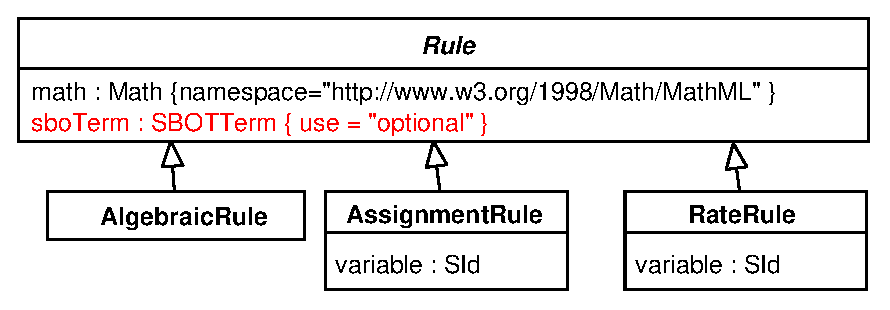
\includegraphics[scale = 0.68]{rule}
  \caption{The definition of \class{Rule} and derived types.
    Following UML notation fields
    that are inherited from a base class are not shown.}
  \label{fig:rules}
\end{figure}

\changed{The \class{Rule} structure has an optional
\class{SBOTerm} field, \attrib{sboTerm} (see
Section~\ref{sec:sboTerm}).  This field when present must contain
an Systems Biology Ontology (SBO)~\sboref term identifier.  The
\attrib{sboTerm} field should contain a SBO term identifier
referring to an actual SBO Term. The \class{Rule} structure should
have a `is a' relationship with the SBO term. The SBO term chosen
should be the most precise (narrow) term that matches the form of
the \class{Rule}.}

\subsubsection{\class{AlgebraicRule}}
\label{sec:algebraicrule}

The rule type \class{AlgebraicRule} is used to express equations that are
neither assignments of model variables nor rates of change.
\class{AlgebraicRule} does not add any fields to the basic \class{Rule};
its role is simply to distinguish this case from the other cases.  An
 example of the use of \class{AlgebraicRule} structures is given in
Section~\ref{sec:algeraiceg}.

\subsubsection{\class{AssignmentRule}}
\label{sec:assignmentrule}

The rule type \class{AssignmentRule} is used to express equations
that set the values of variables.  The left-hand side (the
\attrib{variable} field) of an assignment rule can refer to the
identifier of a species, compartment, or parameter \changed{(but
not a reaction)}.  Two or more \class{RateRule} or
\class{AssignmentRule} structures cannot have the same left-hand
side or \attrib{variable} field value in an SBML model definition.
In all cases, as would be expected, the units of the formula
representing the right hand side, the \attrib{math} field, are
identical to the units associated with the left hand side, the
\attrib{variable} field, when that variable appears in other
formulas.

The effects of an \class{AssignmentRule} structure are in general terms
the same, but differ in the precise details depending on the type of variable
being set:

\begin{itemize}

\item \emph{In the case of a species}, an \class{AssignmentRule} sets the
  referenced species' quantity (\quantity{concentration} or
  \quantity{amount of substance})
  to the value determined by the formula
  in \attrib{math}.  The units of the formula are the \emph{units of the species} as
  defined in Section~\ref{sec:species-units}.

  \emph{Restrictions}: In a given SBML Level~2 model, there cannot be both a
  \class{AssignmentRule} \attrib{variable} field and a \class{SpeciesReference}
  \attrib{species} field having the same
  value. (See Section~\ref{sec:reactions} for the definition of
  \class{SpeciesReference}.)  This means an assignment rule cannot be
  defined for a species that is created or destroyed in a reaction.  The
  only exception is when the given species is a boundary condition; i.e.,
  on the \class{Species} structure the
  \attrib{boundaryCondition} field is set to ``\attribvalue{true}''.

\item \emph{In the case of a compartment}, an \class{AssignmentRule} sets
  the referenced compartment's size to the size determined by the formula
  in \attrib{math}.  The overall units of the formula are the units
  specified for the size of the compartment identified by the value of the
  \class{AssignmentRule}'s \attrib{variable} field.  (See
  Section~\ref{sec:compartment-units} for an explanation of how the units of the
  compartment's size are determined.)

\item \emph{In the case of a parameter}, an \class{AssignmentRule} sets the
  referenced parameter's value to that determined by the formula in
  \attrib{math}.  The overall units of the formula are the units
  defined for the parameter identified by the value of the
  \class{AssignmentRule}'s \attrib{variable} field.  (See
  Section~\ref{sec:parameter-units} for an explanation of how the units of the
  parameter are determined.)


\end{itemize}

\subsubsection{\class{RateRule}}
\label{sec:raterule}

The rule type \class{RateRule} is used to express equations that
determine the rates of change of variables.  The left-hand side
(the \attrib{variable} of a rate rule) can refer to the identifier
of a species, compartment, or parameter \changed{(but not a
reaction)}. Two or more \class{RateRule} or \class{AssignmentRule}
structures cannot have the same left-hand side or
\attrib{variable} field value in an SBML model definition. In all
cases, as would be expected, the units of the formula representing
the right hand side, in the \attrib{math} field, are of the form
\quantity{x}/\quantity{time} where \quantity{x} are the same units
as associated with the symbol in the \attrib{variable} field, when
that variable appears in other formulas.  \quantity{time} is a
built-in unit (see Section~\ref{sec:unitdefinitions}). The effects
of a \class{RateRule} are in general terms the same, but differ in
the precise details depending on which variable is being set:

\begin{itemize}

\item \emph{In the case of a species}, a \class{RateRule} sets the rate of
  change of the species' quantity to the value determined by the
  formula in \attrib{math}.  The overall units of the formula must be
  \quantity{species quantity}/\quantity{time}, where the \quantity{time} units
  are the built-in units of time described in
  Section~\ref{sec:unitdefinitions} and the \quantity{species quantity} units
  are the \emph{units of the species} as
  defined in Section~\ref{sec:species-units}.

  \emph{Restrictions}: In a given model, there cannot be both a
  \class{SpeciesReference} \attrib{species} field and a
  \class{RateRule} \attrib{variable} field
  having the same
  value. (See Section~\ref{sec:reactions} for the definition of
  \\ \class{SpeciesReference}.)  \changed{This means an rate rule cannot be
  defined for a species that is created or destroyed in a reaction.}  The
  only exception is when the given species is a boundary condition; i.e.,
  on the \class{Species} structure that defines the species the
  \attrib{boundaryCondition} field is set to ``\attribvalue{true}''.

\item \emph{In the case of a compartment}, a \class{RateRule} sets the rate
  of change of the compartment's size to the value determined by the
  formula in \attrib{math}.  The overall units of the formula are
  \quantity{size}/\quantity{time}, where the \quantity{time} units are the
  built-in units of time described in Section~\ref{sec:unitdefinitions} and
  the \quantity{size} units are the units of size on the compartment
  identified by the value of the \class{RateRule}'s \attrib{variable}
  field.  (See Section~\ref{sec:compartment-units} for an explanation of how the
  units of the compartment's size are determined.)

\item \emph{In the case of a parameter}, a \class{RateRule} sets the rate
  of change of the parameter's value to that determined by the formula in
  \attrib{math}.  The overall units of the formula are of the form
  \quantity{x}/\quantity{time} where \quantity{x} are the units
  defined for the parameter identified by the value of the
  \class{AssignmentRule}'s \attrib{variable} field and the \quantity{time}
  units are the built-in units of time described in Section~\ref{sec:unitdefinitions}.  (See
  Section~\ref{sec:parameter-units} for an explanation of how the units of the
  parameter are determined.)

\end{itemize}

\subsubsection{Restrictions on Rules}
\label{sec:ruleconstraints}

\changed{
SBML specifically does not
stipulate the form of the algorithms that can be applied to rules
and reactions.  For example, SBML does not specify when or how
often rules should be evaluated.  The constraints described by
rules and kinetic rate laws are meant to apply collectively to the
set of variable values for a specific instant in time.
}

No more than one assignment or rate rule can be defined for a
given identifier.  No assignment or rate rule can be defined for
an identifier whose corresponding structure has the field
\attrib{constant} set to \attribvalue{true}.

\changed{A rule cannot be used to set the value of a reaction
rate, that is, the value of a \attrib{variable} field in a rule
cannot be \attrib{id} value of a \class{Reaction} structure.}

\changed{ The value calculated by an \class{AssignmentRule}
structure overrides the value associated with the given symbol by
the structure declaring the symbol.  Parsers must ignore the value
associated with a symbol by the structure declaring the symbol if
an \class{AssignmentRule} structure exists which has a
\attrib{variable} field value equal to the symbol. This does not
mean that a structure declaring an identifier can be omitted if
there is an assignment rule for that identifier.  For example,
there must be a \texttt{Parameter} structure for a given parameter
if there is a rule for that parameter. Any pair of
\class{AssignmentRule} and a \class{InitialAssignment} rules
cannot have the same \attrib{variable} attribute value. }

\changed{The combined set of \class{InitialAssignment},
\class{AssignmentRule} and \class{KineticLaw} structures form a
set of assignment statements that should be considered as a whole.
The combined set of assignment statements should not contain
algebraic loops: a chain of dependency between these statements
should terminate. Formally consider the directed graph of
assignment statements where nodes are statements and directed arcs
exist for each occurrence of a symbol in a assignment statement
\attrib{math} field. The directed arcs start from the statement
assigning the symbol to the rules that contain the symbol in their
math fields. Such a graph must be acyclic. (A \class{KineticLaw}
structure assigns to the symbol contained in the \attrib{id} field
of the containing \class{Reaction} structure).  Eliminating
algebraic loops ensures that assignment statements can be
evaluated any number of times without the result of those
evaluations changing. As an example, consider the following
equations:
\begin{equation*}
  \begin{array}{lll}
    x = x + 1, & y = z + 200, & z = y + 100
  \end{array}
\end{equation*}
If this set of equations were interpreted as a set of assignment
statements, it would be invalid because the rule for $x$ refers to
$x$ and the rule for $y$ refers to $z$ whilst the rule for $z$
refers to $y$.}

The following set of equations if interpreted as assignment
statements would be valid:

\begin{equation*}
  \begin{array}{lll}
    x = 10, & y = z + 200, & z = x + 100
  \end{array}
\end{equation*}

\begin{blockChanged}

A SBML model must not be overdetermined.  A SBML model that does
not contain \class{AlgebraicRule} structures is not over
determined.

To determine whether a continuous deterministic mathematical model
is overdetermined we form a bipartite graph in which one set of
vertices represent the variables and the other the set of vertices
represent the equations. Edges in the graph link equation vertexes
to the variable vertices so that the variables are linked to the
equations that determine them. Edges connect each algebraic
equation vertex to all the vertices representing variables
occurring in the equation. For each an ordinary differential
equation (ODE) a single edge connects the vertex representing the
equation to the vertex representing the variable determined by the
equation.

A mathematical model is overdetermined if the maximal matchings
of the bipartite graph contain disconnected vertexes representing
equations. (If one maximal matching has this property then all the
maximal matchings will have this property i.e. it is only
necessary to find one maximal matching.)  A efficient algorithm
for finding a maximal matching is described in
\cite{hopcroft:1973}.)

We can define the application of the above general statement to
SBML by defining the mapping of SBML structures to components of
the bipartite graph representing the model structure. In this
mapping we consider assignment rules to be algebraic equations and
we consider the assignment of kinetic laws to reaction variables
to be algebraic equations.  We assume the construction of an ODE
for each species determined by one or more reaction rate laws. The
following mapping assumes that the model is valid in all respects
but may be overdetermined e.g. equations cannot refer to
undeclared variables.

The bipartite graph is formed as follows:

\begin{itemize}
\item Create equation vertexes for each of the following:

\begin{enumerate}
 \item a \class{Species} structure that has the
 \attrib{boundaryCondition} field set to false and \attrib{constant}
field set to false and which is referenced by one or more reactant
or product lists of a \class{Reaction} structure containing a
 \class{KineticLaw} structure

\item a \class{Rule} structure

\item a \class{KineticLaw} structure
\end{enumerate}

\item Create variable vertexes for (a) every \class{Species},
 \class{Compartment} and \class{Parameter} structure which has the
 \class{Constant} field set to false; and (b) for every
 \class{Reaction} structure.

\item Create an edge for each case of the following:

\begin{enumerate}
\item \emph{a \class{Species} structure that has the
 \attrib{boundaryCondition} field set to false and \attrib{constant}
 field set to false and which is referenced by the reactant or
product lists of a \class{Reaction} structure containing a
 \class{KineticLaw} structure.} The edge connects the vertex
representing the species to the vertex representing the species'
equation (see (1) above)

\item \emph{an \class{AssignmentRule} or \class{RateRule}.} The
edge connects the vertex representing the \class{Rule} to the
vertex representing the variable referenced by the
\attrib{variable} field of the rule.

\item \emph{a \class{KineticLaw}.}  The edge connects the vertex
representing the \class{KineticLaw} equation to the variable
vertex representing the \class{Reaction} containing the
\class{KineticLaw}.

\item \emph{the occurrence of a MathML \class{ci} symbol
referencing a variable (that is referencing a \class{Species},
\class{compartment}, \class{parameter} structure which has the
\attrib{constant} field set to false) within an \\
\class{AssignmentRule} or \class{AlgebraicRule}.} The edge
connects the vertex representing the rule to the vertex
representing the variable.

\item \emph{the occurrence of a MathML \class{ci} symbol
referencing a \class{Reaction} within an \class{AssignmentRule} or
\class{AlgebraicRule}.}  The edge connects the vertex representing
the rule to the vertex representing the reaction variable.

\item \emph{the occurrence of a MathML \class{ci} symbol
referencing a variable within an \class{AssignmentRule} or
\class{AlgebraicRule}.} The edge connects the vertex representing
the rule to the vertex representing the variable.  The \class{ci}
element must either reference: (a) a \class{Species},
\class{compartment} or \class{parameter} structure which has the
\attrib{constant} field set to false; or (b) reference a
\class{Reaction} structure)

\item \emph{the occurrence of a MathML \class{ci} symbol
referencing a variable within an \class{KineticLaw}.} The edge
connects the vertex representing the kinetic law to the vertex
representing the variable.  The \class{ci} element must either
reference a \class{Species}, \class{compartment} or
\class{parameter} structure which has the \attrib{constant} field
set to false.  In this context a \class{ci} element cannot refer
to a \class{Reaction} structure.

\end{enumerate}
\end{itemize}
\end{blockChanged}

\subsubsection{Example of Rule Use}
\label{sec:eg-rule-use}

This section contains an example set of rules.  Consider the following
set of equations:
\begin{equation*}
  \begin{array}{lll}
    k = \D\frac{k_3}{k_2}, & s_2 = \D\frac{k \, x}{1 + k_2}, & A = 0.10 \, x
  \end{array}
\end{equation*}
This can be encoded by the following scalar rule set (where the definitions
of \texttt{x}, \texttt{s}, \texttt{k}, \texttt{k2}, \texttt{k3} and \texttt{A} are
assumed to be located elsewhere in the model and not shown in this
abbreviated example):

\begin{example}
<model>
    ...
    <listOfRules>
        <assignmentRule variable="k">
            <notes>
                <xhtml:p>
                    k = k3/k2
                </xhtml:p>
            </notes>
            <math xmlns="http://www.w3.org/1998/Math/MathML">
                <apply>
                    <divide/>
                    <ci> k3 </ci>
                    <ci> k2 </ci>
                </apply>
            </math>
        </assignmentRule>
        <assignmentRule variable="s2">
            <notes>
                <xhtml:p>
                    s2 = (k * x)/(1 + k2)
                </xhtml:p>
            </notes>
            <math xmlns="http://www.w3.org/1998/Math/MathML">
                <apply>
                    <divide/>
                    <apply>
                        <times/>
                        <ci> k </ci>
                        <ci> x </ci>
                    </apply>
                    <apply>
                        <plus/>
                        <cn> 1 </cn>
                        <ci> k2 </ci>
                    </apply>
                </apply>
            </math>
        </assignmentRule>
        <assignmentRule variable="A">
            <notes>
                <xhtml:p>
                    A = 0.10 * x
                </xhtml:p>
            </notes>
            <math xmlns="http://www.w3.org/1998/Math/MathML">
                <apply>
                    <times/>
                    <cn> 0.10 </cn>
                    <ci> x </ci>
                </apply>
            </math>
        </assignmentRule>
    </listOfRules>
    ...
</model>
\end{example}


%\subsubsection{Guidelines for Evaluating Rules}
%
%This section describes how rules including those implied by
%\class{Reaction} structures (see Section~\ref{sec:reactions})
%should be evaluated.  For the purpose of interpreting models
%mathematically (and for this description), \class{Reaction}
%structures collectively imply a \class{SpeciesConcentrationRule}
%structure, of type \class{rate}, for each species referenced in a
%\class{SpeciesReference} structure excluding those species which
%are defined with the \attrib{boundaryCondition} attribute equal to
%\texttt{true}.
%
%To determine the initial values of variables is a 2 set process:
%
%\begin{itemize}
%
%\item variables should be set according to the initial values
%given by \class{Species}, \class{Compartment} and
%\class{Parameter} structures then
%
%\item the \class{scalar} rules should be evaluated
%
%\end{itemize}
%
%To determine the rates of change of variables given a set of
%current variable values is again a two set process:
%
%\begin{itemize}
%
%\item the \class{scalar} rules should be evaluated then
%
%\item the \class{rate} rules should be evaluated
%
%\end{itemize}
%
%The \class{scalar} rules should be evaluated to determine the
%complete set of variable values given an incomplete set of
%variable values determined by \class{rate} and
%\class{AlgebraicRule} structures.
%

\begin{blockChanged}
%-----------------------------------------------------------------------------
\subsection{Constraints}
\label{sec:constraints}
%-----------------------------------------------------------------------------

The \class{Constraint} structure is a mechanism for stating the
assumptions under which a model is designed to operate.  The
\emph{constraints} are statements about permissible values of
different quantities in a model.  Figure~\vref{fig:constraint}
shows the definition of the \class{Constraint} data structure.

\begin{figure}[htb]
  \begin{blockChanged}
  \centering
  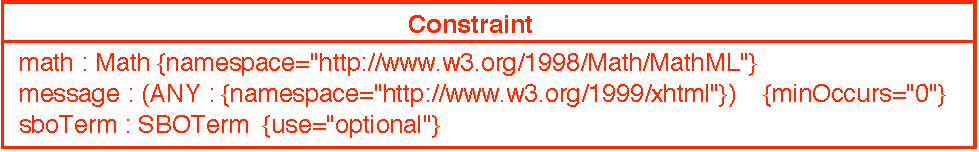
\includegraphics[scale = 0.68]{constraint}
  \vspace*{-1ex}
  \caption{The definition of \class{Constraint}.
    Following UML notation fields
    that are inherited from a base class are not shown.}
  \label{fig:constraint}
  \end{blockChanged}
\end{figure}

A \class{Constraint} structure consists of two fields:
\attrib{math}, which contains a MathML formula, and the optional
field \attrib{message}, which contains a message in XHTML format that may
be displayed to the user.  The formula contained in the
\attrib{math} field should be an arbitrary function of the
variables and parameters of the SBML model.  The formula must
return a boolean value of \texttt{true} when the model is a
\emph{valid} state.  \class{Constraint} structures have effect at
all times, i.e, $t >= 0$.

\class{Constraint} structures \emph{cannot and should not} be used
to compute the dynamical behavior of a model as part of, for
example, simulation. They simply provide a mechanism allowing a
modeler to express the validity of a model's state during
numerical analysis.  Constraints may be used as a key input to
non-dynamical analysis, for example by expressing flux constraints
for flux balance analysis.

The results of a simulation of a model containing a constraint are
invalid from any simulation time at and after a point when the
function given by the \attrib{math} returns a value of
``\attribvalue{false}''. (Invalid simulation results do not make a
prediction of the behavior of the biochemical reaction network
represented by the model.)  The precise behavior of simulation
tools is left undefined with respect to constraints. If invalid
results are detected with respect to a given constraint, the
\attrib{message} field may optionally be displayed to the user.
Software tools are not required to display the message, but it is
recommended as a matter of best practice. The simulation tool may
also halt the simulation or clearly delimit in output data the
simulation time point at which the simulation results become
invalid.

\subsubsection{The \attrib{sboTerm} Field}

The \class{Constraint} structure has an optional \class{SBOTerm}
field, \attrib{sboTerm} (see Section~\ref{sec:sboTerm}).  This
field when present must contain an Systems Biology Ontology
(SBO)\sboref term identifier referring to an actual SBO term.  The
\class{Constraint} structure should have a `is a' relationship
with the SBO term. The SBO term chosen should be the most precise
(narrow) term that matches the form of the \class{Constraint}.

\subsubsection{Example}

As an example, the following SBML fragment demonstrates the
constraint that species $S_1$ should only have values between 1
and 100:

\begin{example}
<listOfConstraints>
    <constraint>
        <math xmlns="http://www.w3.org/1998/Math/MathML">
            <apply>
                <and/>
                <apply>
                    <lt/>
                    <cn> 1 </cn>
                    <ci> S1 </ci>
                </apply>
                <apply>
                    <lt/>
                    <ci> S1 </ci>
                    <cn> 100 </cn>
                </apply>
            </apply>
        </math>
        <message>
            <p xmlns="http://www.w3.org/1999/xhtml">
                Species S1 is out of range
            </p>
        </message>
    </constraint>
</listOfConstraints>
\end{example}

\end{blockChanged}


%-----------------------------------------------------------------------------
\subsection{Reactions}
\label{sec:reactions}
%-----------------------------------------------------------------------------

A \emph{reaction} represents any transformation, transport or binding
process, typically a chemical reaction, that can change the
amount of one or more species.  In SBML, a reaction is defined primarily in
terms of the participating reactants and products (and their corresponding
stoichiometries), along with optional modifier species, an optional kinetic
law describing the rate at which the reaction takes place, and optional
parameters entering into the kinetic law.  These various parts of a
reaction are recorded in the SBML \class{Reaction} type defined in
Figure~\vref{fig:reaction}.

\begin{figure}[htb]
  \vspace*{10pt}
  \centering
  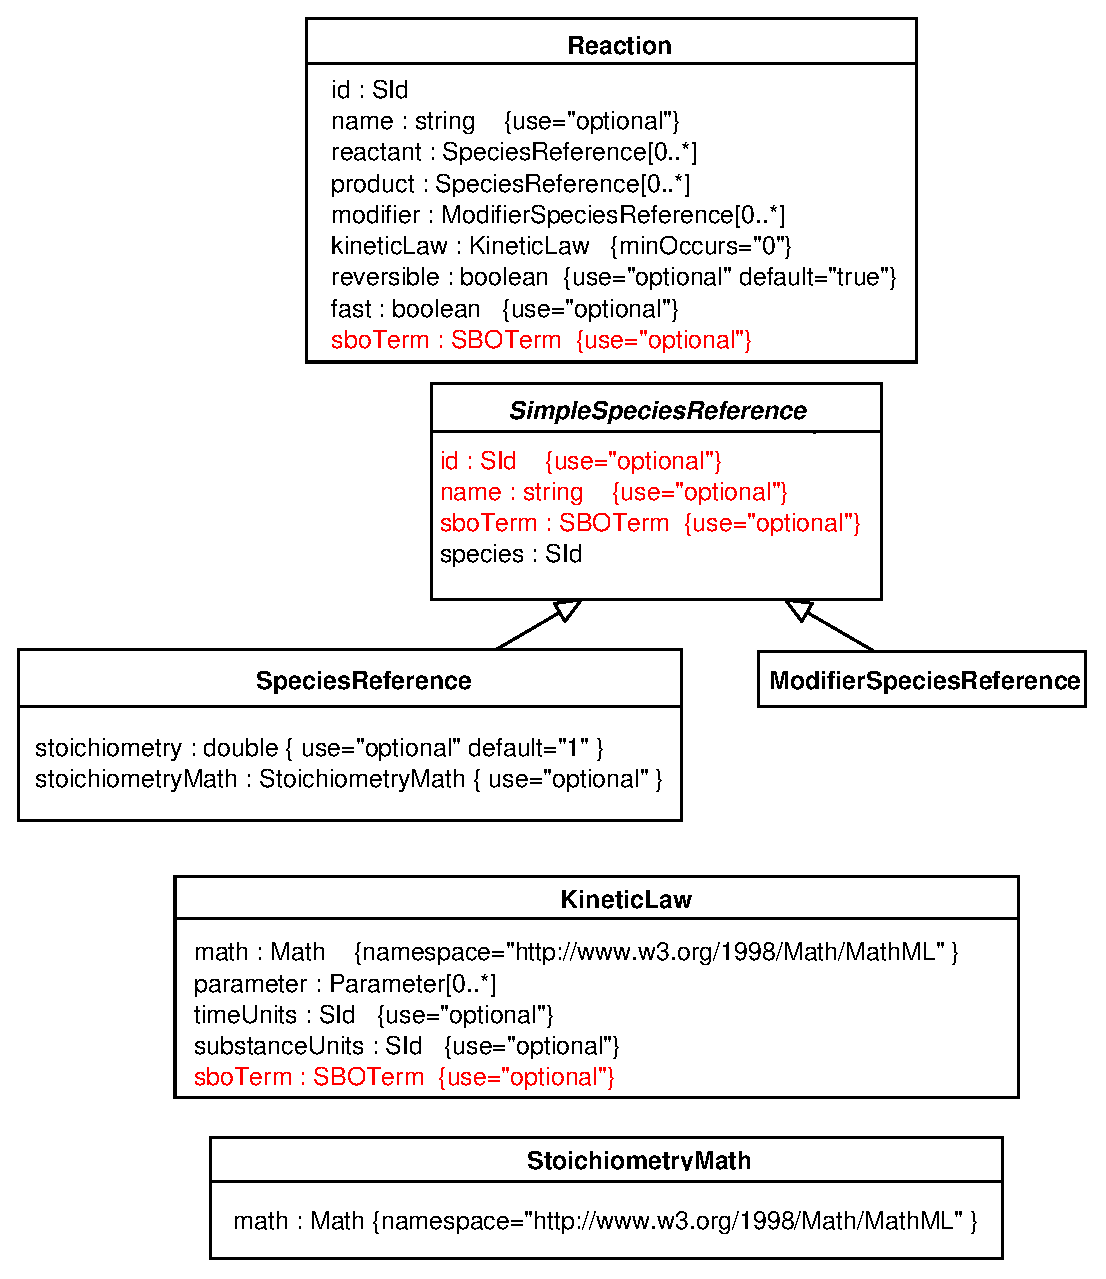
\includegraphics[scale=0.67]{reaction}
  \caption{The definitions of \class{Reaction}, \class{KineticLaw},
    \class{SpeciesReference} and \class{ModiferSpeciesReference}.
    Following UML notation fields
    that are inherited from a base class are not shown.}
  \label{fig:reaction}
\end{figure}


\subsubsection{The \attrib{id} and \attrib{name} Fields}

As with most other main structures in SBML, the \class{Reaction} data
structure includes a required \attrib{id}\changed{, of type \class{SId},} and an optional
\class{name}\changed{, of type \class{string}}.  These must be used according to the guidelines described in
Section~\ref{sec:idnameattribs}.

\begin{blockChanged}
The identifier of a \class{Reaction} structure can be used in mathematical
formulas in an SBML model to represent the rate of the reaction.  This
usage is explained in detail in Section~\ref{subsec:reaction-as-symbol}
below.
\end{blockChanged}


\subsubsection{The \attrib{reactant}, \attrib{product} and \attrib{modifier} Fields}

\begin{blockChanged}
The reactant species, product species and
modifier species in a reaction are described using the fields
\attrib{reactant}, \attrib{product} and \attrib{modifiers}, respectively.
These fields are optional lists of \class{SpeciesReference} and
\class{ModifierSpeciesReference} structures, as shown in
Figure~\vref{fig:reaction}.  They are described in more detail in
Sections~\ref{subsec:speciesreference} and~\ref{subsec:modifierreference}
below.
\end{blockChanged}


\subsubsection{The \attrib{reversible} Field}

The optional boolean field \attrib{reversible} indicates
whether the reaction is reversible.  The field is optional, and if left
unspecified in a model, it defaults to a value of ``\attribvalue{true}''.
Although the reversibility of a reaction is determined by its rate law, the
need to allow rate expressions in SBML to be optional leads to the need for
a \changed{separate} flag indicating reversibility.  Information about reversibility in the
absence of a \attrib{KineticLaw} in a \class{Reaction} is useful in certain
kinds of structural analyses such as elementary mode analysis.  It is true
that the presence of this information in two places (i.e., the rate
expression and the flag \attrib{reversible}) leaves open the possibility of
a model containing contradictory information, but the creation of such a
model would indicate an error on the part of the software generating it.
Software developers must take care to guard against logical contradictions
in the definitions of reactions.


\subsubsection{The \attrib{fast} Field}

The optional boolean field \attrib{fast} is another boolean field in the
\class{Reaction} data structure; a value of ``\attribvalue{true}''
signifies that the given reaction is a ``fast'' one compared to others in
the system being modeled.  This may be relevant when computing equilibrium
concentrations of rapidly equilibrating reactions.  Simulation/analysis
packages may chose to use this information to reduce the number of ODEs
required and thereby optimize such computations.  (A simulator/analysis package
that has no facilities for dealing with fast reactions can ignore this
field. In theory, if the choice of which reactions are fast is
correctly made, then a simulation performed with them should give the same
results as a simulation performed without fast reactions.  However,
currently there appears to be no single unambiguous method for designating
which reactions should be considered fast, and some users may designate a
reaction as fast when in fact it is not.)  The \attrib{fast} field
does not have a default value: a missing value indicates the
modeler does not know or wish to specify the rate of the
reaction relative to other reactions in the model.


\subsubsection{The \attrib{sboTerm} Field}

The \class{Reaction} structure has an optional \class{SBOTerm}
field, \attrib{sboTerm} (see Section~\ref{sec:sboTerm}).  This
field when present must contain an Systems Biology Ontology
(SBO)\sboref term identifier referring to a modeling framework
SBO term, that is a term derived from \sbomodellingframework. The
SBO term chosen should be the most precise (narrow) term that
defines the mathematical framework used in the reaction.


\begin{blockChanged}
\subsubsection{\class{SimpleSpeciesReference}}
\label{subsec:simplespeciesreference}

Every species that enters into a given reaction must appear in
that reaction's lists of reactants, products \changed{and/or} modifiers.  In an
SBML model, all species that \changed{may} participate in any reaction are
listed in the \attrib{listOfSpecies} field of the top-level
\class{Model} data structure (see Section~\ref{sec:model}).  Lists
of products, reactants and modifiers in \class{Reaction}
structures do not introduce new species, but rather, they refer
back to those listed in the model's top-level \attrib{listOfSpecies}.  For
reactants and products, the connection is made using the
\class{SpeciesReference} data structure; for modifiers, it is made
using the \class{ModifierSpeciesReference} data structure.

\class{SimpleSpeciesReference}, defined in Figure~\vref{fig:reaction}, is
an abstract type that serves as the parent class of both
\class{SpeciesReference} and \class{ModifierSpeciesReference}.  It is used
simply to hold the fields \attrib{species}, \attrib{id}, and \attrib{name}
that are common to the latter structures.  The optional identifier stored
in the \attrib{id} field gives the reference an identifier for use in the
reaction's kinetic rate expression (Section~\ref{subsec:kinetic-law}).  The
identifier must be a text string conforming to the syntax permitted by the
\class{SId} data type described in Section~\ref{sec:id}.  The \attrib{id}
value (whether it is in a \class{SpeciesReference} or
\class{ModifierSpeciesReference} object) exists in the global namespace of
the model, as described in Section~\ref{sec:idnameattribs}.
\class{SimpleSpeciesReference} also has an optional \attrib{name} field, of
type \class{string}.  The \attrib{name} and \attrib{id} fields must be used
as described in Section~\ref{sec:idnameattribs}.

\end{blockChanged}


\subsubsection{\class{SpeciesReference}}
\label{subsec:speciesreference}

\begin{blockChanged}
In a given reaction, references to a model's species that act as reactants
and/or products are made using \class{SpeciesReference} data objects.
The mandatory field \attrib{species}, inherited from
\class{SimpleSpeciesReference} (Section~\ref{subsec:simplespeciesreference}),
must refer to the name of an existing species defined in the enclosing
\class{Model} structure.
\end{blockChanged}

\changed{Product and reactant
stoichiometries can be specified using \emph{either} \attrib{stoichiometry} or
\attrib{stoichiometryMath} in the \class{SpeciesReference} structure.}
The \attrib{stoichiometry} field is of type double and should contain values
greater than 0. The \attrib{stoichiometryMath} field is implemented as an
element containing a MathML math expression in dimensionless units.  Only
one of the \attrib{stoichiometry} and \attrib{stoichiometryMath} fields
should be used on a given \class{SpeciesReference} structure.  When neither
field is present then the stoichiometry associated with the
\class{SpeciesReference} structure is ``\attribvalue{1}''.

\changed{For maximum interoperability between models and software tools,
we recommend that when generating SBML Level 2 models,
the \attrib{stoichiometry} field be used} in
preference to the \attrib{stoichiometryMath} field and that the
\attrib{stoichiometry} field contains integer values.  Parsing
software should expect and handle appropriately all possible
values of the \attrib{stoichiometry} and
\attrib{stoichiometryMath} fields including, for example,
non-integer values for \attrib{stoichiometry}. \changed{The
expression in \attrib{stoichiometryMath} may refer to species
identifiers, as discussed in Section~\ref{sec:ci-token}.  The only
species identifiers that can be used in \attrib{stoichiometryMath}
are those listed in the \attrib{reactant}, \attrib{product} and
\attrib{modifier} fields of the containing \class{Reaction}
structure.}

\changed{The \class{SpeciesReference} structure also has an optional
\class{SBOTerm} field, \attrib{sboTerm} (see
Section~\ref{sec:sboTerm}).  When present, this field must contain
a Systems Biology Ontology (SBO)\sboref term identifier referring
to a product or reactant SBO term, that is a term derived from
\sboproduct or \sboreactant respectively.  A product term should
only be used when the \class{SpeciesReference} structure is
contained in the \attrib{product} field of the containing
\class{Reaction} structure.  Similarly a reactant term should only
be used when the \class{SpeciesReference} structure is contained
in the \attrib{reactant} field of the containing \class{Reaction}
structure. The \class{SpeciesReference} structure should have a
`is a' relationship with the SBO term. The SBO term chosen should
be the most precise (narrow) term that captures the role of the
given species in the reaction.}

The following is a simple example of a species reference for species
``X0'', with stoichiometry 2, in a list of reactants within a reaction
named ``J1'':

\begin{example}
<model>
    ...
    <listOfReactions>
        <reaction id="J1">
            <listOfReactants>
                <speciesReference species="X0" stoichiometry="2">
            </listOfReactants>
            ...
        </reaction>
        ...
    </listOfReactions>
    ...
</model>
\end{example}

The following is a more complex example of a species reference for species
``X0'', with a stoichiometry expression consisting of the parameter \texttt{x}:

\begin{example}
<model>
    ...
    <listOfReactions>
        <reaction id="J1">
            <listOfReactants>
                <speciesReference species="X0">
                    <stoichiometryMath>
                        <math xmlns="http://www.w3.org/1998/Math/MathML">
                            <ci>x</ci>
                        </math>
                    </stoichiometryMath>
                </speciesReference>
            </listOfReactants>
            ...
        </reaction>
        ...
    </listOfReactions>
    ...
</model>
\end{example}

A reaction can contain an empty list of reactants or an empty list of
products but must have at least one reactant or product.  Also note that
whether a given species is allowed to appear as a reactant or product is
dictated by certain flags on the structure defining the species in the
model; see Section~\ref{sec:species-constant} for more information.

A species can occur more than once in the lists of reactants and products of a given
reaction.  The effective
stoichiometry for a species in a reaction is the sum of
the stoichiometry values given on the \class{SpeciesReference} structures in the list
of products minus the sum of stoichiometry values given on the
\class{SpeciesReference} structures in the list of reactants.
A positive value indicates the species is effectively a product and a negative
value indicates the species is effectively a reactant.  SBML places no
restrictions on the effective stoichiometry of a species in a reaction; for example,
it can be zero.  In the following SBML fragment, the two reactions have the same
effective stoichiometry for all their species:

\begin{example}
<reaction id="x">
    <listOfReactants>
        <speciesReference species="a"/>
        <speciesReference species="a"/>
        <speciesReference species="b"/>
    </listOfReactants>
    <listOfProducts>
        <speciesReference species="c"/>
        <speciesReference species="b"/>
    </listProducts>
</reaction>
<reaction id="y">
    <listOfReactants>
        <speciesReference species="a" stoichiometry="2"/>
    </listOfReactants>
    <listOfProducts>
        <speciesReference species="c"/>
    </listProducts>
</reaction>
\end{example}

\subsubsection{\class{ModifierSpeciesReference}}
\label{subsec:modifierreference}

\begin{blockChanged}
Sometimes a species appears in the kinetic rate formula of a reaction but
is itself neither created nor destroyed in that reaction (for example,
because it acts as a catalyst or inhibitor).  In SBML, all such species are
simply called \emph{modifiers} without regard to the detailed role of
those species in the model.
The \class{Reaction} structure provides a way to express which
species act as modifiers in a given reaction.  This is the purpose
of the \attrib{modifier} field in \class{Reaction}; this field is
a list of \class{ModifierSpeciesReference} structures defined in
Figure~\vref{fig:reaction}.

The \class{ModifierSpeciesReference} structure has a
mandatory field, \attrib{species}, of type \class{SId}; its value
must be the identifier of a species defined in the enclosing
\class{Model}.   This species is designated as a modifier for the current
reaction.  A reaction may have any number of modifiers.

In common with many other SBML structures, the
\class{ModifierSpeciesReference} structure also has an
optional field named \attrib{id}, used to give the reference an
identifier.  The identifier must be a text string conforming to
the syntax permitted by the \class{SId} data type described in
Section~\ref{sec:id}.  The \attrib{id} value exists in the global
namespace of the model as described in
Section~\ref{sec:idnameattribs}.  \class{ModifierSpeciesReference}
also has an optional \attrib{name} field, of type \class{string}.
The \attrib{name} and \attrib{id} fields \changed{must} be used as
described in Section~\ref{sec:idnameattribs}.

It is permissible for a modifier species to simultaneously appear in the
list of reactants and products of the same reaction where it is
designated as a modifier, as well as to appear in the list of reactants,
products and modifiers of other reactions in the model.

The \class{ModifierSpeciesReference} structure has an optional
\class{SBOTerm} field, \attrib{sboTerm} (see
Section~\ref{sec:sboTerm}).  This field when present must contain
a Systems Biology Ontology (SBO)\sboref term identifier referring
to a modifier SBO term, that is a term derived from \sbomodifier.
The structure containing the \class{sboTerm} field should have a
``is a'' relationship with the SBO term. The SBO term chosen should
be the most precise (narrow) term that captures the role of the
given species in the reaction.

\end{blockChanged}


\subsubsection{\class{KineticLaw}}
\label{subsec:kinetic-law}

A \class{kineticLaw} structure, enclosed in a \class{Reaction} structure,
 describes the rate at which the reaction
takes place.  The inclusion of a \class{KineticLaw} structure in an
instance of a \class{Reaction} component is optional; however, in general
there is no useful default that can be substituted in place of a missing
rate law definition in a reaction.
As shown in Figure~\vref{fig:reaction}, the \class{KineticLaw} structure has a
field called \attrib{math}; this is a MathML expression  defining the
rate of the reaction.

It is important to make clear at the outset that a ``kinetic law'' in SBML
is \emph{not} equivalent to a traditional rate law.  The reason is that
SBML must support multi-compartment models, and the units used in textbook
rate laws as well as some conventional single-compartment modeling packages
are problematic when used for defining reactions between multiple
compartments.  Rate expressions in SBML are expressed in terms of
\quantity{substance}/\quantity{time}, rather than the more typical
\quantity{concentration}/\quantity{time}.  Converting between these two
conventions is a simple matter of dividing the
\quantity{substance}/\quantity{time} expression by the size of the
compartment where a given species is located.  To put this in slightly more
precise terms, suppose there are two species $S$ and $P$ in a reaction
$S \rightarrow P$, where $S$ is located in a compartment $A$ having
volume $V_A$, $P$ is located in a compartment $B$ having volume $V_B$, and
the kinetic law expression gives the rate of the reaction as being $R$.
Then the rate of change in the concentration of $S$ is given by $d[S]_A/dt
= -R/V_A$ and the rate of change in the concentration of $P$ is $d[P]_B/dt
= R/V_B$.  The translation of a complete multi-compartmental model into
ODEs is given in Section~\ref{sec:odeeg}.

\changed{The expression in \attrib{math} may refer to species
identifiers, as discussed in Section~\ref{sec:ci-token}.}  The
only species identifiers that can be used in \attrib{math} are
those listed in the \attrib{reactant}, \attrib{product} and
\attrib{modifier} fields of the \class{Reaction} structure.

As previously stated, the overall rate expression in the
\attrib{math} field must have the units of
\quantity{substance/time}.  The optional fields
\attrib{substanceUnits} and \attrib{timeUnits} determine the units
of substance and time for the reaction, respectively. The values of
these fields must be chosen from one of the following
possibilities: one of the base unit names from
Table~\vref{tab:unitkind}; one of the built-in unit names
appearing in the first column of Table~\vref{tab:builtin}); or the
name of a new unit defined in the list of unit definitions in the
enclosing \class{Model} structure.  \changed{In the case of
\attrib{substanceUnits}, the value chosen must be a scaled and/or
multiplied variant of \unit{dimensionless}, \unit{moles}, \unit{kilogram} or
\unit{item}. In the case of \attrib{timeUnits}, the value chosen
must be a scaled and/or multiplied variant of \unit{seconds} or
\unit{dimensionless}}. If these fields are not set in a given
\class{KineticLaw} instance, the units are taken from the defaults
defined by the built-in ``\unit{substance}'' and ``\unit{time}''
of Table~\vref{tab:builtin}.

An instance of a \class{KineticLaw} type structure can contain zero or more
\class{parameter} structures (Section~\ref{sec:parameters}) which define
symbols that can be used in the \attrib{math} field.  As discussed in
Section~\ref{sec:namespaces}, reactions introduce local namespaces for
parameter identifiers.  Within a \class{KineticLaw} structure inside a
reaction definition, a local parameter whose identifier is identical to a
global parameter defined in the enclosing \class{Model}-type structure
takes precedence over that global parameter.

\begin{blockChanged}
The \class{KineticLaw} structure has an optional \class{SBOTerm}
field, \attrib{sboTerm} (see Section~\ref{sec:sboTerm}).  This
field when present must contain a Systems Biology Ontology
(SBO)\sboref term identifier referring to a kinetic law SBO term,
that is a term derived from \sbokineticlaw.  The
\class{KineticLaw} structure should have a `is a' relationship
with the SBO term. The SBO term chosen should be the most precise
(narrow) term that defines the type of kinetic law encoded by the
structure.

The following is an example of a \class{Reaction} structure that
defines a reaction named $J_1$, in which $X_0 \rightarrow S_1$ at
a rate given by $k X_0 S_2$, in conventional units, where $S_2$ is
a catalyst and $k$ is a parameter.  It demonstrates the use of
species references and the \class{KineticLaw} structure.  The
units on the species here are the defaults of
\quantity{substance}/\quantity{volume} (see
Section~\ref{sec:species}), and so the conventional rate
expression is multiplied by the compartment volume so that the
encoded rate expression has the final units of
\quantity{substance/time}.

\begin{example}

<model>
    ...
    <listOfUnitDefinitions>
        <unitDefinition id="concent_per_time">
            <listOfUnits>
                <unit kind="litre"/>
                <unit kind="mole"   exponent="-1"/>
                <unit kind="second" exponent="-1"/>
            </listOfUnits>
        </unitDefinition>
    </listOfUnitDefinitions>
    ...
    <listOfSpecies>
        <species id="S1" compartment="c1" initialConcentration="2.0"/>
        <species id="S2" compartment="c1" initialConcentration="0.5"/>
        <species id="X0" compartment="c1" initialConcentration="1.0"/>
    </listOfSpecies>
        ...
    <listOfReactions>
        <reaction id="J1">
            <listOfReactants>
                <speciesReference species="X0"/>
            </listOfReactants>
            <listOfProducts>
                <speciesReference species="S1"/>
            </listOfProducts>
            <listOfModifiers>
                <modifierSpeciesReference species="S2"/>
            </listOfModifiers>
            <kineticLaw>
                <math xmlns="http://www.w3.org/1998/Math/MathML">
                    <apply>
                        <times/>
                        <ci> k </ci>
                        <ci> S2 </ci>
                        <ci> X0 </ci>
                        <ci> c1 </ci>
                    </apply>
                </math>
                <listOfParameters>
                    <parameter id="k" value="0.1" units="concent_per_time"/>
                </listOfParameters>
            </kineticLaw>
        </reaction>
    </listOfReactions>
    ...
</model>
\end{example}
\end{blockChanged}


\begin{blockChanged}
\subsubsection{Reaction Identifiers Used in Mathematical Expressions}
\label{subsec:reaction-as-symbol}

The value of the \attrib{id} field of a \class{Reaction} structure
can be used as the content of a MathML \class{ci} element. Such a
\class{ci} element or symbol represents the rate of the given
reaction as given by the \class{KineticLaw} structure of the
reaction.  The symbol has the units of the \class{KineticLaw} as
described in Section~\ref{subsec:kinetic-law} or
\quantity{substance/time} units if the \class{KineticLaw} is not
present.

A \class{KineticLaw} structure forms an assignment statement
assigning the evaluated value of the \attrib{math} field to the
symbol value contained in the \class{Reaction} \attrib{id} field.
No other structure can assign a value to such a reaction symbol;
i.e., the \attrib{variable} fields of \class{InitialAssignment},
\class{RateRule}, \class{AssignmentRule} and
\class{EventAssignment} structures cannot contain the value of a
\class{Reaction} \attrib{id} field.

The combined set of \class{InitialAssignment},
\class{AssignmentRule} and \class{KineticLaw} structures form a
set of assignment statement that should be considered as a whole.
The combined set of assignment rules should not contain algebraic
loops: a chain of dependency between these statements should
terminate.  (More formally, consider the directed graph of assignment
statements where nodes are statements and directed arcs exist for
each occurrence of a symbol in a assignment statement
\attrib{math} field. The directed arcs start from the statement
defining the symbol to the statements that contain the symbol in
their math fields. Such a graph must be acyclic.)  Examples of valid
and invalid set of assignment statements are given in
Section~\ref{sec:ruleconstraints}.

\end{blockChanged}

%-----------------------------------------------------------------------------
\subsection{Events}
\label{sec:events}
%-----------------------------------------------------------------------------

\class{Model} has an optional list of \class{Event} structures that
describe the time and form of explicit instantaneous discontinuous state
changes in the model.  For example, an event may describe that one species
concentration is halved when another species concentration exceeds a given
threshold value.

An \class{Event} structure defines when the event can occur, the variables
that are affected by the event, and how the variables are affected.  The
effect of the event can optionally be delayed after the occurrence of the
condition which invokes it.  The operation of an \class{Event} structure is
divided into two phases (even when the event is not delayed): one when the
event is \emph{fired} and the other when the event is \emph{executed}. The
\class{Event} type is defined in Figure~\vref{fig:event}.  Both
\class{Event} and \class{EventAssignment} are derived from \class{SBase}
(see Section~\ref{sec:sbase}).  An example of a model which uses events is
given below.

\begin{figure}[htb]
  \centering
  
\includegraphics[scale = 0.68]{event}
  \caption{The definitions of \class{Event} and \class{EventAssignment}.
    Following UML notation, additional fields
    that are inherited from a base class, in this case \class{SBase}, are not shown.}
  \label{fig:event}
\end{figure}

\subsubsection{The \attrib{id} and \attrib{name} Fields}
These optional fields are available to support external references
to event structures.  These fields operate in the manner described in
Section~\ref{sec:idnameattribs} except that the \attrib{id} field is optional.

\subsubsection{The \attrib{trigger} Field}
The \attrib{trigger} field defines when the \class{Event} structure has an
effect on the model.  The \attrib{trigger} field contains a MathML boolean
expression.  The exact instant that the expression evaluates to true is the
time point when the \class{Event} is \emph{fired}.  The event only fires
when the \attrib{trigger} makes the transition from false to true.  The
event will fire at any further time points when the \attrib{trigger} make
this transition.

\subsubsection{The \attrib{delay} Field}
The optional \attrib{delay} field defines the length of time after
the event has \emph{fired} that the event is \emph{executed}. The
\attrib{delay} field is another MathML expression.  This
expression should be evaluated when the rule is \emph{fired}.  The
default value for the \attrib{delay} field is 0.  The value of the
\attrib{delay} field should always be positive.  The units of the \attrib{delay}
field are those given on the \attrib{timeUnits} field.

\subsubsection{The \attrib{timeUnits} Field}
\label{sec:event-timeunits}

The optional field \attrib{timeUnits} determines the units of time
that apply to the \attrib{delay} field.
The value of the \attrib{timeUnits} field must be either
``\unit{second}'' or ``\unit{dimensionless}'' from Table~\vref{tab:unitkind}, ``\unit{time}'' from
Table~\vref{tab:builtin},
or a new unit defined by a unit definition in the enclosing model
which must be a variant of ``\unit{second}'' units.
The default value of the \attrib{timeUnits} field is
``\unit{time}''.

\subsubsection{The \attrib{eventAssignment} Field}
\label{sec:eventassignment}

The \attrib{eventAssignment} field consists of a non-empty list of
\class{EventAssignment} structures.  This field is implemented as
a \class{listOfEventAssignments} element containing one or more
\class{eventAssignment} elements.  The \class{EventAssignment}
structures represent variable assignments that have effect when
the event is \emph{executed}. The \class{Assignment} structure is
shown in Figure~\ref{fig:event}. The \attrib{variable} field is of
type \class{SId} and contains the identifier of a variable i.e. a
compartment, species or parameter.  \changed{The \attrib{variable}
field must not contain the identifier of a reaction.  The values
of the \attrib{variable} field must be unique among the set of
\class{EventAssignment} structures within an \class{Event}
structure.} The structures referenced by the \attrib{variable}
field must have their \attrib{constant} fields set to
``\attribvalue{false}''. The \attrib{math} field contains a MathML
expression that defines the new value of the variable. This
expression is evaluated when the \class{Event} is \emph{fired} but
the variable only acquires the result or new value when the
\class{Event} is \emph{executed}. The order of the
\class{EventAssignment} structures is not significant; the effect
of one assignment cannot affect the result of another assignment.
The identifiers occurring in the MathML \attrib{ci} fields of the
\class{EventAssignment} structures represent the value of the
identifier at the point when the \class{Event} is \emph{fired}.

\changed{A variable cannot be assigned a value in an
\class{EventAssignment} structure and be assigned a value by an
\class{AssignmentRule} structure i.e. the value of a
\attrib{variable} attribute on a \class{EventAssignment} structure
cannot be the same as the value of a \attrib{variable} attribute
on a \class{AssignmentRule} structure.  This restriction is
imposed because in the invalid case the EventAssignment is
redundant because the variable would assume the value of given by
the \class{AssignmentRule}.}

In all cases, as would be expected, the units of the formula
\changed{ in a \class{EventAssignment}} are identical to the units
associated with the \attrib{variable} field, when that variable
appears in other formulas. However, the precise details, which are
identical to those of \class{AssignmentRule} structures, depend on
the variable that is being set:

\begin{itemize}

\item \emph{In the case of a species}, an \class{EventAssignment} sets the
  referenced species' quantity (\quantity{concentration} or
  \quantity{amount of substance})
  to the value determined by the formula
  in \attrib{math}.  The units of the formula are the \emph{units of the species} as
  defined in Section~\ref{sec:species-units}.

\item \emph{In the case of a compartment}, an \class{EventAssignment} sets
  the referenced compartment's size to the size determined by the formula
  in \attrib{math}.  The overall units of the formula are the units
  specified for the size of the compartment identified by the value of the
  \class{EventAssignment}'s \attrib{variable} field.  (See
  Section~\ref{sec:compartment-units} for an explanation of how the units of the
  compartment's size are determined.)

\item \emph{In the case of a parameter}, an \class{EventAssignment} sets the
  referenced parameter's value to that determined by the formula in
  \attrib{math}.  The overall units of the formula are the units
  defined for the parameter identified by the value of the
  \class{EventAssignment}'s \attrib{variable} field.  (See
  Section~\ref{sec:parameter-units} for an explanation of how the units of the
  parameter are determined.)

\end{itemize}

\subsubsection{Example \class{Event} structure}

A example of an \class{Event} structure follows.  This structure makes the
assignment $k_2 = 0$ at the point when $P_1 \leq t$:

\begin{example}
<event>
    <trigger>
        <math xmlns="http://www.w3.org/1998/Math/MathML">
            <apply>
                <leq/>
                <ci> P1 </ci>
                <ci> t </ci>
            </apply>
        </math>
    </trigger>
    <listOfEventAssignments>
        <eventAssignment variable="k2">
            <math xmlns="http://www.w3.org/1998/Math/MathML">
                <cn> 0 </cn>
            </math>
        </eventAssignment>
    <listOfEventAssignments>
</event>
\end{example}

A complete example of a model using events is given in Section~\ref{sec:eventeg}.

\subsubsection{Detailed semantics of events}

The description of events above describes the action of events in isolation from
each other.  This section describes how events interact.  Events whose \attrib{trigger}
expression is true at the start of a simulation do not \emph{fire} at the start of the simulation.
Events \emph{fire} only when the trigger \emph{becomes} true, i.e. the trigger expression
transitions from false to true.  It is possible for events to \emph{fire} other events, i.e. an
event assignment can cause an event to \emph{fire}, therefore it is possible for model to be entirely
encoded in \class{Event} structures.

\changed{\emph{Any} transition of a \attrib{trigger} expression
from false to true will cause an \class{event} to \emph{fire}.
Consider an \class{event} $E$ with delay $d$ where the
\attrib{trigger} expression makes a transition from false to true
at times $t_1$ and $t_2$.  The \class{EventAssignment} structure
will have effect at $t_1+d$ and $t_2+d$ irrespective of the
relative times of $t_1$ and $t_2$. For example events can
``overlap'' so that $t_1 < t_2 < t_1+d$ still causes an event
assignments to occur at $t_1+d$ and $t_2+d$.}

It is entirely possible for two events to be \emph{executed} simultaneously in simulated time.
It is assumed that, although the precise time at which these events are \emph{executed} is not
resolved beyond the given point in simulated time, the order in which the events occur is resolved.
This order can be significant in determining the overall outcome of a given simulation. SBML Level
2 does not define the algorithm for determining this order (the tie-breaking algorithm).  As a
result, the results of simulations involving events may vary when simultaneous events occur during
simulation.  It is anticipated that future versions or levels of SBML will define a specific set
of tie-breaking algorithms and a mechanism for models to indicate which algorithm should be
applied during simulation.

Despite the absence of a specific tie-breaking algorithm, SBML event simulation is constrained as
follows. When an event $X$ \emph{fires} another event $Y$ and event $Y$ has zero delay then event
$Y$ is added to the existing set of simultaneous events that are pending \emph{execution}. Events
such as $Y$ do not have a special priority or ordering within the tie-breaking algorithm. Events
$X$ and $Y$ form a cascade of events at the same point in simulation time.  All events in a model
are open to being in a cascade.  The position of an event in the event list does not affect whether
it can be in the cascade: $Y$ can be triggered whether it is before or after $X$ in the list of
events.  A cascade of events can be infinite (never terminate).  When this occurs a simulator
should indicate this has occurred, i.e. it is incorrect for the simulator to arbitrarily break the
cascade and continue the simulation without at least indicating the infinite cascade occurred.
A variable can change more than once when processing simultaneous events at simulation
time $t$.  The model behavior (output) for such a variable is the value of the
variable at the end of processing all the simultaneous events at time $t$.

\changed{It is not possible for an event to be triggered when
simulation time is zero ($t=0$).  All variables are nominally
assumed to have their initial conditions at any time before $t=0$
(to do otherwise assumes simulation before $t=0$).  The time
symbol can never have a negative value.  As result no transition
in variable values or expressions can occur at $t=0$ and thus no
events can be triggered at that point in simulation time.}


\begin{blockChanged}
%=============================================================================
\section{A standard Format for the \attrib{annotation} Field}
\label{sec:finney-novere}
%=============================================================================

This section describes the standard non-proprietary format for
\class{annotation} elements when (a) referring to controlled
vocabulary terms and database identifiers which define and
describe biological and biochemical entities; and (b) describing
the creator of a model and its modification history. This format
uses a restricted form of Dublin Core~\citep{DCMI:2003} elements
embedded in RDF~\citep{w3c:2004}.

This format should not be used to refer to Systems Biology
Ontology (SBO)\sboref terms because SBO defines terms about
mathematical modelling constructs and not the biological and
biochemical entities that the mathematics represent.

The format uses a number of external XML standards and associated
XML namespaces. Table~\ref{tab:namespaces-for-standard-annotation}
lists these namespaces and relevant documentation on those
namespaces.  The format described here constrains the order of
elements in these namespaces beyond the constraints defined in the
standard definitions for those namespaces.  For each standard
listed the format only uses a subset of the possible syntax
defined by the given standard.  Thus it is possible for an
\class{annotation} element to include XML that is compliant with
those external standards but is not compliant with the format
described here.  Parsers wishing to support this format should be
aware that a valid \class{annotation} element may contain an
\class{rdf:RDF} element which is not compliant with the format
described here.  A parser should check that all aspects of the
syntax defined here before assuming that the contained data is
encoded in the format.

\begin{table}[bh]
  \begin{blockChanged}
  \small
  \centering
  \begin{tabular}{lll}
    \toprule
    Namespace Prefix & Namespace URI & Definition Document \\
    \midrule
    \class{dc} & \url{http://purl.org/dc/elements/1.1/} & \citep{powell:2003}\\
    \class{rdf} & \url{http://www.w3.org/1999/02/22-rdf-syntax-ns\#} & \citep{w3c:2004b} \\
    \class{dcterms} & \url{http://purl.org/dc/terms/} & \citep{kokkelink:2002}\\
    & & \citep{DCMIUB:2005} \\
    \class{vcard} & \url{http://www.w3.org/2001/vcard-rdf/3.0#"} & \citep{iannella:2001} \\
    \bottomrule
  \end{tabular}
  \vspace*{-0.95ex}
  \caption{The XML standards used in the SBML standard format for annotation.
  The namespace prefix are shown to indicate only the prefix used in the main text.}
  \label{tab:namespaces-for-standard-annotation}
  \end{blockChanged}
\end{table}

%=============================================================================
\subsection{General Syntax for Dubin Core annotation}
%=============================================================================

An outline of the format syntax is shown below.

\begin{example}
<SBML_ELEMENT +++ metaid="SBML_META_ID" +++ >
  +++
  <annotation>
    +++
    <rdf:RDF
      xmlns:rdf="http://www.w3.org/1999/02/22-rdf-syntax-ns\#"
      xmlns:dc="http://purl.org/dc/elements/1.1/"
      xmlns:dcterm="http://purl.org/dc/terms/"
    >
      <rdf:Description rdf:about="#SBML_META_ID">
        [MODEL_HISTORY]
        <DUBLIN_CORE_RELATION_ELEMENT>
          <rdf:Bag>
            <rdf:li rdf:resource="URI" />
            ...
          </rdf:Bag>
        </DUBLIN_CORE_RELATION_ELEMENT>
        ...
      </rdf:Description>
      +++
    </rdf:RDF>
    +++
  </annotation>
  +++
</SBML_ELEMENT>
\end{example}

In the above outline shows the order of the elements. The
capitalized identifiers refer to generic strings of a particular
type: \texttt{SBML\_ELEMENT} refers to any SBML element name that
can contain an \class{annotation} element; \texttt{SBML\_META\_ID}
is a XML \class{ID} string;
\texttt{DUBLIN\_CORE\_RELATION\_ELEMENT} refers to a restricted
subset of element names in the
\url{http://purl.org/dc/elements/1.1/} and
\url{http://purl.org/dc/terms/} namespaces; and \texttt{URI} is a
URI.  \texttt{[MODEL\_HISTORY]} refers to an optional section
described in Section~\ref{sec:model-history-annotation} which can
only be present within SBML model elements. `\texttt{+++}' is a
placeholder for either no content or valid XML syntax that is not
defined by the standard annotation scheme but is consistent with
the relevant standards for the enclosing elements. `\texttt{...}'
is a placeholder for zero or more elements of the same form as the
immediately preceding element.  The precise form of whitespace and
the XML namespace prefix definitions is not constrained.  The rest
of this section describes the format formally in English.

In this format the annotation of an element is located in a single
\class{rdf:RDF} element contained within an SBML
\class{annotation} element. The annotation element can contain
other elements in any order as described in Section \emph{FIX ME}.
The format described in this section only defines the form of the
\class{rdf:RDF} element. The containing SBML \class{SBase} element
must have a \attrib{metaid} field value. (As this attribute is of
the type \class{ID} its value must unique to the entire SBML
document.)

The first element of the \class{rdf:RDF} element must be an
\class{rdf:Description} element with an \attrib{rdf:about}
attribute. (This format doesn't define the form of subsequent
elements of the \class{rdf:RDF} element.) The value of the
\attrib{rdf:about} attribute must be of the form
\texttt{\#<string>} where the string component is equal to the
value of the \attrib{metaid} field of the containing SBML element.

The \class{rdf:Description} element must contain only an optional
model history section (see
Section~\ref{sec:model-history-annotation} followed by a sequence
of zero or more Dublin Core relation elements. The optional model
history section can only be present within an SBML \class{model}
element. The specific type of the relation elements will vary
depending on the relationship between the SBML component and
referenced information or resource.

Whilst Section~\ref{sec:qualified-dc-annotation} describes the
detailed semantics of each of the relation element types the
content of these elements follows exactly the same form.  The
Dublin Core relation elements must only contain a single
\class{rdf:Bag} element which in turn must only contain one or
more \class{rdf:li} elements.  The \class{rdf:li} elements must
only have a \attrib{rdf:resource} attribute containing a URI
referring to an information resource (See
Section~\ref{sec:uri-in-annotation}).

Annotations in this format can be located at different depths
within a model component as is appropriate.

%=============================================================================
\subsection{Use of URIs}
\label{sec:uri-in-annotation}
%=============================================================================

The format represents a set of relationships between the SBML
element and the resources referred to by the contained
\attrib{rdf:resource} attribute values.  The Dublin core relation
elements simply define the type of the relationship.

For instance a \class{Species} element representing a protein
could be annotated with a reference to the database UniProt by the
\url{http://www.uniprot.org/\#P12999} resource identifier,
identifying exactly the protein described by the \class{Species}
element. This identifier maps to a unique entry in UniProt which
is never deleted from the database. In the case of UniProt, this
is the ``accession'' of the entry. When the entry is merged with
another one, both ``accession'' are conserved. Similarly in a
controlled vocabulary resource, each term is associated with a
perenial identifier. The UniProt entry also possess an ``entry
name'' (the Swiss-Prot ``identifier''), a ``protein name'',
``synonyms'' etc. Only the ``accession'' is perennial and should
be used.

The value of the \texttt{rdf:resource} attribute is a URI that
both uniquely identifies the resource, and the data in the
resource. In this case the resource constraining the identifier
precedes the '\#' symbol and the term or database identifier
follows the '\#' symbol. In the present example, the resource
\url{http://www.uniprot.org/} includes the entry P12999.

The value of the \texttt{rdf:resource} attribute is a URI, not a
URL; as such, a URI does not have to reference a physical web
object but just identifies a controlled vocabulary term or
database object (think of a URI as a label that, in this case,
just happens to look like a URL). For instance, the URL
\url{http://www.uniprot.org/entry/P12999} would correspond to the
URI \url{http://www.uniprot.org/\#P12999}.

SBML does not specify how a parser is to interpret a URI. In the
case of a transformation into a physical URL, there could be
several solutions. For instance, the URI
\url{http://www.geneontology.org/\#GO:0007268} can be translated
into:

\noindent \url{http://www.ebi.ac.uk/ego/DisplayGoTerm?selected=GO:0007268}\\
\noindent \url{http://www.godatabase.org/cgi-bin/amigo/go.cgi?view=details\&query=GO:0007268}\\
\noindent
\url{http://www.informatics.jax.org/searches/GO.cgi?id=GO:0007268}

Similarly the URI \url{http://www.ebi.ac.uk/intenz/\#EC 3.5.4.4}
can refer to:

\noindent \url{http://www.ebi.ac.uk/intenz/query?cmd=SearchEC\&ec=3.5.4.4}\\
\noindent \url{http://www.expasy.org/cgi-bin/nicezyme.pl?3.5.4.4}\\
\noindent \url{http://www.chem.qmul.ac.uk/iubmb/enzyme/EC3/5/4/4.html}\\
\noindent \url{http://www.genome.jp/dbget-bin/www_bget?ec:3.5.4.4}\\
\noindent etc.

To enable interoperability, the community has agreed on an initial
set of standardized valid URI syntax rules which may be used
within the standard annotation format. This set of rules is not
part of the SBML standard but will grow independently from
specific SBML Levels and Versions. As the set changes a given URI
syntax rule will not be modified although the physical resource
associated with the rule may change. These URIs will always be
composed as \texttt{resource\#id}. The web page \url{FIX ME} lists
URI syntaxes and possible physical links to controlled vocabulary
and databases. Each entry contains a list of SBML and relation
elements in which the given URI can be appropriately embedded. To
enable consistent and thus useful links to external resources the
URI syntax rule set must have a consistent view of the concepts
represented by the different SBML elements for the purposes of
this format.  For example as the rule set is designed to link SBML
biological and biochemical resources the rule set assumes that a
\class{species} element represents the concept of a biochemical
entity type rather than mathematical symbol. The URI rule list
will evolve with the evolution of databases and resources. The
annotation format described in this section does not require
software to access this list to operate.

%=============================================================================
\subsection{Relation Elements}
\label{sec:qualified-dc-annotation}
%=============================================================================

To enable the format to encode different types of relationships
between SBML elements and resources different Dublin Core elements
are used to enclose a set of \class{rdf:li} elements.  These
elements are either \class{dc:element}\citep{beckett:2002} or a
subset of \class{dcterms:*} elements~\citep{kokkelink:2002}. The
valid set of \class{dcterms:*} elements consists of
\class{dcterms:hasPart}, \class{dcterms:isPartOf},
\class{dcterms:isVersionOf}, \class{dcterms:hasVersion} and
\class{dcterms:isReferencedBy}. The broad semantics of these
elements is defined by the qualified Dublin Core.  The format
adopts a semantics for \class{dc:relation} that is significantly
more constrained than that defined by the Dublin Core standard:
\class{dc:relation} represents the case where the object
represented by the SBML component \emph{is} the subject of the
referenced resource.

The detailed semantics (i.e. from the perspective of automatic
parser) of the relation elements depend on the consistent view of
the concepts represented by the SBML element that is defined by
the URI list at \url{FIX ME} and thus is outside the scope of
SBML.  The URI list generally assumes that the biological entity
represented by the element is the concept linked to the reference
resource.

%\begin{figure}[htb]
%  \vspace*{2pt}
%  \centering
%\[
%%\begin{CD}
%\textrm{SBML Element}  @>{qualifier}>> \textrm{Referenced Resource} \\
%@VV{represents}V                @VV{represents}V \\
%\textrm{Biological Entity A}   @>{relationship}>>
%\textrm{Biological Entity B}
%%\end{CD}
%\]
%  \caption{How the relationship between biological
%  entities are defined using relations between resources}
%  \label{fig:lenovere-annotation}
%\end{figure}

As a guide to maximal interoperability the following is a list of
the semantics of the relation elements, derived from the Dublin
Core standard, interpreted in the context of URIs taken from the
URI list.

\begin{itemize}
\item \class{dc:relation} The object represented by the SBML
component is the subject of the referenced resource

\item \class{dcterms:hasPart} The object represented by the SBML
component includes the subject of the referenced resource, either
physically or logically

\item \class{dcterms:isPartOf} The object represented by the SBML
component is a physical or logical part of the subject of the
referenced resource

\item \class{dcterms:isVersionOf} The object represented by the
SBML component is a version or an instance of the subject of the
referenced resource

\item \class{dcterms:hasVersion} The subject of the referenced
resource is a version or an instance of the object represented by
the SBML component

\item \class{dcterms:isReferencedBy} The object represented by the
SBML component is pointed to by the referenced resource.  This
relation should be used to link SBML components to literature that
describes the component.
\end{itemize}

%===============================================================
\subsection{Model History}
\label{sec:model-history-annotation}
%================================================================

The described format, when enclosed in an SBML \class{model}
element, can include additional elements to describe the history
of the model.  This history data must occur immediately before the
first Dublin Core relation elements.  These additional elements
encode information on the model creator and a sequence of dates
recording changes to the model. The syntax for this section is
outlined below.

\begin{example}
<dc:creator rdf:parseType="Resource">
  <rdf:Bag>
    <rdf:li rdf:parseType="Resource">
      [[
      +++
      <vCard:N rdf:parseType="Resource">
        <vCard:Family>FAMILY_NAME</vCard:Family>
        <vCard:Given>GIVEN_NAME</vCard:Given>
      </vCard:N>
      +++
      [<vCard:EMAIL>EMAIL_ADDRESS</vCard:EMAIL>]
      +++
      [<vCard:ORG>
        <vCard:Orgname>ORGANIZATION_NAME</vCard:Orgname>
      </vCard:ORG>]
      +++
      ]]
    </rdf:li>
    ...
  </rdf:Bag>
</dc:creator>
<dcterms:created rdf:parseType="Resource">
  <dcterms:W3CDTF>DATE<dcterms:W3CDTF>
</dcterms:created>
{<dcterms:modified rdf:parseType="Resource">
  <dcterms:W3CDTF>DATE<dcterms:W3CDTF>
</dcterms:modified>}
\end{example}

The order of elements is as shown above except that elements of
the format contained between \texttt{[[} and \texttt{]]} can occur
in any order.  The capitalized identifiers refer to generic
strings of a particular type: \texttt{FAMILY\_NAME} is the family
name of a person who created the model; \texttt{GIVEN\_NAME} is
the family name of the same person who created the model;
\texttt{EMAIL\_ADDRESS} is the email address of the same person
who created the model; and \texttt{ORGANIZATION\_NAME} is the name
of the organization with which the same person who created the
model is affiliated \texttt{DATE} is a date in W3C date
format~\citep{wolf:1998}. \texttt{W3CDTF}, \texttt{N},
\texttt{ORG} and \texttt{EMAIL} are literal strings. The elements
of the format contained between \texttt{[} and \texttt{]} are
optional. `\texttt{+++}' is a placeholder for either no content or
valid XML syntax that is not defined by the standard annotation
scheme but is consistent with the relevant standards for the
enclosing elements. `\texttt{...}' is a placeholder for zero or
more elements of the same form as the immediately preceding
element. The precise form of whitespace and the XML namespace
prefix definitions is not constrained.  The remaining text in this
section describes the syntax formally in English.

The additional elements of the model history sub-format consist in
sequence of a \class{dc:creator} element, a
\class{dcterms:created} element and zero or more
\class{dcterms:modified} elements.  All these elements must have
the attribute \attrib{rdf:parseType} set to \texttt{Resource}.

The \class{dc:creator} element describes the person who created
the SBML encoding of the model and contains a single
\class{rdf:Bag} element.  The \class{rdf:Bag} element can contain
any number of elements however the first element must be a
\class{rdf:li} element.  The  \class{rdf:li} element can contain
any number of elements in any order.  The set of elements
contained with the \class{rdf:li} element can include the
following informative elements: \class{vCard:N},
\class{vCard:EMAIL} and \class{vCard:ORG}.  The \class{vCard:N}
contains the name of the creator and must consist of a sequence of
two elements: \class{vCard:Family} and the \class{vCard:Given}
whose content is the family (surname) and given (first) names of
the creator respectively.  The \class{vCard:N} must have the
attribute \attrib{rdf:parseType} set to \texttt{Resource}.  The
content of the \class{vCard:EMAIL} element must be the email
address of the creator.  The content of the \class{vCard:ORG}
element must contain a single \class{vCard:Orgname} element.  The
\class{vCard:Orgname} element must contain the name of an
organization to which the creator is affiliated.

The \class{dcterms:created} and \class{dcterms:modified} elements
must each contain a single \class{dcterms:W3CDTF} element whose
content is a date in W3C date format~\citep{wolf:1998} which is a
a profile of (restricted form of) ISO 8601.

%================================================================
\subsection{Examples}
%=================================================================

The following example shows a \class{Reaction} structure annotated
with a reference to a GO term that precisely defines the function
of the reaction.

\begin{example}
<reaction id="calciumBinding" metaid="jb007">
  <annotation>
    <rdf:RDF
      xmlns:dc="http://purl.org/dc/elements/1.1/"
      xmlns:dcterms="http://purl.org/dc/terms/"
      xmlns:rdf="http://www.w3.org/1999/02/22-rdf-syntax-ns\#"
    >
      <rdf:Description rdf:about="#jb007">
        <dc:relation>
          <rdf:Bag>
            <rdf:li rdf:resource="http://www.geneontology.org/\#GO:0005509"/>
          </rdf:Bag>
        </dc:relation>
      </rdf:Description>
    </rdf:RDF>
  </annotation>
  <listOfReactants>
    <speciesReference species="calmodulin"/>
    <speciesReference species="calcium" stoichiometry="4"/>
  </listOfReactants>
  <listOfProducts>
    <speciesReference species="calcium_calmodulin"/>
  </listOfProducts>
</reaction>
\end{example}

The following example describes a species that represents a
complex between the protein calmodulin and calcium ions:

\begin{example}
<species id="Ca_calmodulin" metaid="cacam">
  <annotation>
    <rdf:RDF
      xmlns:rdf="http://www.w3.org/1999/02/22-rdf-syntax-ns\#"
      xmlns:dc="http://purl.org/dc/elements/1.1/"
      xmlns:dcterms="http://purl.org/dc/terms/"
    >
      <rdf:Description rdf:about="\#cacam">
        <dcterms:hasPart>
          <rdf:Bag>
            <rdf:li rdf:resource="http://www.uniprot.org/\#P62158"/>
            <rdf:li rdf:resource="http://www.genome.jp/kegg/compound/\#C00076"/>
          </rdf:Bag>
        </dcterms:hasPart>
      </rdf:Description>
    </rdf:RDF>
  </annotation>
</species>
\end{example}

The following example describes a species that represents either
``Calcium/calmodulin-dependent protein kinase type II alpha
chain'' or ``Calcium/calmodulin-dependent protein kinase type II
beta chain''. This is the case for instance in the somatic
cytoplasm of striatal medium-size spiny neurons, where both are
present, and one cannot functionally differentiate them.

\begin{example}
<species id="calcium_calmodulin" metaid="cacam">
  <annotation>
    <rdf:RDF
      xmlns:rdf="http://www.w3.org/1999/02/22-rdf-syntax-ns\#"
      xmlns:dc="http://purl.org/dc/elements/1.1/"
      xmlns:dcterms="http://purl.org/dc/terms/"
    >
      <rdf:Description rdf:about="\#cacam">
        <dcterms:hasVersion>
          <rdf:Bag>
            <rdf:li rdf:resource="http://www.uniprot.org/\#Q9UQM7"/>
            <rdf:li rdf:resource="http://www.uniprot.org/\#Q13554"/>
          </rdf:Bag>
        </dcterms:hasVersion>
      </rdf:Description>
    </rdf:RDF>
  </annotation>
</species>
\end{example}

This approach should not be used to describe ``any
Calcium/calmodulin-dependent protein kinase type II chain''.
Because in this case we need annotation representing the products
of other genes such as gamma or delta. One could enumerate all the
known proteins, but such an approach would almost surely lead to
inaccuracies due to the evolution of biological knowledge. What
one should do instead is to refer to a generic information such as
Ensembl family ENSF00000000194 ``CALCIUM/CALMODULIN DEPENDENT
KINASE TYPE II CHAIN'' or PIR superfamily PIRSF000594
``Calcium/calmodulin-dependent protein kinase type II''.

The following two examples show how to use the qualifier
\texttt{isVersionOf}. While with \texttt{HasVersion}, the
described component could represent several alternative, with
\texttt{isVersionOf} the described component is one of the
alternative understated by the referenced resource.

A frequent example is the relationship between a reaction and an
EC code. An EC code describe an enzymatic activity, and an
enzymatic reaction involving a particular enzyme can be seen as an
instance of this activity. For instance the following reaction
represents the phosphorylation of a glutamate receptor by a
complex calcium/calmodulin kinase II.

\begin{example}
<reaction id="NMDAR_phosphorylation" metaid="thx1138">
  <annotation>
    <rdf:RDF
      xmlns:dc="http://purl.org/dc/elements/1.1/"
      xmlns:dcterms="http://purl.org/dc/terms/"
      xmlns:rdf="http://www.w3.org/1999/02/22-rdf-syntax-ns\#"
    >
      <rdf:Description rdf:about="#thx1138">
        <dcterms:isVersionOf>
          <rdf:Bag>
            <rdf:li rdf:resource="http://www.ebi.ac.uk/intenz/\#EC 2.7.1.123"/>
          </rdf:Bag>
        </dcterms:isVersionOf>
      </rdf:Description>
    </rdf:RDF>
  </annotation>
  <listOfReactants>
    <speciesReference species="NMDAR"/>
  </listOfReactants>
  <listOfProducts>
    <speciesReference species="P-NMDAR"/>
  </listOfProducts>
  <listOfModifiers>
    <modifierSpeciesReference species="CaMKII"/>
  </listOfModifiers>
  <kineticLaw>
    <math xmlns="http://www.w3.org/1998/Math/MathML">
      <apply>
        <times/>
        <ci>CaMKII</ci>
        <ci>kcat</ci>
        <apply>
          <quotient/>
          <ci>NMDAR</ci>
          <apply>
            </sum>
            <ci>NMDAR</ci>
            <ci>Km</ci>
          </apply>
        </apply>
      </apply>
    </math>
    <listOfParameters>
      <parameter id="kcat" value="1"/>
      <parameter id="Km" value="5e-10"/>
    </listOfParameters>
  </kineticLaw>
</reaction>
\end{example}

Another example is the complex between
Calcium/calmodulin-dependent protein kinase type II alpha chain
and Calcium/calmodulin, that is only one of the ``calcium- and
calmodulin-dependent protein kinase complexes'' described by the
Gene Ontology term GO:0005954.

\begin{example}
<species id="CaCaMKII" metaid="C8H10N4O2">
  <annotation>
    <rdf:RDF
      xmlns:rdf="http://www.w3.org/1999/02/22-rdf-syntax-ns\#"
      xmlns:dc="http://purl.org/dc/elements/1.1/"
      xmlns:dcterms="http://purl.org/dc/terms/"
    >
      <rdf:Description rdf:about="\#C8H10N4O2">
        <dcterms:isVersionOf>
          <rdf:Bag>
            <rdf:li rdf:resource="http://www.geneontology.org/\#GO:0005954"/>
          </rdf:Bag>
        </dcterms:isVersionOf>
      </rdf:Description>
    </rdf:RDF>
  </annotation>
</species>
\end{example}

The previous case is different form the next one, although they
could seem similar at first sight. The
``Calcium/calmodulin-dependent protein kinase type II alpha
chain'' is a part of the above mentioned ``calcium- and
calmodulin-dependent protein kinase complex''.

\begin{example}
<species id="CaMKIIalpha" metaid="C10H14N2">
  <annotation>
    <rdf:RDF
      xmlns:rdf="http://www.w3.org/1999/02/22-rdf-syntax-ns\#"
      xmlns:dc="http://purl.org/dc/elements/1.1/"
      xmlns:dcterms="http://purl.org/dc/terms/"
    >
      <rdf:Description rdf:about="\#C10H14N2">
        <dcterms:isPartOf>
          <rdf:Bag>
            <rdf:li rdf:resource="http://www.geneontology.org/\#GO:0005954"/>
          </rdf:Bag>
        </dcterms:isPartOf>
      </rdf:Description>
    </rdf:RDF>
  </annotation>
</species>
\end{example}

It is possible describe a component with several sets of qualified
annotations. For instance, the following species represents a pool
of guanosine phosphate, GMP, GDP and GDP. We annotate it with the
three corresponding KEGG compound identifiers, but also with the
three corresponding ChEBI identifiers.

\begin{example}
<species id="GXP" metaid="GXP">
  <annotation>
    <rdf:RDF
      xmlns:rdf="http://www.w3.org/1999/02/22-rdf-syntax-ns\#"
      xmlns:dc="http://purl.org/dc/elements/1.1/"
      xmlns:dcterms="http://purl.org/dc/terms/"
    >
      <rdf:Description rdf:about="\#GXP">
        <dcterms:hasVersion>
          <rdf:Bag>
            <rdf:li rdf:resource="http://www.ebi.ac.uk/\#CHEBI:17345"/>
            <rdf:li rdf:resource="http://www.ebi.ac.uk/\#CHEBI:17552"/>
            <rdf:li rdf:resource="http://www.ebi.ac.uk/\#CHEBI:17627"/>
          </rdf:Bag>
        </dcterms:hasVersion>
        <dcterms:hasVersion>
          <rdf:Bag>
            <rdf:li rdf:resource="http://www.genome.jp/kegg/compound/\#C00035"/>
            <rdf:li rdf:resource="http://www.genome.jp/kegg/compound/\#C00044"/>
            <rdf:li rdf:resource="http://www.genome.jp/kegg/compound/\#C00144"/>
          </rdf:Bag>
        </dcterms:hasVersion>
      </rdf:Description>
    </rdf:RDF>
  </annotation>
</species>
\end{example}

The following example presents a reaction in a model that is
actually the combination of three different elementary molecular
reactions. We annotate it with the three corresponding KEGG
reaction, but also with the three corresponding enzymatic
activities.

\begin{example}
<reaction id="adenineProd" metaid="adeprod">
  <annotation>
    <rdf:RDF
      xmlns:dc="http://purl.org/dc/elements/1.1/"
      xmlns:dcterms="http://purl.org/dc/terms/"
      xmlns:rdf="http://www.w3.org/1999/02/22-rdf-syntax-ns\#"
    >
      <rdf:Description rdf:about="\#adeprod">
        <dcterms:hasPart>
          <rdf:Bag>
            <rdf:li rdf:resource="http://www.ebi.ac.uk/intenz/\#EC 2.5.1.22"/>
            <rdf:li rdf:resource="http://www.ebi.ac.uk/intenz/\#EC 3.2.2.16"/>
            <rdf:li rdf:resource="http://www.ebi.ac.uk/intenz/\#EC 4.1.1.50"/>
          </rdf:Bag>
        </dcterms:hasPart>
        <dcterms:hasPart>
          <rdf:Bag>
            <rdf:li rdf:resource="http://www.genome.jp/kegg/reaction/\#R00178"/>
            <rdf:li rdf:resource="http://www.genome.jp/kegg/reaction/\#R01401"/>
            <rdf:li rdf:resource="http://www.genome.jp/kegg/reaction/\#R02869"/>
          </rdf:Bag>
        </dcterms:hasPart>
      </rdf:Description>
    </rdf:RDF>
  </annotation>
</reaction>
\end{example}

It is possible to mix the type of annotations in a given set. The
following represent two possible annotations of the human
hemoglobine, one with ChEBI heme, the other with KEGG heme.

\begin{example}
<species id="heme" metaid="heme">
  <annotation>
    <rdf:RDF
      xmlns:rdf="http://www.w3.org/1999/02/22-rdf-syntax-ns\#"
      xmlns:dc="http://purl.org/dc/elements/1.1/"
      xmlns:dcterms="http://purl.org/dc/terms/"
    >
     <rdf:Description rdf:about="\#heme">
       <dcterms:hasPart>
         <rdf:Bag>
           <rdf:li rdf:resource="http://www.uniprot.org/\#P69905"/>
           <rdf:li rdf:resource="http://www.uniprot.org/\#P68871"/>
           <rdf:li rdf:resource="http://www.ebi.ac.uk/\#CHEBI:17627">
         </rdf:Bag>
       </dcterms:hasPart>
       <dcterms:hasPart>
         <rdf:Bag>
           <rdf:li rdf:resource="http://www.uniprot.org/\#P69905"/>
           <rdf:li rdf:resource="http://www.uniprot.org/\#P68871"/>
           <rdf:li rdf:resource="http://www.genome.jp/kegg/compound/\#C00032"/>
         </rdf:Bag>
       </dcterms:hasPart>
     </rdf:Description>
   </rdf:RDF>
  </annotation>
</species>
\end{example}

One can mix different qualified sets in the same annotation
element. The following phosphorylation is annotated by its exact
KEGG counterpart, and by the generic GO term ``phosphorylation''.

\begin{example}
<reaction id="phosphorylation" metaid="phosphorylation">
  <annotation>
    <rdf:RDF
      xmlns:dc="http://purl.org/dc/elements/1.1/"
      xmlns:dcterms="http://purl.org/dc/terms/"
      xmlns:rdf="http://www.w3.org/1999/02/22-rdf-syntax-ns\#"
    >
      <rdf:Description rdf:about="\#phosphorylation">
        <dc:relation>
          <rdf:Bag>
            <rdf:li rdf:resource="http://www.genome.jp/kegg/reaction/\#R03313" />
          </rdf:Bag>
        </dc:relation>
        <dcterms:isVersionOf>
          <rdf:Bag>
            <rdf:li rdf:resource="http://www.geneontology.org/\#GO:0016310" />
          </rdf:Bag>
        </dcterms:isVersionOf>
      </rdf:Description>
    </rdf:RDF>
  </annotation>
</reaction>
\end{example}

The following shows the annotation of a model with model creation
data and links to external resources:

\begin{example}
<?xml version="1.0" encoding="UTF-8"?> <sbml
xmlns="http://www.sbml.org/sbml/level2" metaid="_180324" level="2"
version="1">
  <model metaid="_180340" id="GMO" name="Goldbeter1991_MinMitOscil">
    <notes>
      <body xmlns="http://www.w3.org/1999/xhtml">
    <p>
     <h2>
      <center>A Simple Mitotic Oscillator</center>
     </h2>
    </p>
    <p>Reference:Goldbeter A (1991)
     <i>
      A minimal cascade model for the mitotic oscillator
      involving cyclin and cdc2 kinase
     </i>
     , PNAS 88:9107-9111<br></br>
     Web Reference:
     <a href="http://www.pnas.org/cgi/content/abstract/88/20/9107">
      http://www.pnas.org/cgi/content/abstract/88/20/9107
     </a>
</p>
    <p style="font-size:x-small;">
        This is a Systems Biology Markup Language (SBML) file,
        generated by MathSBML 2.4.6 (14-January-2005) 14-January-2005 18:33:39.806932.
        SBML is a form of XML, and most XML files will not display properly in an
        internet browser. To view the contents of an XML file use the "Page Source" or
        equivalent button on you browser.
    </p>
   </body>
    </notes>
    <annotation>
        <rdf:RDF
                xmlns:rdf="http://www.w3.org/1999/02/22-rdf-syntax-ns#"
                xmlns:dc="http://purl.org/dc/elements/1.1/"
                xmlns:dcterms="http://purl.org/dc/terms/"
                xmlns:vCard="http://www.w3.org/2001/vcard-rdf/3.0#" >
            <rdf:Description rdf:about="#_180340">
                <dc:creator rdf:parseType="Resource">
                    <rdf:Bag>
                        <rdf:li rdf:parseType="Resource">
                            <vCard:N rdf:parseType="Resource">
                                <vCard:Family>Shapiro</vCard:Family>
                                <vCard:Given>Bruce</vCard:Given>
                            </vCard:N>
                            <vCard:EMAIL>bshapiro@jpl.nasa.gov</vCard:EMAIL>
                            <vCard:ORG>
                                <vCard:Orgname>NASA Jet Propulsion Laboratory</vCard:Orgname>
                            </vCard:ORG>
                        </rdf:li>
                    </rdf:Bag>
                </dc:creator>
                <dcterms:created rdf:parseType="Resource">
                    <dcterms:W3CDTF>2005-02-06T23:39:40</dcterms:W3CDTF>
                </dcterms:created>
                <dcterms:modified rdf:parseType="Resource">
                    <dcterms:W3CDTF>2005-09-13T13:24:56</dcterms:W3CDTF>
                </dcterms:modified>
                <dc:relation>
                    <rdf:Bag>
                        <rdf:li
                            rdf:resource="http://www.ebi.ac.uk/biomodels/#BIOMD0000000003"/>
                        <rdf:li
                            rdf:resource="http://www.ncbi.nlm.nih.gov/PubMed/#1833774"/>
                    </rdf:Bag>
                </dc:relation>
                <dc:relation>
                    <rdf:Bag>
                        <rdf:li rdf:resource="http://www.geneontology.org/#GO:0000278"/>
                        <rdf:li rdf:resource="http://www.ncbi.nlm.nih.gov/Taxonomy/#8292"/>
                    </rdf:Bag>
                </dc:relation>
                <dcterms:isVersionOf>
                    <rdf:Bag>
                        <rdf:li rdf:resource="http://www.genome.jp/kegg/pathway/#hsa04110"/>
                        <rdf:li rdf:resource="http://www.reactome.org/#69278"/>
                    </rdf:Bag>
                </dcterms:isVersionOf>
        </rdf:Description>
    </rdf:RDF>
</annotation>
\end{example}

\end{blockChanged}



%=============================================================================
\section{Example Models Expressed in XML Using SBML}
\label{sec:xml-rep}
\label{sec:examples}
%=============================================================================

In this section, we present several examples of complete models
encoded in XML using SBML Level~2.

%Our approach to translating
%the UML-based structure definitions presented in the previous
%sections is described elsewhere~\citep{hucka:2000b}.
%Appendix~\ref{apdx:schemas} gives the full listing of an XML
%Schema corresponding to SBML Level~2.


%-----------------------------------------------------------------------------
\subsection{A Simple Example Application of SBML}
\label{sec:modeleg}
%-----------------------------------------------------------------------------

Consider the following hypothetical branched system:
\begin{center}
\includegraphics[scale = 0.9]{example-network}
\end{center}
The following is an XML document encoding the model shown
above:

\begin{small}
\tightspacing
\begin{verbatim}
<?xml version="1.0" encoding="UTF-8"?>
<sbml xmlns="http://www.sbml.org/sbml/level2/version2" level="2" version="2">
    <model id="Branch">
        <notes>
            <body xmlns="http://www.w3.org/1999/xhtml">
                <p>Simple branch system.</p>
                <p>The reaction looks like this:</p>
                <p>reaction-1:   X0 -> S1; k1*X0;</p>
                <p>reaction-2:   S1 -> X1; k2*S1;</p>
                <p>reaction-3:   S1 -> X2; k3*S1;</p>
            </body>
        </notes>
        <listOfCompartments>
            <compartment id="compartmentOne" size="1"/>
        </listOfCompartments>
        <listOfSpecies>
            <species id="S1" initialConcentration="0" compartment="compartmentOne"
                     boundaryCondition="false"/>
            <species id="X0" initialConcentration="0" compartment="compartmentOne"
                     boundaryCondition="true"/>
            <species id="X1" initialConcentration="0" compartment="compartmentOne"
                     boundaryCondition="true"/>
            <species id="X2" initialConcentration="0" compartment="compartmentOne"
                     boundaryCondition="true"/>
        </listOfSpecies>
        <listOfReactions>
            <reaction id="reaction_1" reversible="false">
                <listOfReactants>
                    <speciesReference species="X0"/>
                </listOfReactants>
                <listOfProducts>
                    <speciesReference species="S1"/>
                </listOfProducts>
                <kineticLaw>
                    <math xmlns="http://www.w3.org/1998/Math/MathML">
                        <apply>
                            <times/>
                            <ci> k1 </ci>
                            <ci> X0 </ci>
                        </apply>
                    </math>
                    <listOfParameters>
                        <parameter id="k1" value="0"/>
                    </listOfParameters>
                </kineticLaw>
            </reaction>
            <reaction id="reaction_2" reversible="false">
                <listOfReactants>
                    <speciesReference species="S1"/>
                </listOfReactants>
                <listOfProducts>
                    <speciesReference species="X1"/>
                </listOfProducts>
                <kineticLaw>
                    <math xmlns="http://www.w3.org/1998/Math/MathML">
                        <apply>
                            <times/>
                            <ci> k2 </ci>
                            <ci> S1 </ci>
                        </apply>
                    </math>
                    <listOfParameters>
                        <parameter id="k2" value="0"/>
                    </listOfParameters>
                </kineticLaw>
            </reaction>
            <reaction id="reaction_3" reversible="false">
                <listOfReactants>
                    <speciesReference species="S1"/>
                </listOfReactants>
                <listOfProducts>
                    <speciesReference species="X2"/>
                </listOfProducts>
                <kineticLaw>
                    <math xmlns="http://www.w3.org/1998/Math/MathML">
                        <apply>
                            <times/>
                            <ci> k3 </ci>
                            <ci> S1 </ci>
                        </apply>
                    </math>
                    <listOfParameters>
                        <parameter id="k3" value="0"/>
                    </listOfParameters>
                </kineticLaw>
            </reaction>
        </listOfReactions>
    </model>
</sbml>
\end{verbatim}
\end{small}

In this example, the model has the identifier ``Branch''.  The model contains one
compartment, four species, and three reactions.  The elements in the
\texttt{<listOfReactants>} and \texttt{<listOfProducts>} in each reaction
refer to the names of elements listed in the \texttt{<listOfSpecies>}.  The
correspondences between the various elements is explicitly stated by the
\texttt{<speciesReference>} elements.

The model also includes a \texttt{<notes>} annotation that summarizes the
model in text form, with formatting encoded in XHTML.  This may be useful for
a software package that is able to read such annotations and, for example,
render them in HTML in a graphical user interface.


%-----------------------------------------------------------------------------
\subsection{Example Involving Units}
\label{apdx:units-eg}
%-----------------------------------------------------------------------------

\begin{blockChanged}

The following model uses the units features of SBML Level~2. In
this model, the default value of \unit{substance} is changed
to be mole units with a scale factor
of $-3$, or millimoles.  This sets the default substance units in
the model.  The
\attrib{size} and \attrib{time} built-ins are left to their
defaults, meaning size is in litres and time is in seconds.  The
result is that, in this model, kinetic law formulas define rates
in millimoles per second and the species symbols in them represent
concentration values in millimoles per litres.  All the
\class{species} elements set the initial amount of every given
species to 1 millimole.  The parameters \texttt{Vm} and
\texttt{Km} are defined to be in millimoles per litres per second,
and milliMoles per litres, respectively.

\begin{small}
\tightspacing
\begin{verbatim}
<?xml version="1.0" encoding="UTF-8"?>
<sbml xmlns="http://www.sbml.org/sbml/level2/version2" level="2" version="2"
      xmlns:xhtml="http://www.w3.org/1999/xhtml">
    <model>
        <listOfUnitDefinitions>
            <unitDefinition id="substance">
                <listOfUnits>
                    <unit kind="mole" scale="-3"/>
                </listOfUnits>
            </unitDefinition>
            <unitDefinition id="mmls">
                <listOfUnits>
                    <unit kind="mole" scale="-3"/>
                    <unit kind="litre" exponent="-1"/>
                    <unit kind="second" exponent="-1"/>
                </listOfUnits>
            </unitDefinition>
            <unitDefinition id="mml">
                <listOfUnits>
                    <unit kind="mole" scale="-3"/>
                    <unit kind="litre" exponent="-1"/>
                </listOfUnits>
            </unitDefinition>
        </listOfUnitDefinitions>
        <listOfCompartments>
            <compartment id="cell"/>
        </listOfCompartments>
        <listOfSpecies>
            <species id="x0" compartment="cell" initialConcentration="1"/>
            <species id="x1" compartment="cell" initialConcentration="1"/>
            <species id="s1" compartment="cell" initialConcentration="1"/>
            <species id="s2" compartment="cell" initialConcentration="1"/>
        </listOfSpecies>
        <listOfParameters>
            <parameter id="vm" value="2" units="mmls"/>
            <parameter id="km" value="2" units="mml"/>
        </listOfParameters>
        <listOfReactions>
            <reaction id="v1">
                <listOfReactants>
                    <speciesReference species="x0"/>
                </listOfReactants>
                <listOfProducts>
                    <speciesReference species="s1"/>
                </listOfProducts>
                <kineticLaw>
                    <notes>
                        <xhtml:p>((vm * s1)/(km + s1))*cell</xhtml:p>
                    </notes>
                    <math xmlns="http://www.w3.org/1998/Math/MathML">
                        <apply>
                            <times/>
                            <apply>
                                <divide/>
                                <apply>
                                    <times/>
                                    <ci> vm </ci>
                                    <ci> s1 </ci>
                                </apply>
                                <apply>
                                    <plus/>
                                    <ci> km </ci>
                                    <ci> s1 </ci>
                                </apply>
                            </apply>
                            <ci> cell </ci>
                        </apply>
                    </math>
                </kineticLaw>
            </reaction>
            <reaction id="v2">
                <listOfReactants>
                    <speciesReference species="s1"/>
                </listOfReactants>
                <listOfProducts>
                    <speciesReference species="s2"/>
                </listOfProducts>
                <kineticLaw>
                    <notes>
                        <xhtml:p>((vm * s2)/(km + s2))*cell</xhtml:p>
                    </notes>
                    <math xmlns="http://www.w3.org/1998/Math/MathML">
                        <apply>
                            <times/>
                            <apply>
                                <divide/>
                                <apply>
                                    <times/>
                                    <ci> vm </ci>
                                    <ci> s2 </ci>
                                </apply>
                                <apply>
                                    <plus/>
                                    <ci> km </ci>
                                    <ci> s2 </ci>
                                </apply>
                            </apply>
                            <ci> cell </ci>
                        </apply>
                    </math>
                </kineticLaw>
            </reaction>
            <reaction id="v3">
                <listOfReactants>
                    <speciesReference species="s2"/>
                </listOfReactants>
                <listOfProducts>
                    <speciesReference species="x1"/>
                </listOfProducts>
                <kineticLaw>
                    <notes>
                        <xhtml:p>((vm * x1)/(km + x1))*cell</xhtml:p>
                    </notes>
                    <math xmlns="http://www.w3.org/1998/Math/MathML">
                        <apply>
                            <times/>
                            <apply>
                                <divide/>
                                <apply>
                                    <times/>
                                    <ci> vm </ci>
                                    <ci> x1 </ci>
                                </apply>
                                <apply>
                                    <plus/>
                                    <ci> km </ci>
                                    <ci> x1 </ci>
                                </apply>
                            </apply>
                            <ci> cell </ci>
                        </apply>
                    </math>
                </kineticLaw>
            </reaction>
        </listOfReactions>
    </model>
</sbml>
\end{verbatim}
\end{small}

\end{blockChanged}

%-----------------------------------------------------------------------------
\subsection{Example Involving Assignment Rules}
\label{apdx:rules-eg}
%-----------------------------------------------------------------------------

This section contains a model that simulates a system containing
a fast reaction.  This model uses rules to express the mathematics
of the fast reaction explicitly rather than using the implicit
\attrib{fast} field on a reaction element.

The system modeled is
\begin{equation*}
  \begin{array}{@{}ccc@{}}
    X_0 & \overset{\underrightarrow{k_1 X_0}}{} & S_1 \\ \\[-4pt]
    S_1 & \overset{\underrightarrow{k_f S_1 - k_r S_2}}{} & S_2 \\ \\[-4pt]
    S_2 & \overset{\underrightarrow{k_2 S_2}}{} & X_1\\ \\[-4pt]
  \end{array}
\end{equation*}
\begin{equation*}
    k_1 = 0.1, \quad k_2 = 0.15, \quad k_f = K_{eq} 10000, \quad k_r = 10000, \quad K_{eq} = 2.5.
\end{equation*}

This can be approximated with the following system:
\begin{equation*}
  \begin{array}{@{}ccc@{}}
    X_0 & \overset{\underrightarrow{k_1 X_0}}{} & T \\ \\[-4pt]
    T & \overset{\underrightarrow{k_2 S_2}}{} & X_1\\ \\[-4pt]
  \end{array}
\end{equation*}
\begin{equation*}
  \begin{array}{ll}
    S_1 = \D\frac{T}{1 + K_{eq}}, & S_2 = K_{eq} S_1\\ \\[-4pt]
  \end{array}
\end{equation*}

The following example SBML model encodes the approximate form.

\begin{blockChanged}
\begin{small}
\tightspacing
\begin{verbatim}
<?xml version="1.0" encoding="UTF-8"?>
<sbml xmlns="http://www.sbml.org/sbml/level2/version2" level="2" version="2"
      xmlns:math="http://www.w3.org/1998/Math/MathML">
    <model>
        <listOfCompartments>
            <compartment id="cell"/>
        </listOfCompartments>
        <listOfSpecies>
            <species id="X0" compartment="cell" initialConcentration="1"/>
            <species id="X1" compartment="cell" initialConcentration="0"/>
            <species id="T" compartment="cell" initialConcentration="0"/>
            <species id="S1" compartment="cell" initialConcentration="0"/>
            <species id="S2" compartment="cell" initialConcentration="0"/>
        </listOfSpecies>
        <listOfParameters>
            <parameter id="Keq" value="2.5"/>
        </listOfParameters>
        <listOfRules>
            <assignmentRule variable="S1">
                <math xmlns="http://www.w3.org/1998/Math/MathML">
                    <apply>
                        <divide/>
                        <ci> T </ci>
                        <apply>
                            <plus/>
                            <cn> 1 </cn>
                            <ci> Keq </ci>
                        </apply>
                    </apply>
                </math>
            </assignmentRule>
            <assignmentRule variable="S2">
                <math xmlns="http://www.w3.org/1998/Math/MathML">
                    <apply>
                        <times/>
                        <ci> Keq </ci>
                        <ci> S1 </ci>
                    </apply>
                </math>
            </assignmentRule>
        </listOfRules>
        <listOfReactions>
            <reaction id="in">
                <listOfReactants>
                    <speciesReference species="X0"/>
                </listOfReactants>
                <listOfProducts>
                    <speciesReference species="T"/>
                </listOfProducts>
                <kineticLaw>
                    <math xmlns="http://www.w3.org/1998/Math/MathML">
                        <apply>
                            <times/>
                            <ci> k1 </ci>
                            <ci> X0 </ci>
                        </apply>
                    </math>
                    <listOfParameters>
                        <parameter id="k1" value="0.1"/>
                    </listOfParameters>
                </kineticLaw>
            </reaction>
            <reaction id="out">
                <listOfReactants>
                    <speciesReference species="T"/>
                </listOfReactants>
                <listOfProducts>
                    <speciesReference species="X1"/>
                </listOfProducts>
                <listOfModifiers>
                    <modifierSpeciesReference species="S2"/>
                </listOfModifiers>
                <kineticLaw>
                    <math xmlns="http://www.w3.org/1998/Math/MathML">
                        <apply>
                            <times/>
                            <ci> k2 </ci>
                            <ci> S2 </ci>
                        </apply>
                    </math>
                    <listOfParameters>
                        <parameter id="k2" value="0.15"/>
                    </listOfParameters>
                </kineticLaw>
            </reaction>
        </listOfReactions>
    </model>
</sbml>
\end{verbatim}
\end{small}
\end{blockChanged}

%-----------------------------------------------------------------------------
\subsection{Example Involving Algebraic Rules}
\label{sec:algeraiceg}
%-----------------------------------------------------------------------------

This section contains an example model that contains an
\class{AlgebraicRule} structure.  The model contains a different
formulation of the fast reaction described in
Section~\ref{apdx:rules-eg}.

The system described in Section~\ref{apdx:rules-eg} can be
approximated with the following system:

\vspace*{-4pt}
\begin{equation*}
  \begin{array}{@{}ccc@{}}
    X_0 & \overset{\underrightarrow{k_1 X_0}}{} & T \\ \\[-4pt]
    T & \overset{\underrightarrow{k_2 S_1}}{} & X_1\\ \\[-4pt]
  \end{array}
\end{equation*}
\begin{equation*}
  \begin{array}{ll}
    S_2 = K_{eq} S_1\\ \\[-4pt]
  \end{array}
\end{equation*}
with the constraint:
\begin{equation*}
  \begin{array}{ll}
    S_1 + S_2 - T = 0\\ \\[-4pt]
  \end{array}
\end{equation*}

The following example SBML model encodes this approximate form.

\begin{small}
\tightspacing
\begin{verbatim}
<?xml version="1.0" encoding="UTF-8"?>
<sbml xmlns="http://www.sbml.org/sbml/level2/version2" level="2" version="2">
    <model>
        <listOfCompartments>
            <compartment id="cell"/>
        </listOfCompartments>
        <listOfSpecies>
            <species id="X0" compartment="cell" initialConcentration="1"/>
            <species id="X1" compartment="cell" initialConcentration="0"/>
            <species id="T" compartment="cell" initialConcentration="0"/>
            <species id="S1" compartment="cell" initialConcentration="0"/>
            <species id="S2" compartment="cell" initialConcentration="0"/>
        </listOfSpecies>
        <listOfParameters>
            <parameter id="Keq" value="2.5"/>
        </listOfParameters>
        <listOfRules>
            <assignmentRule variable="S2">
                <math xmlns="http://www.w3.org/1998/Math/MathML">
                    <apply>
                        <times/>
                        <ci> Keq </ci>
                        <ci> S1 </ci>
                    </apply>
                </math>
            </assignmentRule>
            <algebraicRule>
                <math xmlns="http://www.w3.org/1998/Math/MathML">
                    <apply>
                        <minus/>
                        <apply>
                            <plus/>
                            <ci> S2 </ci>
                            <ci> S1 </ci>
                        </apply>
                        <ci> T </ci>
                    </apply>
                </math>
            </algebraicRule>
        </listOfRules>
        <listOfReactions>
            <reaction id="in">
                <listOfReactants>
                    <speciesReference species="X0"/>
                </listOfReactants>
                <listOfProducts>
                    <speciesReference species="T"/>
                </listOfProducts>
                <kineticLaw>
                    <math xmlns="http://www.w3.org/1998/Math/MathML">
                        <apply>
                            <times/>
                            <ci> k1 </ci>
                            <ci> X0 </ci>
                        </apply>
                    </math>
                    <listOfParameters>
                        <parameter id="k1" value="0.1"/>
                    </listOfParameters>
                </kineticLaw>
            </reaction>
            <reaction id="out">
                <listOfReactants>
                    <speciesReference species="T"/>
                </listOfReactants>
                <listOfProducts>
                    <speciesReference species="X1"/>
                </listOfProducts>
                <kineticLaw>
                    <math xmlns="http://www.w3.org/1998/Math/MathML">
                        <apply>
                            <times/>
                            <ci> k2 </ci>
                            <ci> S2 </ci>
                        </apply>
                    </math>
                    <listOfParameters>
                        <parameter id="k2" value="0.15"/>
                    </listOfParameters>
                </kineticLaw>
            </reaction>
        </listOfReactions>
    </model>
</sbml>
\end{verbatim}
\end{small}


%-----------------------------------------------------------------------------
\subsection{Example Involving Combinations of
  \attrib{boundaryCondition} and \attrib{constant} Values on \class{Species}
  with \class{RateRule} structures}
\label{sec:constantspecieseg}
%-----------------------------------------------------------------------------

This section contains a model that includes four species each with a
different combination of values of for the \attrib{boundaryCondition} and
\attrib{constant} fields.

Consider the following hypothetical system:
\begin{equation*}
  \begin{array}{@{}ccc@{}}
    S_1 + S_2 & \overset{\underrightarrow{k_1 S_1 S_2 S_3}}{} & S_4 \\ \\[-4pt]
  \end{array}
\end{equation*}
$S_3$ is a catalyst that catalyzes the conversion $S_1$ and $S_2$ into $S_4$.
$S_1$ and $S_2$ are on the boundary of the system ($S_1$ and $S_2$ are reactants
but their values are not determined by a kinetic law).
The value of $S_1$ is determined over time by the rate rule:
\begin{equation*}
  \begin{array}{l}
    \D\frac{d S_1}{d t} = k_2 \\ \\[-4pt]
  \end{array}
\end{equation*}
Constant values are:
\begin{equation*}
  \begin{array}{l}
    S_2 = 1 \\ \\
    S_3 = 2 \\ \\
    k_1 = 0.5 \\ \\
    k_2 = 0.1 \\ \\
  \end{array}
\end{equation*}
and initial values are:
\begin{equation*}
  \begin{array}{l}
    S_1 = 0 \\ \\
    S_4 = 0 \\ \\
  \end{array}
\end{equation*}

The value of $S_1$ varies over time so in SBML $S_1$
has a \attrib{constant} field with a default value of
``\attribvalue{false}''.  The values of $S_2$ and $S_3$ are fixed so in
SBML they have a \attrib{constant} field values of
``\attribvalue{true}''.  $S_3$ only occurs as a modifier so the value of
its \attrib{boundaryCondition} field can default to false.  $S_4$ is a
product whose value is determined by a kinetic law and therefore in the
SBML representation has false values, the default values, for both
\attrib{boundaryCondition} and \attrib{constant} fields.

The following is the XML document that encodes the model shown
above:

\begin{blockChanged}
\begin{small}
\tightspacing
\begin{verbatim}
<?xml version="1.0" encoding="UTF-8"?>
<sbml xmlns="http://www.sbml.org/sbml/level2/version2" level="2" version="2">
    <model id="BoundaryCondExampleModel">
        <listOfCompartments>
            <compartment id="compartmentOne" size="1"/>
        </listOfCompartments>
        <listOfSpecies>
            <species id="S1" initialConcentration="0" compartment="compartmentOne"
                boundaryCondition="true" />
            <species id="S2" initialConcentration="1" compartment="compartmentOne"
                boundaryCondition="true" constant="true" />
            <species id="S3" initialConcentration="3" compartment="compartmentOne"
                constant="true"/>
            <species id="S4" initialConcentration="0" compartment="compartmentOne"/>
        </listOfSpecies>
        <listOfParameters>
            <parameter id="k1" value="0.5"/>
            <parameter id="k2" value="0.1"/>
        </listOfParameters>
        <listOfRules>
            <rateRule variable="S1">
                <math xmlns="http://www.w3.org/1998/Math/MathML">
                    <ci> k2 </ci>
                 </math>
            </rateRule>
        </listOfRules>
        <listOfReactions>
            <reaction id="reaction_1" reversible="false">
                <listOfReactants>
                    <speciesReference species="S1"/>
                    <speciesReference species="S2"/>
                </listOfReactants>
                <listOfProducts>
                    <speciesReference species="S4"/>
                </listOfProducts>
                <listOfModifiers>
                    <modifierSpeciesReference species="S3"/>
                </listOfModifiers>
                <kineticLaw>
                    <math xmlns="http://www.w3.org/1998/Math/MathML">
                        <apply>
                            <times/>
                            <ci> k1 </ci>
                            <ci> S1 </ci>
                            <ci> S2 </ci>
                            <ci> S3 </ci>
                         </apply>
                    </math>
                </kineticLaw>
            </reaction>
        </listOfReactions>
    </model>
</sbml>
\end{verbatim}
\end{small}
\end{blockChanged}

%-----------------------------------------------------------------------------
\subsection{Example of translation from a multi-compartmental model to ODEs}
\label{sec:odeeg}
%-----------------------------------------------------------------------------

This section contains a model with 2 compartments, 4 reactions and 2 rate rules.
The model is followed by its complete translation into ordinary
differential equations.  The model is shown in
figure~\ref{fig:multicomp}.

\begin{figure}[htb]
  \vspace*{20pt}
  \centering
  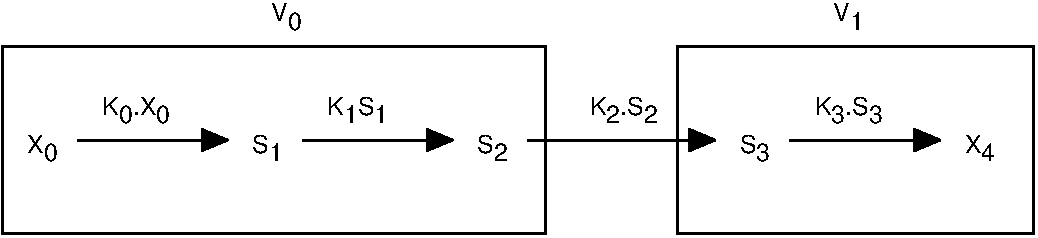
\includegraphics[scale=0.67]{multicomp}
  \caption{A example multi-compartmental model.}
  \label{fig:multicomp}
\end{figure}

Reaction equations are in substance per time units.  Species variables are in
concentrations.
Species $X_0$ and $X_4$ are boundary conditions.  The volume of compartment $V_1$
and the concentration of $X_0$ vary according to rules.

The SBML for this model is the following:

\begin{blockChanged}
\begin{small}
\tightspacing
\begin{verbatim}
<?xml version="1.0" encoding="UTF-8"?>
<sbml xmlns="http://www.sbml.org/sbml/level2/version2" level="2" version="2">
    <model id="ODEExampleModel">
        <listOfCompartments>
            <compartment id="V0" size="10"/>
            <compartment id="V1" size="1" constant="false"/>
        </listOfCompartments>
        <listOfSpecies>
            <species id="X0" initialConcentration="0" compartment="V0"
                boundaryCondition="true" />
            <species id="S1" initialConcentration="0" compartment="V0"/>
            <species id="S2" initialConcentration="0" compartment="V0"/>
            <species id="S3" initialConcentration="0" compartment="V1"/>
            <species id="X4" initialConcentration="0" compartment="V1"
                boundaryCondition="true" constant="true"/>
        </listOfSpecies>
        <listOfParameters>
            <parameter id="K0" value="0.1"/>
            <parameter id="K1" value="0.5"/>
            <parameter id="K2" value="0.1"/>
            <parameter id="K3" value="0.5"/>
            <parameter id="Kv" value="0.5"/>
            <parameter id="Kin" value="0.1"/>
        </listOfParameters>
        <listOfRules>
            <rateRule variable="X0">
                <math xmlns="http://www.w3.org/1998/Math/MathML">
                    <ci> Kin </ci>
                </math>
            </rateRule>
            <rateRule variable="V1">
                <math xmlns="http://www.w3.org/1998/Math/MathML">
                    <ci> Kv </ci>
                </math>
            </rateRule>
        </listOfRules>
        <listOfReactions>
            <reaction id="reaction_1" reversible="false">
                <listOfReactants>
                    <speciesReference species="X0"/>
                </listOfReactants>
                <listOfProducts>
                    <speciesReference species="S1"/>
                </listOfProducts>
                <kineticLaw>
                    <math xmlns="http://www.w3.org/1998/Math/MathML">
                        <apply>
                            <times/>
                            <ci> K0 </ci>
                            <ci> X0 </ci>
                         </apply>
                    </math>
                </kineticLaw>
            </reaction>
            <reaction id="reaction_2" reversible="false">
                <listOfReactants>
                    <speciesReference species="S1"/>
                </listOfReactants>
                <listOfProducts>
                    <speciesReference species="S2"/>
                </listOfProducts>
                <kineticLaw>
                    <math xmlns="http://www.w3.org/1998/Math/MathML">
                        <apply>
                            <times/>
                            <ci> K1 </ci>
                            <ci> S1 </ci>
                         </apply>
                    </math>
                </kineticLaw>
            </reaction>
            <reaction id="reaction_3" reversible="false">
                <listOfReactants>
                    <speciesReference species="S2"/>
                </listOfReactants>
                <listOfProducts>
                    <speciesReference species="S3"/>
                </listOfProducts>
                <kineticLaw>
                    <math xmlns="http://www.w3.org/1998/Math/MathML">
                        <apply>
                            <times/>
                            <ci> K2 </ci>
                            <ci> S2 </ci>
                         </apply>
                    </math>
                </kineticLaw>
            </reaction>
            <reaction id="reaction_4" reversible="false">
                <listOfReactants>
                    <speciesReference species="S3"/>
                </listOfReactants>
                <listOfProducts>
                    <speciesReference species="X4"/>
                </listOfProducts>
                <kineticLaw>
                    <math xmlns="http://www.w3.org/1998/Math/MathML">
                        <apply>
                            <times/>
                            <ci> K3 </ci>
                            <ci> S3 </ci>
                         </apply>
                    </math>
                </kineticLaw>
            </reaction>
        </listOfReactions>
    </model>
</sbml>
\end{verbatim}
\end{small}
\end{blockChanged}

The ODE translation of this model is as follows assuming all species variables
contain the species concentration:

Parameters and Constants:

\begin{equation*}
  \begin{array}{l}
    X_4 = 0 \\ \\[-4pt]
    V_0 = 10 \\ \\[-4pt]
    K_0 = 0.1\\ \\[-4pt]
    K_1 = 0.5\\ \\[-4pt]
    K_2 = 0.1\\ \\[-4pt]
    K_3 = 0.5\\ \\[-4pt]
    K_{in} = 0.1\\ \\[-4pt]
    K_v = 0.5\\ \\[-4pt]
  \end{array}
\end{equation*}

Initial Conditions of Variables:

\begin{equation*}
  \begin{array}{l}
    V_1 = 1 \\ \\[-4pt]
    X_0 = S_1 = S_2 = S_3 = 0
  \end{array}
\end{equation*}

Differential Equations:

\begin{equation*}
  \begin{array}{ll}
    \D\frac{d V_1}{d t} = K_v & \mbox{rule} \\ \\[-4pt]
    \D\frac{d X_0}{d t} = K_{in} & \mbox{rule} \\ \\[-4pt]
    \D\frac{d S_1}{d t} = \D\frac{K_0 X_0 - K_1 S_1}{V_0} & \mbox{reactions 1 and 2} \\ \\[-4pt]
    \D\frac{d S_2}{d t} = \D\frac{K_1 S_1 - K_2 S_2}{V_0} & \mbox{reactions 2 and 3} \\ \\[-4pt]
    \D\frac{d S_3}{d t} = \D\frac{K_2 S_2 - K_3 S_3}{V_1} & \mbox{reactions 3 and 4} \\ \\[-4pt]
  \end{array}
\end{equation*}


%-----------------------------------------------------------------------------
\subsection{Example Involving Function Definitions}
\label{sec:functioneg}
%-----------------------------------------------------------------------------

This section contains a model that uses the function definition
feature of SBML.  Consider the following hypothetical system:
\begin{equation*}
  \begin{array}{@{}ccc@{}}
    S_1 & \overset{\underrightarrow{f(S_1)}}{} & S_2 \\ \\[-4pt]
  \end{array}
\end{equation*}
where
\begin{equation*}
  \begin{array}{l}
    f(x) = x * 2 \\ \\[-4pt]
  \end{array}
\end{equation*}

The following is the XML document that encodes the model shown
above:

\begin{small}
\tightspacing
\begin{verbatim}
<?xml version="1.0" encoding="UTF-8"?>
<sbml xmlns="http://www.sbml.org/sbml/level2/version2" level="2" version="2">
    <model id="Example">
        <listOfFunctionDefinitions>
            <functionDefinition id="f">
                <math xmlns="http://www.w3.org/1998/Math/MathML">
                    <lambda>
                        <bvar><ci> x </ci></bvar>
                        <apply>
                            <times/>
                            <ci> x </ci>
                            <cn> 2 </cn>
                        </apply>
                    </lambda>
                </math>
            </functionDefinition>
        </listOfFunctionDefinitions>
        <listOfCompartments>
            <compartment id="compartmentOne" size="1"/>
        </listOfCompartments>
        <listOfSpecies>
            <species id="S1" initialConcentration="0" compartment="compartmentOne"/>
            <species id="S2" initialConcentration="0" compartment="compartmentOne"/>
        </listOfSpecies>
        <listOfReactions>
            <reaction id="reaction_1" reversible="false">
                <listOfReactants>
                    <speciesReference species="S1"/>
                </listOfReactants>
                <listOfProducts>
                    <speciesReference species="S2"/>
                </listOfProducts>
                <kineticLaw>
                    <math xmlns="http://www.w3.org/1998/Math/MathML">
                        <apply>
                            <ci> f </ci>
                            <ci> S1 </ci>
                         </apply>
                    </math>
                </kineticLaw>
            </reaction>
        </listOfReactions>
    </model>
</sbml>

\end{verbatim}
\end{small}

%-----------------------------------------------------------------------------
\subsection{Example Involving \emph{delay} Functions}
\label{sec:delayeg}
%-----------------------------------------------------------------------------

The following is a simple model illustrating the use of $delay$ to
represent a gene that suppresses its own expression.  The model can be
expressed in a single rule:
\begin{equation*}
\frac{d P}{d t} = \D\frac{ \D\frac{1}{1 + m (P_{delayed})^q} - P }{ \tau }
\end{equation*}
where
\begin{equation*}
\begin{array}{rl}
P_{delayed} & \mbox{is } delay(P, \Delta_t) \mbox{ or P at } t - \Delta_t\\
P & \mbox{is protein concentration}\\
\tau & \mbox{is the response time}\\
m & \mbox{is a multiplier or equilibrium constant}\\
q & \mbox{is the Hill coefficient}\\
\end{array}
\end{equation*}

The SBML form of this model is as follows:
\begin{blockChanged}
\begin{small}
\tightspacing
\begin{verbatim}
<?xml version="1.0" encoding="UTF-8"?>
<sbml xmlns="http://www.sbml.org/sbml/level2/version2" level="2" version="2">
    <model>
        <listOfCompartments>
            <compartment id="cell" size="1"/>
        </listOfCompartments>
        <listOfSpecies>
            <species id="P" compartment="cell" initialConcentration="0"/>
        </listOfSpecies>
        <listOfParameters>
            <parameter id="tau" value="1"/>
            <parameter id="m" value="0.5"/>
            <parameter id="q" value="1"/>
            <parameter id="delta_t" value="1"/>
        </listOfParameters>
        <listOfRules>
            <rateRule variable="P">
                <math xmlns="http://www.w3.org/1998/Math/MathML">
                 <apply>
                  <divide/>
                  <apply>
                   <minus/>
                   <apply>
                    <divide/>
                    <cn> 1 </cn>
                    <apply>
                     <plus/>
                     <cn> 1 </cn>
                     <apply>
                      <times/>
                      <ci> m </ci>
                      <apply>
                       <power/>
                       <apply>
                        <csymbol encoding="text"
                                 definitionURL="http://www.sbml.org/sbml/symbols/delay">
                            delay
                        </csymbol>
                        <ci> P </ci>
                        <ci> delta_t </ci>
                       </apply>
                       <ci> q </ci>
                      </apply>
                     </apply>
                    </apply>
                   </apply>
                   <ci> P </ci>
                  </apply>
                  <ci> tau </ci>
                 </apply>
                </math>
            </rateRule>
        </listOfRules>
    </model>
</sbml>
\end{verbatim}
\end{small}
\end{blockChanged}
%-----------------------------------------------------------------------------
\subsection{Example Involving Events}
\label{sec:eventeg}
%-----------------------------------------------------------------------------

This section presents a simple model system that demonstrates the use of
events in SBML.  Consider a system with two genes, $k_1$ and $k_2$.  $k_1$
is initially on and $k_2$ is initially off.  When turned on, the two genes
lead to the production of two products, $P_1$ and $P_2$, respectively, at a
fixed rate.  When $P_1$ reaches a given concentration, $k_2$ switches off.
This system can be represented mathematically as follows:
\begin{eqnarray*}
  \D\frac{d P_1}{d t} & = & k_1 - P_1\\[3pt]
  \D\frac{d P_2}{d t} & = & k_2 - P_2\\
  k_2 & = &
    \begin{cases}
      0 & \text{when $P_1 \leq \tau$},\\
      1 & \text{when $P_1 > \tau$}.
    \end{cases}
\end{eqnarray*}

The initial values are:
\begin{equation*}
  \begin{array}{lllll}
    k_1 = 1 & k_2 = 0 & \tau = 0.25 & P_1 = 0 & P_2 = 0\\ \\[-4pt]
  \end{array}
\end{equation*}

The SBML Level 2 representation of this as follows:

\begin{small}
\tightspacing
\begin{verbatim}
<?xml version="1.0" encoding="UTF-8"?>
<sbml xmlns="http://www.sbml.org/sbml/level2/version2" level="2" version="2"
      xmlns:math="http://www.w3.org/1998/Math/MathML">
    <model>
        <listOfCompartments>
            <compartment id="cell"/>
        </listOfCompartments>
        <listOfSpecies>
            <species id="P1" compartment="cell" initialConcentration="0"/>
            <species id="P2" compartment="cell" initialConcentration="0"/>
        </listOfSpecies>
        <listOfParameters>
            <parameter id="k1" value="1" constant="false"/>
            <parameter id="k2" value="0" constant="false"/>
            <parameter id="tau" value="0.25"/>
        </listOfParameters>
        <listOfRules>
            <rateRule variable="P1">
                <math:math>
                    <math:apply>
                        <math:minus/>
                        <math:ci> k1 </math:ci>
                        <math:ci> P1 </math:ci>
                    </math:apply>
                </math:math>
            </rateRule>
            <rateRule variable="P2">
                <math:math>
                    <math:apply>
                        <math:minus/>
                        <math:ci> k2 </math:ci>
                        <math:ci> P2 </math:ci>
                    </math:apply>
                </math:math>
            </rateRule>
        </listOfRules>
        <listOfEvents>
            <event>
                <trigger>
                    <math:math>
                        <math:apply>
                            <math:gt/>
                            <math:ci> P1 </math:ci>
                            <math:ci> tau </math:ci>
                        </math:apply>
                    </math:math>
                </trigger>
                <listOfEventAssignments>
                    <eventAssignment variable="k2">
                        <math:math>
                            <math:cn> 1 </math:cn>
                        </math:math>
                    </eventAssignment>
                </listOfEventAssignments>
            </event>
            <event>
                <trigger>
                    <math:math>
                        <math:apply>
                            <math:leq/>
                            <math:ci> P1 </math:ci>
                            <math:ci> tau </math:ci>
                        </math:apply>
                    </math:math>
                </trigger>
                <listOfEventAssignments>
                    <eventAssignment variable="k2">
                        <math:math>
                            <math:cn> 0 </math:cn>
                        </math:math>
                    </eventAssignment>
                </listOfEventAssignments>
            </event>
        </listOfEvents>
    </model>
</sbml>
\end{verbatim}
\end{small}

%-----------------------------------------------------------------------------
\subsection{Example Involving Two-Dimensional Compartments}
\label{sec:two-dimensional-eg}
%-----------------------------------------------------------------------------

The following example is a model that uses a two-dimensional compartment.
It is a fragment of a larger model of calcium regulation across the plasma
membrane of a cell.  The model includes a calcium influx channel,
\texttt{Ca\_channel}, and a calcium-extruding PMCA pump, \texttt{Ca\_Pump}.
The model also includes two cytosolic proteins that buffer calcium via the
\texttt{CalciumCalbindin\_gt\_BoundCytosol} and
\texttt{CalciumBuffer\_gt\_BoundCytosol} reactions.

\begin{small}
\tightspacing
\begin{verbatim}
<?xml version="1.0" encoding="UTF-8"?>
<sbml xmlns="http://www.sbml.org/sbml/level2/version2" level="2" version="2">
    <model id="facilitated_ca_diffusion">
        <listOfUnitDefinitions>
            <unitDefinition id="substance">
                <listOfUnits>
                    <unit kind="mole" scale="-6"/>
                </listOfUnits>
            </unitDefinition>
            <unitDefinition id="area">
                <listOfUnits>
                    <unit kind="metre" scale="-6" exponent="2" />
                </listOfUnits>
            </unitDefinition>
        </listOfUnitDefinitions>
        <listOfCompartments>
            <compartment id="Extracellular" spatialDimensions="3"/>
            <compartment id="PlasmaMembrane" outside="Extracellular" spatialDimensions="2"/>
            <compartment id="Cytosol" outside="PlasmaMembrane" spatialDimensions="3"/>
        </listOfCompartments>
        <listOfSpecies>
            <species
              id="CaBPB_C"
              compartment="Cytosol"
              initialConcentration="47.17"/>
            <species
              id="B_C"
              compartment="Cytosol"
              initialConcentration="396.04"/>
            <species
              id="CaB_C"
              compartment="Cytosol"
              initialConcentration="3.96"/>
            <species
              id="Ca_EC"
              compartment="Extracellular"
              initialConcentration="1000"/>
            <species
              id="Ca_C"
              compartment="Cytosol"
              initialConcentration="0.1"/>
            <species
              id="CaCh_PM"
              compartment="PlasmaMembrane"
              initialConcentration="1"/>
            <species
              id="CaPump_PM"
              compartment="PlasmaMembrane"
              initialConcentration="1"/>
            <species
              id="CaBP_C"
              compartment="Cytosol"
              initialConcentration="202.83"/>
        </listOfSpecies>
        <listOfReactions>
            <reaction id="CalciumCalbindin_gt_BoundCytosol" fast="true">
                <listOfReactants>
                    <speciesReference species="CaBP_C"/>
                    <speciesReference species="Ca_C"/>
                </listOfReactants>
                <listOfProducts>
                    <speciesReference species="CaBPB_C"/>
                </listOfProducts>
                <kineticLaw>
                           <notes>
                           <p xmlns="http://www.w3.org/1999/xhtml">
                               (((Kf_CalciumCalbindin_BoundCytosol * CaBP_C) * Ca_C) -
                                  (Kr_CalciumCalbindin_BoundCytosol * CaBPB_C))
                           </p>
                           </notes>
                    <math xmlns="http://www.w3.org/1998/Math/MathML">
                        <apply>
                            <minus/>
                            <apply>
                                <times/>
                                <ci> Kf_CalciumCalbindin_BoundCytosol </ci>
                                <ci> CaBP_C </ci>
                                <ci> Ca_C </ci>
                            </apply>
                            <apply>
                                <times/>
                                <ci> Kr_CalciumCalbindin_BoundCytosol </ci>
                                <ci> CaBPB_C </ci>
                            </apply>
                        </apply>
                    </math>
                         <listOfParameters>
                            <parameter id="Kf_CalciumCalbindin_BoundCytosol" value="20.0"/>
                            <parameter id="Kr_CalciumCalbindin_BoundCytosol" value="8.6"/>
                         </listOfParameters>
                </kineticLaw>
            </reaction>
            <reaction id="CalciumBuffer_gt_BoundCytosol" fast="true">
                <listOfReactants>
                    <speciesReference species="Ca_C"/>
                    <speciesReference species="B_C"/>
                </listOfReactants>
                <listOfProducts>
                    <speciesReference species="CaB_C"/>
                </listOfProducts>
                <kineticLaw>
                    <notes>
                      <p xmlns="http://www.w3.org/1999/xhtml">
                        (((Kf_CalciumBuffer_BoundCytosol * Ca_C) * B_C) -
                            (Kr_CalciumBuffer_BoundCytosol * CaB_C))
                      </p>
                    </notes>
                    <math xmlns="http://www.w3.org/1998/Math/MathML">
                        <apply>
                            <minus/>
                            <apply>
                                <times/>
                                <ci> Kf_CalciumBuffer_BoundCytosol </ci>
                                <ci> Ca_C </ci>
                                <ci> B_C </ci>
                            </apply>
                            <apply>
                                <times/>
                                <ci> Kr_CalciumBuffer_BoundCytosol </ci>
                                <ci> CaB_C </ci>
                            </apply>
                        </apply>
                    </math>
                    <listOfParameters>
                        <parameter id="Kf_CalciumBuffer_BoundCytosol" value="0.1"/>
                        <parameter id="Kr_CalciumBuffer_BoundCytosol" value="1.0"/>
                    </listOfParameters>
                </kineticLaw>
            </reaction>
            <reaction id="Ca_Pump">
                <listOfReactants>
                    <speciesReference species="Ca_C"/>
                </listOfReactants>
                <listOfProducts>
                    <speciesReference species="Ca_EC"/>
                </listOfProducts>
                <listOfModifiers>
                    <modifierSpeciesReference species="CaPump_PM"/>
                </listOfModifiers>
                <kineticLaw>
                    <notes>
                      <p xmlns="http://www.w3.org/1999/xhtml">
                        ((Vmax * kP * ((Ca_C - Ca_Rest) / (Ca_C + kP)) / (Ca_Rest + kP)) *
                            CaPump_PM)
                      </p>
                    </notes>
                    <math xmlns="http://www.w3.org/1998/Math/MathML">
                        <apply>
                            <divide/>
                            <apply>
                                <times/>
                                <ci> Vmax </ci>
                                <ci> kP </ci>
                                <ci> CaPump_PM </ci>
                                <apply>
                                    <minus/>
                                    <ci> Ca_C </ci>
                                    <ci> Ca_Rest </ci>
                                </apply>
                            </apply>
                            <apply>
                                <times/>
                                <apply>
                                    <plus/>
                                    <ci> Ca_C </ci>
                                    <ci> kP </ci>
                                </apply>
                                <apply>
                                    <plus/>
                                    <ci> Ca_Rest </ci>
                                    <ci> kP </ci>
                                </apply>
                            </apply>
                        </apply>
                    </math>
                    <listOfParameters>
                        <parameter id="Vmax" value="-4000"/>
                        <parameter id="kP" value="0.25"/>
                        <parameter id="Ca_Rest" value="0.1"/>
                    </listOfParameters>
                </kineticLaw>
            </reaction>
            <reaction id="Ca_channel">
                <listOfReactants>
                    <speciesReference species="Ca_EC"/>
                </listOfReactants>
                <listOfProducts>
                    <speciesReference species="Ca_C"/>
                </listOfProducts>
                <listOfModifiers>
                    <modifierSpeciesReference species="CaCh_PM"/>
                </listOfModifiers>
                <kineticLaw>
                    <notes>
                      <p xmlns="http://www.w3.org/1999/xhtml">
                        (J0 * Kc * (Ca_EC - Ca_C) / (Kc + Ca_C) * CaCh_PM)
                      </p>
                    </notes>
                    <math xmlns="http://www.w3.org/1998/Math/MathML">
                        <apply>
                            <divide/>
                            <apply>
                                <times/>
                                <ci> CaCh_PM </ci>
                                <ci> J0 </ci>
                                <ci> Kc </ci>
                                <apply>
                                    <minus/>
                                    <ci> Ca_EC </ci>
                                    <ci> Ca_C </ci>
                                </apply>
                            </apply>
                            <apply>
                                <plus/>
                                <ci> Kc </ci>
                                <ci> Ca_C </ci>
                            </apply>
                        </apply>
                    </math>
                    <listOfParameters>
                        <parameter id="J0" value="0.014"/>
                        <parameter id="Kc" value="0.5"/>
                    </listOfParameters>
                </kineticLaw>
            </reaction>
        </listOfReactions>
    </model>
</sbml>


\end{verbatim}
\end{small}

%-----------------------------------------------------------------------------
\subsection{Example using \class{SpeciesType} structures}
\label{sec:speciesType-eg}
%-----------------------------------------------------------------------------

The following example is a model that uses \class{SpeciesType} structures to indicate
that 2 pools of biochemical entities (\emph{species}) located in different compartments
contain the same type of entity (\emph{speciesType}).

\begin{small}
\tightspacing
\begin{verbatim}
<?xml version="1.0" encoding="UTF-8"?>
<sbml xmlns="http://www.sbml.org/sbml/level2/version2" level="2" version="2">
<model id="malate_aspartate_shuttle2">
    <listOfCompartments>
        <compartment id="Cytosol"/>
        <compartment id="Mitochondrial_Matrix"/>
    </listOfCompartments>
    <listOfSpeciesTypes>
        <speciesType id="Aspartate"/>
    </listOfSpeciesTypes>
    <listOfSpecies>
        <species
            id="Aspartate_in_Cytosol"
            speciesType="Aspartate"
            compartment="Cytosol"/>
        <species
            id="Aspartate_in_Mitochondrial_Matrix"
            speciesType="Aspartate"
            compartment="Mitochondrial_Matrix"/>
    </listOfSpecies>
</model>
</sbml>
\end{verbatim}
\end{small}


%=============================================================================
\section{Discussion}
\label{sec:discussion}
%=============================================================================

The volume of data now emerging from molecular biotechnology
leave little doubt that extensive computer-based modeling, simulation and
analysis will be critical to understanding and interpreting the
data~\citep{abbott:1999,gilman:2000,popel:1998,smaglik:2000}.  This
has lead to an explosion in the development of computer tools by many
research groups across the world.  The explosive rate of progress is
exciting, but the rapid growth of the field is accompanied by problems and
pressing needs.

One problem is that simulation models and results often cannot be directly
compared, shared or re-used, because the tools developed by different
groups often are not compatible with each other.  As the field of systems
biology matures, researchers increasingly need to communicate their results
as computational models rather than box-and-arrow diagrams.  They also need
to reuse published and curated models as library components in order to
succeed with large-scale efforts~\cite[e.g., the Alliance for Cellular
Signaling;][]{gilman:2000,smaglik:2000}.  These needs require that models
implemented in one software package be portable to other software packages,
to maximize public understanding and to allow building up libraries of
curated computational models.

We offer SBML to the systems biology community as a suggested format for
exchanging models between simulation/analysis tools.  SBML is an open model
representation language oriented specifically towards representing systems
of biochemical reactions.

Our vision for SBML is to create an open standard that will enable
different software tools to exchange computational models.  SBML is not
static; we continue to develop and experiment with it, and we interact with
other groups who seek to develop similar markup languages.  We plan on
continuing to evolve SBML with the help of the systems biology community to
make SBML increasingly more powerful, flexible and useful.


%=============================================================================
\subsection{Future Enhancements: SBML Level 3 and Beyond}
\label{sec:level-3}
%=============================================================================

As mentioned above, SBML Level 2 is intended to provide a foundation for
modeling biochemical networks.  Many people have expressed a desire to see
additional capabilities added to SBML.  The following summarizes additional
features that are under consideration to be included in SBML Level~3:
\begin{itemize}

\item \emph{Arrays}.  This will enable the creation of arrays of components
  (species, reactions, compartments and submodels).

\item \emph{Connections}.  This will be a mechanism for describing the
  connections between items in an array.

\item \emph{Geometry}.
This will enable the encoding of the spatial characteristics of models
including the geometry of compartments, the diffusion properties of species
and the specification of different species concentrations across different
regions of a cell.

\item \emph{Model Composition}.  This will enable a large model to be built up out
  of instances of other models.  It will also allow the reuse of model
  components and the creation of several instances of the same model.

\item \emph{Multi-state and Complex Species}.  This will allow the straight-forward
    construction of models involving species with a large number of states or
    species composed of subcomponents.  The representation scheme would be designed
    to contain the combinatorial explosion of objects that often results from these
    types of models.

%\item \emph{Controlled Vocabularies}.  This will enable models and model components
%to be labelled with instances of controlled vocabularies.  A model vocabulary
%will describe the SBML features used by a given model.

\item \emph{Diagrams}.  This feature will allow components to be
  annotated with data to enable the display of the model in a diagram.

\item \emph{Dynamic Structure}.  This will enable model structure to vary during simulation.
One aspect of aspect of this allowing
rules and reactions to have their effect conditional on the state of the model system.  For example in
SBML Level 2 it is possible to create a rule with the effect:
\begin{equation*}
\frac{d s}{d t} =
\left\{
\begin{array}{ll}
     0 & \mbox{if $s>0$}\\
     y & \mbox{otherwise}
\end{array}
\right.
\end{equation*}
Dynamic restructuring would enable the expression of the following example:
\begin{equation*}
\begin{array}{ll}
\mbox{if $s>0$} & \D\frac{d s}{d t} = y
\end{array}
\end{equation*}
where $s$ is not determined by the rule when $s \leq 0$.

%\item \emph{Rules for Initial Conditions}.  This will enable the encoding
%  of rules that are only executed at the start of a simulation i.e. set
%  initial conditions.  These rules will be similar to assignment rules and
%  are evaluated in the same sequence as assignment rules but only in the
%  very first instance of simulation.

\item \emph{Tie-breaking algorithm}.  This will include a controlled
  vocabulary and associated fields on models to indicate the
  simultaneous event tie-breaking algorithm required to correctly simulate
  the model.

%\item \emph{Composed Units}.  This will enable a unit definition to be
%composed from one or more other unit definitions.

\end{itemize}


%%=============================================================================
%\subsection{Relationships to Other Efforts}
%\label{sec:other-efforts}
%%=============================================================================

%There are a number of ongoing efforts with similar goals as those of SBML.
%Many of them are oriented more specifically toward describing protein
%sequences, genes and related entities for database storage and search.
%These are generally not intended to be computational models, in the sense
%that they do not describe entities and behavioral rules in such a way that
%a simulation package could ``run'' the models.

%The effort perhaps closest in spirit to SBML is
%CellML\tm~\citep{hedley:2001b}.  CellML is an XML-based markup language
%designed for storing and exchanging computer-based biological models.  It
%includes facilities for representing model structure, mathematics and
%additional information for database storage and search.  Models are
%described in terms of networks of connections between discrete components,
%where a component is a functional unit that may correspond to a physical
%compartment or simply a convenient modeling abstraction.  Components
%contain variables and connections contain mappings between the variables of
%connected components.  CellML provides facilities for grouping components
%and specifying the kinds of relationships that may exist between
%components.  It also uses MathML~\citep{w3c:2000b} for expressing
%mathematical relationships between components and provides the ability to
%use ECMAScript (formerly known as JavaScript) to define functions.

%The constructs in CellML tend to be at a more abstract and general level
%than those in SBML Level~2, and describe the structure and underlying
%mathematics of cellular models in a very general way.  By contrast, SBML is
%closer to the internal object model used in model analysis software.
%Because SBML Level~2 is being developed in the context of interacting with
%a number of existing simulation packages, it is a more concrete language
%than CellML and may be better suited to its purpose of enabling
%interoperability with existing simulation tools.

%The development of SBML Level 2 has benefited from discussions with the
%developers of CellML.  The developers of SBML and CellML are actively
%engaged in ensuring that the two representations can be translated between
%each other.


%%=============================================================================
%\subsection{Tracking the XML Schema Standard}
%\label{sec:tracking-xml}
%%=============================================================================

%One of the problems in attempting to define an XML Schema for SBML is that,
%at the time of this writing, the XML Schema
%specification~\citep{biron:2000,thompson:2000} has not actually been
%finalized.  This has been another motivation for defining SBML in terms of
%abstract data structures in a UML-based notation rather than directly as an
%XML Schema.

%The moving-target status of the XML Schema standard definition requires
%that we plan to update the Schema corresponding to SBML.  The following
%is our planned approach for handling changes in the Schema standard:
%\begin{enumerate}

%\item The definition of SBML Level~2 in this document is
%independent of XML
%  Schema.  Therefore, the definition of SBML Level~2 expressed here can
%  remain the same regardless of what happens to the exact form of XML
%  Schema.  Among other benefits, this allows developers to leave their
%  programs' internal data structures unchanged in the face of possible
%  revisions in the Schema standard.

%%\item In Appendix~\ref{apdx:schemas}, we provide an XML Schema
%%  corresponding to SBML Level~2 that has been created using the current
%%  definition of XML Schema from the W3C
%%  Organization~\citep{biron:2000,thompson:2000}.
%%
%\item Whenever the definition of XML Schema is updated by the W3C in the
%  future, we will issue a revised version of the XML Schema for SBML
%  Level~2 that conform to the updated standard.  We will leave the previous
%  versions still available for reference.  The updated XML Schemas for SBML
%  Level~2 will be identical to the previous versions except where changes
%  in XML Schema force a change in the definition of the Schema for SBML
%  Level~2.

%\end{enumerate}


%=============================================================================
\setcounter{secnumdepth}{-1}
\section{Acknowledgments}
\label{sec:acknowledgements}
%=============================================================================

\begin{blockChanged}
The development of SBML was originally funded entirely by the Japan Science
and Technology Agency (JST) under the ERATO Kitano Symbiotic Systems
Project.  The principal investigators were Hiroaki Kitano and John~C.
Doyle.  The original SBML Team was lead by Hamid Bolouri and included
Andrew Finney, Herbert Sauro, and Michael Hucka.

We gratefully acknowledge sponsorship from many funding agencies.  Support
for the continued development of SBML and associated software, meetings and
activities today comes from the following sources: the National Human
Genome Research Institute (USA); grant number GM070923 from the National Institute of General Medical
Sciences (USA); the International Joint Research Program of NEDO (Japan);
the JST ERATO-SORST Program (Japan); the Japanese Ministry of Agriculture;
the Japanese Ministry of Education, Culture, Sports, Science and
Technology; the BBSRC e-Science Initiative (UK); the DARPA IPTO
Bio-Computation Program (USA); and the Air Force Office of Scientific
Research (USA).  Additional support has been or continues to be provided by
the California Institute of Technology (USA), the University of
Hertfordshire (UK), the Molecular Sciences Institute (USA), and the Systems
Biology Institute (Japan).

SBML was first conceived at the JST/ERATO-sponsored \emph{First Workshop on
Software Platforms for Systems Biology}, held in April, 2000, at the
California Institute of Technology in Pasadena, California, USA.  The
participants collectively decided to begin developing a common XML-based
declarative language for representing models.  A draft version of the
Systems Biology Markup Language was developed by the Caltech ERATO team and
delivered to all collaborators in August, 2000.  This draft version
underwent extensive discussion over mailing lists and then again during the
\emph{Second Workshop on Software Platforms for Systems Biology} held in
Tokyo, Japan, November 2000.  A revised version of SBML was issued by the
Caltech ERATO team in December, 2000, and after further discussions over
mailing lists and in meetings, we produced a description of SBML
Level~1~\citep{hucka:2001}.  A journal publication~\citep{hucka:2003} was not produced until
much later, on the occasion of the development of Version~2 of
Level~1.

SBML Level~2 was conceived at the \emph{5th Workshop on Software Platforms
  for Systems Biology}, held in July 2002, at the University of
Hertfordshire, UK.  The participants collectively decided to revise the
form of SBML in Level~2.  The first draft of the Level~2 Version~1 document was released in
August 2002. The final set of features in SBML Level~2 Version~1 
was finalized in May 2003 at the \emph{7th Workshop on
  Software Platforms for Systems Biology} in Ft.\ Lauderdale, Florida.

SBML Level 2 Version~2 was developed with contributions from so many people
constituting the worldwide \emph{SBML Forum} that we regret it has become infeasible
to list individuals by name.  We are grateful to everyone on the
\texttt{sbml-discuss} and \texttt{libsbml-discuss} mailing lists, the
creators of CellML~\citep{hedley:2001b}, the members of the DARPA Bio-SPICE
project, and the authors of the following software SBML-aware systems:
BALSA,
BASIS,
BIOCHAM,
BioCharon,
biocyc2SBML,
BioGrid,
BioModels,
BioNetGen,
BioPathway Explorer,
Bio Sketch Pad,
BioSens,
BioSPICE Dashboard,
BioSpreadsheet,
BioTapestry,
BioUML,
BSTLab,
CADLIVE,
CellDesigner,
Cellerator,
CellML2SBML,
Cellware,
CL-SBML,
COPASI,
Cytoscape,
DBsolve,
Dizzy,
E-CELL,
ecellJ,
ESS,
FluxAnalyzer,
Fluxor,
Gepasi,
INSILICO discovery,
JACOBIAN,
Jarnac,
JDesigner,
JigCell,
JWS Online,
Karyote,
KEGG2SBML,
Kinsolver,
libSBML,
MathSBML,
MesoRD,
MetaboLogica,
MetaFluxNet,
MMT2,
Modesto,
Moleculizer,
Monod,
Narrator,
NetBuilder,
Oscill8,
PANTHER Pathway,
PathArt,
PathScout,
PathwayLab,
Pathway Tools,
PathwayBuilder,
PATIKAweb,
PaVESy,
PET,
PNK,
Reactome,
ProcessDB,
PROTON,
pysbml,
PySCeS,
runSBML,
SABIO-RK,
SBML ODE Solver,
SBMLeditor,
SBMLmerge,
SBMLR,
SBMLSim,
SBMLToolbox,
SBliD,
SBToolbox,
SBW,
SCIpath,
Sigmoid,
SigPath,
SigTran,
SIMBA,
SimBiology,
Simpathica,
SimWiz,
SmartCell,
SRS Pathway Editor,
StochSim,
STOCKS,
TERANODE Suite,
Trelis,
Virtual Cell,
WinSCAMP,
and
XPPAUT.


\end{blockChanged}

%BASIS, BioSketchPad, BioSpice, CellDesigner, Cellerator, CellML,
%COPASI, DBSolve, E-Cell, ESS, Gepasi, Jarnac, JDesigner, JigCell, MCell,
%NetBuilder, Promot/DIVA, StochSim, and Virtual Cell, and members of the
%\texttt{sysbio} and \texttt{sbml-discuss} mailing lists.  We are
%particularly grateful to the following people for discussions, advice and
%comments: Nicolas Allen, Adam Arkin, Hamid Bolouri, Ben Bornstein, Dennis
%Bray, Roger Brent, Steve Burbeck, Claudine Chaouiya, Kwang Cho, Athel
%Cornish-Bowden, Manuel Corpas, Autumn Cuellar, John Doyle, Serge Dronov,
%Drew Endy, David Fell, Carl Firth, Ed Frank, Akira Funahashi, Ralph Gauges,
%Martin Ginkel, Victoria Gor, Igor Goryanin, Warren Hedley, Charles Hodgman,
%Stefan Hoops, Nick Juty, Jay Kaserger, Sarah Keating, Hiroaki Kitano, Ben
%Kovitz, Andreas Kremling, Nicolas Le~Nov\`{e}re, Fred Livingston, Les Loew,
%Daniel Lucio, Joanne Matthews, Mike McCollum, Pedro Mendes, Eric Minch,
%Eric Mjolsness, David Morley, Mineo Morohashi, Poul Nielsen, Greg Peterson,
%Mark Poolman, Carole Proctor, Wayne Rindone, Sven Sahle, Takeshi Sakurada,
%Vijay Saraswat, Herbert Sauro, James Schaff, Maria Schilstra, John Schwacke,
%Cliff Shaffer, Bruce Shapiro, Tom Shimizu, Herbert Sauro, Hugh Spence,
%J\"{o}rg Stelling, Kouichi Takahashi, Masaru Tomita, Marc Vass, John Wagner,
%Jonathan Webb, J\"{o}rg Weimar, Darren Wilkinson, Olaf Wolkenhauer and Tau-Mu Yi.


%\changed{Both versions of SBML Level 2 were} created in
%collaboration with the authors of the following systems:
%\emph{BASIS}~\citep{kirkwood:2003},
%\emph{Bio Skektch Pad}~\citep{belta:2003},
%\emph{BioSpreadsheet}~\citep{mccollum_2003},
%\emph{BioSpice}~\citep{arkin:2001},
%\emph{CellDesigner}~\citep{funahashi:2003},
%\emph{Cellerator}~\citep{shapiro:2001,shapiro:2003b},
%\emph{COPASI}~\citep{mendes:2000},
%\emph{DBsolve}~\citep{goryanin:2001,goryanin:1999},
%\emph{E-CELL}~\citep{tomita:1999,tomita:2001},
%\emph{ESS}~\citep{peterson:2003},
%\emph{Gepasi}~\citep{mendes:1997,mendes:2001},
%\emph{Jarnac}~\citep{sauro:2000,sauro:1991},
%\emph{JDesigner}~\citep{sauro:2001b},
%\emph{JigCell}~\citep{vass:2003},
%\emph{MCell}~\citep{bartol:2002},
%\emph{NetBuilder}~\citep{schilstra:2002},
%\emph{PathScout}~\citep{minch_2003},
%\emph{ProMoT/DIVA}~\citep{stelling:2001},
%\emph{StochSim}~\citep{bray:2001,morton-firth:1998}, and
%\emph{Virtual Cell}~\citep{schaff:2000,schaff:2001}.
%\changed{Both versions of SBML Level 2 were} developed with the help of these
%packages' authors, as well as help and collaboration from the
%creators of CellML~\citep{hedley:2001b} and many other individuals
%listed in the Acknowledgments
%(Section~\ref{sec:acknowledgements}).



\newpage
\section{Appendix}
\setcounter{secnumdepth}{2}
\appendix

%-----------------------------------------------------------------------------
\section{\changed{Differences between SBML Level 1 Version 2 and Level 2 Version 1}}
%-----------------------------------------------------------------------------
\label{apdx:level1-level2}

\changed{Compared to SBML Level 1 Version 2, SBML Level 2 Version
1 introduces the following changes:}
\begin{itemize}

\item SBML Level 2 supports the inclusion of metadata using the same approach as
  CellML~\citep{cuellar:2002}.  All structures in SBML can be annotated
  with optional content in RDF~\cite[Resource Description
  Format;][]{lassila:1999} following the guidelines put forward by
  \citeauthor{cuellar:2002}. (Section~\ref{sec:sbase}.)

\item All data structures, including \class{Sbml} and
  \class{listOf}\rule{0.5in}{0.5pt} elements, are now derived from the type
  \class{SBase}.  (Section~\ref{sec:sbase}.)  This means all major
  structures in SBML can have separate annotations and metadata associated
  with them.

\item A new field, \attrib{id}, replaces the \attrib{name} field previously
  defined for most SBML structures to identify each part of a model.  (See
  Section~\ref{sec:idnameattribs}.)  The \attrib{id} field has a type of
  \class{SId}, whose definition is similar to \class{SName} in Level~1.  In
  SBML Level~2, the \attrib{name} field is optional and is defined to allow
  any Unicode characters allowed by the \class{string} type of XML
  Schema~\citep{biron:2000}.

\item Formulas in Level~2 are expressed using MathML~\citep{w3c:2000b} 2.0.
  The field named \attrib{formula} previously available on the
  \class{KineticLaw} and \class{Rule} structures has been replaced by a
  MathML element named \class{math} containing MathML content.  In
  addition, stoichiometry numbers may now be expressed using MathML,
  allowing for more flexibility in defining reactions.
  (Sections~\ref{sec:formulas}, \ref{sec:rules} and~\ref{sec:reactions}.)

\item The namespace for identifiers in a model does not contain any
  built-in symbols; gone, for example, are the predefined rate laws of SBML
  Level~1.  The approach taken in SBML Level~2 is that each model must
  itself define whatever functions it needs using the new
  \class{FunctionDefinition} mechanism.  Although SBML Level~2 \emph{does}
  define two built-in entities (a symbol representing time and another
  symbol representing delay functions), these are referenced using a
  feature of MathML and are not in the same namespace as identifiers
  defined by a model.  (Section~\ref{sec:csymbol-token}.)

\item SBML Level~2 makes explicit a previously unstated assumption, that
  the XML encoding of a model uses UTF-8.  SBML documents must refer to the
  UTF-8 encoding in their XML declaration.  (Section~\ref{sec:sbml}.)

\item The top-level \class{Model} structure can contain an optional list of
  global user-defined functions expressed in MathML and organized in new
  structures of type \class{FunctionDefinition}.  (Sections~\ref{sec:model}
  and \ref{sec:functions}.)

\item The top-level \class{Model} structure can contain an optional list of
  event definitions organized in structures of type \class{Event}.  Events
  define discrete changes in model behavior at specific times during a time
  simulation of the model.  (Section~\ref{sec:model} and \ref{sec:events}.)

\item Unlike in SBML Level~1, unit identifiers in Level~2 are in a separate
  namespace from the namespace used for models, functions, species,
  compartments, reactions and parameters.  Also, the unit names
  ``\unit{meter}'' and ``\unit{liter}'' are not defined in Level~2 because
  the SBML user community deemed them unnecessary.  Finally, \class{Unit}
  structures now have the additional fields \attrib{multiplier} and
  \attrib{offset} to enable the definition of non-SI units.
  (Section~\ref{sec:unitdefinitions}.)

\item The \class{Compartment} structure has a new field,
  \attrib{spatialDimensions}, whose value is a positive integer specifying
  the number of dimensions in space the compartment possesses.  This
  enables the definition of such things as two-dimensional membranes.  As a
  side-effect, the units of species concentration in SBML Level~2 depend on
  the spatial dimensions of the compartment where the species is located.
  To support these new capabilities, \attrib{Compartment} now uses a field
  named \attrib{size} instead of \attrib{volume}, and there are two new
  built-in units for area and length.  (Sections~\ref{sec:unitdefinitions}
  and \ref{sec:compartments}.)

\item All fields representing initial conditions or parameter values,
  including compartment sizes and species concentrations, are optional in
  Level~2.  A missing value for one of these fields implies that the value
  is either unknown, not required for analysis, or should be obtained from
  an external source. (Sections~\ref{sec:compartments}, \ref{sec:species}
  and \ref{sec:parameters}.)

\item The \class{Compartment}, \class{Species} and \class{Parameter}
  structures each have a new boolean field named \attrib{constant}.  This
  field specifies whether the variables represented by these structures can
  be changed by rules and reactions.  (Sections~\ref{sec:compartments},
  \ref{sec:species} and~\ref{sec:parameters}.)

\item The \class{Species} structure has a new field,
  \attrib{initialConcentration}, for setting the initial value of a species
  in terms of its concentration.  This is in addition to the ability,
  carried over from Level~1, to set the values in terms of amounts.
  (Section~\ref{sec:species}.)

\item The \class{Species} structure has two new fields, \attrib{spatialSizeUnits}
  and \attrib{substanceUnits}, which replace the \attrib{units} field in Level~1.
  These fields are composed to form the concentration units of the species
  symbol.  (Section~\ref{sec:species}.)

\item The rule structures are simpler compared to SBML Level~1.
\changed{There is
  no longer a \attrib{type} field on \class{AssignmentRule}.  A redesigned structure
  \class{AssignmentRule} and new \class{RateRule} structure replace SBML Level~1's
  \class{ParameterRule}, \class{SpeciesConcentrationRule} and
  \class{CompartmentVolumeRule}.}  (Section~\ref{sec:rules}.)

\item The \class{Reaction} structure has a new list of \emph{modifiers} in
  addition to the list of reactants and products.  The
  \attrib{listOfModifiers} enumerates species that affect a reaction but
  are neither created nor destroyed by the reaction.
  (Section~\ref{sec:reactions}.)

\end{itemize}

%-----------------------------------------------------------------------------
\begin{blockChanged}
\section{Differences between SBML Level 2 Version 1 and Level 2 Version 2}
%-----------------------------------------------------------------------------
\label{apdx:version1-version2}

The changes introduced by SBML Level 2 Version 2 over Level 2
Version 1 as described by this specification are divided into 2
parts: (a) new features and (b) Version 1 errata corrected in
Version 2.

The new features introduced in Version 2 are:

\begin{itemize}

\item \emph{XML namespace}

The XML namespace for SBML Level 2 Version 2 is
\url{http://www.sbml.org/sbml/level2/version2}.

\item \emph{Removal of predefined annotation namespaces}

In Section~\ref{sec:annotation-use}, previous Levels and Versions
of SBML reserved a set of XML Namespace names corresponding to
software tools known to exist at the time.  Due to the explosion
of SBML-compatible software tools in recent years, it has become
infeasible to maintain such a list; moreover, informal discussions
with SBML users revealed that no one paid much attention to the
list anyway.  Beginning with SBML Level~2 Version~2, no such
namespaces are defined in the SBML specification.

\item \emph{One top level element per XML Namespace per
\class{annotation} element and associated restrictions}

An \class{annotation} element cannot contain two or more top level
elements in the same XML namespace.  An \class{annotation} element
cannot contain a top level element in the SBML namespace.  The
order of top level elements within an \class{annotation} element
is not significant.

\item \emph{sboTerm}

In Version 2 \class{SimpleSpeciesReference},
\class{InitialAssignment}, \class{KineticLaw}, \class{Parameter},
\class{Reaction}, \class{Model}, \class{Rule} and
\class{Constraint} structures have an addition field
\attrib{sboTerm}.  These fields can only contain valid Systems
Biology Ontology (SBO) \sboref term values (that is they are of
type SBOTerm).

\item \emph{New format for linking external resources to SBML}

A new format for using RDF and Dublin Core within
\class{annotation} elements to link SBML models to external
resources and record model version history is introduced. Whilst
CellML metadata can be included in SBML the specification does not
make any specific mention of CellML metadata.

\item \emph{Built-in units can be dimensionless}

In Version 2 the built-in units, e.g. \emph{substance} and
\emph{volume}, can be assigned \emph{dimensionless} units. This
facilities the correct encoding of models based on dimensionless
experimental data.

\item \emph{Substance units can be mass derived}

\emph{FIX ME - this needs to be sorted out}

In Version 2 the \emph{substance} built-in unit can be derived
directly from kilogram rather from mole.  This facilitates the
correct encoding of models that use a mass based rather mole based
units system (see \citep{domach:2000, castellanos:2004} for
examples of such models).

\item \emph{Compartment Type}

In Version 2 the \class{Model} structure has an addition list of
\class{CompartmentType} structures.  Each of these structures
represents a type of compartment and consists of just
\attrib{name} and \attrib{id} fields.  The \attrib{id} field can
optionally be referenced from an \class{Compartment} structure
using a new \attrib{compartmentType} field.

\item \emph{Species Type}

In Version 2 the \class{Model} structure has an addition list of
\class{SpeciesType} structures.  A \class{SpeciesType} structure
represents a type of chemical entity independent of location and
consists of just \attrib{name} and \attrib{id} fields.  The
\attrib{id} field can optionally be referenced from an
\class{Species} structure using a new \attrib{speciesType} field.

\item \emph{\attrib{charge} field deprecated}

In Version 2 the \class{Species} structure \attrib{charge} field
is deprecated.

\item \emph{Constraint}

In Version 2 the \class{Model} structure has an addition list of
\class{Constraint} structures.  The \attrib{math} field of
\class{Constraint} contains a boolean expression which is is
function of the model state which returns whether the state is
valid.  Unlike the \class{Rule} structures \class{Constraint}
should not be used to compute the dynamical behavior of the model.

\item \emph{\attrib{Id} on \class{SimpleSpeciesReference}}

Version 2 adds \attrib{id} and \attrib{name} fields to the
\class{SimpleSpeciesReference} structure.  The \class{id} field
declares an identifier which is in the global namespace of
objects.

\item \emph{Reaction identifier as a symbol in math expressions}

In Version 2 the value of the \attrib{id} of any reaction can
appear in an expression within a MathML \class{ci} element.  The
symbol represents the rate of the reaction which is given by the
\class{KineticLaw} structure of the \class{Reaction}.  It is not
possible to explicitly assign a value to the symbol using
\class{InitialAssignment}, \class{EventAssignment},
\class{AssignmentRule} or \class{RateRule} structures.

\item \emph{Initial Assignment Structures}

In Version 2 the \class{Model} structure has an additional list of
\class{InitialAssignment} structures.  This list of structures is
evaluated before an reactions or other rules to determine the
values of constants and the initial values of variables.
Assignment rules override the values calculated by the
\class{InitialAssignment} structures.

\item \emph{The order of \class{AssignmentRule} structures is not
significant}

In Version 2 the order of \class{AssignmentRule} is not
significant however the set of assignment rules formed from
\class{KineticLaw}, \class{InitialAssignment} and
\class{AssignmentRule} structures as a whole must not contain
algebraic loops.

\end{itemize}

The errata in the SBML Level 2 Version 1 specification that
corrected in this Version 2 specification are as follows.  The
page and section numbers refer to the final PDF version of the
SBML Level 2 Version 1 specification.

\begin{itemize}

\item page 1: The specification should contain a link to the
latest version of the specification and to this specific
\emph{issue} of the document.

\item page 2: Each additional errata to the specification should
result in an new issue of the specification each with a unique
number.  The first issue of the specification should be numbered
1.  The errata on this specification should recorded in a new
section starting in issue 2.  Each errata will be numbered with
the issue in which the errata is introduced.  Errata should not
change the fundamental semantics or syntax of SBML but merely
clarify and disambiguate the specification.

%\item page 2: Each new level, version and issue of SBML should be
%announced on a low volume emailing list mentioned in the
%specification.

\item page 2: The specification should make explicit the features
which are not backwards compatable between Level 2 Version 2 and
Level 2 Version 1.

\item page 3 Section 1.2: The specification should make explicit
the differences in the numeric types of XML Schema and MathML.

\item page 4 Section 3.1: This section should include an
explanation of why \attrib{id} and \attrib{name} fields are not
present on \class{SBase}.

\item page 8 Figure 3: Change \texttt{nameChar} and \texttt{name}
to \texttt{idChar} and \texttt{SId} to indicate clearly the use of
the BNF syntax definition.

\item page 9 Section 3.6: The specification should reference
existing documents to clarify the semantics of the MathML
operators in the MathML subset.

\item page 9 Section 3.6: The specification should constrain the
use of MathML operators which return different types of result
(numeric or boolean) appropriately.

\item page 9 Section 3.6.1: The \attrib{encoding} attribute is
permitted on MathML \class{annotation} and
\\ \class{annotation-xml} elements, not only on \class{csymbol} as
stated on that page.

\item page 9 Section 3.6.1: The MathML standard specifies the
result of n-ary operators when the number of operands is
critically small, for example for \class{times} and \class{add}
elements, when the number of operands are zero or one.  This is an
obscure part of MathML and the specification should highlight the
relevant sections of the MathML specification.

\item page 9 Section 3.6.2: The specification should make explicit
the differences in the numeric types of XML Schema and MathML.

\item page 9 Section 3.6.2: The specification should describe the
MathML whitespace rules for \class{cn} elements.

\item page 10 Section 3.6.3: The specification should describe the
MathML whitespace rules for \class{ci} elements.

\item page 10 Section 3.6.3: The specification should state
whether SBML has early or late binding semantics.

\item page 10, Section 3.6.4: The delay function is not clearly
defined. There is no explanation of what range of values is valid
for the time.  For example, can delay times be less than zero?
Also, are there restrictions on the acceptable values of the
argument $x$?

\item page 13, Section 4.3.1: The `can' in the second sentence
should be replaced by `should'.

\item page 14, Section 4.4.2: The \attrib{id} field of a
\class{UnitDefinition} structure must not contain a value from
Table 2, the table of \class{UnitKind} values.  This restriction
is necessary because otherwise a unit definition could redefine
one of the base unit kinds.

\item page 14, Section 4.4.2: The first formula should be the
following:
\begin{equation*}
u_{new} = (\emph{multiplier} \times 10^{\emph{scale}} \times
u)^{\emph{exponent}} + \emph{offset}
\end{equation*}  This equation is superseded by modifications
to the \class{Unit} structure in this specification (SBML Level 2
Version 2).

\item page 16, Section 4.4.3: The example code redefining the
built-in unit \texttt{volume} should replace \texttt{liters} with
\texttt{litre}. \texttt{liters} is not a valid value for the
\attrib{kind} attribute.

%\item page 17 Section 4.5.5 and page 19 Section 4.6.4: The text is
%slightly contradictory.  The text needs to be improved.

\item page 18 section 4.5.6: the value of \attrib{outside} field
for a given \class{Compartment} structure must be the value of an
\attrib{id} field of another \class{Compartment} structure.

\item page 18 Section 4.5.6: The graph formed where compartments
are nodes and the arcs are implied by the values of
\attrib{outside} attributes must be acyclic otherwise a
compartment can be outside itself.

\item page 19 Section 4.6.3: On \class{Species} elements the
\attrib{initialConcentration} attribute can have a value even if
the \attrib{hasOnlySubstanceUnits} attribute is ``\texttt{true}''.

\item page 19 Section 4.6.4: This section should contain a table
that shows how the units of a species is determined from the
spatial dimensions of the species and the value of the
\attrib{hasOnlySubstanceUnits} attribute.

\item page 24 Section 4.8.4: This section should specify that the
model should not be overdetermined as defined in
Section~\ref{sec:ruleconstraints} of the SBML Level 2 Version 2
specification (i.e. this document).

\item page 24 Section 4.8.4: This section should not refer to
assignment rules using the term `scalar rule'.

\item page 27 Section 4.9.5: If a species id occurs in any
\class{ci} element MathML element including \class{KineticLaw} and
\class{StoichiometryMath} elements it should appear in a
\class{SimpleSpeciesReference} element in the reaction.  The
specification only applies this rule to the \class{KineticLaw}
element. Such a species is at a minimum a modifier of the
reaction.

\item page 29 Section 4.9.5: The relationship of the abstract
class \class{SimpleSpeciesReference} to the concrete classes
\class{SpeciesReference} and \class{ModifierSpeciesReference}
should be made explicit.

\item page 29 Section 4.9.6: Despite being redundant it is
possible for a species to be referenced from the \attrib{modifier}
field whilst being referenced from the \attrib{product} and/or
\attrib{reactant} fields of the same reaction.

\item page 29 section 4.9.7: 3rd paragraph: The text is overly
restrictive and contradictory with respect of the units of species
symbols. Species symbols can be either amount or concentration
units depending on the species declaration.

\item page 29 section 4.9.7: Final paragraph: The kinetic law
expression is composed so that the units are of the parameter are
not those conventionally used.  This is not good practice.  The
rate law expression should be changed to include the compartment
volume so that the units of the parameter are those that would be
measured by an experimentalist and used in practice by a modeler.

\item page 31 Section 4.10.5: A \attrib{variable} attribute on a
\class{EventAssignment} element should be unique among the set of
assignments within an \class{Event} element if not the effect of
event assignment is ambiguous.

\item page 31 Section 4.10.5: A \attrib{variable} attribute on a
\class{EventAssignment} element should not have the same value as
a \attrib{variable} attribute on a \class{AssignmentRule} element.

\item page 32 Section 4.10.7: \emph{Any} transition of a
\attrib{trigger} expression from false to true will cause an
\class{event} to \emph{fire}.  Consider an \class{event} $E$ with
delay $d$ where the \attrib{trigger} expression makes a transition
from false to true at times $t_1$ and $t_2$.  The
\class{EventAssignment} structure will have effect at $t_1+d$ and
$t_2+d$ irrespective of the relative times of $t_1$ and $t_2$. For
example events can ``overlap'' so that $t_1 < t_2 < t_1+d$ still
causes event assignments to occur at $t_1+d$ and $t_2+d$.

\item page 32 Section 4.10.7: Events cannot be triggered at $t=0$.

\item page 34 Section 5.2: The units of parameter \texttt{Km}
should be moles per litre as the parameter is added to the
concentration of a species.

\item page 38 Example 5.3: The \texttt{out} reaction should have a
\class{listOfModifiers} which refers to species \texttt{S2} since
it is referenced in the reaction's \class{KineticLaw}.

\item page 40 Example 5.5: The one rule in \class{listOfRules}
should not use \texttt{<apply> ... </apply>}; these tags should be
omitted.

\item page 42 Example 5.6: The MathML in the two \class{RateRule}
definitions should not use \texttt{<apply> ... </apply>}; these
tags should be omitted.

\item page 46 Example 5.8: The \attrib{definitionURL} attribute
value for the \class{csymbol} delay should be
\\ \texttt{http://www.sbml.org/sbml/symbols/delay}, not
\texttt{http://www.sbml.org/symbols/delay} (the incorrect form has
``sbml'' omitted).

\item page 55 Appendix A: The appendix states that UML inheritance
is mapped, in XML Schema, to the \texttt{extension} of
\class{complexType} elements. This is by far the most natural
interpretation and the one used in the schema available on the
SBML web site and used by libSBML. However, this approach
introduced a restriction: an ordering of elements is imposed on
all extended types because the definition of XML Schema
effectively requires the use of \texttt{sequence} ordering in
order to be able to use type inheritance in this way. (A full
explanation of the details can be found in Section 13.5 of
~\cite{walmsley:2002} ) The result is that the ordering of
subelements in SBML XML is important.  For example, \class{notes}
and \class{annotation} elements must occur before
\class{listOfReactants} elements within a \class{Reaction}
element. Appendix A should state this restriction explicitly.
Appendix A should be moved into the main text.  The dependence on
\texttt{sequence} is a result of using XML Schema.

\item page 55 Appendix A: The SCHUCS document doesn't state what
model group element should be used in the XML schema
interpretation of UML. (Examples of XML schema are that
\class{xs:element} elements should be enclosed in
\class{xs:choice}, \class{xs:all} or \class{xs:sequence} elements;
see p.488 table A-1 of~\cite{walmsley:2002}.) To be consistent
with the previous errata item, \class{xs:sequence} elements should
be used.  (The SBML schemas use this interpretation).

\item page 56, Appendix B: The last bullet, second sentence
starts: ``there is no longer a \attrib{type} field on
\class{Rule}''. Technically, this should read: ``there is no
longer a \attrib{type} field on \class{AssignmentRule}''.

\end{itemize}

\end{blockChanged}
%=============================================================================
\section{XML Schema for SBML}
\label{apdx:schema}
%=============================================================================

The following is an XML Schema definition for the SBML Level 2
Version 1, using the W3C Recommendation for XML Schema version 1.0
of 2 May 2001~\citep{biron:2000,fallside:2000,thompson:2000}. This
schema does not define all aspects of SBML Level 2: a SBML
document validated by this schema is not necessarily a valid SBML
Level 2 document.  Appendix~\ref{apdx:mathml-subset-schema}
contains a a schema for the SBML MathML subset.
Appendix~\ref{apdx:validation-rules} contains a list of the
remaining checks required to validate a model that is already
consistent with these two schemas.

\begin{small}
\tightspacing
\begin{verbatim}
<?xml version="1.0" encoding="UTF-8"?>
<xsd:schema
    targetNamespace="http://www.sbml.org/sbml/level2/version2"
    xmlns="http://www.sbml.org/sbml/level2/version2"
    xmlns:mml="http://www.w3.org/1998/Math/MathML"
    xmlns:xlink="http://www.w3.org/1999/xlink"
    xmlns:xsi="http://www.w3.org/2001/XMLSchema-instance"
    xmlns:xsd="http://www.w3.org/2001/XMLSchema"
    elementFormDefault="qualified"
    attributeFormDefault="unqualified"
    version="SBML L2 V2">
    <xsd:import
        namespace="http://www.w3.org/1998/Math/MathML"
        schemaLocation="http://www.w3.org/Math/XMLSchema/mathml2/mathml2.xsd"/>
    <xsd:annotation>
        <xsd:documentation>
      File name : sbml.xsd
      Author : M. Hucka, A. Finney, D. Lucio
\end{verbatim}
\begin{blockChanged}
\begin{verbatim}
      Description : XML Schema for the Systems Biology Markup Language Level 2 Version 2
                    This is designed for XML Schema version 1.0.
      Version : 1

      Copyright 2006 California Institute of Technology and Japan Science and
      Technology Corporation.
\end{verbatim}
\end{blockChanged}
\begin{verbatim}

      This library is free software; you can redistribute it and/or modify it
      under the terms of the GNU Lesser General Public License as published
      by the Free Software Foundation; either version 2.1 of the License, or
      any later version.

      This file is distributed in the hope that it will be useful, but
      WITHOUT ANY WARRANTY, WITHOUT EVEN THE IMPLIED WARRANTY OF
      MERCHANTABILITY OR FITNESS FOR A PARTICULAR PURPOSE.  The software
      and documentation provided hereunder is on an "as is" basis, and the
      California Institute of Technology and Japan Science and Technology
      Corporation have no obligations to provide maintenance, support,
      updates, enhancements or modifications.  In no event shall the
      California Institute of Technology or the Japan Science and Technology
      Corporation be liable to any party for direct, indirect, special,
      incidental or consequential damages, including lost profits, arising
      out of the use of this software and its documentation, even if the
      California Institute of Technology and/or Japan Science and Technology
      Corporation have been advised of the possibility of such damage.  See
      the GNU Lesser General Public License for more details.

      You should have received a copy of the GNU Lesser General Public License
      along with this library; if not, write to the Free Software Foundation,
      Inc., 59 Temple Place, Suite 330, Boston, MA 02111-1307 USA.
</xsd:documentation>
    </xsd:annotation>
    <!--The definition of SId follows.-->
    <xsd:simpleType name="SId">
        <xsd:annotation>
            <xsd:documentation>
                The type SId is used throughout SBML as the type of the 'id'
                attributes on model elements.
            </xsd:documentation>
        </xsd:annotation>
        <xsd:restriction base="xsd:string">
            <xsd:pattern value="(_|[a-z]|[A-Z])(_|[a-z]|[A-Z]|[0-9])*"/>
        </xsd:restriction>
    </xsd:simpleType>
\end{verbatim}
\begin{blockChanged}
\begin{verbatim}
    <xsd:simpleType name="SBOTerm">
        <xsd:annotation>
            <xsd:documentation>a string for referring to an SBO term</xsd:documentation>
        </xsd:annotation>
        <xsd:restriction base="xsd:string">
            <xsd:pattern value="(SBO:)([0-9]{7})"/>
        </xsd:restriction>
    </xsd:simpleType>
\end{verbatim}
\end{blockChanged}
\begin{verbatim}
    <!--The definition of SBase follows.-->
    <xsd:complexType name="SBase" abstract="true">
        <xsd:annotation>
            <xsd:documentation>
                The SBase type is the base type of all main components in SBML.
                It supports attaching metadata, notes and annotations to components.
            </xsd:documentation>
        </xsd:annotation>
        <xsd:sequence>
            <xsd:element name="notes" minOccurs="0">
                <xsd:complexType>
                    <xsd:sequence>
                        <xsd:any
                            namespace="http://www.w3.org/1999/xhtml"
                            processContents="skip"
                            minOccurs="0"
                            maxOccurs="unbounded"/>
                    </xsd:sequence>
                </xsd:complexType>
            </xsd:element>
            <xsd:element name="annotation" minOccurs="0">
                <xsd:complexType>
                    <xsd:sequence>
                        <xsd:any processContents="skip" minOccurs="0" maxOccurs="unbounded"/>
                    </xsd:sequence>
                </xsd:complexType>
            </xsd:element>
        </xsd:sequence>
        <xsd:attribute name="metaid" type="xsd:ID" use="optional"/>
    </xsd:complexType>
    <!--The definition of FunctionDefinition follows.-->
    <xsd:complexType name="FunctionDefinition">
        <xsd:complexContent>
            <xsd:extension base="SBase">
                <xsd:sequence>
                    <xsd:element ref="mml:math"/>
                </xsd:sequence>
                <xsd:attribute name="id" type="SId" use="required"/>
                <xsd:attribute name="name" type="xsd:string" use="optional"/>
            </xsd:extension>
        </xsd:complexContent>
    </xsd:complexType>
    <!--The definition of UnitKind follows.-->
    <xsd:simpleType name="UnitKind">
        <xsd:restriction base="xsd:string">
            <xsd:enumeration value="ampere"/>
            <xsd:enumeration value="becquerel"/>
            <xsd:enumeration value="candela"/>
            <xsd:enumeration value="Celsius"/>
            <xsd:enumeration value="coulomb"/>
            <xsd:enumeration value="dimensionless"/>
            <xsd:enumeration value="farad"/>
            <xsd:enumeration value="gram"/>
            <xsd:enumeration value="gray"/>
            <xsd:enumeration value="henry"/>
            <xsd:enumeration value="hertz"/>
            <xsd:enumeration value="item"/>
            <xsd:enumeration value="joule"/>
            <xsd:enumeration value="katal"/>
            <xsd:enumeration value="kelvin"/>
            <xsd:enumeration value="kilogram"/>
            <xsd:enumeration value="litre"/>
            <xsd:enumeration value="lumen"/>
            <xsd:enumeration value="lux"/>
            <xsd:enumeration value="metre"/>
            <xsd:enumeration value="mole"/>
            <xsd:enumeration value="newton"/>
            <xsd:enumeration value="ohm"/>
            <xsd:enumeration value="pascal"/>
            <xsd:enumeration value="radian"/>
            <xsd:enumeration value="second"/>
            <xsd:enumeration value="siemens"/>
            <xsd:enumeration value="sievert"/>
            <xsd:enumeration value="steradian"/>
            <xsd:enumeration value="tesla"/>
            <xsd:enumeration value="volt"/>
            <xsd:enumeration value="watt"/>
            <xsd:enumeration value="weber"/>
        </xsd:restriction>
    </xsd:simpleType>
    <!--The definition of Unit follows.-->
    <xsd:complexType name="Unit">
        <xsd:complexContent>
            <xsd:extension base="SBase">
                <xsd:attribute name="kind" type="UnitKind" use="required"/>
                <xsd:attribute name="exponent" type="xsd:integer" default="1"/>
                <xsd:attribute name="scale" type="xsd:integer" default="0"/>
                <xsd:attribute name="multiplier" type="xsd:double" default="1"/>
                <xsd:attribute name="offset" type="xsd:double" default="0"/>
            </xsd:extension>
        </xsd:complexContent>
    </xsd:complexType>
    <!--The definition of UnitDefinition follows.-->
    <xsd:complexType name="ListOfUnits">
        <xsd:complexContent>
            <xsd:extension base="SBase">
                <xsd:sequence>
                    <xsd:element name="unit" type="Unit" maxOccurs="unbounded"/>
                </xsd:sequence>
            </xsd:extension>
        </xsd:complexContent>
    </xsd:complexType>
    <xsd:complexType name="UnitDefinition">
        <xsd:complexContent>
            <xsd:extension base="SBase">
                <xsd:sequence>
                    <xsd:element name="listOfUnits" type="ListOfUnits"/>
                </xsd:sequence>
                <xsd:attribute name="id" type="SId" use="required"/>
                <xsd:attribute name="name" type="xsd:string" use="optional"/>
            </xsd:extension>
        </xsd:complexContent>
    </xsd:complexType>
\end{verbatim}
\begin{blockChanged}
\begin{verbatim}
    <!--The definition of CompartmentType follows.-->
    <xsd:complexType name="CompartmentType">
        <xsd:complexContent>
            <xsd:extension base="SBase">
                <xsd:attribute name="id" type="SId" use="required"/>
                <xsd:attribute name="name" type="xsd:string" use="optional"/>
            </xsd:extension>
        </xsd:complexContent>
    </xsd:complexType>
\end{verbatim}
\end{blockChanged}
\begin{verbatim}
    <!--The definition of Compartment follows.-->
    <xsd:complexType name="Compartment">
        <xsd:complexContent>
            <xsd:extension base="SBase">
                <xsd:attribute name="id" type="SId" use="required"/>
                <xsd:attribute name="name" type="xsd:string" use="optional"/>
                <xsd:attribute name="size" type="xsd:double" use="optional"/>
                <xsd:attribute name="spatialDimensions" use="optional" default="3">
                    <xsd:simpleType>
                        <xsd:restriction base="xsd:integer">
                            <xsd:minInclusive value="0"/>
                            <xsd:maxInclusive value="3"/>
                        </xsd:restriction>
                    </xsd:simpleType>
                </xsd:attribute>
                <xsd:attribute name="units" type="SId" use="optional"/>
                <xsd:attribute name="outside" type="SId" use="optional"/>
                <xsd:attribute name="constant" type="xsd:boolean" use="optional" default="true"/>
\end{verbatim}
\begin{blockChanged}
\begin{verbatim}
                <xsd:attribute name="compartmentType" type="SId" use="optional"/>
\end{verbatim}
\end{blockChanged}
\begin{verbatim}
            </xsd:extension>
        </xsd:complexContent>
    </xsd:complexType>
\end{verbatim}
\begin{blockChanged}
\begin{verbatim}
    <!--The definition of SpeciesType follows.-->
    <xsd:complexType name="SpeciesType">
        <xsd:complexContent>
            <xsd:extension base="SBase">
                <xsd:attribute name="id" type="SId" use="required"/>
                <xsd:attribute name="name" type="xsd:string" use="optional"/>
            </xsd:extension>
        </xsd:complexContent>
    </xsd:complexType>
\end{verbatim}
\end{blockChanged}
\begin{verbatim}
    <!--The definition of Species follows.-->
    <xsd:complexType name="Species">
        <xsd:complexContent>
            <xsd:extension base="SBase">
                <xsd:attribute name="id" type="SId" use="required"/>
                <xsd:attribute name="name" type="xsd:string" use="optional"/>
                <xsd:attribute name="compartment" type="SId"/>
\end{verbatim}
\begin{blockChanged}
\begin{verbatim}
                <xsd:attribute name="speciesType" type="SId"  use="optional"/>
\end{verbatim}
\end{blockChanged}
\begin{verbatim}
                <xsd:attribute name="initialAmount" type="xsd:double" use="optional"/>
                <xsd:attribute name="initialConcentration" type="xsd:double" use="optional"/>
                <xsd:attribute name="substanceUnits" type="SId" use="optional"/>
                <xsd:attribute name="spatialSizeUnits" type="SId" use="optional"/>
                <xsd:attribute
                    name="hasOnlySubstanceUnits"
                    type="xsd:boolean"
                    use="optional"
                    default="false"/>
                <xsd:attribute
                    name="boundaryCondition" type="xsd:boolean" use="optional" default="false"/>
                <xsd:attribute name="charge" type="xsd:integer" use="optional"/>
                <xsd:attribute name="constant" type="xsd:boolean" use="optional" default="false"/>
            </xsd:extension>
        </xsd:complexContent>
    </xsd:complexType>
    <!--The definition of Parameter follows.-->
    <xsd:complexType name="Parameter">
        <xsd:complexContent>
            <xsd:extension base="SBase">
                <xsd:attribute name="id" type="SId" use="required"/>
                <xsd:attribute name="name" type="xsd:string" use="optional"/>
                <xsd:attribute name="value" type="xsd:double" use="optional"/>
                <xsd:attribute name="units" type="SId" use="optional"/>
                <xsd:attribute name="constant" type="xsd:boolean" use="optional" default="true"/>
\end{verbatim}
\begin{blockChanged}
\begin{verbatim}
                <xsd:attribute name="sboTerm" type="SBOTerm" use="optional"/>
\end{verbatim}
\end{blockChanged}
\begin{verbatim}
            </xsd:extension>
        </xsd:complexContent>
    </xsd:complexType>
    <xsd:complexType name="ListOfParameters">
        <xsd:complexContent>
            <xsd:extension base="SBase">
                <xsd:sequence>
                    <xsd:element name="parameter" type="Parameter" maxOccurs="unbounded"/>
                </xsd:sequence>
            </xsd:extension>
        </xsd:complexContent>
    </xsd:complexType>
\end{verbatim}
\begin{blockChanged}
\begin{verbatim}
    <!--The definition of Constraint follows. -->
    <xsd:complexType name="Constraint" abstract="true">
        <xsd:complexContent>
            <xsd:extension base="SBase">
                <xsd:sequence>
                    <xsd:element ref="mml:math"/>
                    <xsd:element name="message" minOccurs="0">
                        <xsd:complexType>
                            <xsd:sequence>
                                <xsd:any
                                    namespace="http://www.w3.org/1999/xhtml"
                                    processContents="skip"
                                    minOccurs="0"
                                    maxOccurs="unbounded"/>
                            </xsd:sequence>
                        </xsd:complexType>
                    </xsd:element>
                </xsd:sequence>
                <xsd:attribute name="sboTerm" type="SBOTerm" use="optional"/>
            </xsd:extension>
        </xsd:complexContent>
    </xsd:complexType>
\end{verbatim}
\end{blockChanged}
\begin{verbatim}
    <xsd:complexType name="Rule" abstract="true">
        <xsd:complexContent>
            <xsd:extension base="SBase">
                <xsd:sequence>
                    <xsd:element ref="mml:math"/>
                </xsd:sequence>
\end{verbatim}
\begin{blockChanged}
\begin{verbatim}
                <xsd:attribute name="sboTerm" type="SBOTerm" use="optional"/>
\end{verbatim}
\end{blockChanged}
\begin{verbatim}
            </xsd:extension>
        </xsd:complexContent>
    </xsd:complexType>
    <xsd:complexType name="AlgebraicRule">
        <xsd:complexContent>
            <xsd:extension base="Rule"/>
        </xsd:complexContent>
    </xsd:complexType>
    <xsd:complexType name="AssignmentRule">
        <xsd:complexContent>
            <xsd:extension base="Rule">
                <xsd:attribute name="variable" type="SId" use="required"/>
            </xsd:extension>
        </xsd:complexContent>
    </xsd:complexType>
    <xsd:complexType name="RateRule">
        <xsd:complexContent>
            <xsd:extension base="Rule">
                <xsd:attribute name="variable" type="SId" use="required"/>
            </xsd:extension>
        </xsd:complexContent>
    </xsd:complexType>
\end{verbatim}
\begin{blockChanged}
\begin{verbatim}
    <!--The definition of Initial Assignment follows.-->
    <xsd:complexType name="InitialAssignment">
        <xsd:complexContent>
            <xsd:extension base="SBase">
                <xsd:sequence>
                    <xsd:element ref="mml:math"/>
                </xsd:sequence>
                <xsd:attribute name="symbol" type="SId" use="required"/>
                <xsd:attribute name="sboTerm" type="SBOTerm" use="optional"/>
            </xsd:extension>
        </xsd:complexContent>
    </xsd:complexType>
    <!--The definition of Constraint follows.-->
    <xsd:complexType name="Constraint">
        <xsd:complexContent>
            <xsd:extension base="SBase">
                <xsd:sequence>
                    <xsd:element ref="mml:math"/>
                    <xsd:element name="message" minOccurs="0">
                        <xsd:complexType>
                            <xsd:sequence>
                                <xsd:any
                                    namespace="http://www.w3.org/1999/xhtml"
                                    processContents="skip"
                                    minOccurs="0"
                                    maxOccurs="unbounded"/>
                            </xsd:sequence>
                        </xsd:complexType>
                    </xsd:element>
                </xsd:sequence>
            </xsd:extension>
        </xsd:complexContent>
    </xsd:complexType>
\end{verbatim}
\end{blockChanged}
\begin{verbatim}
    <!--The definition of Reaction follows.-->
    <xsd:complexType name="KineticLaw">
        <xsd:complexContent>
            <xsd:extension base="SBase">
                <xsd:sequence>
                    <xsd:element ref="mml:math"/>
                    <xsd:element name="listOfParameters" type="ListOfParameters" minOccurs="0"/>
                </xsd:sequence>
                <xsd:attribute name="timeUnits" type="SId" use="optional"/>
                <xsd:attribute name="substanceUnits" type="SId" use="optional"/>
\end{verbatim}
\begin{blockChanged}
\begin{verbatim}
                <xsd:attribute name="sboTerm" type="SBOTerm" use="optional"/>
\end{verbatim}
\end{blockChanged}
\begin{verbatim}
            </xsd:extension>
        </xsd:complexContent>
    </xsd:complexType>
    <xsd:complexType name="SimpleSpeciesReference" abstract="true">
        <xsd:complexContent>
            <xsd:extension base="SBase">
\end{verbatim}
\begin{blockChanged}
\begin{verbatim}
                <xsd:attribute name="id" type="SId" use="optional"/>
                <xsd:attribute name="name" type="xsd:string" use="optional"/>
                <xsd:attribute name="sboTerm" type="SBOTerm" use="optional"/>
\end{verbatim}
\end{blockChanged}
\begin{verbatim}
                <xsd:attribute name="species" type="SId" use="required"/>
            </xsd:extension>
        </xsd:complexContent>
    </xsd:complexType>
    <xsd:complexType name="ModifierSpeciesReference">
        <xsd:complexContent>
            <xsd:extension base="SimpleSpeciesReference"/>
        </xsd:complexContent>
    </xsd:complexType>
    <xsd:complexType name="ListOfModifierSpeciesReferences">
        <xsd:complexContent>
            <xsd:extension base="SBase">
                <xsd:sequence>
                    <xsd:element
                        name="modifierSpeciesReference"
                        type="ModifierSpeciesReference"
                        maxOccurs="unbounded"/>
                </xsd:sequence>
            </xsd:extension>
        </xsd:complexContent>
    </xsd:complexType>
    <xsd:complexType name="StoichiometryMath">
        <xsd:complexContent>
            <xsd:extension base="SBase">
                <xsd:sequence>
                    <xsd:element ref="mml:math"/>
                </xsd:sequence>
            </xsd:extension>
        </xsd:complexContent>
    </xsd:complexType>
    <xsd:complexType name="SpeciesReference">
        <xsd:complexContent>
            <xsd:extension base="SimpleSpeciesReference">
                <xsd:sequence>
                    <xsd:element name="stoichiometryMath" type="StoichiometryMath" minOccurs="0"/>
                </xsd:sequence>
                <xsd:attribute name="stoichiometry" type="xsd:double" use="optional" default="1"/>
            </xsd:extension>
        </xsd:complexContent>
    </xsd:complexType>
    <xsd:complexType name="ListOfSpeciesReferences">
        <xsd:complexContent>
            <xsd:extension base="SBase">
                <xsd:sequence>
                    <xsd:element
                        name="speciesReference" type="SpeciesReference" maxOccurs="unbounded"/>
                </xsd:sequence>
            </xsd:extension>
        </xsd:complexContent>
    </xsd:complexType>
    <xsd:complexType name="Reaction">
        <xsd:complexContent>
            <xsd:extension base="SBase">
                <xsd:sequence>
                    <xsd:element
                        name="listOfReactants" type="ListOfSpeciesReferences" minOccurs="0"/>
                    <xsd:element
                        name="listOfProducts" type="ListOfSpeciesReferences" minOccurs="0"/>
                    <xsd:element
                        name="listOfModifiers"
                        type="ListOfModifierSpeciesReferences"
                        minOccurs="0"/>
                    <xsd:element name="kineticLaw" type="KineticLaw" minOccurs="0"/>
                </xsd:sequence>
                <xsd:attribute name="id" type="SId" use="required"/>
                <xsd:attribute name="name" type="xsd:string" use="optional"/>
                <xsd:attribute name="reversible" type="xsd:boolean" use="optional" default="true"/>
                <xsd:attribute name="fast" type="xsd:boolean" use="optional"/>
            </xsd:extension>
        </xsd:complexContent>
    </xsd:complexType>
    <!--The definition of Event follows.-->
    <xsd:complexType name="EventAssignment">
        <xsd:complexContent>
            <xsd:extension base="SBase">
                <xsd:sequence>
                    <xsd:element ref="mml:math"/>
                </xsd:sequence>
                <xsd:attribute name="variable" type="SId" use="required"/>
            </xsd:extension>
        </xsd:complexContent>
    </xsd:complexType>
    <xsd:complexType name="ListOfEventAssignments">
        <xsd:complexContent>
            <xsd:extension base="SBase">
                <xsd:sequence>
                    <xsd:element
                        name="eventAssignment" type="EventAssignment" maxOccurs="unbounded"/>
                </xsd:sequence>
            </xsd:extension>
        </xsd:complexContent>
    </xsd:complexType>
    <xsd:complexType name="MathField">
        <xsd:complexContent>
            <xsd:extension base="SBase">
                <xsd:sequence>
                    <xsd:element ref="mml:math"/>
                </xsd:sequence>
            </xsd:extension>
        </xsd:complexContent>
    </xsd:complexType>
    <xsd:complexType name="Event">
        <xsd:complexContent>
            <xsd:extension base="SBase">
                <xsd:sequence>
                    <xsd:element name="trigger" type="MathField"/>
                    <xsd:element name="delay" type="MathField" minOccurs="0"/>
                    <xsd:element name="listOfEventAssignments" type="ListOfEventAssignments"/>
                </xsd:sequence>
                <xsd:attribute name="id" type="SId" use="optional"/>
                <xsd:attribute name="name" type="xsd:string" use="optional"/>
                <xsd:attribute name="timeUnits" type="SId" use="optional"/>
            </xsd:extension>
        </xsd:complexContent>
    </xsd:complexType>
    <!-- The definition of Model follows.-->
    <xsd:complexType name="Model">
        <xsd:complexContent>
            <xsd:extension base="SBase">
                <xsd:sequence>
                    <xsd:element name="listOfFunctionDefinitions" minOccurs="0">
                        <xsd:complexType>
                            <xsd:complexContent>
                                <xsd:extension base="SBase">
                                    <xsd:sequence>
                                        <xsd:element
                                            name="functionDefinition"
                                            type="FunctionDefinition"
                                            maxOccurs="unbounded"/>
                                    </xsd:sequence>
                                </xsd:extension>
                            </xsd:complexContent>
                        </xsd:complexType>
                    </xsd:element>
                    <xsd:element name="listOfUnitDefinitions" minOccurs="0">
                        <xsd:complexType>
                            <xsd:complexContent>
                                <xsd:extension base="SBase">
                                    <xsd:sequence>
                                        <xsd:element
                                            name="unitDefinition"
                                            type="UnitDefinition"
                                            maxOccurs="unbounded"/>
                                    </xsd:sequence>
                                </xsd:extension>
                            </xsd:complexContent>
                        </xsd:complexType>
                    </xsd:element>
\end{verbatim}
\begin{blockChanged}
\begin{verbatim}
                    <xsd:element name="listOfCompartmentTypes" minOccurs="0">
                        <xsd:complexType>
                            <xsd:complexContent>
                                <xsd:extension base="SBase">
                                    <xsd:sequence>
                                        <xsd:element
                                            name="compartmentType"
                                            type="CompartmentType"
                                            maxOccurs="unbounded"/>
                                    </xsd:sequence>
                                </xsd:extension>
                            </xsd:complexContent>
                        </xsd:complexType>
                    </xsd:element>
\end{verbatim}
\end{blockChanged}
\begin{verbatim}
                    <xsd:element name="listOfCompartments" minOccurs="0">
                        <xsd:complexType>
                            <xsd:complexContent>
                                <xsd:extension base="SBase">
                                    <xsd:sequence>
                                        <xsd:element
                                            name="compartment"
                                            type="Compartment"
                                            maxOccurs="unbounded"/>
                                    </xsd:sequence>
                                </xsd:extension>
                            </xsd:complexContent>
                        </xsd:complexType>
                    </xsd:element>
\end{verbatim}
\begin{blockChanged}
\begin{verbatim}
                    <xsd:element name="listOfSpeciesTypes" minOccurs="0">
                        <xsd:complexType>
                            <xsd:complexContent>
                                <xsd:extension base="SBase">
                                    <xsd:sequence>
                                        <xsd:element
                                            name="speciesType"
                                            type="SpeciesType"
                                            maxOccurs="unbounded"/>
                                    </xsd:sequence>
                                </xsd:extension>
                            </xsd:complexContent>
                        </xsd:complexType>
\end{verbatim}
\end{blockChanged}
\begin{verbatim}
                    </xsd:element>
                    <xsd:element name="listOfSpecies" minOccurs="0">
                        <xsd:complexType>
                            <xsd:complexContent>
                                <xsd:extension base="SBase">
                                    <xsd:sequence>
                                        <xsd:element
                                            name="species" type="Species" maxOccurs="unbounded"/>
                                    </xsd:sequence>
                                </xsd:extension>
                            </xsd:complexContent>
                        </xsd:complexType>
                    </xsd:element>
                    <xsd:element name="listOfParameters" minOccurs="0">
                        <xsd:complexType>
                            <xsd:complexContent>
                                <xsd:extension base="SBase">
                                    <xsd:sequence>
                                        <xsd:element
                                            name="parameter"
                                            type="Parameter"
                                            maxOccurs="unbounded"/>
                                    </xsd:sequence>
                                </xsd:extension>
                            </xsd:complexContent>
                        </xsd:complexType>
                    </xsd:element>
\end{verbatim}
\begin{blockChanged}
\begin{verbatim}
                    <xsd:element name="listOfInitialAssignments" minOccurs="0">
                        <xsd:complexType>
                            <xsd:complexContent>
                                <xsd:extension base="SBase">
                                    <xsd:sequence>
                                        <xsd:element
                                            name="initialAssignment"
                                            type="InitialAssignment"
                                            maxOccurs="unbounded"/>
                                    </xsd:sequence>
                                </xsd:extension>
                            </xsd:complexContent>
                        </xsd:complexType>
                    </xsd:element>
\end{verbatim}
\end{blockChanged}
\begin{verbatim}
                    <xsd:element name="listOfRules" minOccurs="0">
                        <xsd:complexType>
                            <xsd:complexContent>
                                <xsd:extension base="SBase">
                                    <xsd:choice maxOccurs="unbounded">
                                        <xsd:element
                                            name="algebraicRule"
                                            type="AlgebraicRule"
                                            minOccurs="0"/>
                                         <xsd:element
                                            name="assignmentRule"
                                            type="AssignmentRule"
                                            minOccurs="0"/>
                                        <xsd:element
                                            name="rateRule" type="RateRule" minOccurs="0"/>
                                    </xsd:choice>
                                </xsd:extension>
                            </xsd:complexContent>
                        </xsd:complexType>
                    </xsd:element>
\end{verbatim}
\begin{blockChanged}
\begin{verbatim}
                    <xsd:element name="listOfConstraints" minOccurs="0">
                        <xsd:complexType>
                            <xsd:complexContent>
                                <xsd:extension base="SBase">
                                    <xsd:sequence>
                                        <xsd:element
                                            name="constraint"
                                            type="Constraint"
                                            maxOccurs="unbounded"/>
                                    </xsd:sequence>
                                </xsd:extension>
                            </xsd:complexContent>
                        </xsd:complexType>
                    </xsd:element>
\end{verbatim}
\end{blockChanged}
\begin{verbatim}
                    <xsd:element name="listOfReactions" minOccurs="0">
                        <xsd:complexType>
                            <xsd:complexContent>
                                <xsd:extension base="SBase">
                                    <xsd:sequence>
                                        <xsd:element
                                            name="reaction" type="Reaction" maxOccurs="unbounded"/>
                                    </xsd:sequence>
                                </xsd:extension>
                            </xsd:complexContent>
                        </xsd:complexType>
                    </xsd:element>
                    <xsd:element name="listOfEvents" minOccurs="0">
                        <xsd:complexType>
                            <xsd:complexContent>
                                <xsd:extension base="SBase">
                                    <xsd:sequence>
                                        <xsd:element
                                            name="event" type="Event" maxOccurs="unbounded"/>
                                    </xsd:sequence>
                                </xsd:extension>
                            </xsd:complexContent>
                        </xsd:complexType>
                    </xsd:element>
                </xsd:sequence>
                <xsd:attribute name="id" type="SId" use="optional"/>
                <xsd:attribute name="name" type="xsd:string" use="optional"/>
\end{verbatim}
\begin{blockChanged}
\begin{verbatim}
                <xsd:attribute name="sboTerm" type="SBOTerm" use="optional"/>
\end{verbatim}
\end{blockChanged}
\begin{verbatim}
            </xsd:extension>
        </xsd:complexContent>
    </xsd:complexType>
    <!-- The following is the type definition for the top-level element in an SBML document.-->
    <xsd:complexType name="Sbml">
        <xsd:complexContent>
            <xsd:extension base="SBase">
                <xsd:sequence>
                    <xsd:element name="model" type="Model"/>
                </xsd:sequence>
                <xsd:attribute name="level" type="xsd:positiveInteger" use="required" fixed="2"/>
\end{verbatim}
\begin{blockChanged}
\begin{verbatim}
                <xsd:attribute name="version" type="xsd:positiveInteger" use="required" fixed="2"/>
\end{verbatim}
\end{blockChanged}
\begin{verbatim}
            </xsd:extension>
        </xsd:complexContent>
    </xsd:complexType>
    <!--The following is the (only) top-level element allowed in an SBML document.-->
    <xsd:element name="sbml" type="Sbml"/>
    <!--The end.-->
</xsd:schema>
\end{verbatim}
\regularspacing
\end{small}

\begin{blockChanged}
%=============================================================================
\section{XML Schema for MathML subset}
\label{apdx:mathml-subset-schema}
%=============================================================================

The following XML schema defines the syntax of the MathML syntax
that is used in SBML Level 2 version 1 and 2.

\begin{small}
\tightspacing
\begin{verbatim}
<?xml version="1.0" encoding="UTF-8"?>
<!-- edited with XMLSPY v5 rel. 3 U (http://www.xmlspy.com)
by Andrew Finney (University of Hertfordshire Biocomputation Research Group, STRC) -->
<!--/**
 * Filename    : restricted-math.xsd
 * Description : schema for the MathML subset used by SBML L2
 * Author(s)   : SBML Development Group <sbml-team@caltech.edu>
 * Organization: University of Hertfordshire STRC
 *
 * Copyright 2003 California Institute of Technology, the Japan Science
 * and Technology Corporation, and the University of Hertfordshire
 *
 * This library is free software; you can redistribute it and/or modify it
 * under the terms of the GNU Lesser General Public License as published
 * by the Free Software Foundation; either version 2.1 of the License, or
 * any later version.
 *
 * This library is distributed in the hope that it will be useful, but
 * WITHOUT ANY WARRANTY, WITHOUT EVEN THE IMPLIED WARRANTY OF
 * MERCHANTABILITY OR FITNESS FOR A PARTICULAR PURPOSE.  The software and
 * documentation provided hereunder is on an "as is" basis, and the
 * California Institute of Technology, the Japan Science and Technology
 * Corporation, and the University of Hertfordshire have no obligations to
 * provide maintenance, support, updates, enhancements or modifications.  In
 * no event shall the California Institute of Technology, the Japan Science
 * and Technology Corporation or the University of Hertfordshire be liable
 * to any party for direct, indirect, special, incidental or consequential
 * damages, including lost profits, arising out of the use of this software
 * and its documentation, even if the California Institute of Technology
 * and/or Japan Science and Technology Corporation and/or University of
 * Hertfordshire have been advised of the possibility of such damage.  See
 * the GNU Lesser General Public License for more details.
 *
 * You should have received a copy of the GNU Lesser General Public License
 * along with this library; if not, write to the Free Software Foundation,
 * Inc., 59 Temple Place, Suite 330, Boston, MA 02111-1307 USA.
 *
 * The original code contained here was initially developed by:
 *
 *     Andrew Finney
 *     Science and Technology Research Centre
 *     University of Hertfordshire
 *     Hatfield, AL10 9AB
 *     United Kingdom
 *
 *     http://www.sbml.org
 *     mailto:sbml-team@caltech.edu
 *
 * Contributor(s):
 */
--> <xs:schema
targetNamespace="http://www.w3.org/1998/Math/MathML"
xmlns="http://www.w3.org/1998/Math/MathML"
xmlns:xsi="http://www.w3.org/2001/XMLSchema-instance"
xmlns:xs="http://www.w3.org/2001/XMLSchema"
elementFormDefault="qualified" attributeFormDefault="unqualified">
    <xs:attributeGroup name="MathAttributes">
        <xs:attribute name="class" type="xs:NMTOKENS" use="optional"/>
        <xs:attribute name="style" type="xs:string" use="optional"/>
        <xs:attribute name="id" type="xs:ID" use="optional"/>
    </xs:attributeGroup>
    <xs:complexType name="MathBase">
        <xs:attributeGroup ref="MathAttributes"/>
    </xs:complexType>
    <xs:complexType name="Ci">
        <xs:simpleContent>
            <xs:extension base="xs:string">
                <xs:attributeGroup ref="MathAttributes"/>
            </xs:extension>
        </xs:simpleContent>
    </xs:complexType>
    <xs:simpleType name="CnType">
        <xs:restriction base="xs:string">
            <xs:enumeration value="e-notation"/>
            <xs:enumeration value="real"/>
            <xs:enumeration value="integer"/>
            <xs:enumeration value="rational"/>
        </xs:restriction>
    </xs:simpleType>
    <xs:complexType name="Cn" mixed="true">
        <xs:sequence>
            <xs:element name="sep" type="MathBase"/>
        </xs:sequence>
        <xs:attribute name="type" type="CnType" use="optional" default="real"/>
        <xs:attributeGroup ref="MathAttributes"/>
    </xs:complexType>
    <xs:simpleType name="CsymbolURI">
        <xs:restriction base="xs:string">
            <xs:enumeration value="http://www.sbml.org/sbml/symbols/time"/>
            <xs:enumeration value="http://www.sbml.org/sbml/symbols/delay"/>
        </xs:restriction>
    </xs:simpleType>
    <xs:complexType name="Csymbol">
        <xs:simpleContent>
            <xs:extension base="xs:string">
                <xs:attribute name="encoding" use="required" fixed="text"/>
                <xs:attribute name="definitionURL" type="CsymbolURI" use="required"/>
                <xs:attributeGroup ref="MathAttributes"/>
            </xs:extension>
        </xs:simpleContent>
    </xs:complexType>
    <xs:complexType name="NodeContainer">
        <xs:complexContent>
            <xs:extension base="MathBase">
                <xs:sequence>
                    <xs:group ref="Node"/>
                </xs:sequence>
            </xs:extension>
        </xs:complexContent>
    </xs:complexType>
    <xs:complexType name="Apply">
        <xs:complexContent>
            <xs:extension base="MathBase">
                <xs:sequence>
                    <xs:choice>
                        <xs:element name="ci" type="Ci"/>
                        <xs:element name="csymbol" type="Csymbol"/>
                        <xs:element name="eq" type="MathBase"/>
                        <xs:element name="neq" type="MathBase"/>
                        <xs:element name="gt" type="MathBase"/>
                        <xs:element name="lt" type="MathBase"/>
                        <xs:element name="geq" type="MathBase"/>
                        <xs:element name="leq" type="MathBase"/>
                        <xs:element name="plus" type="MathBase"/>
                        <xs:element name="minus" type="MathBase"/>
                        <xs:element name="times" type="MathBase"/>
                        <xs:element name="divide" type="MathBase"/>
                        <xs:element name="power" type="MathBase"/>
                        <xs:sequence>
                            <xs:element name="root" type="MathBase"/>
                            <xs:element name="degree" type="NodeContainer" minOccurs="0"/>
                        </xs:sequence>
                        <xs:element name="abs" type="MathBase"/>
                        <xs:element name="exp" type="MathBase"/>
                        <xs:element name="ln" type="MathBase"/>
                        <xs:sequence>
                            <xs:element name="log" type="MathBase"/>
                            <xs:element name="logbase" type="NodeContainer" minOccurs="0"/>
                        </xs:sequence>
                        <xs:element name="floor" type="MathBase"/>
                        <xs:element name="ceiling" type="MathBase"/>
                        <xs:element name="factorial" type="MathBase"/>
                        <xs:element name="and" type="MathBase"/>
                        <xs:element name="or" type="MathBase"/>
                        <xs:element name="xor" type="MathBase"/>
                        <xs:element name="not" type="MathBase"/>
                        <xs:element name="sin" type="MathBase"/>
                        <xs:element name="cos" type="MathBase"/>
                        <xs:element name="tan" type="MathBase"/>
                        <xs:element name="sec" type="MathBase"/>
                        <xs:element name="csc" type="MathBase"/>
                        <xs:element name="cot" type="MathBase"/>
                        <xs:element name="sinh" type="MathBase"/>
                        <xs:element name="cosh" type="MathBase"/>
                        <xs:element name="tanh" type="MathBase"/>
                        <xs:element name="sech" type="MathBase"/>
                        <xs:element name="csch" type="MathBase"/>
                        <xs:element name="coth" type="MathBase"/>
                        <xs:element name="arcsin" type="MathBase"/>
                        <xs:element name="arccos" type="MathBase"/>
                        <xs:element name="arctan" type="MathBase"/>
                        <xs:element name="arcsec" type="MathBase"/>
                        <xs:element name="arccsc" type="MathBase"/>
                        <xs:element name="arccot" type="MathBase"/>
                        <xs:element name="arcsinh" type="MathBase"/>
                        <xs:element name="arccosh" type="MathBase"/>
                        <xs:element name="arctanh" type="MathBase"/>
                        <xs:element name="arcsech" type="MathBase"/>
                        <xs:element name="arccsch" type="MathBase"/>
                        <xs:element name="arccoth" type="MathBase"/>
                    </xs:choice>
                    <xs:sequence maxOccurs="unbounded">
                        <xs:group ref="Node"/>
                    </xs:sequence>
                </xs:sequence>
            </xs:extension>
        </xs:complexContent>
    </xs:complexType>
    <xs:complexType name="Otherwise">
        <xs:complexContent>
            <xs:extension base="MathBase">
                <xs:group ref="Node"/>
            </xs:extension>
        </xs:complexContent>
    </xs:complexType>
    <xs:complexType name="Piece">
        <xs:complexContent>
            <xs:extension base="MathBase">
                <xs:sequence minOccurs="2" maxOccurs="2">
                    <xs:group ref="Node"/>
                </xs:sequence>
            </xs:extension>
        </xs:complexContent>
    </xs:complexType>
    <xs:complexType name="Piecewise">
        <xs:complexContent>
            <xs:extension base="MathBase">
                <xs:choice maxOccurs="unbounded">
                    <xs:element name="piece" type="Piece"/>
                    <xs:element name="otherwise" type="Otherwise"/>
                </xs:choice>
            </xs:extension>
        </xs:complexContent>
    </xs:complexType>
    <xs:attributeGroup name="AnnotationAttributes">
        <xs:attributeGroup ref="MathAttributes"/>
        <xs:attribute name="encoding" type="xs:string" use="required"/>
    </xs:attributeGroup>
    <xs:complexType name="Annotation">
        <xs:simpleContent>
            <xs:extension base="xs:string">
                <xs:attributeGroup ref="AnnotationAttributes"/>
            </xs:extension>
        </xs:simpleContent>
    </xs:complexType>
    <xs:complexType name="Annotation-xml">
        <xs:sequence maxOccurs="unbounded">
            <xs:any processContents="skip"/>
        </xs:sequence>
        <xs:attributeGroup ref="AnnotationAttributes"/>
    </xs:complexType>
    <xs:complexType name="Semantics">
        <xs:complexContent>
            <xs:extension base="MathBase">
                <xs:sequence>
                    <xs:group ref="Node"/>
                    <xs:sequence maxOccurs="unbounded">
                        <xs:choice>
                            <xs:element name="annotation" type="Annotation"/>
                            <xs:element name="annotation-xml" type="Annotation-xml"/>
                        </xs:choice>
                    </xs:sequence>
                </xs:sequence>
            </xs:extension>
        </xs:complexContent>
    </xs:complexType>
    <xs:group name="Node">
        <xs:choice>
            <xs:element name="apply" type="Apply"/>
            <xs:element name="cn" type="Cn"/>
            <xs:element name="ci" type="Ci"/>
            <xs:element name="csymbol" type="Csymbol"/>
            <xs:element name="true" type="MathBase"/>
            <xs:element name="false" type="MathBase"/>
            <xs:element name="notanumber" type="MathBase"/>
            <xs:element name="pi" type="MathBase"/>
            <xs:element name="infinity" type="MathBase"/>
            <xs:element name="exponentiale" type="MathBase"/>
            <xs:element name="semantics" type="Semantics"/>
            <xs:element name="piecewise" type="Piecewise"/>
        </xs:choice>
    </xs:group>
    <xs:complexType name="Bvar">
        <xs:complexContent>
            <xs:extension base="MathBase">
                <xs:sequence>
                    <xs:element name="ci" type="Ci"/>
                </xs:sequence>
            </xs:extension>
        </xs:complexContent>
    </xs:complexType>
    <xs:complexType name="Lambda">
        <xs:complexContent>
            <xs:extension base="MathBase">
                <xs:sequence>
                    <xs:sequence maxOccurs="unbounded">
                        <xs:element name="bvar" type="Bvar"/>
                    </xs:sequence>
                    <xs:group ref="Node"/>
                </xs:sequence>
            </xs:extension>
        </xs:complexContent>
    </xs:complexType>
    <xs:complexType name="Math">
        <xs:sequence>
            <xs:choice>
                <xs:group ref="Node"/>
                <xs:element name="lambda" type="Lambda"/>
            </xs:choice>
        </xs:sequence>
    </xs:complexType>
    <xs:element name="math" type="Math"/>
</xs:schema>
\end{verbatim}
\regularspacing
\end{small}


%=============================================================================
\section{Validation Rules for SBML}
\label{apdx:validation-rules}
%=============================================================================

This section contains a summary of all the statements (rules) that
should be true of a model for that model to considered a valid
SBML model.  These statements do not include those aspects of SBML
that can be checked with the XML schema given in
Appendixes~\ref{apdx:schema} and~\ref{apdx:mathml-subset-schema},
i.e. it assumes the SBML model is already consistent with those
schema.

%In the following rules and in the rules inherited from SBML Level
%2 Version 2 the operation ``simplify to" or ``defines variant of",
%that's applied to a unit definition implies a simplification. This
%simplification involves the replacement of a unit definition which
%contains references to other unit definitions with one that
%contains a minimal number of unit structures which reference only
%SI or builtin units.  For this operation the \attrib{modifier},
%\attrib{scale} and \attrib{offset} attributes are ignored i.e. we
%only consider the dimensions of units.   The operation proceeds
%first by recursively replacing each unit structure which refers to
%a unit definition with the content of the unit definition.  The
%exponent of the replaced unit structure is multiplied to all the
%replacing unit structures.  The recursion continues until all the
%unit structures refer to builtin or SI units.  The unit definition
%then further simplified by replacing sets of unit structures
%refering to the same builtin unit with a single unit definition
%with an exponent which is the sum of the exponents of the replaced
%unit definition. Any unit structures with an exponent of 0 are
%eliminated.  A unit definition which contains no unit structures
%at this stage has inserted a single unit structure refering to the
%\texttt{dimensionless} builtin unit. Simplified unit definitions
%containing \texttt{dimensionless} units with different unit
%attributes e.g. \attrib{exponent} are equivalent.

\subsection*{General Identifier Validation}

\begin{enumerate}

\sbmlrule{900} \item The \attrib{id} field on a
\class{functionDefinition} element, a \class{species} element, a
\class{speciesType} element, a \class{modifierSpeciesReference}
element, a \class{speciesReference} element, a \class{compartment}
element, a \\ \class{compartmentType} element, a \class{parameter}
element outside any \class{kineticLaw} element, a \class{reaction}
element or an \class{events} element should contain a value unique
among the set of all these attributes.  See
Section~\ref{sec:namespaces}.

\sbmlrule{901}
\item The \attrib{id} attributes on
\class{unitDefinition} elements should contain a unique value
amongst the set of all such attributes.  See
section~\ref{sec:unitdefinition-structure}.

\sbmlrule{902}
\item The \class{id} attributes on
\class{parameter} elements inside \class{kineticLaw} elements
should contain values unique to each element among the set of
these attributes within the same \class{kineticLaw} element.  See
Section~\ref{sec:namespaces}.

\sbmlrule{903}
\item The \attrib{variable} attribute value
must be unique amongst the set of \class{assignmentRule} and
\class{rateRule} elements. See Sections~\ref{sec:assignmentrule}
and~\ref{sec:raterule}.

\sbmlrule{904}
\item The \attrib{variable} attribute value
must be unique amongst the set of \class{eventAssignment} elements
within a each \class{event} element.  See
Section~\ref{sec:eventassignment}.

\end{enumerate} \subsection*{MathML} \begin{enumerate}

%\item Only elements in the SBML MathML subset are used (see
%section~\ref{sec:mathmlsubset})
%
%\item Only SBML MathML subset attributes are used as described in
%the specification (see section~\ref{sec:mathmlsubset})

\sbmlrule{9999} \item In a MathML element outside a
\class{functionDefinition} element, a \class{ci} element that is a
leaf operand (argument) of a MathML operator must contain the
value of the \attrib{id} attribute of a \class{species},
\class{compartment}, \class{parameter} element or \class{reaction}
element.(see section~\ref{sec:ci-token})

\sbmlrule{9999} \item In a MathML element inside a
\class{functionDefinition} element, a \class{ci} element that is a
leaf operand (argument) of a MathML operator must contain the
value the content of one of the top-level \class{bvar} elements.
(see section~\ref{sec:ci-token}).

\sbmlrule{9999} \item The value of an \class{id} attribute of a
local parameter can only be used in \class{ci} elements within the
MathML contained in the same \class{kineticLaw} element that
contains the \class{parameter} element. (see
sections~\ref{sec:ci-token} and \ref{subsec:kinetic-law}).

\sbmlrule{9999} \item A \class{ci} element that represents a math
function i.e. the first subelement of an \class{apply} element can
only contain the values of \attrib{id} attributes of previous
\class{functionDefinition} elements.  The \class{ci} element
cannot contain the value of the \attrib{id} field of any enclosing
\class{functionDefinition} element. (Function definitions are not
recursive or mutually recursive). (see
section~\ref{sec:ci-token}).

\sbmlrule{9999}
\item The \class{lambda} elements can only be used as the outer
most element contained within the MathML element contained within
a \class{functionDefinition} element. (see
section~\ref{sec:function-definition-math})

\sbmlrule{9999}
\item MathML operators return results of two types: boolean and
numeric.  Boolean operators and values must be used as the root of
an expression tree in MathML

\begin{enumerate}

\item the second argument of a \class{piece} operator; and

\item the arguments of the logical operators (\class{and},
\class{or}, \class{xor}, \class{not});

\end{enumerate}

\sbmlrule{9999}
\item Boolean operators and values can optionally be used as the root of
an expression tree in following contexts:

\begin{enumerate}

\item the arguments to the \class{eq} and \class{neq} operators;
and

\item the top level expression of a function definition.

\end{enumerate}

In all other contexts numeric operators must be used.

\sbmlrule{9999}
The set of expressions that make up the first arguments of the
\class{piece} and \class{otherwise} operators within the same
\class{piecewise} operator should all return values of the same
type. The arguments of the \class{eq} and \class{neq} operators
should return the same type.  The relational operators
(\class{eq}, \class{neq}, \class{gt}, \class{lt}, \class{geq},
\class{leq}), the logical operators and the boolean constants
(\class{false}, \class{true}) always return boolean values. All
other operators, values and symbols return numeric results. The
type of an operator referring to a function definition is the type
of the top level operator of the function definition.

See section~\ref{sec:mathmltype}.

%\end{enumerate} \subsection*{\class{Unit}} \begin{enumerate}
%
%\sbmlrule{9999}
%\item All \class{unit} elements must have one and only value for
%the \attrib{kind} and \attrib{definition} attributes. \class{unit}
%elements with no \attrib{kind} or \attrib{definition} attribute
%values are invalid.  \class{unit} elements with both \attrib{kind}
%and \attrib{definition} attribute values are invalid. See
%section~\ref{sec:unit-structure}.
%
%\sbmlrule{9999}
%\item The \attrib{definition} attribute on a \class{unit} element,
%when present, must contain the value of an \attrib{id} attribute
%on a \class{unitDefinition} element.  See
%section~\ref{sec:unit-structure}.

\end{enumerate} \subsection*{\class{UnitDefinition}} \begin{enumerate}

%\sbmlrule{9999}
%\item The directed graph formed from unit definitions must be
%acyclic. A directed graph is formed from unit definitions by
%creating a vertex for each \class{unitDefinition} element.  Each
%edge represents a \class{unit} element with a \attrib{definition}
%attribute value. The edge's source is the vertex representing the
%\class{unitDefinition} element containing the \class{unit}
%element. The edge's sink is the vertex representing the unit
%definition referenced by the \attrib{definition} attribute value.
%See section~\ref{sec:unit-structure}.

\sbmlrule{1201}
\item The \attrib{id} attributes on
\class{unitDefinition} elements should not contain the values of
the Unit kind enumeration (i.e. \texttt{metre}, \texttt{litre}
etc). See section~\ref{sec:unitdefinition-structure}

\sbmlrule{1202} \item If the \attrib{id} attribute of a
\class{unitDefinition} element contains \texttt{substance} then
the element must contain a single \class{unit} element containing
a \attrib{kind} attribute value of \unit{dimensionless},
\unit{mole} or \unit{item} and \texttt{exponent} attribute value
of 1 (can default to 1).  See section~\ref{sec:built-in-units}.

\sbmlrule{1203} \item If the \attrib{id} attribute of a
\class{unitDefinition} element contains \texttt{length} then the
element must contain a single \class{unit} element containing
either:

\begin{itemize}

\item a \attrib{kind} attribute value of \texttt{metre} and
\attrib{exponent} attribute value of 1 (can default to 1); or

\item a \attrib{kind} attribute value of \texttt{dimensionless}
with arbitrary \attrib{exponent} attribute value.

\end{itemize}

See section~\ref{sec:built-in-units}.

\sbmlrule{1204} \item If the \attrib{id} attribute of a
\class{unitDefinition} element contains \texttt{area} then the
element must contain a single \class{unit} element containing
either:

\begin{itemize}

\item a \attrib{kind} attribute value of \texttt{metre} and
\attrib{exponent} attribute value of 2; or

\item a \attrib{kind} attribute value of \texttt{dimensionless}
with arbitrary \attrib{exponent} attribute value.

\end{itemize}

See section~\ref{sec:built-in-units}.

\sbmlrule{1205} \item If the \attrib{id} attribute of a
\class{unitDefinition} element contains \texttt{volume} the
element must contain a single \class{unit} element containing a
\attrib{kind} attribute value of \texttt{dimensionless},
\texttt{litre} or \texttt{metre}. See
section~\ref{sec:built-in-units}.

\sbmlrule{1206} \item If the \attrib{id} attribute of a
\class{unitDefinition} element contains \texttt{volume} and the
the enclosed \class{unit} element \attrib{kind} attribute contains
\texttt{litre} then the \attrib{exponent} attribute must be 1 (can
default to 1). See section~\ref{sec:built-in-units}.

\sbmlrule{1207} \item If the \attrib{id} attribute of a
\class{unitDefinition} element contains \texttt{volume} and the
the enclosed \class{unit} element \attrib{kind} attribute contains
\texttt{metre} then the \attrib{exponent} attribute must be 3. See
section~\ref{sec:built-in-units}.

\sbmlrule{1208} \item If the \attrib{id} attribute of a
\class{unitDefinition} element contains \texttt{time} then the
element must contain a single \class{unit} element containing
either:

\begin{itemize}

\item a \attrib{kind} attribute value of \texttt{second} and
\attrib{exponent} attribute value of 1 (can default to 1); or

\item a \attrib{kind} attribute value of \texttt{dimensionless}
with arbitrary \attrib{exponent} attribute value.

\end{itemize}

See section~\ref{sec:built-in-units}.

\end{enumerate}

\subsection*{\class{Compartment}}

The value of the \attrib{spatialDimensions} attribute of a
\class{compartment} element is known as the `spatial dimensions'
in this section.

\begin{enumerate}

\sbmlrule{1300}
\item The \attrib{size} attribute must not be set
if \attrib{spatialDimensions} is zero. See
section~\ref{sec:compartment-units}.

%\item The \attrib{units} attribute must not be set if
%\attrib{spatialDimensions} is zero.  (this has not been confirmed
%yet - watch this space).  ''I required units to be
%'''dimensionless''' if it's set. --[[Ben Kovitz]]''

\sbmlrule{1301}
\item A \class{compartment} element with
attribute \attrib{spatialDimensions} set to 0 must have the
\attrib{units} attribute set to \texttt{dimensionless}, or the
\attrib{id} attribute value of a \class{unitDefinition} element
that defines a variant of \texttt{dimensionless}. See
section~\ref{sec:compartment-units}.

\sbmlrule{1302} \item The \attrib{constant} field of a
\class{compartment} element must default to or be set to
\texttt{true} if the value of the \attrib{spatialDimensions} field
is 0. See section~\ref{sec:compartment-constant}.

\sbmlrule{1303}
\item The value of the \attrib{outside} attribute of a
\class{compartment} element must contain the value of a
\attrib{id} field of another \class{compartment}. See
section~\ref{sec:compartment-outside}.

\sbmlrule{1304}
\item The graph of links between compartments implied by the
\attrib{outside} attributes must be acyclic.  See
section~\ref{sec:compartment-outside}.

\sbmlrule{1305}
\item A \class{compartment} element with
attribute \attrib{spatialDimensions} set to 1 must have the
\attrib{units} attribute set to \texttt{dimensionless}, \texttt{length},
\texttt{metre}, or the \attrib{id} attribute value of a
\class{unitDefinition} element that defines a variant of
\texttt{metre} with an exponent value of 1 or a variant of \texttt{dimensionless}. See
section~\ref{sec:compartment-units}.

\sbmlrule{1306}
\item A \class{compartment} element with
attribute \attrib{spatialDimensions} set to 2 must have the
\attrib{units} attribute set to \texttt{dimensionless}, \texttt{area} or the \attrib{id}
attribute value of a \class{unitDefinition} element that defines a
variant of \texttt{metre} with an exponent value of 2 or a variant of \texttt{dimensionless}. See
section~\ref{sec:compartment-units}.

\sbmlrule{1307}
\item A \class{compartment} element with
attribute \attrib{spatialDimensions} set to 3 must have the
\attrib{units} attribute set to \texttt{dimensionless}, \texttt{volume} or the
\attrib{id} attribute value of a \class{unitDefinition} element
that defines a variant of \texttt{metre} with an exponent value
of 3 or a variant of \texttt{litre} or a variant of \texttt{dimensionless}. See
section~\ref{sec:compartment-units}.

\sbmlrule{9999} \item The \attrib{compartmentType} attribute, when
present, on a \class{compartment} element should contain the same
value as an \class{id} attribute on a \class{compartmentType}
element. See Section~\ref{sec:compartment-compartment-type}.

\end{enumerate} \subsection*{\class{Species}} \begin{enumerate}

\sbmlrule{1400}
\item The \attrib{compartment} attribute
on a \class{species} element must contain the value of an \attrib{id}
attribute on a
\\ \class{compartment} element.  This \attrib{id} value is known as
the `\emph{compartment}' in this section.  The value of the
\attrib{spatialDimensions} attribute of the compartment is known
as the `\emph{spatial dimensions}' in this section. See
Section~\ref{sec:species-compartment}.

\sbmlrule{1001}
\item By implication of rule 1400 a model
that has a species must also have at least one compartment because
the compartment attribute on species is not optional.

\sbmlrule{1401}
\item The \attrib{spatialSizeUnits} attribute must not be present
if the \attrib{hasOnlySubstanceUnits} attribute is true.  See
Section~\ref{sec:species-units}.

\sbmlrule{1402}
\item The \attrib{spatialSizeUnits} attribute must not be present
if the spatial dimensions is zero.  See
Section~\ref{sec:species-units}.

\sbmlrule{1404}
\item The \attrib{initialConcentration} attribute must not be
present if the spatial dimensions is zero.  See
Section~\ref{sec:initialAmount}.

\sbmlrule{1405} \item If the spatial dimensions of a
\class{species} element is 1 then the \attrib{spatialSizeUnits}
attribute must a value of `\texttt{dimensionless}',
`\texttt{length}', `texttt{metre}' or the \attrib{id} value of a
\class{unitDefinition} element that defines a variant of
`\texttt{metre}' with an exponent value of 1 or a variant of
\texttt{dimensionless}. See Section~\ref{sec:species-units}.

\sbmlrule{1406} \item If the spatial dimensions of a
\class{species} element is 2 then the \attrib{spatialSizeUnits}
attribute must a value of `\texttt{dimensionless}',`\texttt{area}'
or the \attrib{id} value of a \class{unitDefinition} element that
defines a variant of `texttt{metre}' with an exponent value of 2
or a variant of \texttt{dimensionless}. See
Section~\ref{sec:species-units}.

\sbmlrule{1407} \item If the spatial dimensions of a
\class{species} element is 3 then the \attrib{spatialSizeUnits}
attribute must a value of `\texttt{dimensionless}',
`\texttt{volume}', `texttt{litre}' or the \attrib{id} value of a
\class{unitDefinition} element that defines a variant of
`texttt{metre}' with an exponent value of 3 or a variant of
\texttt{dimensionless}. See Section~\ref{sec:species-units}.

\sbmlrule{1408} \item The \attrib{substanceUnits} attribute must
contain either \texttt{dimensionless}, \texttt{kilogram},
\texttt{substance}, \texttt{item}, \texttt{moles} or the values of
\attrib{id} attributes of \class{unitDefinition} elements that
define variants (i.e. have only arbitrary \attrib{scale},
\attrib{multiplier} and \attrib{offset} values) of \texttt{item},
\texttt{moles}, \texttt{kilogram} or \texttt{dimensionless}. See
Section~\ref{sec:species-units}.

\sbmlrule{9999}
\item The \attrib{initialConcentration} and \attrib{initialAmount}
attributes must not be present on the same element at the same
time.  They are mutually exclusive.  See
Section~\ref{sec:initialAmount}.

\sbmlrule{9999} \item Consider a \class{species} element that has
a \attrib{boundaryCondition} attribute of false and there exists a
\attrib{species} attribute on a \class{speciesReference} element
which contains the value of the \class{species} element's
\attrib{id} attribute. (The species concentration is determined by
a reaction.) In this case there must not exist a \attrib{variable}
attribute of a rule element that contains the \attrib{id}
attribute value on the \class{species} element. (A species cannot
be determined by rules and reactions at the same time). See
Section~\ref{sec:species-constant}.

\sbmlrule{9999}
\item The \attrib{speciesType} attribute, when present, on a
\class{species} element should contain the same value as an
\class{id} attribute on a \class{speciesType} element. See
Section~\ref{sec:species-species-type}.

\sbmlrule{9999} \item In any \class{Species} structure, that has a
\attrib{speciesType} field value, the values of a pair of \attrib{speciesType}
and \attrib{compartment} fields must be unique in the set of
all \class{Species} structures. See
Section~\ref{sec:species-species-type}.

\end{enumerate} \subsection*{\class{Parameter}} \begin{enumerate}

\sbmlrule{1500}
\item The \attrib{units} field must
contain one of the following: a value from the unit kind
enumeration (eg \texttt{metre}), a value from the built-in units
table e.g. \texttt{substance} or the value of a \attrib{id}
attribute of a \class{unitDefinition} element.  See
Section~\ref{sec:parameter-units}.

\end{enumerate} \subsection*{\class{Initial Assignment}} \begin{enumerate}

\sbmlrule{9999}
\item The \attrib{symbol} attribute of a
\class{initialAssignment} element must contain the value of a
\attrib{id} attribute of a \class{compartment}, \class{species},
or \class{parameter} element.  See
Sections~\ref{sec:initialAssignment}.

\sbmlrule{9999} \item Two or more \attrib{symbol} attributes of
\class{initialAssignment} elements must not contain the same
value.  See Sections~\ref{sec:initialAssignment}.

\sbmlrule{9999} \item The \attrib{symbol} attribute of a
\class{initialAssignment} element and the \attrib{variable}
attribute of an\\ \class{assignmentRule} must not contain the same
value.  See sections~\ref{sec:initialAssignment}.

\end{enumerate} \subsection*{\class{Reaction}} \begin{enumerate}

\sbmlrule{1600}
\item A reaction must contain at least one
\class{speciesReference} element (either in the products or
reactants lists).  See Section~\ref{subsec:speciesreference}.

\sbmlrule{9999}
\item Consider a \class{ci} element which
contains the value of an \attrib{id} field of a \class{species}
element where the \class{ci} element is contained within any
MathML element within a \class{reaction} element (i.e. part of
stoichiometry math and kinetic law elements). For all such
\class{ci} elements its content must also be contained in a
\attrib{species} attribute (on a \class{speciesReference} and
\class{modifierSpeciesReference} element) within the given
\class{reaction} element. (All species used in MathML in a
reaction must occur on a simple species reference element of that
reaction.) See section~\ref{subsec:speciesreference}
and\ref{subsec:kinetic-law}.

\end{enumerate} \subsection*{\class{SimpleSpeciesReference}} \begin{enumerate}

\sbmlrule{1601}
\item The value of a \attrib{species}
attribute of a \class{speciesReference} and
\class{modifierSpeciesReference} element must contain the value of
a \attrib{id} attribute of a \class{species} element.  See
section~\ref{subsec:speciesreference}
and\ref{subsec:modifierreference}.

\textbf{\class{SpeciesReference}}

\sbmlrule{1602}
\item When a \class{species} element has a
\attrib{constant} attribute value of true and a
\attrib{boundaryCondition} attribute of false then there must be
no \class{speciesReference} element's \attrib{species} attribute
that contains the value of the \class{species} element's
\attrib{id} attribute. Section~\ref{sec:species-constant}.

\sbmlrule{1603}
\item The \attrib{stoichiometry} attribute
and \class{stoichiometryMath} element are mutually exclusive. See
section~\ref{subsec:speciesreference}.

\end{enumerate} \subsection*{\class{KineticLaw}} \begin{enumerate}

\sbmlrule{1604} \item The \attrib{substanceUnits} attribute must
contain either \texttt{dimensionless}, \texttt{kilogram},
\texttt{substance}, \texttt{item}, \texttt{moles} or the values of
\attrib{id} attributes of \class{unitDefinition} elements that
define variants of \\
\texttt{dimensionless}, \texttt{kilogram},
\texttt{item} or \texttt{mole}. See
section~\ref{subsec:kinetic-law}.

\sbmlrule{1605} \item The \attrib{timeUnits} attribute must
contain either \texttt{dimensionless}, \texttt{time},
\texttt{second} or the values of \attrib{id} attributes of
\class{unitDefinition} elements that define variants of
\texttt{second} or \texttt{dimensionless}.  See
section~\ref{subsec:kinetic-law}.

\end{enumerate} \subsection*{\class{AssignmentRule} and \class{RateRule}} \begin{enumerate}

\sbmlrule{1700} \item The \attrib{variable} attribute of a
\class{assignmentRule} element must only contain the value of a
\attrib{id} attribute of a \class{compartment}, \class{species},
or \class{parameter} element.  See
Sections~\ref{sec:assignmentrule}.

\sbmlrule{1701} \item The \attrib{variable} attribute of a
\class{rateRule} element must only contain the value of a
\attrib{id} attribute of a \class{species}, \class{compartment},
or \class{parameter} element.  See Sections~\ref{sec:raterule}.

\sbmlrule{1702}
\item The \attrib{constant} attribute of
a \class{compartment}, \class{species}, or \class{parameter}
element must be false when referred to by the \attrib{variable}
attribute of an \class{assignmentRule} element. See
Sections~\ref{sec:assignmentrule}.

\sbmlrule{1703}
\item The \attrib{constant} attribute of
a \class{compartment}, \class{species}, or \class{parameter}
element must be false when referred to by the \attrib{variable}
attribute of an \class{rateRule} element. See
Sections~\ref{sec:raterule}.

\sbmlrule{9999} The combined set of \class{initialAssignment},
\class{assignmentRule} and \class{kineticLaw} elements form a set
of assignment statements that should be considered as a whole. The
combined set of assignment statements should not contain algebraic
loops: a chain of dependency between these statements should
terminate. Formally consider the directed graph of assignment
statements where nodes are rules and directed arcs exist for each
occurrence of a symbol in a assignment statement \attrib{math}
subelement. The directed arcs start from the statement assigning
the symbol and end at the statement that contain the symbol
(content of a \class{ci} element) in their \attrib{math}
subelements. Such a graph must be acyclic.
\class{initialAssignment} and \class{assignmentRule} elements
assign the symbol contained in their \attrib{variable} field.
\class{kineticLaw} elements assign the symbol contained in the
\attrib{id} field of the enclosing \class{reaction} element. See
Section~\ref{sec:ruleconstraints}.

\end{enumerate} \subsection*{\class{AlgebraicRule}} \begin{enumerate}

\sbmlrule{9999}
\item SBML models cannot be over
determined as defined in the specification.  See the detailed
exposition of this rule in Section~\ref{sec:ruleconstraints}.

\end{enumerate} \subsection*{\class{Event}} \begin{enumerate}

\sbmlrule{1800}
\item The \attrib{timeUnits} attribute
must contain either \texttt{time}, \texttt{second} or the values
of \attrib{id} attributes of \\ \class{unitDefinition} elements
that define variants of \texttt{second}. See
Section~\ref{sec:event-timeunits}

\sbmlrule{1801}
\item A boolean operators or value must be
used as the root of an expression tree that forms the
\attrib{trigger} field of an \class{event} structure;

\end{enumerate} \subsection*{\class{EventAssignment}}
\begin{enumerate}

\sbmlrule{1802}
\item The \attrib{variable} attribute of
an \class{eventAssignment} must contain the value of a \attrib{id}
attribute of a \\ \class{compartment}, \class{species}, or
\class{parameter} element.  See Section~\ref{sec:eventassignment}.

\sbmlrule{1803}
\item The \attrib{constant} attribute of
the \class{compartment}, \class{species}, or \class{parameter}
element must be false.  See Section~\ref{sec:eventassignment}.

\sbmlrule{9999}
\item The value of a \attrib{variable} attribute on
a \class{EventAssignment} structure cannot be the same as the
value of a \attrib{variable} attribute on a \class{AssignmentRule}
structure.  See Section~\ref{sec:eventassignment}.

\end{enumerate}

The number 1403 is a placeholder for a rule that applies in
Level~2 Version~1 but not in Level~2 Version~2.  This rule was as
allows: the \attrib{initialConcentration} attribute must not be
present if the \attrib{hasOnlySubstanceUnits} attribute is true.
\end{blockChanged}
\clearpage


%=============================================================================
% References
%=============================================================================

\bibliographystyle{apalike}
\bibliography{strings,a,b,c,d,e,f,g,h,i,j,k,l,m,n,o,p,q,r,s,t,u,v,w,x,y,z}

%=============================================================================
% The end.
%=============================================================================

\end{document}




%%=============================================================================
%\section{Additional Candidate Changes and Extensions to SBML Level 2}
%\label{apdx:extensions}
%%=============================================================================
%
%This section describes additional features that have been proposed and
%appear to be worthwhile adding to SBML Level~2, but that have not yet been
%discussed widely within the SBML community.  We propose these features also
%be adopted for Level~2 if there is widespread support and no significant
%objections.
%
%
%%-----------------------------------------------------------------------------
%\subsection{Default Compartment}
%\label{sec:defaultcompartment}
%%-----------------------------------------------------------------------------
%
%We propose that the \attrib{compartment} field of the \class{Species}
%structure be made optional.  Under this proposal, in the absence of a value
%for this field, the species would by default be placed in a compartment
%of unit volume.  This means that a compartment structure would always
%occur in a model with a species structure.
%
%The following SBML example illustrating this feature encodes the model
%given in Section~\ref{sec:modeleg}:
%\begin{example}
%<?xml version="1.0" encoding="UTF-8"?>
%<sbml xmlns="http://www.sbml.org/sbml/level2/version2" version="2" level="2"
%    <model id="Branch">
%        <notes>
%            <body xmlns="http://www.w3.org/1999/xhtml">
%                <p>Simple branch system.</p>
%                <p>The reaction looks like this:</p>
%                <p>reaction-1:   X0 -> S1; k1*X0;</p>
%                <p>reaction-2:   S1 -> X1; k2*S1;</p>
%                <p>reaction-3:   S1 -> X2; k3*S1;</p>
%            </body>
%        </notes>
%        <listOfSpecies>
%            <species id="S1" initialAmount="0" boundaryCondition="false"/>
%            <species id="X0" initialAmount="0" boundaryCondition="true"/>
%            <species id="X1" initialAmount="0" boundaryCondition="true"/>
%            <species id="X2" initialAmount="0" boundaryCondition="true"/>
%        </listOfSpecies>
%        <listOfReactions>
%            <reaction id="reaction_1" reversible="false">
%                <listOfReactants>
%                    <speciesReference species="X0"/>
%                </listOfReactants>
%                <listOfProducts>
%                    <speciesReference species="S1"/>
%                </listOfProducts>
%                <kineticLaw>
%                    <math xmlns="http://www.w3.org/1998/Math/MathML">
%                        <apply>
%                            <times/>
%                            <ci> k1 </ci>
%                            <ci> X0 </ci>
%                        </apply>
%                    </math>
%                    <listOfParameters>
%                        <parameter id="k1" value="0"/>
%                    </listOfParameters>
%                </kineticLaw>
%            </reaction>
%            <reaction id="reaction_2" reversible="false">
%                <listOfReactants>
%                    <speciesReference species="S1"/>
%                </listOfReactants>
%                <listOfProducts>
%                    <speciesReference species="X1"/>
%                </listOfProducts>
%                <kineticLaw>
%                    <math xmlns="http://www.w3.org/1998/Math/MathML">
%                        <apply>
%                            <times/>
%                            <ci> k2 </ci>
%                            <ci> S1 </ci>
%                        </apply>
%                    </math>
%                    <listOfParameters>
%                        <parameter id="k2" value="0"/>
%                    </listOfParameters>
%                </kineticLaw>
%            </reaction>
%            <reaction id="reaction_3" reversible="false">
%                <listOfReactants>
%                    <speciesReference species="S1"/>
%                </listOfReactants>
%                <listOfProducts>
%                    <speciesReference species="X2"/>
%                </listOfProducts>
%                <kineticLaw>
%                    <math xmlns="http://www.w3.org/1998/Math/MathML">
%                        <apply>
%                            <times/>
%                            <ci> k3 </ci>
%                            <ci> S1 </ci>
%                        </apply>
%                    </math>
%                    <listOfParameters>
%                        <parameter id="k3" value="0"/>
%                    </listOfParameters>
%                </kineticLaw>
%            </reaction>
%        </listOfReactions>
%    </model>
%</sbml>
%\end{example}
